\documentclass[english]{article}

%%%%%%%%%%%%%%%%
%---PACKAGES---%
%%%%%%%%%%%%%%%%
\usepackage[english]{babel}
\usepackage[T1]{fontenc}
\usepackage[latin9]{inputenc}
\usepackage{natbib}
\usepackage{url}
\usepackage{float}
\usepackage{graphicx}
\usepackage{dcolumn}
\usepackage{multirow}
\usepackage{booktabs}
\usepackage{color}
\usepackage{multirow}
\usepackage{amsmath}
\usepackage{amssymb}
\usepackage{textpos}

%%%%%%%%%%%%%%%%%%%%%%%%%%%%%%%%%%%%%
%---USER SPECIFIED LaTeX COMMANDS---%
%%%%%%%%%%%%%%%%%%%%%%%%%%%%%%%%%%%%%


% dcolumn definition of decimally aligned table
\newcolumntype{.}{D{.}{.}{-1}}

% Text layout (margins)
\topmargin 0.0cm
\oddsidemargin 0.5cm
\evensidemargin 0.5cm
\textwidth 16cm 
\textheight 21cm

% double line spacing
\linespread{1.6}

% paragraph indent
\setlength{\parindent}{0.5in}

% font for math
\usepackage{mathpazo}
\DeclareSymbolFont{letters}{OML}{ztmcm}{m}{it}
\DeclareSymbolFontAlphabet{\mathnormal}{letters}

\definecolor{fgcolor}{rgb}{0.2, 0.2, 0.2}


%%%%%%%%%%%%%%%%
%---DOCUMENT---%
%%%%%%%%%%%%%%%%
\begin{document}

% consistent edits between manuscript and rebuttal letter
\documentclass[twoside,openright,titlepage,numbers=noenddot,headinclude,%
               footinclude=true,cleardoublepage=empty,abstractoff,BCOR=5mm,%
               paper=a4,fontsize=11pt,english]{scrreprt}

%%%%%%%%%%%%%%%%
%---PACKAGES---%
%%%%%%%%%%%%%%%%
 \usepackage[nodayofweek]{datetime}
\usepackage{amsmath}
\usepackage{amsthm}
\usepackage{amssymb}
\usepackage{algpseudocode}
\usepackage{framed}
\usepackage{color}
\usepackage{colortbl}
\usepackage{float}
\usepackage[all]{xy}
\usepackage[T1]{fontenc}
\usepackage{rotating}
\usepackage{dcolumn}
\usepackage{multirow}
\usepackage{multicol}  
\usepackage{afterpage}
\usepackage[dutch,english]{babel}
% \usepackage{eso-pic}
\usepackage[toc,page]{appendix}
% \usepackage{listings}



%%%%%%%%%%%%%%%%%%%%%%%%%%%%%%%%%%%%%
%---USER SPECIFIED LaTeX COMMANDS---%
%%%%%%%%%%%%%%%%%%%%%%%%%%%%%%%%%%%%%

% Classic thesis
% ****************************************************************************************************
% classicthesis-config.tex
% formerly known as loadpackages.sty, classicthesis-ldpkg.sty, and classicthesis-preamble.sty
% Use it at the beginning of your ClassicThesis.tex, or as a LaTeX Preamble
% in your ClassicThesis.{tex,lyx} with % ****************************************************************************************************
% classicthesis-config.tex
% formerly known as loadpackages.sty, classicthesis-ldpkg.sty, and classicthesis-preamble.sty
% Use it at the beginning of your ClassicThesis.tex, or as a LaTeX Preamble
% in your ClassicThesis.{tex,lyx} with \input{classicthesis-config}
% ****************************************************************************************************
% If you like the classicthesis, then I would appreciate a postcard.
% My address can be found in the file ClassicThesis.pdf. A collection
% of the postcards I received so far is available online at
% http://postcards.miede.de
% ****************************************************************************************************

% ****************************************************************************************************
% 1. Configure classicthesis for your needs here, e.g., remove "drafting" below
% in order to deactivate the time-stamp on the pages
% ****************************************************************************************************
\PassOptionsToPackage{eulerchapternumbers,listings,%drafting,%
				 pdfspacing,%eulermath,%floatperchapter,%linedheaders,%
				 subfig,parts,dottedtoc}{classicthesis}
% ********************************************************************
% Available options for classicthesis.sty
% (see ClassicThesis.pdf for more information):
% drafting
% parts nochapters linedheaders
% eulerchapternumbers beramono eulermath pdfspacing minionprospacing
% tocaligned dottedtoc manychapters
% listings floatperchapter subfig
% ********************************************************************

% ********************************************************************
% Triggers for this config
% ********************************************************************
\usepackage{ifthen}
\newboolean{enable-backrefs} % enable backrefs in the bibliography
\setboolean{enable-backrefs}{true} % true false
% ****************************************************************************************************


% ****************************************************************************************************
% 2. Personal data and user ad-hoc commands
% ****************************************************************************************************
\newcommand{\myTitle}{Continuous-time Markov chain models for pathogen phylodynamics:\xspace}
\newcommand{\mySubtitle}{model extension, simulation and visualisation\xspace} % produkcja dystrybucja masturbacja :)
\newcommand{\myDegree}{Doctor of Biomedical Sciences\xspace}
\newcommand{\myName}{Filip Bielejec\xspace}
\newcommand{\myProf}{Put name here\xspace} % code monkey :)
\newcommand{\myOtherProf}{Put name here\xspace}
\newcommand{\mySupervisor}{Prof. Philippe Lemey\xspace}
\newcommand{\myFaculty}{Faculty of Medicine\xspace}
\newcommand{\myDepartment}{Department of Biomedical Sciences\xspace}
\newcommand{\myUni}{KU Leuven\xspace}
\newcommand{\myLocation}{Leuven, Belgium\xspace}
\newcommand{\myTime}{\today\xspace}
\newcommand{\myVersion}{version 0.1.0\xspace} %major.minor.fix

% ********************************************************************
% Setup, finetuning, and useful commands
% ********************************************************************
\newcounter{dummy} % necessary for correct hyperlinks (to index, bib, etc.)
\newlength{\abcd} % for ab..z string length calculation
\providecommand{\mLyX}{L\kern-.1667em\lower.25em\hbox{Y}\kern-.125emX\@}
\newcommand{\ie}{i.\,e.}
\newcommand{\Ie}{I.\,e.}
\newcommand{\eg}{e.\,g.}
\newcommand{\Eg}{E.\,g.}
% ****************************************************************************************************


% ****************************************************************************************************
% 3. Loading some handy packages
% ****************************************************************************************************
% ********************************************************************
% Packages with options that might require adjustments
% ********************************************************************
\PassOptionsToPackage{latin9}{inputenc}	% latin9 (ISO-8859-9) = latin1+"Euro sign"
 \usepackage{inputenc}

%\PassOptionsToPackage{ngerman,american}{babel}   % change this to your language(s)
% Spanish languages need extra options in order to work with this template
%\PassOptionsToPackage{spanish,es-lcroman}{babel}
 \usepackage{babel}

\PassOptionsToPackage{square,authoryear}{natbib}
 \usepackage{natbib}

\PassOptionsToPackage{fleqn}{amsmath}		% math environments and more by the AMS
 \usepackage{amsmath}

% ********************************************************************
% General useful packages
% ********************************************************************
\PassOptionsToPackage{T1}{fontenc} % T2A for cyrillics
	\usepackage{fontenc}
\usepackage{lipsum}
\usepackage{textcomp} % fix warning with missing font shapes
%\usepackage{scrhack} % fix warnings when using KOMA with listings package
\usepackage{xspace} % to get the spacing after macros right
\usepackage{mparhack} % get marginpar right
\usepackage{fixltx2e} % fixes some LaTeX stuff
\PassOptionsToPackage{printonlyused,smaller}{acronym}
	\usepackage{acronym} % nice macros for handling all acronyms in the thesis
%\renewcommand*{\acsfont}[1]{\textssc{#1}} % for MinionPro
\renewcommand{\bflabel}[1]{{#1}\hfill} % fix the list of acronyms
% ****************************************************************************************************


% ****************************************************************************************************
% 4. Setup floats: tables, (sub)figures, and captions
% ****************************************************************************************************
\usepackage{tabularx} % better tables
	\setlength{\extrarowheight}{3pt} % increase table row height
\newcommand{\tableheadline}[1]{\multicolumn{1}{c}{\spacedlowsmallcaps{#1}}}
\newcommand{\myfloatalign}{\centering} % to be used with each float for alignment
\usepackage{caption}
\captionsetup{format=hang,font=small}
\usepackage{subfig}
% ****************************************************************************************************


% ****************************************************************************************************
% 5. Setup code listings
% ****************************************************************************************************
\usepackage{listings}
%\lstset{emph={trueIndex,root},emphstyle=\color{BlueViolet}}%\underbar} % for special keywords
\lstset{language=[LaTeX]Tex,%C++,
    keywordstyle=\color{RoyalBlue},%\bfseries,
    basicstyle=\small\ttfamily,
    %identifierstyle=\color{NavyBlue},
    commentstyle=\color{Green}\ttfamily,
    stringstyle=\rmfamily,
    numbers=none,%left,%
    numberstyle=\scriptsize,%\tiny
    stepnumber=5,
    numbersep=8pt,
    showstringspaces=false,
    breaklines=true,
    frameround=ftff,
    frame=single,
    belowcaptionskip=.75\baselineskip
    %frame=L
}
% ****************************************************************************************************


% ****************************************************************************************************
% 6. PDFLaTeX, hyperreferences and citation backreferences
% ****************************************************************************************************
% ********************************************************************
% Using PDFLaTeX
% ********************************************************************
\PassOptionsToPackage{pdftex,hyperfootnotes=true,pdfpagelabels}{hyperref}
	\usepackage{hyperref}  % backref linktocpage pagebackref
\pdfcompresslevel=9
\pdfadjustspacing=1
\PassOptionsToPackage{pdftex}{graphicx}
	\usepackage{graphicx}

% ********************************************************************
% Setup the style of the backrefs from the bibliography
% (translate the options to any language you use)
% ********************************************************************
\newcommand{\backrefnotcitedstring}{\relax}%(Not cited.)
\newcommand{\backrefcitedsinglestring}[1]{(Cited on page~#1.)}
\newcommand{\backrefcitedmultistring}[1]{(Cited on pages~#1.)}
\ifthenelse{\boolean{enable-backrefs}}%
{%
		\PassOptionsToPackage{hyperpageref}{backref}
		\usepackage{backref} % to be loaded after hyperref package
		   \renewcommand{\backreftwosep}{ and~} % separate 2 pages
		   \renewcommand{\backreflastsep}{, and~} % separate last of longer list
		   \renewcommand*{\backref}[1]{}  % disable standard
		   \renewcommand*{\backrefalt}[4]{% detailed backref
		      \ifcase #1 %
		         \backrefnotcitedstring%
		      \or%
		         \backrefcitedsinglestring{#2}%
		      \else%
		         \backrefcitedmultistring{#2}%
		      \fi}%
}{\relax}

% ********************************************************************
% Hyperreferences
% ********************************************************************

% change for print/online versions
\newcommand{\linkcolor}{black} %RoyalBlue
\newcommand{\citecolor}{black} %webgreen
\newcommand{\urlcolor}{black} %webbrown

\hypersetup{%
    %draft,	% = no hyperlinking at all (useful in b/w printouts)
    colorlinks=true, linktocpage=true, pdfstartpage=3, pdfstartview=FitV,%
    % uncomment the following line if you want to have black links (e.g., for printing)
    %colorlinks=false, linktocpage=false, pdfborder={0 0 0}, pdfstartpage=3, pdfstartview=FitV,%
    breaklinks=true, pdfpagemode=UseNone, pageanchor=true, pdfpagemode=UseOutlines,%
    plainpages=false, bookmarksnumbered, bookmarksopen=true, bookmarksopenlevel=1,%
    hypertexnames=true, pdfhighlight=/O,%nesting=true,%frenchlinks,%
    urlcolor={\urlcolor}, linkcolor={\linkcolor}, citecolor={\citecolor}, %pagecolor=RoyalBlue,%
    %urlcolor=Black, linkcolor=Black, citecolor=Black, %pagecolor=Black,%
    pdftitle={\myTitle},%
    pdfauthor={\textcopyright\ \myName, \myUni, \myFaculty},%
    pdfsubject={},%
    pdfkeywords={},%
    pdfcreator={pdfLaTeX},%
    pdfproducer={LaTeX with hyperref and classicthesis}%
}

% ********************************************************************
% Setup autoreferences
% ********************************************************************
% There are some issues regarding autorefnames
% http://www.ureader.de/msg/136221647.aspx
% http://www.tex.ac.uk/cgi-bin/texfaq2html?label=latexwords
% you have to redefine the makros for the
% language you use, e.g., american, ngerman
% (as chosen when loading babel/AtBeginDocument)
% ********************************************************************
\makeatletter
\@ifpackageloaded{babel}%
    {%
       \addto\extrasamerican{%
					\renewcommand*{\figureautorefname}{Figure}%
					\renewcommand*{\tableautorefname}{Table}%
					\renewcommand*{\partautorefname}{Part}%
					\renewcommand*{\chapterautorefname}{Chapter}%
					\renewcommand*{\sectionautorefname}{Section}%
					\renewcommand*{\subsectionautorefname}{Section}%
					\renewcommand*{\subsubsectionautorefname}{Section}%
				}%
       \addto\extrasngerman{%
					\renewcommand*{\paragraphautorefname}{Absatz}%
					\renewcommand*{\subparagraphautorefname}{Unterabsatz}%
					\renewcommand*{\footnoteautorefname}{Fu\"snote}%
					\renewcommand*{\FancyVerbLineautorefname}{Zeile}%
					\renewcommand*{\theoremautorefname}{Theorem}%
					\renewcommand*{\appendixautorefname}{Anhang}%
					\renewcommand*{\equationautorefname}{Gleichung}%
					\renewcommand*{\itemautorefname}{Punkt}%
				}%
			% Fix to getting autorefs for subfigures right (thanks to Belinda Vogt for changing the definition)
			\providecommand{\subfigureautorefname}{\figureautorefname}%
    }{\relax}
\makeatother


% ****************************************************************************************************
% 7. Last calls before the bar closes
% ****************************************************************************************************
% ********************************************************************
% Development Stuff
% ********************************************************************
\listfiles
%\PassOptionsToPackage{l2tabu,orthodox,abort}{nag}
%	\usepackage{nag}
%\PassOptionsToPackage{warning, all}{onlyamsmath}
%	\usepackage{onlyamsmath}

% ********************************************************************
% Last, but not least...
% ********************************************************************
\usepackage{classicthesis}
% ****************************************************************************************************


% ****************************************************************************************************
% 8. Further adjustments (experimental)
% ****************************************************************************************************
% ********************************************************************
% Changing the text area
% ********************************************************************
%\linespread{1.05} % a bit more for Palatino
%\areaset[current]{312pt}{761pt} % 686 (factor 2.2) + 33 head + 42 head \the\footskip
%\setlength{\marginparwidth}{7em}%
%\setlength{\marginparsep}{2em}%

% ********************************************************************
% Using different fonts
% ********************************************************************
%\usepackage[oldstylenums]{kpfonts} % oldstyle notextcomp
%\usepackage[osf]{libertine}
%\usepackage{hfoldsty} % Computer Modern with osf
%\usepackage[light,condensed,math]{iwona}
%\renewcommand{\sfdefault}{iwona}
%\usepackage{lmodern} % <-- no osf support :-(
% \usepackage[T1]{fontenc}
% \usepackage{textcomp}
%\usepackage[urw-garamond]{mathdesign} <-- no osf support :-(
% ****************************************************************************************************

% ****************************************************************************************************
% If you like the classicthesis, then I would appreciate a postcard.
% My address can be found in the file ClassicThesis.pdf. A collection
% of the postcards I received so far is available online at
% http://postcards.miede.de
% ****************************************************************************************************

% ****************************************************************************************************
% 1. Configure classicthesis for your needs here, e.g., remove "drafting" below
% in order to deactivate the time-stamp on the pages
% ****************************************************************************************************
\PassOptionsToPackage{eulerchapternumbers,listings,%drafting,%
				 pdfspacing,%eulermath,%floatperchapter,%linedheaders,%
				 subfig,parts,dottedtoc}{classicthesis}
% ********************************************************************
% Available options for classicthesis.sty
% (see ClassicThesis.pdf for more information):
% drafting
% parts nochapters linedheaders
% eulerchapternumbers beramono eulermath pdfspacing minionprospacing
% tocaligned dottedtoc manychapters
% listings floatperchapter subfig
% ********************************************************************

% ********************************************************************
% Triggers for this config
% ********************************************************************
\usepackage{ifthen}
\newboolean{enable-backrefs} % enable backrefs in the bibliography
\setboolean{enable-backrefs}{true} % true false
% ****************************************************************************************************


% ****************************************************************************************************
% 2. Personal data and user ad-hoc commands
% ****************************************************************************************************
\newcommand{\myTitle}{Continuous-time Markov chain models for pathogen phylodynamics:\xspace}
\newcommand{\mySubtitle}{model extension, simulation and visualisation\xspace} % produkcja dystrybucja masturbacja :)
\newcommand{\myDegree}{Doctor of Biomedical Sciences\xspace}
\newcommand{\myName}{Filip Bielejec\xspace}
\newcommand{\myProf}{Put name here\xspace} % code monkey :)
\newcommand{\myOtherProf}{Put name here\xspace}
\newcommand{\mySupervisor}{Prof. Philippe Lemey\xspace}
\newcommand{\myFaculty}{Faculty of Medicine\xspace}
\newcommand{\myDepartment}{Department of Biomedical Sciences\xspace}
\newcommand{\myUni}{KU Leuven\xspace}
\newcommand{\myLocation}{Leuven, Belgium\xspace}
\newcommand{\myTime}{\today\xspace}
\newcommand{\myVersion}{version 0.1.0\xspace} %major.minor.fix

% ********************************************************************
% Setup, finetuning, and useful commands
% ********************************************************************
\newcounter{dummy} % necessary for correct hyperlinks (to index, bib, etc.)
\newlength{\abcd} % for ab..z string length calculation
\providecommand{\mLyX}{L\kern-.1667em\lower.25em\hbox{Y}\kern-.125emX\@}
\newcommand{\ie}{i.\,e.}
\newcommand{\Ie}{I.\,e.}
\newcommand{\eg}{e.\,g.}
\newcommand{\Eg}{E.\,g.}
% ****************************************************************************************************


% ****************************************************************************************************
% 3. Loading some handy packages
% ****************************************************************************************************
% ********************************************************************
% Packages with options that might require adjustments
% ********************************************************************
\PassOptionsToPackage{latin9}{inputenc}	% latin9 (ISO-8859-9) = latin1+"Euro sign"
 \usepackage{inputenc}

%\PassOptionsToPackage{ngerman,american}{babel}   % change this to your language(s)
% Spanish languages need extra options in order to work with this template
%\PassOptionsToPackage{spanish,es-lcroman}{babel}
 \usepackage{babel}

\PassOptionsToPackage{square,authoryear}{natbib}
 \usepackage{natbib}

\PassOptionsToPackage{fleqn}{amsmath}		% math environments and more by the AMS
 \usepackage{amsmath}

% ********************************************************************
% General useful packages
% ********************************************************************
\PassOptionsToPackage{T1}{fontenc} % T2A for cyrillics
	\usepackage{fontenc}
\usepackage{lipsum}
\usepackage{textcomp} % fix warning with missing font shapes
%\usepackage{scrhack} % fix warnings when using KOMA with listings package
\usepackage{xspace} % to get the spacing after macros right
\usepackage{mparhack} % get marginpar right
\usepackage{fixltx2e} % fixes some LaTeX stuff
\PassOptionsToPackage{printonlyused,smaller}{acronym}
	\usepackage{acronym} % nice macros for handling all acronyms in the thesis
%\renewcommand*{\acsfont}[1]{\textssc{#1}} % for MinionPro
\renewcommand{\bflabel}[1]{{#1}\hfill} % fix the list of acronyms
% ****************************************************************************************************


% ****************************************************************************************************
% 4. Setup floats: tables, (sub)figures, and captions
% ****************************************************************************************************
\usepackage{tabularx} % better tables
	\setlength{\extrarowheight}{3pt} % increase table row height
\newcommand{\tableheadline}[1]{\multicolumn{1}{c}{\spacedlowsmallcaps{#1}}}
\newcommand{\myfloatalign}{\centering} % to be used with each float for alignment
\usepackage{caption}
\captionsetup{format=hang,font=small}
\usepackage{subfig}
% ****************************************************************************************************


% ****************************************************************************************************
% 5. Setup code listings
% ****************************************************************************************************
\usepackage{listings}
%\lstset{emph={trueIndex,root},emphstyle=\color{BlueViolet}}%\underbar} % for special keywords
\lstset{language=[LaTeX]Tex,%C++,
    keywordstyle=\color{RoyalBlue},%\bfseries,
    basicstyle=\small\ttfamily,
    %identifierstyle=\color{NavyBlue},
    commentstyle=\color{Green}\ttfamily,
    stringstyle=\rmfamily,
    numbers=none,%left,%
    numberstyle=\scriptsize,%\tiny
    stepnumber=5,
    numbersep=8pt,
    showstringspaces=false,
    breaklines=true,
    frameround=ftff,
    frame=single,
    belowcaptionskip=.75\baselineskip
    %frame=L
}
% ****************************************************************************************************


% ****************************************************************************************************
% 6. PDFLaTeX, hyperreferences and citation backreferences
% ****************************************************************************************************
% ********************************************************************
% Using PDFLaTeX
% ********************************************************************
\PassOptionsToPackage{pdftex,hyperfootnotes=true,pdfpagelabels}{hyperref}
	\usepackage{hyperref}  % backref linktocpage pagebackref
\pdfcompresslevel=9
\pdfadjustspacing=1
\PassOptionsToPackage{pdftex}{graphicx}
	\usepackage{graphicx}

% ********************************************************************
% Setup the style of the backrefs from the bibliography
% (translate the options to any language you use)
% ********************************************************************
\newcommand{\backrefnotcitedstring}{\relax}%(Not cited.)
\newcommand{\backrefcitedsinglestring}[1]{(Cited on page~#1.)}
\newcommand{\backrefcitedmultistring}[1]{(Cited on pages~#1.)}
\ifthenelse{\boolean{enable-backrefs}}%
{%
		\PassOptionsToPackage{hyperpageref}{backref}
		\usepackage{backref} % to be loaded after hyperref package
		   \renewcommand{\backreftwosep}{ and~} % separate 2 pages
		   \renewcommand{\backreflastsep}{, and~} % separate last of longer list
		   \renewcommand*{\backref}[1]{}  % disable standard
		   \renewcommand*{\backrefalt}[4]{% detailed backref
		      \ifcase #1 %
		         \backrefnotcitedstring%
		      \or%
		         \backrefcitedsinglestring{#2}%
		      \else%
		         \backrefcitedmultistring{#2}%
		      \fi}%
}{\relax}

% ********************************************************************
% Hyperreferences
% ********************************************************************

% change for print/online versions
\newcommand{\linkcolor}{black} %RoyalBlue
\newcommand{\citecolor}{black} %webgreen
\newcommand{\urlcolor}{black} %webbrown

\hypersetup{%
    %draft,	% = no hyperlinking at all (useful in b/w printouts)
    colorlinks=true, linktocpage=true, pdfstartpage=3, pdfstartview=FitV,%
    % uncomment the following line if you want to have black links (e.g., for printing)
    %colorlinks=false, linktocpage=false, pdfborder={0 0 0}, pdfstartpage=3, pdfstartview=FitV,%
    breaklinks=true, pdfpagemode=UseNone, pageanchor=true, pdfpagemode=UseOutlines,%
    plainpages=false, bookmarksnumbered, bookmarksopen=true, bookmarksopenlevel=1,%
    hypertexnames=true, pdfhighlight=/O,%nesting=true,%frenchlinks,%
    urlcolor={\urlcolor}, linkcolor={\linkcolor}, citecolor={\citecolor}, %pagecolor=RoyalBlue,%
    %urlcolor=Black, linkcolor=Black, citecolor=Black, %pagecolor=Black,%
    pdftitle={\myTitle},%
    pdfauthor={\textcopyright\ \myName, \myUni, \myFaculty},%
    pdfsubject={},%
    pdfkeywords={},%
    pdfcreator={pdfLaTeX},%
    pdfproducer={LaTeX with hyperref and classicthesis}%
}

% ********************************************************************
% Setup autoreferences
% ********************************************************************
% There are some issues regarding autorefnames
% http://www.ureader.de/msg/136221647.aspx
% http://www.tex.ac.uk/cgi-bin/texfaq2html?label=latexwords
% you have to redefine the makros for the
% language you use, e.g., american, ngerman
% (as chosen when loading babel/AtBeginDocument)
% ********************************************************************
\makeatletter
\@ifpackageloaded{babel}%
    {%
       \addto\extrasamerican{%
					\renewcommand*{\figureautorefname}{Figure}%
					\renewcommand*{\tableautorefname}{Table}%
					\renewcommand*{\partautorefname}{Part}%
					\renewcommand*{\chapterautorefname}{Chapter}%
					\renewcommand*{\sectionautorefname}{Section}%
					\renewcommand*{\subsectionautorefname}{Section}%
					\renewcommand*{\subsubsectionautorefname}{Section}%
				}%
       \addto\extrasngerman{%
					\renewcommand*{\paragraphautorefname}{Absatz}%
					\renewcommand*{\subparagraphautorefname}{Unterabsatz}%
					\renewcommand*{\footnoteautorefname}{Fu\"snote}%
					\renewcommand*{\FancyVerbLineautorefname}{Zeile}%
					\renewcommand*{\theoremautorefname}{Theorem}%
					\renewcommand*{\appendixautorefname}{Anhang}%
					\renewcommand*{\equationautorefname}{Gleichung}%
					\renewcommand*{\itemautorefname}{Punkt}%
				}%
			% Fix to getting autorefs for subfigures right (thanks to Belinda Vogt for changing the definition)
			\providecommand{\subfigureautorefname}{\figureautorefname}%
    }{\relax}
\makeatother


% ****************************************************************************************************
% 7. Last calls before the bar closes
% ****************************************************************************************************
% ********************************************************************
% Development Stuff
% ********************************************************************
\listfiles
%\PassOptionsToPackage{l2tabu,orthodox,abort}{nag}
%	\usepackage{nag}
%\PassOptionsToPackage{warning, all}{onlyamsmath}
%	\usepackage{onlyamsmath}

% ********************************************************************
% Last, but not least...
% ********************************************************************
\usepackage{classicthesis}
% ****************************************************************************************************


% ****************************************************************************************************
% 8. Further adjustments (experimental)
% ****************************************************************************************************
% ********************************************************************
% Changing the text area
% ********************************************************************
%\linespread{1.05} % a bit more for Palatino
%\areaset[current]{312pt}{761pt} % 686 (factor 2.2) + 33 head + 42 head \the\footskip
%\setlength{\marginparwidth}{7em}%
%\setlength{\marginparsep}{2em}%

% ********************************************************************
% Using different fonts
% ********************************************************************
%\usepackage[oldstylenums]{kpfonts} % oldstyle notextcomp
%\usepackage[osf]{libertine}
%\usepackage{hfoldsty} % Computer Modern with osf
%\usepackage[light,condensed,math]{iwona}
%\renewcommand{\sfdefault}{iwona}
%\usepackage{lmodern} % <-- no osf support :-(
% \usepackage[T1]{fontenc}
% \usepackage{textcomp}
%\usepackage[urw-garamond]{mathdesign} <-- no osf support :-(
% ****************************************************************************************************


% consistent edits between manuscript and rebuttal letter
%%%
%% LaTeX source to reference manuscript changes in revision letters
%%
%% In the manuscript file:
%% 1. Include this file 
%%      %%
%% LaTeX source to reference manuscript changes in revision letters
%%
%% In the manuscript file:
%% 1. Include this file 
%%      \input{make-edits}
%% 2. Define manuscript modifications as
%%      \myedit{UniqueLabel}{Text to appear in manuscript and revision letter}
%%
%% In the revision letter file:
%% 1. Include the automatically updated modifications file
%%      \input{jobname.xtr}
%% 2. Include modified text with
%%      \myeditUniqueLabel
%%
%% Marc A. Suchard
%% 24-Jul-2006
%%

\newwrite\XTR
\AtBeginDocument{\immediate\openout\XTR\jobname.xtr}
\AtEndDocument{\immediate\closeout\XTR}

\newcommand{\myedit}[2]{ % first options is a label, second options is the text
\parbox{0em}{
\shipout\box1{
  \def\mynamea{myedit#1}
  \def\mynameb{\csname \mynamea\endcsname}
\write\XTR{
      \string\newcommand
{\csname myedit#1\endcsname}
}
\write\XTR{
         {``\expandafter\string#2''
         (pg.\string~\thepage)}
}
%\write\XTR{
%    (pg.\string~\thepage)
%}
}
%\hspace*{-1in}
}
%
%\def\thistext{\noexpand#2}
%  \immediate\write\XTR{
%   %     \begin{verbatim}
%        \thistext
%   %     \end{verbatim}
%  }
%\endgroup
%}
%\shipout\vbox{0}
%        \label{\expand\mylabel}
%        \thepage
%  \mylabel
%  \hspace*{-0em}
%  {\bf#2}
#2
}

\newcommand{\myeditblank}[2]{ % first options is a label, second options is the text
\parbox{1em}{
\shipout\box1{
  \def\mynamea{myedit#1}
  \def\mynameb{\csname \mynamea\endcsname}
\write\XTR{
      \string\newcommand
{\csname myedit#1\endcsname}
}
\write\XTR{
         {\expandafter\string#2
         (pg.\string~\thepage)}
}
%\write\XTR{
%    (pg.\string~\thepage)
%}
}
%\hspace*{-1in}
}
%
%\def\thistext{\noexpand#2}
%  \immediate\write\XTR{
%   %     \begin{verbatim}
%        \thistext
%   %     \end{verbatim}
%  }
%\endgroup
%}
%\shipout\vbox{0}
%        \label{\expand\mylabel}
%        \thepage
%  \mylabel
%  \hspace*{-1em}
%  {\bf#2}
}



%\newlength{\strikewidth}
%\newlength{\strikelength}
%\setlength{\strikewidth}{1pt}

%\newcommand{\remove}[1]{
%    \settowidth{\strikelength}{#1}
%    #1\hspace{-\strikelength}
%    \rule[0.5ex]{\strikelength}{\strikewidth}
%}

%\usepackage{ulem}
%\newcommand{\remove}[1]{\sout{#1}}
\newcommand{\remove}[1]{\hspace*{-1em}}

\newcommand{\add}[1]{
%        {\bf #1}
#1%\hspace*{0em}
}


%% 2. Define manuscript modifications as
%%      \myedit{UniqueLabel}{Text to appear in manuscript and revision letter}
%%
%% In the revision letter file:
%% 1. Include the automatically updated modifications file
%%      \input{jobname.xtr}
%% 2. Include modified text with
%%      \myeditUniqueLabel
%%
%% Marc A. Suchard
%% 24-Jul-2006
%%

\newwrite\XTR
\AtBeginDocument{\immediate\openout\XTR\jobname.xtr}
\AtEndDocument{\immediate\closeout\XTR}

\newcommand{\myedit}[2]{ % first options is a label, second options is the text
\parbox{0em}{
\shipout\box1{
  \def\mynamea{myedit#1}
  \def\mynameb{\csname \mynamea\endcsname}
\write\XTR{
      \string\newcommand
{\csname myedit#1\endcsname}
}
\write\XTR{
         {``\expandafter\string#2''
         (pg.\string~\thepage)}
}
%\write\XTR{
%    (pg.\string~\thepage)
%}
}
%\hspace*{-1in}
}
%
%\def\thistext{\noexpand#2}
%  \immediate\write\XTR{
%   %     \begin{verbatim}
%        \thistext
%   %     \end{verbatim}
%  }
%\endgroup
%}
%\shipout\vbox{0}
%        \label{\expand\mylabel}
%        \thepage
%  \mylabel
%  \hspace*{-0em}
%  {\bf#2}
#2
}

\newcommand{\myeditblank}[2]{ % first options is a label, second options is the text
\parbox{1em}{
\shipout\box1{
  \def\mynamea{myedit#1}
  \def\mynameb{\csname \mynamea\endcsname}
\write\XTR{
      \string\newcommand
{\csname myedit#1\endcsname}
}
\write\XTR{
         {\expandafter\string#2
         (pg.\string~\thepage)}
}
%\write\XTR{
%    (pg.\string~\thepage)
%}
}
%\hspace*{-1in}
}
%
%\def\thistext{\noexpand#2}
%  \immediate\write\XTR{
%   %     \begin{verbatim}
%        \thistext
%   %     \end{verbatim}
%  }
%\endgroup
%}
%\shipout\vbox{0}
%        \label{\expand\mylabel}
%        \thepage
%  \mylabel
%  \hspace*{-1em}
%  {\bf#2}
}



%\newlength{\strikewidth}
%\newlength{\strikelength}
%\setlength{\strikewidth}{1pt}

%\newcommand{\remove}[1]{
%    \settowidth{\strikelength}{#1}
%    #1\hspace{-\strikelength}
%    \rule[0.5ex]{\strikelength}{\strikewidth}
%}

%\usepackage{ulem}
%\newcommand{\remove}[1]{\sout{#1}}
\newcommand{\remove}[1]{\hspace*{-1em}}

\newcommand{\add}[1]{
%        {\bf #1}
#1%\hspace*{0em}
}



% Theorems and definitions
\newtheorem{theorem}{Theorem}
\newtheorem{lemma}[theorem]{Lemma}
\newtheorem{proposition}[theorem]{Proposition}
\newtheorem{corollary}[theorem]{Corollary}
\newtheorem{definition}{Definition}
\newtheorem{algorithm}{Algorithm}

% Counters
\renewcommand{\labelenumi}{{\color{halfgray}(\roman{enumi})}}
% \renewcommand{\labelenumii}{\color{halfgray}{\alph{enumii}.}}
\renewcommand{\labelitemi}{{\color{halfgray}$\bullet$}}%\raisebox{0.3ex}{\tiny$\blacksquare$}}}

\numberwithin{theorem}{chapter}
\numberwithin{definition}{chapter}
\numberwithin{algorithm}{chapter}
\numberwithin{figure}{chapter}
\numberwithin{table}{chapter}

% Math
\DeclareSymbolFont{letters}{OML}{ztmcm}{m}{it}
\DeclareSymbolFontAlphabet{\mathnormal}{letters}

\numberwithin{equation}{chapter}
\allowdisplaybreaks

% Shaded boxes
\newenvironment{remark}[1]{%
  \definecolor{shadecolor}{gray}{0.9}%
  \begin{shaded}{\color{maroon}\noindent\textsc{#1}}\\%
}{%
  \end{shaded}%
}

% lyxcode
\newenvironment{lyxcode}
{\par\begin{list}{}{
\setlength{\rightmargin}{\leftmargin}
\setlength{\listparindent}{0pt}% needed for AMS classes
\raggedright
\setlength{\itemsep}{0pt}
\setlength{\parsep}{0pt}
\normalfont\ttfamily}%
 \item[]}
{\end{list}}

% Code
\newenvironment{code}
{\par\begin{list}{}{
\setlength{\rightmargin}{\leftmargin}
\setlength{\listparindent}{0pt}% needed for AMS classes
\raggedright
\setlength{\itemsep}{0pt}
\setlength{\parsep}{0pt}
\normalfont\ttfamily}%
 \item[]}
{\end{list}}


% XML syntax highlight
\lstdefinelanguage{XML} {
  morestring=[b]",
  morestring=[s]{>}{<},
  morecomment=[s]{<?}{?>},
  stringstyle=\color{black},
  identifierstyle=\color{darkblue},
  keywordstyle=\color{cyan},
  morekeywords={code,id,idref,dimension,value} % list your attributes here
}

% XML syntax highlight
\lstset{
  language=XML,
  basicstyle=\ttfamily,
  columns=fullflexible,
  showstringspaces=false,
  commentstyle=\color{gray}\upshape
}

% maxwidth is the original width if it is less than linewidth
% otherwise use linewidth (to make sure the graphics do not exceed the margin)
\def\maxwidth{ %
  \ifdim\Gin@nat@width>\linewidth
    \linewidth
  \else
    \Gin@nat@width
  \fi
}

% Colors
\definecolor{rulecolor}{rgb}{0.80,0.80,0.80}
\definecolor{bgcolor}{rgb}{1.0,1.0,1.0}
\definecolor{maroon}{rgb}{0.5,0,0}
\definecolor{gray1}{gray}{0.9}
\definecolor{gray2}{gray}{0.5}
\definecolor{fgcolor}{rgb}{0.2, 0.2, 0.2}
\definecolor{green}{rgb}{0.0,0.5607843,0.0}
\definecolor{darkblue}{rgb}{0.0,0.0,0.6}
\definecolor{snow3}{rgb}{0.8,0.78,0.78}

% Algorithms
\floatstyle{ruled}
\newfloat{algorithm}{tbp}{loa}
\providecommand{\algorithmname}{Algorithm}
\floatname{algorithm}{\protect\algorithmname}

% dcolumn definition of decimally aligned table
\newcolumntype{.}{D{.}{.}{-1}}

% grey row colors
\newcommand{\gray}{\rowcolor{gray1}}

% TODO: shortcuts for all names, typed in \sc
\def \bussname {$\pi$BUSS}

% define how to controle figure scales
\def\figurescale{0.25}

\graphicspath{{figures/}}

%%%%%%%%%%%%%%%%
%---DOCUMENT---%
%%%%%%%%%%%%%%%%

\begin{document}

\frenchspacing
\raggedbottom
\selectlanguage{english}
\pagenumbering{roman}
\pagestyle{plain}

%%%%%%%%%%%%%
%---COVER---%
%%%%%%%%%%%%%



%%%%%%%%%%%%%%%%%%%
%---FRONT PAGES---%
%%%%%%%%%%%%%%%%%%%
\begin{titlepage}
	\begin{addmargin}[-1cm]{-3cm}
    \begin{center}
    
%     \AddToShipoutPictureFG{%
%   \AtPageUpperLeft{\raisebox{-\height}{
\includegraphics[width=0.25\textwidth]{kuleuven}}}%
% }
    
    % TODO: logo here, right upper corner
    %\hspace{0.75\textwidth} 
    
\includegraphics[width=0.25\textwidth]{kuleuven}
    
%     \fbox{
% \vspace*{\dimexpr-\baselineskip-\topskip\relax}
%     \vbox to 0pt{\hfill\ 
\includegraphics[width=0.25\textwidth]{kuleuven}}
%     }
    
        \large
        %{\Large \textsc{KU Leuven}}\\[1ex]
        Laboratory for Computational and Evolutionary Virology\\ 
        Department of Microbiology and Immunology\\        
        Rega Institute for Medical Research\\
        Faculty of Medicine\\
        Group of Biomedical Sciences\\

        \vfill

        Doctoral Thesis in Biomedical Sciences\\ \vskip1cm
        \rule{11cm}{0.4pt}\\ \bigskip
        \begingroup
            \Large
            \color{maroon}\spacedallcaps{\myTitle} \\ \bigskip
        \endgroup
        \spacedlowsmallcaps{\mySubtitle} \\ \bigskip
        \rule{11cm}{0.4pt}\\ \vskip1cm
        \textsc{Filip Bielejec}

        \vfill
        \vfill
        \vfill

        \hfill Promotor: Prof. \textsc{Philippe Lemey}\\
        \hfill Co-promotor: Dr. \textsc{Guy Baele}\\
        \hfill KU Leuven - University of Leuven\\
        \newdate{date}{25}{03}{2015}
        \hfill \displaydate{date}
    \end{center}
    \vspace{-3.5cm}
\includegraphics[width=0.25\textwidth]{figures/sedes}
  \end{addmargin}
\end{titlepage}

\cleardoublepage% Disclaimer ====================================================================

\vspace*{\fill}
\begin{center}
{\it This manuscript has been submitted to the Department of Biomedical Sciences 
in partial fulfillment of the requirements for the degree of Doctor of Biomedical Sciences.

\vskip1cm

% TODO: comment out
This is the final version of the manuscript.
% This version of the manuscript is pending the 
%approval of the big boss Philippe.
% review by the jury members
}%END: it
\end{center}
\vspace*{\fill}
\vspace*{\fill}
\vspace*{\fill}

\cleardoublepage% Jury ====================================================================

\pdfbookmark[1]{Jury members}{Jury members}
\chapter*{Jury members}


\noindent \textsc{David Posada}, Professor of Genetics at the University of Vigo, Vigo, Spain; \\

\noindent \textsc{Stijn Vansteelandt}, Professor of Statistics at the Ghent University, Ghent, Belgium \\

\noindent \textsc{Stein Aerts}, Professor at the University of Leuven, Leuven, Belgium \\

\noindent \textsc{Geert Molenberghs}, Professor of Biostatistics at the University of Leuven, Leuven, Belgium \\

\noindent \textsc{Peter Hoet}, Professor of Pneumology at the University of Leuven, Leuven, Belgium \\



\cleardoublepage% Summary ====================================================================

\pdfbookmark[1]{Summary}{Summary}
\chapter*{Summary}

\bigskip{}

\emph{`An ounce of prevention is worth a pound of cure'}
--- An old saying

\bigskip{}

The emergence of pandemic outbreaks, which we witness with an alarmingly increasing frequency, represent a clear and imminent threat to the public health. 
This threat has been exemplified by the H1N1 influenza A outbreak in 2009 or the Ebola virus outbreak in West Africa in 2014.
Combating viral spread and their associated disease burden is a tremendous challenge requiring significant research efforts and decided public health measures. 

Viral sequence data, which is now becoming available in unprecedented quantities and with remarkable rapidity, is frequently considered to be one of the main assets in the characterization of pathogens associated with high mortality. 
The research direction coined `phylodynamics' integrates molecular and epidemiological data and aims to develop a full quantitative understanding  of the processes that shape the epidemiology, evolution and spread of viruses.

In this thesis I outline my contributions to pursue comprehensive analyses of the interaction between the ecological and evolutionary dynamics of emerging viruses.
In particular this PhD project aims at advancing statistical models for unravelling viral spatiotemporal history, to provide adequate visualization of our statistical estimates, and to alleviate the computational burden associated with drawing inference under these models.
I believe that these developments have the potential to result in a better understanding of pathogen epidemiology and evolution, which may ultimately assist in designing effective intervention and prevention strategies. 

Chapter~\ref{chap:intro} of this thesis introduces fundamental aspects of phylogenetics.
Section~\ref{sub:general} discusses what processes shape the evolution and emergence of pathogens and how phylogenetics inference can be used to infer those past processes.
In Section~\ref{sec:markov} I then proceed to introduce the theory of Markov chains and likelihood computation, and how this theory is used to formulate stochastic models of sequence evolution. 
Simple examples are included to illustrate these concepts.
Finally Section~\ref{sec:bayesian_inference} covers Bayesian methods and MCMC algorithms, and provides some detail of their implementation in the BEAST software.

Chapter~\ref{chap:epoch} is an expanded version of our published manuscript on time-heterogenous `epoch' models \citep{Bielejec2014a}.
I included details of the implementation of the numerical procedures in BEAST software package and BEAGLE library, as well as speed-up comparisons between sequential (CPU) and parallel (GPU) implementations, which were left out in the printed version of the manuscript.
This chapter is accompanied by Appendix~\ref{app:epoch}, which describes how the implemented models can be setup as an XML document readable by BEAST.
In Section~\ref{sec:extend_epoch} I discuss interesting avenues for further extensions and ongoing work on this model.

In Chapters~\ref{chap:spread}~and~\ref{chap:pibuss} are published published manuscripts in which I introduce two software packages written and maintained as part of my PhD training.
Specifically, Chapter~\ref{chap:spread} presents software for visualizing phylogeographic reconstructions resulting from Bayesian inference of viral diffusion processes called SPREAD.
This particular program has proven to be quite popular, which is why in Section~\ref{sec:spread_exten} I discuss extensions and improvements which are planned to appear in the second version of the package.
A detailed tutorial on using the current version of this package can be found in Appendix~\ref{app:spread_tuto}.

The {\bussname} simulation software package is discussed in Chapter~\ref{chap:pibuss}, along with a simulation study that aims at exploring the limits of estimating old divergence times when faced with molecular data coming from rapidly evolving viruses.
This study has sparked my interest in developing more biologically realistic codon models, which allow for both across-site and across-branch variation
Such models should improve the resolution with which we can estimate old divergence dates. % especially obscured with purifying selection.
This ongoing work is described in Section~\ref{sub:dpp}.
Future extensions of the {\bussname} simulator are described in Section~\ref{sec:buss_future} and a gentle tutorial on using this software can be found in Appendix~\ref{app:pibuss_tuto}.

Finally Chapter~\ref{chap:discussion} offers a wider perspective on the presented work. 
In Subsection~\ref{sub:visual} of this chapter I describe some of the past and current efforts to visualize spatio-temporal diffusion processes, and how SPREAD is positioned in relation to those endeavors.

In the last Section~\ref{sec:hpc} I briefly touch upon the history of high-performance computing and proceed to discuss some of the parallel computing architectures which are in use today. 
These advances are of utmost importance for the data-driven bioinformatics community, and learning how to properly leverage their computing capabilities is a necessity if we want to capitalize on the vast amount of genomic data collected every day.










\cleardoublepage% Samenvatting ====================================================================

\begin{otherlanguage}{dutch}
\pdfbookmark[1]{Samenvatting}{Samenvatting}
\chapter*{Samenvatting}

\bigskip{}

\emph{`28.3495 gram aan preventie zijn 453.592 gram aan geneesmiddel waard'}
--- Een oud gezegde

\bigskip{}

Pandemische uitbraken nemen toe met een alarmerende frequentie en vormen een duidelijke en onmiddellijke bedreiging van de volksgezondheid.
Deze dreiging wordt bijvoorbeeld aangetoond door de pandemische H1N1 influenza A uitbraak in 2009 en de Ebolavirus uitbraak in West-Afrika in 2014.
De bestrijding van virale verspreiding en de bijbehorende ziektelast is een enorme uitdaging die aanzienlijke onderzoeksinspanningen en preventie maatregelen vereist.

Virale sequentie data, die nu beschikbaar komen in ongekende hoeveelheden en met opmerkelijke snelheid, worden vaak beschouwd als een van de belangrijkste bronnen aan informatie om pathogenen te karakteriseren die geassocieerd zijn met een hoge mortaliteit.
De onderzoeksrichting `phylodynamics' integreert moleculaire en epidemiologische gegevens, met als doel om tot een volledig kwantitatief inzicht te komen in de processen die de epidemiologie, de evolutie en verspreiding van virussen bepalen.

In dit proefschrift beschrijf ik mijn bijdrage om tot inzichtgevende analyses van de interactie tussen de ecologische en evolutionaire dynamiek van opkomende virussen te streven.
Specifiek beoogt dit project om betere statistische modellen voor het ontrafelen van virale geschiedenis in tijd en ruimte te ontwikkelen, om een adequate visualisatie van onze statistische schattingen te verstrekken, en om de computationele last geassocieerd met schattingsprocedures onder deze modellen te verlichten.
Ik ben van mening dat deze ontwikkelingen tot een beter begrip van pathogeen evolutie en epidemiologie kunnen leiden, hetgeen uiteindelijk kan bijdragen tot de ontwikkeling van effectieve interventie en preventie strategie\"en.

Hoofdstuk~\ref {chap:intro} van dit proefschrift introduceert fundamentele aspecten van fylogenetische analyses.
Sectie~\ref{sub:general} bespreekt welke processen de evolutie en de opkomst van pathogenen bepalen en hoe fylogenie kan gebruikt worden om deze historische processen te reconstrueren.
Hoofdstuk~\ref{sec:markov} introduceert de theorie van Markov-ketens en probabilistische inferentie, en hoe deze theorie wordt gebruikt om stochastische modellen van sequentie evolutie formuleren.
Dit hoofdstuk bevat ook eenvoudige voorbeelden die dienen om de concepten te illustreren.
Sectie~\ref{sec:bayesian_inference} tenslotte, behandelt Bayesiaanse methoden en MCMC algoritmen, alsook enige details van hun implementatie in de BEAST software.

Hoofdstuk ~\ref{chap:epoch} is een uitgebreide versie van een gepubliceerd artikel over `epoch' modellen die process variate over de tijd toelaten \citep{Bielejec2014a}.
Details van de uitvoering van de numerieke procedures in het BEAST software pakket en de BEAGLE bibliotheek werden toegevoegd, evenals snelheidsvergelijkingen tussen sequenti\"ele (CPU) en parallelle (GPU) implementaties, die in de gedrukte versie van het manuscript achterwege werden gelaten.
Dit hoofdstuk wordt begeleid door Appendix~\ref{app:epoch}, waarin beschreven wordt hoe de ge\"implementeerde modellen in een XML-document worden gespecificeerd dat door BEAST ge\"interpreteerd wordt.
In hoofdstuk~\ref{sec:extend_epoch} bespreek ik een aantal interessante uitbreidingsmogelijkheden en het lopend onderzoek met betrekking tot dit model.

In de hoofdstukken~\ref{chap:spread}~en~\ref{chap:pibuss}, overgenomen uit twee publicaties, introduceer ik twee software pakketten die geschreven en onderhouden werden als deel mijn doctoraatsproject.
Hoofdstuk~\ref{chap:spread} presenteert de SPREAD software voor het visualiseren van fylogeografische reconstructies die resulteren uit Bayesiaanse schattingen van virale diffusie.
Omdat het programma een zekere populariteit bewezen heeft, bespreek ik in paragraaf~\ref{sec:spread_exten} uitbreidingen en verbeteringen die  gepland zijn voor toekomstige versies van het pakket.
Een gedetailleerde handleiding over het gebruik van de huidige versie van dit pakket is te vinden in Appendix~\ref{app:spread_tuto}.

Het simulatie software pakket {\bussname} wordt besproken in hoofdstuk~\ref{chap:pibuss}, samen met een simulatie-onderzoek dat gericht is op het verkennen van de grenzen van het schatten van oude divergentietijden wanneer het moleculaire data afkomstig van snel veranderende virussen betreft.
Deze studie heeft mijn interesse in het ontwikkelen van biologisch meer realistische codon substitutiemodellen aangewakkerd, specifiek om zowel variatie in substitutiesnelheid over posities als over takken in rekening te brengen.
De modellen moeten de resolutie waarmee we oude divergentietijden kunnen schatten verbeteren. % Zeker verduisterd met zuiverende selectie.
Het lopende onderzoek in die richting wordt beschreven in hoofdstuk~\ref{sub:dpp}.
Toekomstige uitbreidingen van de {\bussname} simulator zijn beschreven in hoofdstuk~\ref{sec:buss_future} en een inleiding tot het gebruik van deze software kan in Appendix~\ref{app:pibuss_tuto} gevonden worden.

Tenslotte biedt hoofdstuk~\ref{chap:discussion} een breder perspectief op het gepresenteerde werk.
In Sectie~\ref{sub:visual} van dit hoofdstuk beschrijf ik een aantal van de vroegere en huidige inspanningen om ruimtelijke evolutieprocessen te visualiseren, en hoe SPREAD gepositioneerd kan worden ten opzichte van die inspanningen.

In het laatste hoofdstuk~\ref{sec:hpc} ga ik kort in op de geschiedenis van `high-performance computing' en bespreek ik een aantal van de parallel computing architecturen die vandaag de dag gebruikt worden.
Deze ontwikkelingen zijn van het grootste belang voor de `data-driven 'bioinformatica gemeenschap, en leren hoe hun rekenkracht kan benut worden is primordiaal als we de enorme hoeveelheid genomische data die elke dag verzameld wordt willen blijven analyseren.

\end{otherlanguage}

\cleardoublepage% Acknowledgements ============================================================

\pdfbookmark[1]{Acknowledgments}{Acknowledgments}
\chapter*{Acknowledgments}


\medskip{}

\begin{flushright}
\emph{Mojej Babci.}
\par\end{flushright}

\medskip{}

First and foremost my special appreciation and thanks go to my promotor Prof. Philippe Lemey, for his guidance, without which this work would not be possible, and for being a constant source of inspiration. 
Despite being a world-class researcher Prof. Lemey remains the kindest, most humble and modest person that I have ever met, not only the scientist I would like to become but also the kind of person I would like to
be.

I am grateful for the insightful suggestions and all the help I received from my co-promotor and fellow lab member Guy Baele.

I am also indebted to my collaborators, Prof. Marc Suchard for hosting me numerous times in Los Angeles, for his statistical and computational expertise which he generously shares and which has taugh me so much, and to Prof. Andrew Rambaut, from whom I have learned a lot about developing scientific software which is not only usable but also a pleasure to use.

I would like to thank the jury members Prof. David Posada, Prof. Stijn Vansteelandt, Prof. Stein Aerts, Prof. Geert Molenberghs and Prof. Peter Hoet for their comments and suggestions on this thesis, as well as for serving as my committee members.

\paragraph{} 
To all my friends from the Evolutionary and Computational Virology laboratory, Bram Vrancken, Guy Baele, Nidia Trovao, Joakim Esbj\"ornsson and Nuno Faria for all the good work, good times, good beers and jenevers we had together.
To all the people from the Rega Institute, for all the help and support I have received, especially to Prof. Anne-Mieke Vandamme for testing my presentation skills, Yoeri Schrooten for evenings we spent with PlayStation and caipirinhas, Ria Swinnen for all the good suggestions on where to go out in Leuven, but also to Kristof Theys, Pieter Libin and Sietse Huysmans.

To my friends from Belgium, with whom I have spent wonderful times climbing in the Ardennes. 
Freyr is the next best thing since sliced bread.

My friends from Poland, who I don't see as often as I would like to, but when we meet it is always something to remember. 

Wojtkowi - za pogod\k{e} ducha. 
Kamilowi i Marcinowi - za zawsze udane wyj\'{s}cia na miasto.
Adamowi i Ma\'{c}kowi - za wsp\'{o}lne wspinanie.

Jerzy Kukuczka once said:
\emph{`In the moment when I'm on the summit there is no explosion of happiness - happiness is something experienced when everything remains in front of you, when you know that to reach the peak you have only a few hundred, a few dozen meters, when it is right in front of you. This is the time of happiness.'} 
%---Jerzy Kukuczka 

Justyna - szcz\k{e}\'{s}cie to my i nasze \.{z}ycie, szcz\k{e}\'{s}cie jest tu i teraz. 

Finally this thesis is dedicated to my family, my grandmother, my parents, my godmother, my aunt and my brother. 
Mamo, Tato, Babciu, Kasper, Ciociu, Igo - ciesze si\k{e} \.{z}e mogli\'{s}cie tu by\'{c} \.{z}eby
dzieli\'{c} t\k{e} chwil\k{e} ze mn\k{a}. 

\begin{flushright}
Filip Zbigniew Bielejec \\
\textit{KU Leuven, Belgium} \\
March 2015
\par\end{flushright}

\vfill{}

The research leading to these results has received funding from the European Research Council under the European Community's Seventh Framework Programme (FP7/2007-2013) under Grant Agreement no. 278433-PREDEMICS and ERC Grant agreement no. 260864, the Welcome Trust (grant no. 092807) and the National Institutes of Health (R01 GM086887 and R01 HG006139) and the National Science Foundation (IIS 1251151 and DMS 1264153).
The National Evolutionary Synthesis Center (NESCent) catalyzed this collaboration through a working group (NSF EF-0423641).

\pagestyle{scrheadings}
\cleardoublepage% Table of contents ===========================================================

\refstepcounter{dummy}
\pdfbookmark[1]{\contentsname}{tableofcontents}
\setcounter{tocdepth}{3} % <-- 2 includes up to subsections in the ToC
\setcounter{secnumdepth}{3} % <-- 3 numbers up to subsubsections
\manualmark
\markboth{\spacedlowsmallcaps{\contentsname}}{\spacedlowsmallcaps{\contentsname}}
\tableofcontents
\automark[section]{chapter}
\renewcommand{\chaptermark}[1]{\markboth{\spacedlowsmallcaps{#1}}{\spacedlowsmallcaps{#1}}}
\renewcommand{\sectionmark}[1]{\markright{\thesection\enspace\spacedlowsmallcaps{#1}}}

\cleardoublepage


%%%%%%%%%%%%%%%
%---CONTENT---%
%%%%%%%%%%%%%%%
\pagenumbering{arabic}

\cleardoublepage
\chapter{Introduction\label{chap:intro}}

\begin{remark}{Outline}
In this chapter, we introduce fundamental concepts of molecular evolution and describe how they are integrated into the field of phylodynamics, a discipline that describes the interaction of evolutionary and ecological dynamics underlying pathogen spread.
Different viral pathogens that have emerged in recent history illustrate the vulnerability of the human population to pandemic threats.
We stress the importance of developing efficient and statistically sound surveillance methods that can assist in characterizing those threats.

We subsequently describe some of the most important breakthroughs in the history of methods and models to study molecular evolution, such as the introduction of a molecular clock which allows dating divergence events from genetic data and historical calibration points or sampling times, the shift of the field towards probabilistic methods, the advent of Monte Carlo algorithms as well as powerful and increasingly more attainable computer hardware, which have facilitated the adoption of Bayesian approaches.
We further explain how these advances - implemented into publicly available software - adequately account for phylogenetic uncertainty by averaging over all plausible evolutionary histories.

Finally Subsection~\ref{sub:objectives} positions the work presented in this thesis and outlines how it advances our understanding of the processes shaping viral evolution and spread.
The additional sections of this introductory chapter are devoted towards describing the basic inference methodology in more detail, and constitute the background knowledge for the work presented in Chapters~\ref{chap:epoch}--\ref{chap:pibuss}.
\end{remark}

\section{General Introduction\label{sub:general}}

\subsection{Viral epidemiology and the emergence of phylodynamics\label{sub:epidemiology}}

Many pathogens represent a clear and eminent threat to public health. 
This has been exemplified by the outbreak of the Severe Acute Respiratory Syndrome (SARS) in China \citep{Ksiazek2003}, the H1N1 swine-origin influenza A virus outbreak in 2009 \citep{Fraser2009}, which attained pandemic status in only a few months time, but also more recently by a large outbreak of the Ebola haemorrhagic fever in humans in West Africa \citep{Dudas2014}. 

Many studies on emerging infectious diseases (EIDs) have highlighted viral pathogens as a major threat to the public health, owing to their high rates of nucleotide substitution, and therefore high capacity to adapt to new hosts. 
Due to highly intensified human mobility there are virtually no natural barriers for the spread of human RNA viruses \citep{Brockmann2006}.
In recent decades, EIDs are becoming increasingly widespread, with their impact and spread only rising over time \citep{Jones2008}.
This may not be surprising since it is well-acknowledged that disease emergence is largely a product of anthropogenic and demographic changes, making it a hidden cost of human economic development.
 
Combating viral spread and its associated disease burden is a tremendous challenge requiring significant research efforts and decided public health measures. 
Viral sequence data has been recognized as a major asset in the characterization of pathogens that threaten public health.
Molecular epidemiology complements traditional epidemiological studies because it primarily focuses on the etiological agent rather than the host \citep{Leitner2002}.
In particular, the historical information contained in viral gene sequences contributes to a better insight in emergence and early transmission dynamics, even before systematic epidemiological surveillance has been initiated. 
For many years, phylogenetic analysis has been the primary tool in molecular epidemiology. 
By reconstructing a phylogenetic tree, we are able to study the evolutionary history of viral strains, assess epidemiological linkage amongst them, and shed light on transmission patterns. 
With the advent of high-throughput DNA sequencing, genomic data from RNA viruses is becoming available in unprecedented quantities and with remarkable rapidity. 

The last decade has witnessed a particular focus of analyses of viral evolutionary dynamics on integrating concepts of phylogenetic and epidemiological dynamics, a research direction originally coined `phylodynamics' \citep{Grenfell2004}.
By aiming at the development of a full quantitative understanding of the processes that shape the epidemiology and evolution of RNA viruses, phylodynamics has become a burgeoning area of research \citep{Holmes2009}.
In order to perform comprehensive and quantitative analyses of the interaction between the ecological and evolutionary dynamics of RNA viruses, new computational developments are needed and some of these are actively bridging the gap with the field of mathematical epidemiology.

Advances in epidemiological modeling have made it possible to describe the transmission of contagions through individuals.
Perhaps the simplest and best-studied model is the ${\mathcal{S} \rightarrow \mathcal{I} \rightarrow \mathcal{R}}$  compartmental model % TODO: citation
, which describes how (S)usceptible individuals become (I)nfected and the (R)ecover, as a function of time.  
These models can be extended to include birth and death events % TODO: citation
and are instrumental in finding the number of secondary infections caused by a single infected individual in an entirely susceptible population, a basic reproductive quantity denoted by $R_{0}$.
This quantity determines whether an epidemic is occurring or whether the spread of the disease will die out.
Traditionally, parameters in these models were inferred using surveillance data, %yet more complicated epidemiological studies involving e.g. seasonality, multiple populations with varying $R_0$ or other possible epidemiological predictors are often analytically intractable.
%In that light, developments to infer parameters of compartmental models by studying 
but increasingly pathogen genetic data is being used to inform SIR model parameters \citep{Volz2009}.
%molecular sequence data have become increasingly important \citep{Volz2009}.
Further, patterns of geographic diffusion of infectious diseases can be inferred from sequence data \citep{Lemey2009}, sometimes in combination with information on the host movement \citep{Lemey2014}. 
Integrating population structure into compartmental models which explicitly track the transmission between the infected individuals can provide new avenues for inferring patterns of viral spread \citep{Rasmussen2014}.

Whereas for emerging pathogens modeling efforts are typically focused on providing estimates of the basic reproduction number, for ongoing epidemics one is typically interested in quantifying the effects of control and preventive measures on between-host scales and the effect of treatment on a within-host scale.
In that respect it is important to characterize adaptive evolution, 
%For that reason most efforts are focused on reliable detection of adaptive selection pressure,
a major driving force of viral evolution.
\cite{Volz2013} report nine Influenza A H1N1 vaccine updates being recommended by the World Health Organization (WHO) between 1978 and 2009, as compared to 20 updates recommended for Influenza H3N2, suggesting that the latter undergoes much more adaptive evolution that the former.
Unfortunately positive selection is notoriously difficult to detect, as on the sequence level it may apply to only a handful of sites, on the tree topology level it may apply to only some of the branches, or even only to a particular time on that branch.
A substantial amount of work has been aimed at developing models which can detect selection acting differently between sites, between branches or between a combination of those \citep{NY98, Pond2005a, Goode2008}.

In order to position the work presented here, we first provide a brief general account of the field of molecular evolution and phylogenetics and then introduce recent developments and models proposed specifically for rapidly-evolving RNA viruses, and how this has culminated in to a state-of-the-art statistical framework for phylodynamics.
As a final part of the general introduction, we outline how the current doctoral thesis work extends and complements this framework in the objectives.
The remainder of the chapter provides a more mathematically-oriented description of how to model evolution as a stochastic process on trees, the computational aspects involved, and how to treat the problem from a Bayesian statistical perspective.

\subsection{Molecular evolution and phylogenetics\label{sub:molevol}}

Evolution is the product of mutational processes that stochastically introduce changes into the genetic make-up of organisms and population processes that lead to the elimination, fixation or partial maintenance of these mutations in the population.
The latter occurs through genetic drift or the more deterministic process of natural selection. 
Adaptation by natural selection is the most important process in biology as it determines the fate of mutations that impact the fitness of the organisms within their variable environment.
 
Molecular phylogenetics studies the evolutionary pathways underlying these processes that lead to the polymorphism data observed in contemporary times.
Based on the sequence data obtained for a number of organisms or taxa, molecular phylogenetics aims at inferring the ancestral relationships and evolutionary parameters of interest.
The result of a molecular phylogenetic analysis is represented in a phylogenetic tree. 
Phylogenetic trees are bifurcating graphs depicting the pattern of common ancestry among the taxa.
External nodes, tips or leafs in the tree represent the observed character data, while internal nodes represent the missing data for hypothetical ancestors.  
The common ancestor of all the observed character sequences (the most-recent common ancestor, MRCA) is referred to the as the root of the tree.
In unrooted trees, the position of the root is unknown, and unlike rooted trees, they are therefore lacking an evolutionary direction.
A group of taxa in a phylogeny, consisting of all the descendants sharing a particular ancestor, is called a clade or phylogenetic cluster.

%---FIRST TREES---%
\begin{figure}[h!]
\centering
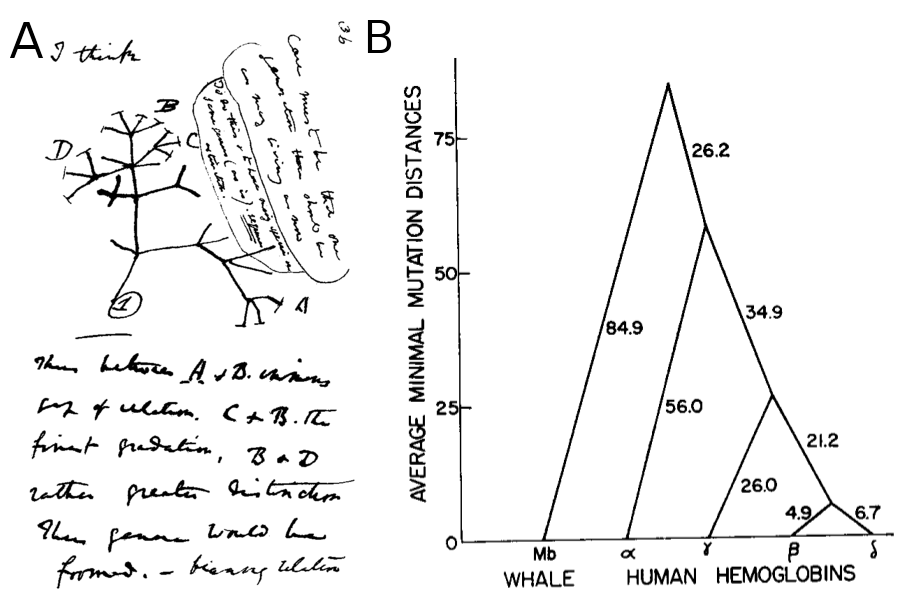
\includegraphics[scale=0.6]{first_trees} 
\caption{
{ \footnotesize 
{\bf Phylogenetic trees.} A. A page from Darwin's notebooks around July 1837 showing his first sketch of an evolutionary tree.
B. First phylogeny estimated from genetic data and published by \cite{Fitch1967}.
}% END: footnotesize
}
\label{fig:first_trees}
\end{figure}

%Underlying assumption of the phylogenetic tree is that the data used to infer them indeed encompasses some sort of evolutionary relatedness.
Phylogenetic thinking traces back to the first known figure of a phylogenetic tree, sketched by Charles Darwin in 1837 on the margin side of his notebook (see Figure \ref{fig:first_trees}), with the famous words \emph{`I think'} written above it.
In those days there was no notion of genetic data, therefore Darwin conceived his trees by comparing morphology, assuming that organisms with similar forms and shapes descended from more recent common ancestors. %\footnote{Furry with furry.}.
Modern phylogenetics use molecular data and a combination of statistical and computational methods to reconstruct phylogenetic trees.
%distance-based trees
Among the first tractable methods to reconstruct trees from molecular data were the hierarchical clustering methods based on genetic distance \citep{Fitch1967}, defined as the number of nucleotides that would need to be altered to make two sequences identical (see Figure \ref{fig:first_trees} B).
These methods were criticized for not making explicit use of the relationship between individual characters of the genetic data, but rather reducing it to distance-based measures.
%Moreover by using pairwise comparisons some of the information is inevitably lost.
Moreover, hierarchical clustering leads to a single point estimate of the evolutionary history and therefore does not consider alternative hypotheses for the data.

% parsimony
In order to evaluate different tree topologies the idea of parsimony was adopted in phylogenetics. 
Maximum parsimony approaches attempt to find the tree that requires the minimum number of evolutionary changes to explain the data. %, maing use of the whole data at once.
This concept stems from the work of William of Ockham (1320), who stated that among competing hypotheses one should select the simplest one and disregard the remaining more complex ones (Ockham's razor).
\cite{Edwards1963} formally introduced the idea into phylogenetics.
Later, \cite{Fitch1971} published an dynamic programming algorithm that efficiently searches all possible tree topologies, assigning scores to them and finding the one with minimal parsimony score.
Figure \ref{fig:parsimony} presents an example of parsimony, where among two trees explaining the evolution of sequences {\color{green}AAG}, {\color{green}AAA}, {\color{green}GGA}, {\color{green}AGA} only the most parsimonious one is selected.

%---PARSIMONY TREE---%
\begin{figure}[h!]
\centering
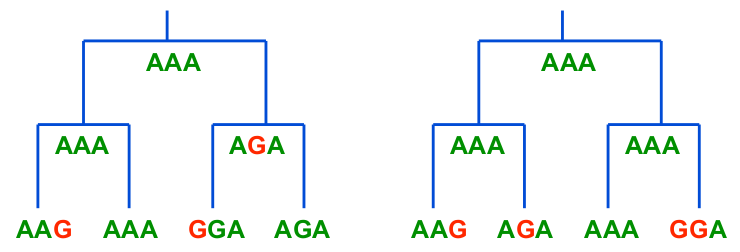
\includegraphics[scale=0.3]{parsimony} 
\caption{
{ \footnotesize 
{\bf Parsimony example.} The tree on the left is preferred as it requires the least amount of changes (3 substitutions as opposed to 4 for the tree on the right).
}% END: footnotesize
}
\label{fig:parsimony}
\end{figure}

%likelihood
As a statistical alternative to an optimality criterion, the likelihood had also been proposed for phylogenetic inference relatively early.
The idea of using maximum likelihood to estimate evolutionary trees was first proposed by \cite{Edwards1964}, although without a working implementation at the time of the publication.
Maximum likelihood is a probabilistic method of inference, that evaluates a hypothesis in terms of how probable it is in the light of the observed data.
In a phylogenetic setting, the likelihood function returns the probability that the proposed model and the proposed tree, understood as a topology and branch lengths, have generated the observed data.
\myedit{svthree}{
In general an evolutionary history and associated set of evolutionary parameters with higher probability of generating the observed data is naturally preferred over a history with a lower probability of generating it.
By using optimization techniques one can find the parameter values that maximize the probability of observing the data.
}
% The evolutionary history and associated set of evolutionary parameters with a higher probability is naturally preferred over a history with a lower probability.
% By using optimization techniques one can find the parameter values that maximize the probability of observing the data.
In his influential work, \cite{Felsenstein1981} proposed an efficient algorithm for calculating a likelihood of sequence evolution on a tree under an evolutionary model of substitution, the so called `tree pruning' algorithm.
Unfortunately finding the maximum likelihood tree requires a search through the space of all possible tree topologies; in section \ref{sub:mlburden} we discuss in detail the computational burden associated with these calculations.
The effort required to exhaustively search through a space of all possible rooted trees grows explosively with the number of taxa, as depicted in Table \ref{tab:maxLikeBurden}.

\begin{table}[h!]
\centering
% \footnotesize{
\begin{tabular}{cc}
% {@{}l*{2}{D{.}{.}{7}}@{}}
\hline 
Tips & Rooted trees $\frac{(2N-3)!}{2^{N-2}\cdot(N-2)!}$ \tabularnewline
\hline 
\rowcolor{gray1}
$3$ & $3$\tabularnewline
$6$ & $945$\tabularnewline
\rowcolor{gray1}
$9$ & $2'027'025$\tabularnewline
$15$ & $2\times10^{14}$\tabularnewline
\rowcolor{gray1}
$20$ & $8\times10^{21}$\tabularnewline
$55$ & $3.19\times10^{86}$\tabularnewline
\end{tabular}
% }
\caption{
{ \footnotesize 
{\bf{Number of rooted trees per number of taxa.}} For comparison, $4 \times 10^{80} $ is the number of atoms in the observable universe.
}% END: footnotesize
}
\label{tab:maxLikeBurden}
\end{table}

%bayesian
The advent of powerful and increasingly more attainable computing power has been instrumental to the adoption of statistical methods based on likelihood estimation and the closely related Bayesian methods.
Bayesian statistical thinking is not a new idea and stems back to the XVII century works of reverend Thomas Bayes, a statistician, philosopher and theologian. 

\clearpage

%---BAYES---%
\begin{remark}{Thomas Bayes}
\begin{figure}[H]
\centering
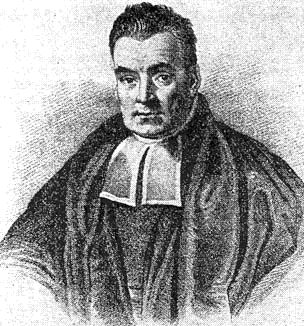
\includegraphics[scale=0.4]{Thomas_Bayes} 
\caption{
{ \footnotesize 
{\bf Only known portrait of reverend Thomas Bayes.} This portrait was published in the 1936 book on the history of actuarial science `History of Life Insurance'. It is only hypothesised to be an actual portrait of the scholar.
}% END: footnotesize
}
\label{fig:bayes}
\end{figure}
\end{remark}

Interestingly, Bayes has never published his famous work.
Bayesian statistics has always been appealing as a very flexible approach to inference, as it allows for inclusion of prior belief about any unknown parameters, which, combined with the likelihood of the data, forms an `updated' view of the model, the so-called posterior distribution.
This prior specification can reflect the degree of uncertainty we put into our belief and can be further enhanced by the use of the so called hyperpriors, prior distributions put on the parameters of first order priors.
Moreover, Bayesian inference allows for a natural interpretation of the results in terms of probability distributions. 
Unfortunately, calculating a posterior distribution requires the computation of integrals over the space of all possible parameter values, which are often multi-dimensional.
For a long time, this has limited its use for most but the simplest problems until \cite{Metropolis1953} proposed a Markov chain Monte Carlo (MCMC) algorithm for obtaining a sequence of random samples from a probability distribution for which direct sampling is difficult. 
Later, \cite{Hasting1970} extended and generalized the algorithm which came to be known as the Metropolis-Hastings method.

\begin{remark}{Monte Carlo}
Monte Carlo methods are computational algorithms that rely on computer-generated pseudo-random numbers to obtain numerical results. 
They were invented in the late 1940's by Stanis\l{}aw Ulam, while he was working on nuclear weapons for `project Manhattan'
at the Los Alamos laboratory.  
It was named after the Monte Carlo Casino in Monaco, where Ulam's uncle often gambled.
Monte Carlo was dubbed the most important algorithm of 21st century by the Society for Industrial and Applied Mathematics (SIAM).
\end{remark}

The Bayesian inference problem can be formulated as a sampling problem, as we discuss in Section \ref{sec:bayesian_inference}, reducing to a very simple and effective method, which contributed to the popularity of Bayesian statistics that we see today. 
The availability of programs for Bayesian phylogenetics like MrBayes \citep{Huelsenbeck2001} and BEAST \citep{Drummond2012} further contributed towards the widespread adoption and popularity of these methods in evolutionary biology.

\subsection{Time-calibrated trees and Measurably Evolving Populations\label{sub:clocks}}

%Molecular clock
The molecular clock hypothesis (\cite{Zuckerkandl1962}) posits that the rate of evolution of any specified protein remains roughly constant over time and over different lineages.
In particular, Zuckerkandl and Pauling observed that amino acids were replaced at a roughly constant rate in hemoglobins as judged from the fossil record.

% \begin{figure}[H]
% \centering
% 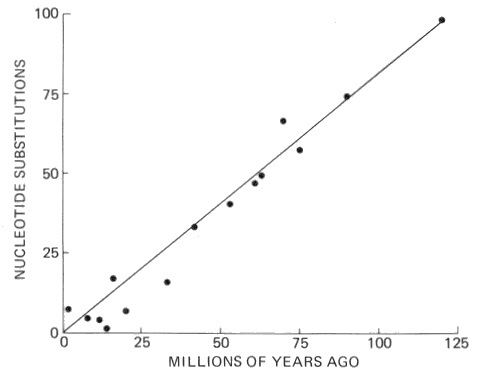
\includegraphics[scale=0.3]{molecular_clock} 
% \caption{
% { \footnotesize 
% {\bf Inferred pairwise nucleotide substitutions among 17 mammal species plotted against dates of divergence estimated from fossil records \citep{Wilson1976}.} Linear relationship suggests that pairwise molecular differences are proportional to the time of their separation, and not the morphological traits.
% }% END: footnotesize
% }
% \label{fig:molecular_clock}
% \end{figure}

This hypothesis is compelling because of its simplicity and because it provides a means to date bifurcation events on the tree of life.
A molecular clock assumption can only result in estimates of the proportion of time between two events. 
To estimate concrete dates for phylogenetic nodes, it needs to be calibrated using historical information such as  fossil records.
% MEPs
For rapidly evolving viruses however, it is possible to sample sequences that diverge over an observable timescale. 
As opposed to the ultrametric topology assumed for slowly evolving organisms (Figure~\ref{fig:ultrametric}), the dates of the samples themselves can be used to calibrate the molecular clock \citep{Rambaut2000}.

%---SAMPLING SCHEMES---%
\begin{figure}[h!]
\centering
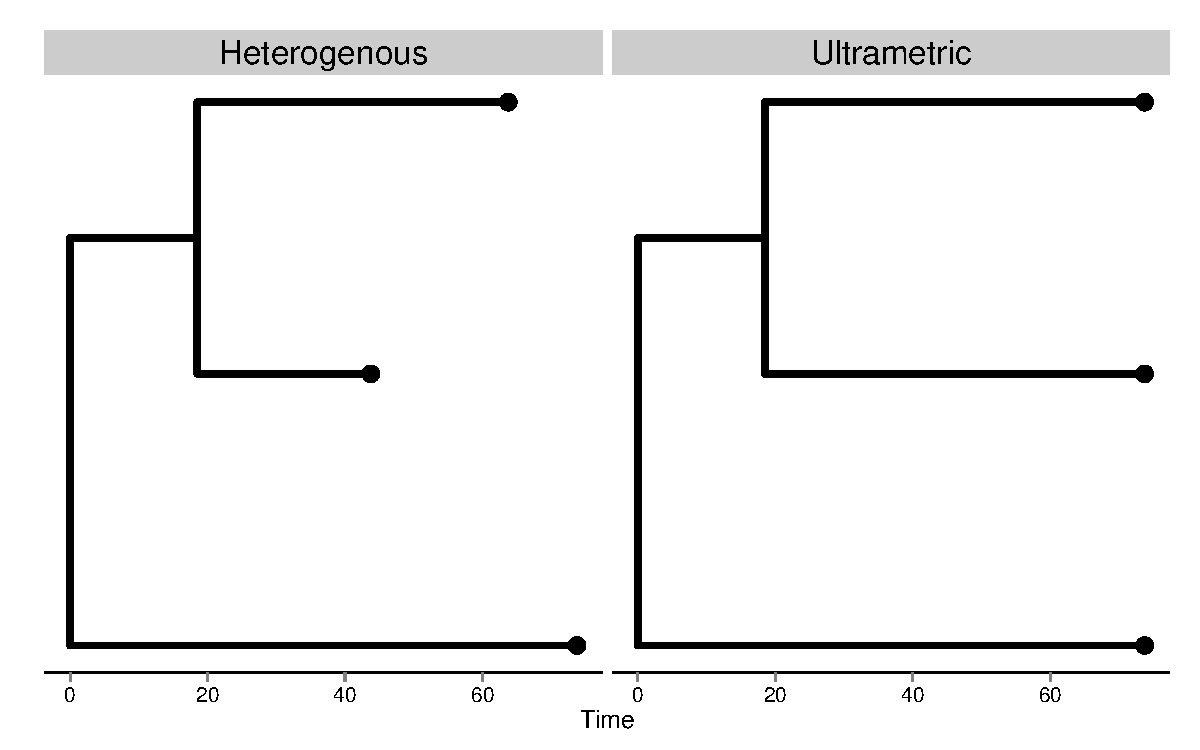
\includegraphics[scale=0.3]{ultrametric} 
\caption{
{ \footnotesize 
{\bf Different tree structures imposed by molecular clock assumptions for organisms evolving at different rates.} 
The tree on the right represents an evolutionary history of slowly evolving organisms, and has tips sampled in the last decades that are all aligned at $t=0$. 
Conversely the tree on the left represents an evolutionary history of rapidly evolving organisms with samples at different points in time in the last decades. 
By enforcing tip heights to be proportional to their sampling dates, temporal information is provided to calibrate the molecular clock for rapidly evolving organisms.
}% END: footnotesize
}
\label{fig:ultrametric}
\end{figure}

Time-stamped data sets have also been referred to as heterochronous data and %frequently arise from studies involving viruses which accumulate large amounts of genetic change in a relatively short amount of time.
populations for which such data can be obtained are called measurably evolving populations (MEPs, \cite{Drummond2003}).
This concept has been instrumental for providing estimates of evolutionary rates and for further developments in molecular clock modelling \citep{Drummond2006}.

% relaxed phylogenetics
It was realized relatively early that the molecular clock hypothesis is a simplifying assumption that may be violated by many biological systems.
Several studies demonstrated that the strict molecular clock hypothesis is often rejected for real-world data sets \citep{EyreWalker1997,Andreasen2001}, leading to widespread evidence for heterogeneous rates of evolution.
Unfortunately, the alternative `unconstrained' model, which estimates genetic distances for each phylogenetic branch, does not incorporate any relationship between sequence divergence and time and can therefore not be used for divergence time estimation.
%A naive approach to counter these problems is to allow for unconstrained changes in branch substitution rates on the whole tree.
%Unfortunately this does not facilitate the main advantage of the molecular clock hypothesis - the ability to date the speciation events.
This is due to the fact that genetic distances for branches in the unconstrained model are products of the substitution rate and the branch length in time units.
Without any assumption about the rates across branches, both quantities remain confounded (see also Subsection \ref{sub:rates}).

Because both the strict molecular clock model and the unconstrained model are unsatisfactory extremes, many developments aimed at `relaxed molecular clock' models, which allow for a changes in rate over time, but in a constrained manner and therefore still allowing to estimated divergence times.
\citet{Drummond2006}, for example, propose several uncorrelated relaxed clock models in which the substitution rate can vary among the branches of the tree by being drawn independently and identically from some underlying distribution.
Set in a Bayesian framework, this approach allows for a joint reconstruction of the topology and divergence times under less restrictive models.
Amongst others, a random local clock model approach has also been proposed \citet{Drummond2010} as a more discrete alternative, which allows identifying and quantifying a restricted number of rate changes throughout evolutionary history.
%The RLC model constructs proposal distributions which efficiently propose moves in both the tree space and in the clock rate space at the same time. %(see Subsection~\ref{sub:mcmc})
%Furthermore this approach favours parsimonious models with least parameters, utilizing the fact that for most datasets there exists only a small number of rate changes and that subclades on a tree will share the same rate.
This is achieved through a Bayesian Stochastic Search Variable Selection (BSSVS, \citet{Lemey2009}) procedure that lets the data decide which clock rate changes are needed to explain most rate variation.

\subsection{Processes giving rise to genealogies: demography and migration\label{sub:molecular_clock}}

Genealogies are trees that trace the ancestral and descendant relationships among individuals in a population.
The process describing how lineages on a genealogy merge to a common ancestor as we go back in time from the present is called the \textit{coalescent} \citep{Kingman1982}.
The simplest formulation of the coalescent process described by John Kingman was derived as an approximation of the \textit{Wright-Fisher} \citep{Fisher1930,Wright1931} population model (see Figure~\ref{fig:wright-fisher}).

%---COALESCENT---%
\begin{figure}[h!]
\centering
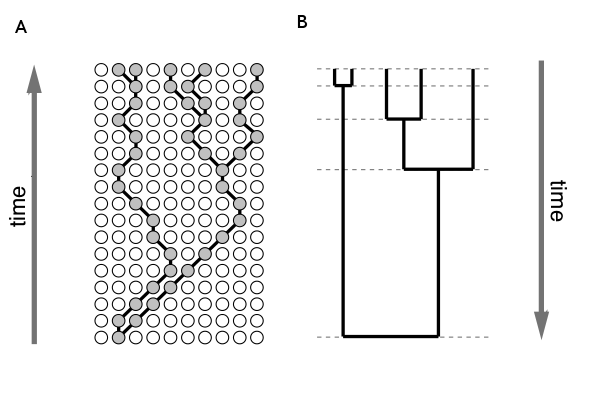
\includegraphics[scale=0.4]{wright-fisher} 
\caption{
{ \footnotesize 
{\bf The Wright-Fisher population model and Kingman's $n$-coalescent} A. A Wright-Fisher population of $N=10$ individuals. The lineages for all individuals sampled from the population coalesce to a common ancestor.
B.  In Kingman's $n$-coalescent, time is continuous and measured from tips towards the root.
}% END: footnotesize
}
\label{fig:wright-fisher}
\end{figure}

Under the Wright-Fisher model, the population size $N$ is assumed to be constant through time.
Time (generations) is discrete, i.e. every individual is replaced in every generation, with all individuals having equal chances of reproducing.
To understand how we can describe the coalescent process for a small sample of individuals from such populations as a function of their size, let us start with numbering time (generations), starting from present one as $t_{0},t_{1},t_{2},\ldots,t_{k}$.
The probability that two individuals sampled at the present generation $t_{0}$ share a common ancestor at a preceding generation $t_{1}$ is $\frac{1}{N}$.
The probability that two individuals sampled at $t_{0}$ share an ancestor at $t_{2}$ is the probability that they do not share an ancestor at $t_{1}$, which is $1-\frac{1}{N}$, times the probability of sharing an ancestor at $t_{2}$, which is $\frac{1}{N}$, as the population size remains constant every generation.

%\begin{remark}{Sir John Frank Charles Kingman}
%\begin{figure}[H]
%\centering
%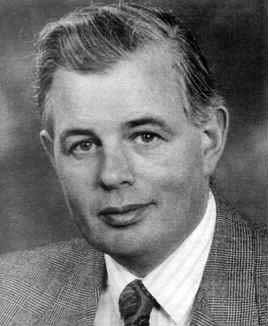
\includegraphics[scale=0.4]{kingman} 
%\caption{
%{ \footnotesize 
%% {\bf Sir John Frank Charles Kingman.} 
%This suave looking gentleman is a British mathematician, with his most notable work on the mathematics of the coalescent, a process fundamental to modern population genetics. 
%Interestingly Kingman never completed his PhD.
%}% END: footnotesize
%}
%\label{fig:kingman}
%\end{figure}
%\end{remark}

Generalizing this, we can write down the probability that a pair of randomly sampled individuals will have their most-recent common ancestor (MRCA) at time $t_{k}$:

\begin{equation}
P\left(t_{k}\right)=\left(\frac{1}{N}\right)\left(1-\frac{1}{N}\right)^{k-1}.
\label{eq:wright-fisher-two-individuals}
\end{equation}

\noindent
Now instead of sampling just two individuals we sample $n,\;2<n\leq N$ individuals, where $n\ll N$.
There are now $\frac{n\left(n-1\right)}{2}$ pairs in $t_{0}$ which can coalesce in $t_{1}$ and each pair has  $\frac{1}{N}$ probability of sharing the same ancestor, therefore:

\begin{equation}
P\left(t_{1}\right)=\frac{n\left(n-1\right)}{2N}.
\label{eq:wright-fisher-n-individuals}
\end{equation}

\noindent
Similarly as in the case of a pair of individuals we can generalize Equation~\ref{eq:wright-fisher-n-individuals} and write down the probability that the sampled pairs of individuals coalesce at $t_{k}$:

\begin{equation}
P\left(t_{k}\right)=\left(\frac{n\left(n-1\right)}{2N}\right)\left(1-\frac{n\left(n-1\right)}{2N}\right)^{k-1}.
\label{eq:wright-fisher-n-individuals-general}
\end{equation}

\noindent
Equation~\ref{eq:wright-fisher-n-individuals-general} characterizes a probability mass function (PMF) of a geometric distribution with parameter $p=\frac{n\left(n-1\right)}{2N}$ (see Equation~\ref{eq:geometric_dist}).

\begin{remark}{Geometric distribution}
The geometric distribution returns the probability that the $k$-th trial out of $k$ independent Bernoulli trials, each with success probability $p$, is a successful one:

\begin{equation}
P\left(X=k\right)=p\left(1-p\right)^{k-1},\;0<p\leq1,\; k\in\left\{ 1,2,3,\ldots\right\}.
\label{eq:geometric_dist}
\end{equation}

\noindent
Cumulative distribution function of the geometric distribution:
\begin{equation}
P(X\leq k)=1-\left(1-p\right)^{k-1}.
\label{eq:geometric_cdf}
\end{equation}
\end{remark}

For small values of $p$ the discrete geometric distribution can be approximated by its continuous equivalent, the exponential distribution. 
%An informal argument finds itself in Figure~\ref{fig:exp_approx}.
%
%\begin{figure}[H]
%\centering
%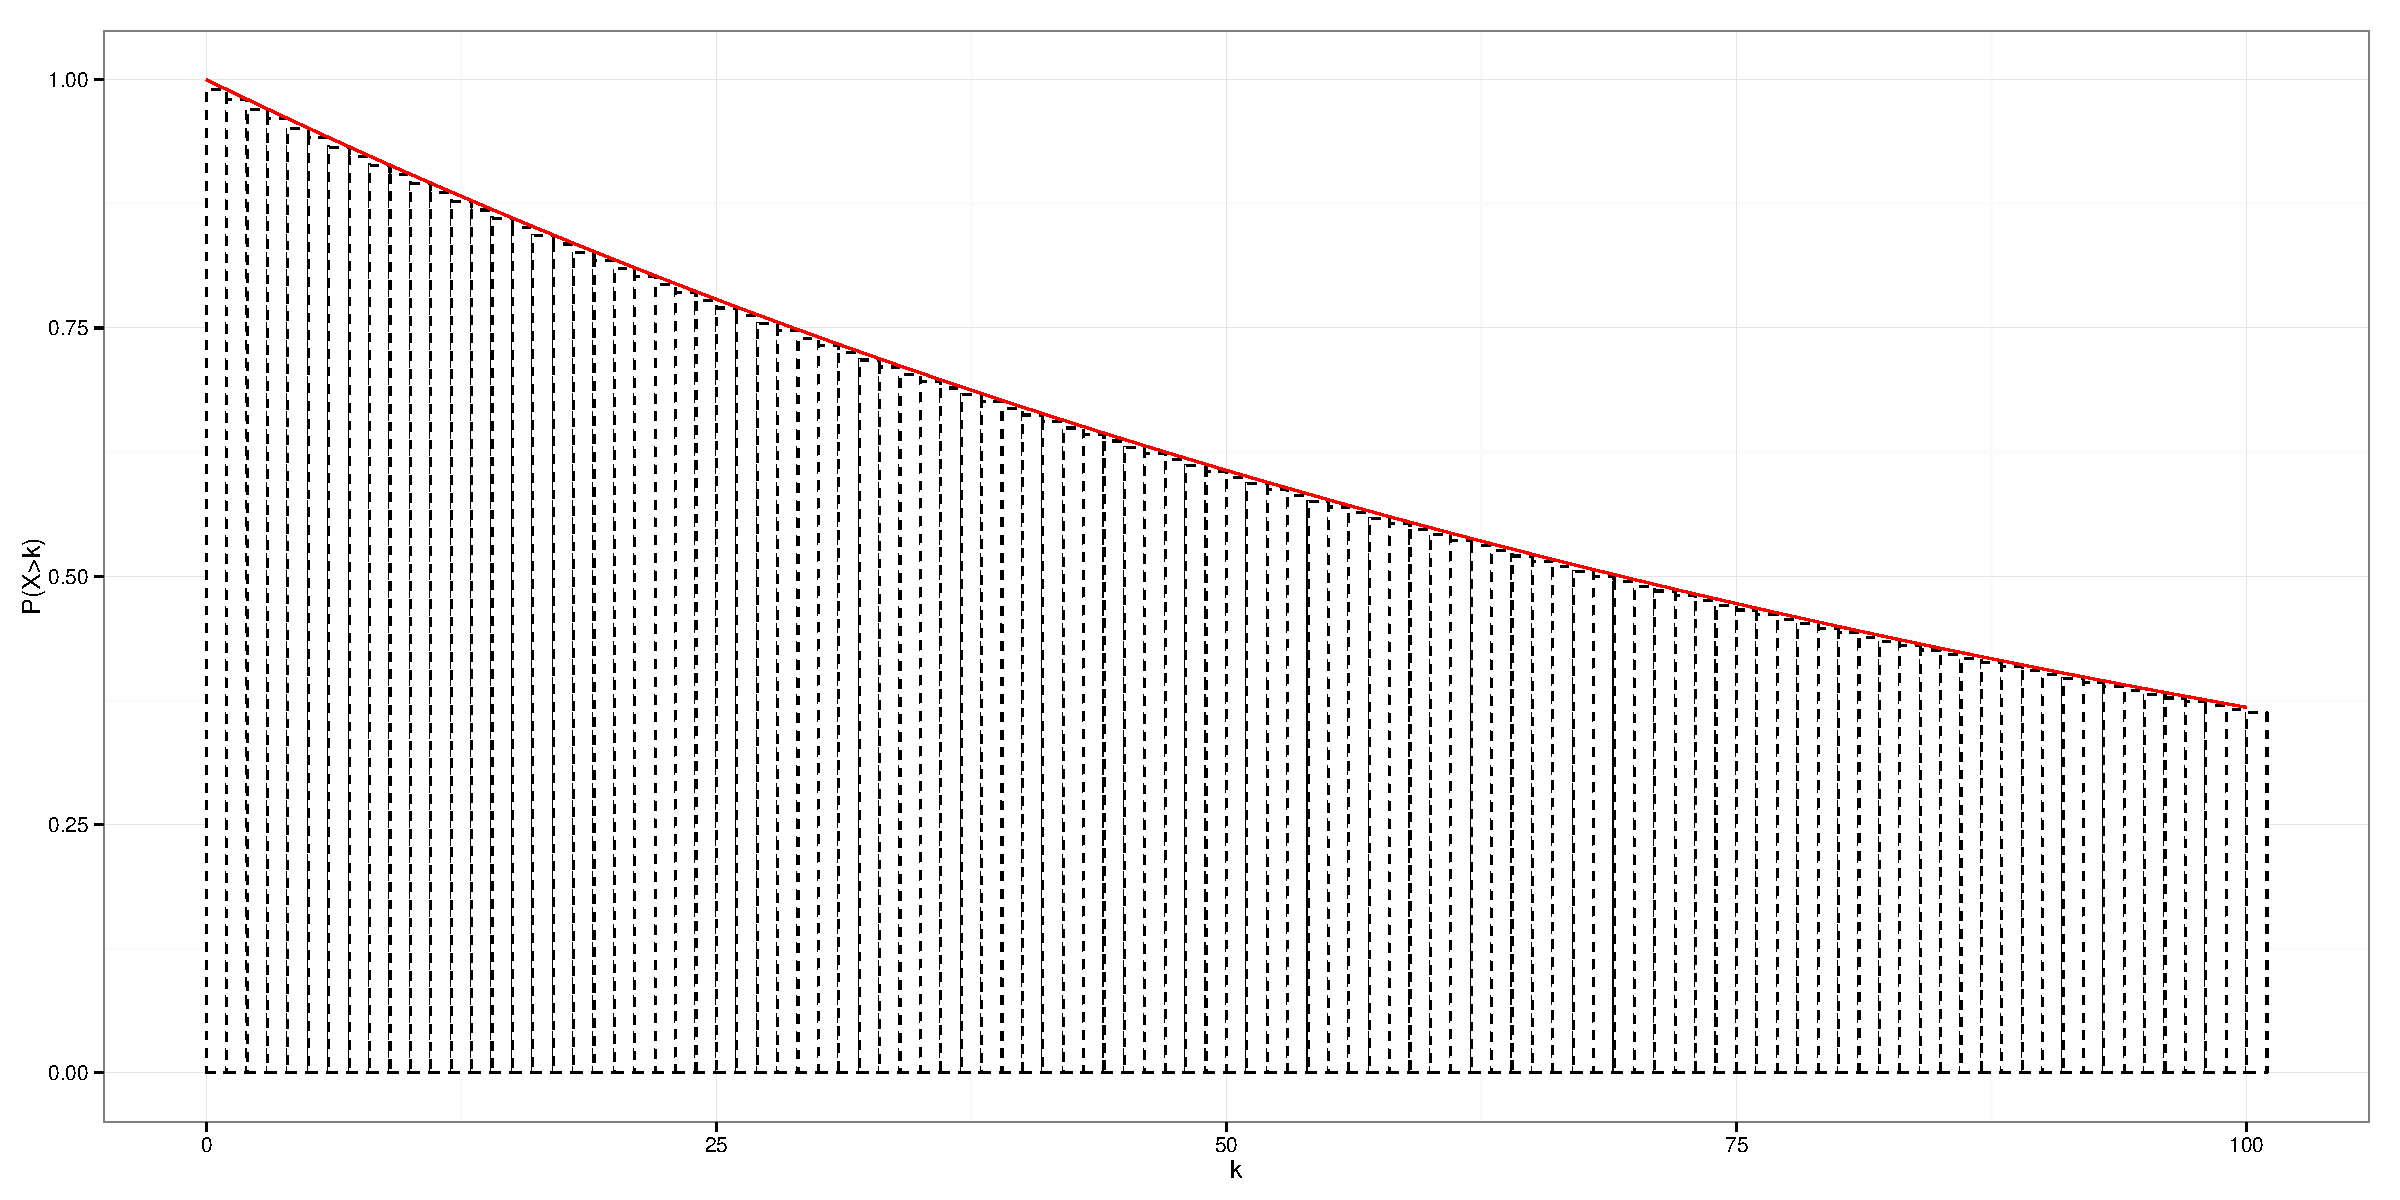
\includegraphics[scale=0.3]{exponential_approx} 
%\caption{
%{ \footnotesize 
%{\bf Approximating geometric distribution by exponential distribution.} 
%Black rectangles denote the discrete geometric distribution, red line is the continuous geometric distribution.
%}% END: footnotesize
%}
%\label{fig:exp_approx}
%\end{figure}
%
This approximation allows us to move into continuous time, and we can write Equation~\ref{eq:wright-fisher-n-individuals-general} as:

\begin{equation}
P\left(t_{k}\right)=\frac{n\left(n-1\right)}{2N}\textrm{exp}\left(-\frac{n\left(n-1\right)}{2N}k\right)
\label{eq:exponential_time}
\end{equation}

In the light of Equation~\ref{eq:exponential_time} we consider Kingman's coalescent as a continuous time version of the Wright-Fisher model with $n$ sampled individuals.
\cite{Rodrigo1999} developed an extension of Kingman's coalescent, the so-called \textit{serial coalescent} (s-coalescent), that allows to scale the genealogies in real time units.
Genealogies for a small sample of individuals can be estimated from their genetic data using phylogenetic reconstruction, and the resulting waiting time distributions in the trees can be used to estimate population sizes.
It is important to note, however, that these models make assumptions that are clearly violated in most populations and therefore lead to population size estimates that generally  deviate strongly from census population sizes. 
In order to still be able to use those models, a rescaling of the population model has been proposed so that it behaves, with regard to certain properties, as a simple Wright-Fisher model with constant population size.
This rescaling requires moving from census population size to the more abstract concept of `effective population size' or $N_{e}$.

As changes $N_{e}$ still reflect changes in the census population, the constant population size coalescent model has been extended to account for variable size populations, either in parametric \citep{Pybus2002} or non-parametric formulations \citep{Minin2008, Gill2013}. 
In a Bayesian framework focusing on time-measured trees, such process models find their use as priors on trees.
Coalescent models have also been extended to account for structured populations allowing to estimate migration rates, which naturally brings us to spatial dynamics \citep{Kuhner2006,migrate}.

% Introduce phylogeography
How geography impacts genealogies is one the main research questions of phylogeography, a discipline that frequently resorts to ancestral reconstruction to shed light on migration or dispersal dynamics. 
%Another process which shapes the phylodynamics of viral sequences is the process of their migration, which we understand as a dispersal in actual geographical coordinates.  
%Inference methods which make use of both molecular and geographical data have been dubbed as phylogeography as the processes which shape the genome are integrated with the processes of geographical spread.
In that sense, the inferred tree does not only provide a record of evolutionary ancestry, but also of the dispersal process that gave rise to the current geographic distribution of taxa.
%
%% snow
%Perhaps a first know study which used epidemiological methods which we today call phylodynamics, is the famous John Snow's work in 1854, tracing the source of a cholera epidemic in the Soho district of London.
%There was no notion of molecular data or even bacteria nor viruses, yet by using a dot map Snow was able to show that almost all the cases in were clustered in a close proximity of a water pump on the Broad Street (see Figure~\ref{fig:snow}).
%Snow was able to persuade local authorities to remove the handle, which contributed to the end of the outbreak.
%It was later found that a nearby cesspool was in fact leaking its content into the public well, therefore transmitting water contaminated with the cholera bacteria.
%
%\begin{figure}[H]
%\centering
%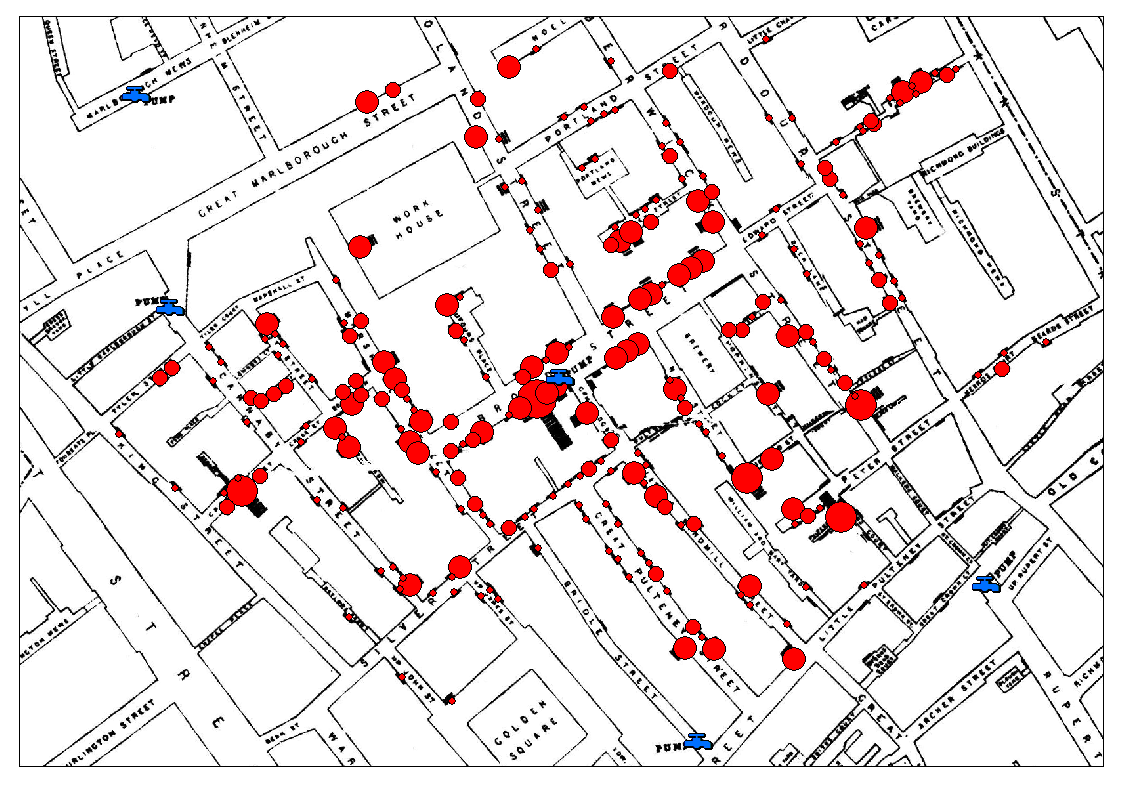
\includegraphics[scale=0.4]{snow_map} 
%\caption{
%{ \footnotesize 
%{\bf Map of the cholera cases in the London epidemic of 1854.} 
%Map shows the clustering of cases around water pump on the Broad Street (currently called Broadwick Street).
%}% END: footnotesize
%}
%\label{fig:snow}
%\end{figure}
%
% stochastic model based
In their opinion piece on current methods in phylogeography, \cite{Bloomquist2010} highlight fully probabilistic approaches that use Continuous-time Markov chain (CTMC) models to infer transitions between discrete locations as a function of continuous time as one of the phylogeographic inference methods.
Maximum likelihood and closely related Bayesian inference methods assume that both evolution and geographical dispersal are independent, stochastic processes which unfold on phylogenetic trees.
\cite{Lemey2009} and \cite{Lemey2010} developed a Bayesian framework that allows for a joint reconstruction of spatial diffusion and genetic ancestry, accommodating important sources of uncertainty in estimating spatial and temporal dynamics.
Because they are both modeled using CTMCs, the work presented here on CTMC model extensions finds applications to sequence evolutionary processes as well as these phylogeographic processes.

% population genetic / migration models
%The coalescent which we described at the beginning of this Subsection, and more generally population genetic approaches are another statistical inference method that can be naturally extended for phylogeography.
%These methods assume that trees are shaped by processes such as migration, selection or fluctuations in the population sizes in time.
%Trees proposed by the coalescent are then random draws from a larger, population-level processes, and one can use molecular and other data to get a better resolution of these underlying processes.

\subsection{Bayesian evolutionary inference in BEAST}

The Bayesian evolutionary analysis by sampling trees (BEAST) software \citep{Drummond2012}, to which our research group contributes, integrates many of the advances described in Subsections~\ref{sub:epidemiology}-\ref{sub:molecular_clock}.
BEAST is set in a Bayesian statistical framework, meaning that it combines the data likelihood (see Subsection~\ref{sub:likelihood}) with prior knowledge (see Section~\ref{sec:bayesian_inference}), and generates posterior samples using MCMC (see Subsection~\ref{sub:mcmc}).

% other packages
BEAST is not the only software package for Bayesian phylogenetic analysis and can be compared to a number of other packages.
MrBayes \citep{Huelsenbeck2001} is a command-line driven software mainly focusing on phylogenetic inference.
Migrate-n \citep{migrate} and LAMARC \citep{Kuhner2006} on the other hand concentrate on coalescent-driven population genetics.
At the core of BEAST lies a Metropolis-Hasting algorithm (\cite{Metropolis1953, Hasting1970}, see also Subsection~\ref{sub:mcmc}) for constructing Markov chains that converge on the posterior distribution as the equilibrium distribution.
This is precisely why BEAST is not meant for reconstructing a single tree or a point estimate for a parameter of interest, but rather generates samples that can be used to summarize distributions of mutation rates, divergence times, demographic parameters, trait evolution or others.

%beast
Compared to other similar programs, BEAST stands out in the number of models available for performing inference and the flexibility by which they can be combined.
Perhaps the most characteristic point is that BEAST uniquely focuses on sampling rooted, time-measured phylogenies.
This allows for a very natural interpretation of reconstructed trees, and is achieved thanks to the adoption of molecular clock models, from a simple strict clock model, with an equal rate across the whole time-span of the evolution, to relaxed molecular clock models that model rate variation in various ways \citep{Thorne1998,Yoder2000,Drummond2006,Drummond2010}.
BEAST offers a large number of complementary evolutionary models, which can be combined in a flexible way.
Various substitution models for performing analysis on nucleotide, codon or amino-acid data, accounting for among-site and among-lineage rate variation and partitioned in arbitrary ways, are complemented with demographic tree priors such as coalescent \citep{Drummond2005,Minin2008b} or birth-death priors \citep{Nowak2006} and trait evolutionary models.

% using beast
%The program takes as input structured XML files which describe the data to be analyzed, the models to be used, the number of samples to collect from the posterior and the output options.
%The output consists of a simple tab-separated files, with each row corresponding to one value sampled from the posterior distribution, for both the parameter values and actual trees.

%gpus
\myedit{DPfive}{
% The growing availability of large complex data-sets has led to the term `Big Data'. %being coined.
% Large sample sizes, such as full genome sequences or the ones generated with next-generation sequencing techniques are increasingly challenging phylogenetic inference.
Growing availability of large sample size, complex data-sets such as full genome sequences or the ones generated with next-generation sequencing techniques are increasingly challenging phylogenetic inference.
}%END: myedit
Fortunately strategies have been proposed to reduce the time that it takes to fit complex phylogenetic models to vast amounts of data.
These solutions are mainly focused on parallellization and on harnessing the capabilities of modern graphics processing units (GPUs), such as the NVIDIAs Tesla line of GPUs that target the high performance computing market.
BEAGLE (Broad-platform evolutionary analysis generalized likelihood evaluator, \cite{Ayres2012}), is a library that can be used in conjunction with BEAST and provides an API (Application Programming Interface) that massively parallel graphics processors and other multicore devices can exploit to substantially decrease the runtime of phylogenetic analysis \citep{Suchard2009}.
%BEAST readily integrates with BEAGLE and provides a GUI interface to configure the library.

% external software
BEAST is packaged with a number of additional utilities that can either assist in generating the input for BEAST, in analyzing the results or in some other specific tasks.
\textbf{BEAUti} (Bayesian Evolutionary Analysis Utility) is a  GUI (graphical user-interface) application for generating XML input files for BEAST. 
% It alleviates some of the most cumbersome tasks that would otherwise have to be done manually, thus saving time and simplifying 
It supports the specification of (standard) models, priors, operators, and MCMC chain settings, without having to resort to a manual editing of the XML syntax.
\textbf{LogCombiner} combines log files from multiple runs, that can then be imported into \textbf{Tracer}, a graphical tool for the analysis and visualization of the output of BEAST as well as other common MCMC packages.
It allows for a quick inspection of mixing, convergence, and summary statistics of the parameters of interest.
\textbf{TreeAnnotator} summarizes the tree log files and generally represents the evolutionary history using a maximum clade credibility (MCC) tree; each node or branch in this tree can be annotated with external information, such as posterior probabilities and maximum a posteriori ancestral traits.
The tree and its annotated information can subsequently be visualized using \textbf{FigTree} (\url{http://tree.bio.ed.ac.uk/software/figtree/}). % or if nodes of the trees are annotated with spatial information they can be displayes in geographical coordinates using \textbf{SPREAD}. %PL we need to introduce spread first, which is a chapter in this thesis :-), same for piBUSS
%Finally \textbf{$\pi$BUSS} is a software for sequence simulation, capable of generating XML files understood by BEAST for combined simulation-inference analysis as well as sequences in formats taht can be imported into any other phylogenetic software.
%
In conclusion, BEAST is a flexible package for statistical pylogenetics and hypothesis testing.
The software is continuously being improved and new models are being developed, but the development has recently been split into a continuing BEAST1 branch and a new BEAST2 branch\citep{Bouckaert2014}. 
Since the work presented in this thesis is implemented in BEAST1, all references to BEAST will implicitly refer to this development branch.
%In addition to a large array of available models, it is actively developed with new models and enhancements included with every new stable release.

\subsection{Objectives: model extension, simulation and visualisation\label{sub:objectives}}

% models
\paragraph{}
Phylogenetic analyses employing stochastic processes make strong restrictive assumptions regarding the underlying substitution process.
These assumptions are mainly enforced to reduce the number of free parameters of the models and to ease computational and mathematical tractability.
Unfortunately, many of these assumptions hamper the application of the methods to complex, real-world data sets.
Relaxing some of these assumptions and developing more biologically plausible models, able to grasp the complex nature of phylodynamic dispersal processes is an important aim of this thesis \citep{Bielejec2014a}.
%Another goal is to make the general applicability suitable for epidemiological problems as well as beyond them, with potential to turn the findings into useful predictions of the emergence of infectious diseases, e.g. by identifying the sources and sinks of the viral spread.
% geographical dispersal

% simulation
\paragraph{}
The development of novel phylogenetic inference methods brings about the need to compare estimator performance and to characterize strengths and weaknesses of different approaches (e.g. \cite{Arenas2012}, \cite{Hoban2011}).
Whereas the true underlying evolutionary relationships between biological sequences are generally unknown, Monte Carlo simulations allow to generate test scenarios while controlling the evolutionary history as well as the tempo and mode of evolution. 
Part of the research presented in this thesis is devoted to the development of flexible software for sequence simulation, that integrates both the tree-generative processes, as well as models responsible for shaping the molecular histories and geographical dispersal \citep{Bielejec2014a}.

% visualisation
\paragraph{}
Bayesian phylogenetic inference inevitably results in complex, multi-dimensional output.
Adding the geography to the phylogenetic process further adds to this complexity.
In particular, Bayesian phylogeography results in posterior distributions of trees, with each tree branch annotated with estimated node locations and other traits of interest.
%This represents a major challenge for visualization  the phylogenetic inference.
Clear and intuitive visualizations are an important aspect of every analysis \citep{Hadley2010}, but this is far from trivial for the estimates resulting from Bayesian analysis of sequences and traits.

Spatial phylogenetic projections have already been utilized in the field \citep{Kidd2006,Parks2009}, yet most of these applications remain limited to mapping phylogenetic tip taxa to their geographical coordinates, without providing robust statistical estimates of the geographic locations at the ancestral nodes nor the measures of uncertainty in the inference.
Fortunately, the advent of powerful and flexible Geographic Information Systems (GIS) has fostered an interesting possibility to visualize both the spatial and temporal information resulting from viral phylogenetic analysis.
Presenting readily interpretable visual summaries of the inferences that can be communicated to the researchers across different fields is one of the more important aspects of this thesis.

\section{Evolution as a stochastic process\label{sec:markov}}

In order to provide a formal basis for the work in the research chapters of this thesis, this chapter proceeds with a description of general stochastic models of character substitution processes in phylogenetics. 
Molecular phylogenetic modeling typically starts with an assumption that the observed sequence data has been generated by some stochastic process, which emits characters over time.
We can think of these stochastic processes as functions of time, which is regarded as a deterministic argument, whose values are random (non-deterministic) variables. 
It is thus a statistical model of a random development, or evolution, in time.
Phylogenetic inference often resorts to processes where time is considered to be continuous and the indexed set of outcomes, called the state space, is countable and finite (discrete).
With that in mind we can provide a formal definition:

\begin{definition} 
The stochastic process $X$ is a collection $\left\{ X(t):\; t\in T\right\} $, where each drawn value $X(t)$ is a random variable drawn from state space $\mathcal{E}$, with $K$ possible values, indexed by orderer time $T$.
\label{def:stochasticProc}
\end{definition} 

In the simplest case, for which the unit of evolution is a single nucleotide, we have $\mathcal{E}=\left\{ A,C,G,T\right\}$ and $K=4$.
%GB: perhaps point out that they're in fact not independent?
The particular sites of the sequence alignment are then considered to be stochastically independent realizations of the process $X$, leading to the observed data (see Figure~\ref{fig:alignment}). 


%PL: Since you list the mutations for the right branch, you may as well list the one on the left branch as well
% FB: not sure what you mean, should I add some annotation on that branch? I explicite left it empty, the right branch is longer so it has more substitutions on it than the left one
\begin{figure}[h!]
\centering
\begingroup
\everymath{\displaystyle}
{\Large
\begin{displaymath} % 
\xymatrix{
& \color{gray2}A \ar[dl] \ar[drdr]^{ \color{gray2}\begin{array}{c}
A\rightarrow G\\
G\rightarrow C
\end{array}} & & \\
T & & & \\
& & & C \\
}
%     \xymatrix@R+1pc{ 
% \color{gray2}A \ar[r] & \color{gray2}T \ar[r] & A \\
% \color{gray2}A \ar[r] & \color{gray2}T \ar[r] & G \\
% \color{gray2}A  \ar[rr]_{ \color{gray2}\begin{array}{c}
% A\rightarrow G\\
% G\rightarrow C
% \end{array}} &&  C
%     } % 
\end{displaymath}
}% END: Large
\endgroup
\caption{
{ \footnotesize 
{\bf Evolution at a single site.} Over time characters at the site change, leading to the observed data (black). 
%Some of the mutations may be unobserved. %PL: All mutations are unobserved!!!!
Each site evolves independently.
The longer the evolutionary time, the higher the probability that multiple substitutions occur on the same site.
}% END: footnotesize
}
\label{fig:alignment}
\end{figure}

As illustrated in Figure~\ref{fig:alignment}, multiple substitutions (multiple hits) may occur, which complicates the estimation of the underlying evolutionary distances from the observed data.
Specifically, the number of observed differences in the sampled genetic data will be an underestimate of the underlying genetic distance (in Figure~\ref{fig:alignment}, three substitutions underlie a single difference in the observed states).
In order to accurately describe these processes, one needs a model of evolution that can account for those multiple hits.

\subsection{The Poisson process\label{sub:poisson}}

The Poisson process is an example of a continuous-time stochastic process that is frequently used to describe counts of independent, rare events, occurring with some intensity (or rate) $r$, that remains constant over time. 
Examples of such a process are the requests for a single document on a web-server, or the goals scored in a football game \footnote{Unless it's Real - Barca, than the events are not so rare.}. %PL or Brazil - Germany...
%The state space in this case is obviously $\mathcal{E} = \left\{ 0,1,2, \dots \right\}$.
The Poisson process is equally suitable to model the number and waiting times of DNA mutation of sequence substitution events. 
We can formally define a Poisson process as following:

\begin{definition} 
A Poisson process with rate $r>0$ is a continuous-time counting process $\left\{ N(t):\; t\geq0\right\}$ such that:

\begin{itemize}
\item $N(0)=0$.
\item The increments are independent i.e. if $(t_{1},t_{2}]\cap(t_{3},t_{4}]=\emptyset$ then $N(t_2)-N(t_1)$ and $N(t_4)-N(t_3)$ are independent and stationary (i.e. the probability distribution of the number of occurrences counted in any time interval only depends on the length of that interval).
\item The number of events in any interval of length $t$ is $\text{Poisson}(r t)$.
\end{itemize}

\label{def:poisson}
\end{definition}

Figure~\ref{fig:poisson} shows a sample of different trajectories for such a process.

\begin{figure}[h!]
\centering
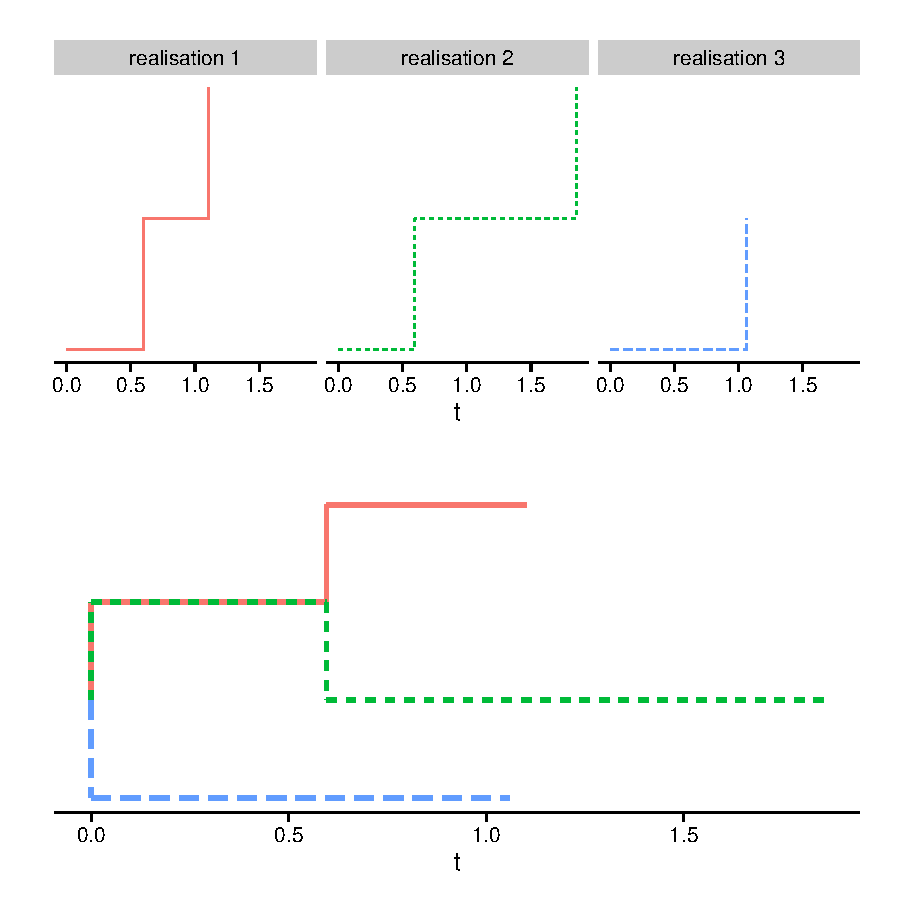
\includegraphics[scale=0.4]{poisson}
\caption{
{ \footnotesize 
{\bf Three independent realizations of the Poisson process with intensity $r=1$.}
Waiting times between mutations are \emph{iid} exponentially distributed random variables with mean $1/r$.
} % END: footnotesize
}
\label{fig:poisson}
\end{figure}

Let's assume that evolution at a single site is governed by a Poisson process $N$ with some intensity $r$.
Definition~\ref{def:poisson} implies that under this model the number of mutations $N(t+u)-N(u)$ in some time interval $(u,t+u]$ of length $t$ follows a Poisson distribution with expected number of events $r t$.
Thus we can write:

\newpage

\begin{align}
P\left\{ N(t+u)-N(u)=k\right\} & = P\left\{ N(t)=k\right\} \nonumber \\
= \frac{e^{-r t}(r t)^{k}}{k!},\; k=0,1,\ldots
\label{eq:poissonDist} 
\end{align}

In the Poisson process the time between any two mutations is exponentially distributed with parameter $r$, thus the average waiting time between the occurrence of events is $1/r$.
To show this important property we can consider $T_1,T_2,\ldots$ to be the inter-arrival times, where $T_k$ is the waiting time between the $(k-1)\text{'st}$ and $k\text{'th}$ mutation. 
Obviously, the number of mutations before some time $t>0$ is less than some integer $k>0$ if and only if the waiting time $T_k$ until the $k\text{'th}$ mutation is larger than $t$:

\begin{equation}
P\left(N(t)<k\right)=P\left(T_{k}>t\right).
\end{equation}

\noindent
For the first waiting time $T_1$ we have:

\begin{equation}
1-P\left(T_{1}>t\right)=1-P\left(N(t)<1\right)=1-P\left(N(t)=0\right).
\end{equation}

\noindent
From Equation~(\ref{eq:poissonDist}) we have that:

\begin{equation}
F_{T_{1}}(t)=1-P\left(T_{1}>t\right)=1-e^{-r t}.
\end{equation}

\noindent
$T_1$ therefore follows the exponential distribution with parameter $r$.
For the second waiting time $T_2$ and some arbitrary $u>0$ and $t>0$, the independent increments property implies that:

\begin{eqnarray}
F_{T_{2}}(t) &=& 1-P\left(T_{2}>t|T_{1}=u\right) \nonumber \\
& = & 1-P\left(\text{no mutations in }(u,t+u]|T_{1}=u\right) \nonumber \\ 
& = & 1-P\left(N(t)=0\right)=1-e^{-r t}.
\end{eqnarray}

\noindent
Therefore, $T_2$ is independent of $T_1$ and $\text{Exponential}(r)$ distributed. 
Similarly we can show that $T_3$ is independent of $T_1$ and $T_2$ and by repeating the same argument: $T_1,T_2,\ldots$ are independent and identically distributed (i.i.d.) $\text{exponential}(r)$ random variables.

% TODO: memoryless property does not depend at all, vide poiss)
% TODO: markovian (depends only a little)
% * difference? Memoryless is more

\subsection{Instantaneous rates of mutation\label{sub:rates}}

Within a phylogenetic framework the interest typically lies not only in modeling the number of events (mutations), but also the actual probabilities of changing states at the particular site in the alignment. 
We therefore need to generalize the process to a finite number of discrete states.
Let $\mathbf{R}$ denote a $K \times K$ matrix filled with probabilities of exchanging states between any pair $i,j\in \mathcal{E}$.
To express the probability of going from state $i$ to $j$ in some time interval $t$, we multiply the probability of the state change by the probability of having exactly $k$ events leading to the observed change, and integrate over all possible values of $k$.
This allows us to accommodate all possible paths that evolution might have taken, and to account for multiple hits that might have occurred at the site, as illustrated in Figure~\ref{fig:alignment}.
From Equation~(\ref{eq:poissonDist}) we know the probability of having $k$ mutations in time interval $t$, thus:

\begin{equation}
\left\{ P(t) \right\} _{ij}= \left\{ \underset{k=0}{\overset{\infty}{\sum}}\mathbf{R}^{k}\frac{(r t)^{k}}{k!}e^{-r t} \right\} _{ij} = \left\{ \underset{k=0}{\overset{\infty}{\sum}}\frac{(\mathbf{R}r t)^{k}}{k!}e^{-r t} \right\} _{ij},
\label{eq:matrixExp1}
\end{equation}

\noindent
where $\left\{  \cdot \right\} _{ij}$ denotes the $ij\text{-th}$ element of a matrix.
% the transition probability matrix $\mathbf{P}$ over time $t \geq 0$.
Let us denote the matrix $\mathbf{R}-\mathbf{I}$, where $\mathbf{I}$ is a $K \times K$ identity matrix, by $\mathbf{Q}$.
Using the power series definition of the transition probability matrix: $\exp(\mathbf{R})=\underset{k=0}{\overset{\infty}{\sum}}\mathbf{R}^{k}/k!$, we can write Equation~(\ref{eq:matrixExp1}) as:

\begin{equation}
\left\{ \left\{ P(t)\right\} _{ij} \right\} _{ij} = \left\{ e^{\mathbf{R}r t}e^{-r t} \right\} _{ij} = \left\{ e^{(\mathbf{R}-\mathbf{I})r t} \right\} _{ij}= \left\{ e^{\mathbf{Q}r t} \right\} _{ij}
\label{eq:matrixExp2}
\end{equation}

\noindent
A single entry $q_{ij} \ge 0$ for $i \neq j$ in matrix $\mathbf{Q}$ quantifies the probability of changing from state $i$ to $j$ in an infinitely small amount of time, therefore we will refer to $\mathbf{Q}$ as the \emph{instantaneous rate matrix}.

\subsection{Computing the matrix exponent \label{sub:exponentiation}}

In order to arrive at the finite-time transition probability matrix $\mathbf{P}(t)$ for some time $t\geq0$, one needs to compute the matrix exponential in Equation~\ref{eq:matrixExp2}.
\cite{Moler1978} provide an excellent review of numerical methods to compute the matrix exponent. 
Here, we highlight the method utilized by most phylogenetic software, including BEAGLE \citep{Ayres2012} and BEAST \citep{Drummond2012}, that uses the singular value decomposition (SVD) of the rate matrix $\mathbf{Q}$.   

Let us assume $\mathbf{Q}$ has $K$ linearly independent eigenvectors $\mathbf{v}_{i} \; (i=1,\ldots,K)$ with corresponding eigenvalues $\lambda_{i}\;(i=1,\ldots,K)$:

\begin{equation}
\mathbf{Q}\times\mathbf{V}=\lambda\times\mathbf{V}
\label{eq:eigenvaluesEigenvectors}
\end{equation}

\noindent
This condition is sufficient for $\mathbf{Q}$ to be diagonizable, thus its Jordan form is:

\begin{align}
\mathbf{V}\times\mathbf{Q}\times\mathbf{V}^{-1}=\left[\begin{array}{cccc}
\lambda_{1} & 0 & \cdots & 0\\
0 & \lambda_{2} & \ddots & \vdots\\
\vdots & \ddots & \ddots & 0\\
0 & \cdots & 0 & \lambda_{K}
\end{array}\right] %\nonumber \\
= \text{diag}(\lambda_{1},\ldots,\lambda_{K})=\mathbf{D} ,
\label{eq:diagonalization}
\end{align}

\noindent where $\mathbf{V}$ is a matrix composed of eigenvectors of $\mathbf{Q}$. 
Multiplying both sides of Equation~(\ref{eq:diagonalization}) with the edge length $t$ and scaling by the appropriate rate scalar $r$, we can write $\mathbf{Q}$ in the following form:

\begin{equation}
rt\mathbf{Q}=\mathbf{V}\times\text{diag}(rt\lambda_{1},\ldots,rt\lambda_{K})\times\mathbf{V}^{-1} .
\end{equation}

\noindent Finally, using the power series definition of the transition probability matrix, we obtain: 

\begin{align}
\mathbf{P}(t) & =  \exp\left(rt\mathbf{Q}\right) \nonumber \\
& =   \underset{k=0}{\overset{\infty}{\sum}}\left(rt\mathbf{Q}\right)^{k}/k! \underset{k=0}{\overset{\infty}{\sum}}\left(\mathbf{V}\times\mathbf{D}\times\mathbf{V}^{-1}\right)^{k}/k! \nonumber \\
& =  \mathbf{V}\times\left(\underset{k=0}{\overset{\infty}{\sum}}\mathbf{D}^{k}/k!\right)\times\mathbf{V}^{-1} \nonumber \\
& =  \mathbf{V}\times\text{diag}(e^{rt\lambda_{1}},\ldots,e^{rt\lambda_{K}})\times\mathbf{V}^{-1} ,
\label{eq:eigen_decomposition}
\end{align}

\noindent 
where the last transition is due to the fact that the exponential of the diagonal matrix is obtained by exponentiating every entry on the main diagonal.
We should note here that the repeated evaluations of $\exp\left(rt\mathbf{Q}\right)$ for different times $t$ are all based on the same SVD of the matrix $\mathbf{Q}$. 
One needs only to scale and exponentiate the eigenvalues to calculate the diagonal matrix $D$ and perform two matrix multiplications, thus reducing all calculations to a simple and effective algorithm. 

\subsection{Markov chain models of sequence substitution\label{sub:subst_models}}

After obtaining finite-time transition probabilities given by Equation~\ref{eq:eigen_decomposition} for some time $t\geq0$ one can start drawing realizations, which follow probabilities defined by $\mathbf{P}$.
These realizations constitute a continuous-time stochastic process $\left\{ X(t):\; t\geq0\right\}$, which inherits the Markov property from the Poisson process modelling the time between any two mutations, as defined in Subsection~\ref{sub:poisson}.

We say that a stochastic process has the Markov property if the conditional probability distribution of future states of the process depends only upon the present state, not on the sequence of events that preceded it, i.e. for every $n\geq 0$, given the time points $0\leq t_{0}\leq t_{1}<\ldots<t_{n}\leq t_{n+1}$ and discrete states $i_{0},i_{1}, \ldots, i_{n},i_{n+1}$, it holds that: 

\begin{align}
& P\left\{ X(t_{n+1}) = i_{n+1}\mid X(t_{n})=i_{n},\ldots, X(t_{0})=i_{0}\right\}   \nonumber \\
&= P\left\{ X(t_{n+1}) = i_{n+1}\mid X(t_{n})=i_{n}\right\} .
\label{eq:markov}
\end{align}

The elements of $\mathbf{P}$ quantify the finite-time transition probabilities between the $K$ discrete state-space elements.
This describes a Continuous-time Markov chain (CTMC), which  we will use to model the substitution process at a single site of an alignment.
Every CTMC is completely characterized by its rate matrix $\mathbf{Q}$ and the stochastic matrix $\mathbf{P}(t),\ t\geq0$ is obtained via matrix exponentiation as described in the previous subsection (Subsection~\ref{sub:exponentiation}).

%---SUBSTITUTION MODEL---%
\begin{figure}[h!]
\centering
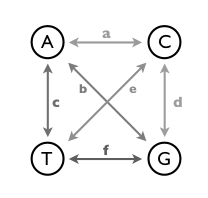
\includegraphics[scale=0.5]{substitution} 
\caption{
{ \footnotesize 
{\bf  Graphical representation of a nucleotide substitution model.} 
Markov substitution model with 6 parameters describing the symmetric transition rates.
} % END: footnotesize
}
\label{fig:substitution}
\end{figure}

Figure~\ref{fig:substitution} depicts an example of such a CTMC substitution model, governing the substitution rates between four discrete nucleotides, where all the pairs communicate (all states have a non-zero transitional probability, i.e. all states are non-absorbing).
Let us denote a transition probability between two states $i$ and $j$ over time $u$ to $t+u$ by:

\begin{equation}
p_{ij}\left(u,t+u\right)=P\left\{ X(t+u)=j\mid X(u)=i\right\} .
\end{equation}

In the phylogenetic setting, researchers often constrain the CTMC processes, mostly for computational and mathematical convenience.
A frequently applied restriction is to assume time-homogeneity of the substitution process, which states that the evolution does not change in pattern over time, and therefore transition probabilities depend only on the time difference $t$ between $u$ and $t + u$:

\begin{equation}
p_{ij}\left(t\right) = p_{ij}\left(0,t\right) = p_{ij}\left(u,t+u\right).
\label{eq:time_homogeneity}
\end{equation}

Unfortunately, this assumption does not hold for many real-world data-sets and precludes the identification of biologically interesting patterns in the evolutionary process. %, as the temporal dynamics clearly do shift in time, often in a seasonal, observable manner \citep{Bahl2011}.
%PL: deleted the above subsentence as it is too specific to phylogeography
One of the goals of the research presented in this thesis is to efficiently confront situations in which this assumption does not hold.
% can grasp such situations.

Substitution models are further constructed to be ergodic, meaning that there exist positive values $\pi_{1},\pi_{2},\ldots,\pi_{K}$ such that:

\begin{equation}
\forall i,j\in \mathcal{E}  \quad\underset{t\rightarrow\infty}{lim}p_{ij}(t)=\pi_{j}.
\label{eq:ergodicity}
\end{equation}

% $\mathbf{\Pi}$

As $t$ goes to infinity the probability that the site is in some state $j$ is non-zero and does not depend on the starting state $i$.
This implies that the chain will always display the same long-term behavior, which is why $\mathbf{\Pi}=\{\pi_{i},\ i\in\mathcal{E}\}$ is called a \emph{stationary distribution} (also referred to as the \emph{equilibrium distribution} or \emph{equilibrium frequencies}).
We can look at the elements of $\mathbf{\Pi}$ as the proportion of time spent in state $j\in\mathcal{E}$ after the Markov chain has run for infinitely long time, that does not depend upon the initial state $i$ of the process.
In other words, if we sample the initial state from the stationary distribution and then let the process run for some sufficiently long time $t$, then the distribution of the final state will equal the stationary distribution. 
\myedit{svsixone}{
From the biological perspective stationarity means that the probability distribution of a certain state (e.g. nucleotide character) is constant over the whole course of evolution; the probability to draw a certain state is the same whenever the sampling is done.
A process can be stationary and not be homogeneous, for example by varying substitution rates on the tree branches (see \cite{Yang2002} and the discussion in Subsection~\ref{sub:dpp}).
However the converse is not true, and non-stationarity induces non-homogeneity, as the stochastic process of evolution depends on the stationary distribution.
}

Another commonly applied constraint is that of \emph{time-reversibility}, meaning that the model does not care which character is the ancestor and which is the descendant so long as all other parameters are held constant.
For all $i,j\in \mathcal{E}$ and $t\geq 0$ we have:

\begin{equation}
\pi_{i}p_{ij}(t)=\pi_{j}p_{ji}(t).
\label{eq:time_reversibility1}
\end{equation}

\noindent
Condition~\ref{eq:time_reversibility1} is also referred to as the \emph{detailed balance} equation, and posits that the probability of sampling $i$ from the stationary distribution and then going to $j$ over some finite-time $t$ is the same as sampling $j$ and going to $i$. 
By the definition of $\mathbf{\Pi}$ and $\mathbf{P}$ from (\ref{eq:time_reversibility1}) the equality holds for infinitesimal rates:

\begin{equation}
\pi_{i}q_{ij}=\pi_{j}q_{ji}\mathbf{Q}.
\label{eq:time_reversibility2}
\end{equation}

Definition (\ref{eq:time_reversibility1}) and (\ref{eq:time_reversibility2}) are equivalent.

This condition is assumed for strictly computational reasons, i.e. time-reversibility makes it easier to diagonalize $\mathbf{Q}$, which - as we have described in Subsection~\ref{sub:exponentiation} - is a strategy frequently employed in phylogenetic software to compute the exponentials of rate matrices.
Time reversibility also simplifies the computation of the likelihood on a tree, since it makes the computation independent of the position of the root, which we will discuss in Subsection~\ref{sub:likelihood}.

\myedit{svsixtwo}{
Realistic substitution processes are however unlikely to be time-reversible, especially since abandoning stationarity and homogeneity assumptions implies abandoning reversibility of the evolutionary process.
Recently however procedures have also been developed to compute phylogenetic likelihoods under non-reversible models \citep{Boussau2006}, and such non-reversible models have also been explored for large state-space discrete phylogeographic applications \citep{Edwards2011}.
}

\subsection{A simple example: the Jukes and Cantor substitution model\label{sub:jc69}}

In this subsection we will discuss the simplest model of nucleotide substitution, i.e. the JC69 model \citep{Jukes1969}.
The JC69 model assumes that the instantaneous rates of change between every two nucleotides are the same.
It is also required that the rate matrix $Q$ characterizing the model is a stochastic matrix (each row sums to 0).
The infinitesimal rate matrix of the JC69 model is thus given by:

\begin{equation}
\mathbf{Q}=\left[\begin{array}{cccc}
-3r & r & r & r\\
r & -3r & r & r\\
r & r & -3r & r\\
r & r & r & -3r.
\end{array}\right]
\label{eq:jc69}
\end{equation}

\noindent
The finite-time transition probability matrix $\mathbf{P}(t)$ for time $t>0$ is calculated using matrix exponentiation  (see Subsection~\ref{sub:exponentiation}):

\begin{align}
% \mathbf{P}\left(t\right) &=& \left[\begin{array}{cccc}
% p_{0}(t) & p_{1}(t) & p_{1}(t) & p_{1}(t)\\
% p_{1}(t) & p_{0}(t) & p_{1}(t) & p_{1}(t)\\
% p_{1}(t) & p_{1}(t) & p_{0}(t) & p_{1}(t)\\
% p_{1}(t) & p_{1}(t) & p_{1}(t) & p_{0}(t)
% \end{array}\right]
%  ,  \nonumber \\
% &\text{where}& \ensuremath{\begin{cases}
% p_{0}(t)=\frac{1}{4}+\frac{3}{4}e^{-4rt}\\
% p_{1}(t)=\frac{1}{4}-\frac{1}{4}e^{-4rt}
% \end{cases}}.
p_{ij}\left(t\right)=\begin{cases}
\frac{1}{4}+\frac{3}{4}e^{-4rt} & \text{if }i=j\\
\frac{1}{4}-\frac{1}{4}e^{-4rt} & \text{otherwise}
\end{cases}
\label{eq:jc69Finite}
\end{align}

\noindent
A few things are worth mentioning about Equation~(\ref{eq:jc69Finite}).
If we let $t\rightarrow \infty$ we can see that $\forall i,j\; p_{ij}(t)=1/4$, which means that the equilibrium distribution for the JC69 model is: 

\begin{equation}
\mathbf{\Pi}=\left\{ \pi_{T}=1/4,\pi_{C}=1/4,\pi_{A}=1/4,\pi_{G}=1/4\right\}
\label{eq:jc69Steady}
\end{equation}

\noindent
Second, the rate and time in Equation~(\ref{eq:jc69Finite}) occur as a product, which means that rate and time are confounded.
If we were to simulate two sequences, using the algorithm listed in (\ref{alg:simulation}) and start the random number generators from the same seed, they will look the same for every $r$ and $t$ as long as their product $rt$ is the same.
This is true for most of the substitution models and implies that typical phylogenetic estimation focuses on inferring the product parameter $\theta=rt$, or genetic distance.
In Subsection~\ref{sub:clocks} we discuss how, under certain conditions, the time and substitution rate can be separated.

\subsection{Markov models of codon evolution\label{sub:codon}}


\myedit{svonea}{
First two computationally tractable codon substitution models were independently proposed by \cite{Muse1994} and \cite{Goldman1994} in the same issue of Molecular Biology and Evolution (MBE).
In these models, a non-stop codon triplet $n_{1}n_{2}n_{3}$ is considered to be the smallest unit of evolution.
According to the universal genetic code, there are $4^3$ possible triplets minus three stop codons, resulting in a state space size of $61$ codons.
The models inherit the standard assumption of independence, i.e. the substitutions at these three codon positions occur independently, and only a single change per triplet can occur at a given time. 
%%GB: explain in more detail, i.e. more than 1 change is possible in subsequent infinitesimal time intervals
Proteins are coded by a set of 20 amino acids, with each amino acid being coded by a codon triplet. 
Because there are 61 non-stop codons to encode for 20 amino acids, some amino acids will inevitably be coded by more than one codon.
A substitution that does not change the encoding amino-acid is called a \emph{synonymous} substitution, while a \emph{non-synonymous} substitution refers to a substitution that does result in an amino acid substitution.
Quantifying the rate at which these substitutions occur allows us to asses the nature of selective pressure, which is the main driving force behind molecular evolution.
}

That is why codon substitution models are generally parameterized in terms of the rate of non-synonymous (denoted by convention $\beta$) and synonymous ($\alpha$ by convention) substitutions or the ratio of these rates.
The rate ratio $\omega=\beta / \alpha$ is a standard measure of the selective pressure \citep{ThePhylogeneticHandbook}, which is sometimes also denoted $\omega = dN/dS$.
A higher rate of synonymous substitutions over non-synonymous can be interpreted as \emph{purifying (negative)} selection, and corresponds to a ratio $\omega <1$.
Non-synonymous substitutions accumulating at a faster rate than the synonymous substitutions is considered to be evidence for \emph{positive selection}, improving the fitness of the particular organism. Finally, $\omega\approx 1$ represents neutral evolution.

In addition to the ability to quantify selection, there are also other advantages in using codon models over nucleotide-based substitution models.
Not all DNA positions evolve at the same rate, with third codon positions generally evolving at higher rates than first or second codon positions because they are predominantly synonymous.
Although this problem can be mitigated to some extent by using codon-positioned nucleotide substitution models, the fast evolving positions and the state space limited to $4$ character alphabet still can lead to biased estimates over long evolutionary distances, as portrayed in the previous Chapter~\ref{chap:pibuss}.

For the remainder of this chapter we will focus on the GY94 model proposed by \cite{Goldman1994}, which is then utilized in the analysis performed in Chapter~\ref{chap:epoch} and in Chapter~\ref{chap:pibuss}.  
The Muse \& Gaut (MG94) model is discussed in Subsection~\ref{sub:dpp} of Chapter~\ref{chap:discussion}.

The GY94 model is characterized by a substitution rate matrix with following entries:

\begin{equation}
\left\{ \mathbf{Q}\right\} _{ij}^{GY94}=
\begin{cases}
\pi_{j} & \substack{ \text{ \ensuremath{i\rightarrow j} is a synonymous transversion from } \\ \text{codon \ensuremath{i} to \ensuremath{j} } } \\  
\kappa\cdot\pi_{j} & \substack{ \text{ synonymous transition } } \\
\omega\cdot\pi_{j} & \substack{ \text{ non-synonymous transversion } } \\
\omega\cdot\kappa\cdot\pi_{j} & \substack{ \text{ non-synonymous transition } } \\
0 & \substack{ \text{ otherwise} }
\end{cases},
\label{eq:gy94}
\end{equation}

\noindent
where the parameter $\kappa$ denotes the transition/transversion ratio, parameter $\omega$ denotes the non-synonymous/synonymous
rate ratio and $\pi_j$ denotes the equilibrium frequency of codon triplet $j$.
The parameters $\kappa$ and $\pi_j$ can be thought of as controlling the CTMC process at the DNA level, while the $\omega$ parameter characterizes the selection on non-synonymous substitutions.
For the GY94 model the synonymous evolutionary rate is fixed to be 1, i.e. $\omega=\alpha$.

\subsection{Phylogenetic trees}

%PL: According to the extension I recommend for the general intro, a tree should already be introduced properly there, and this should from the biological perspective but can also include this more formal description..

A phylogenetic tree, or phylogeny for short, depicts the genealogical relationship between character sequences.
Mathematically, a phylogeny $\mathbf{F}$ represents a directed, acyclic graph with sets of \emph{nodes} connected by \emph{branches} (e.g., Figure~\ref{fig:treeconcept}).
Data is observed only at the external nodes (\emph{tips}), while internal nodes represent extinct ancestors for which data is usually missing.
The ancestor of all observed samples is called the \emph{root} of the tree and its height is referred to as the time to the most recent common ancestor (TMRCA).

%---TREE CONCEPT---%
\begin{figure}[h!]
\centering
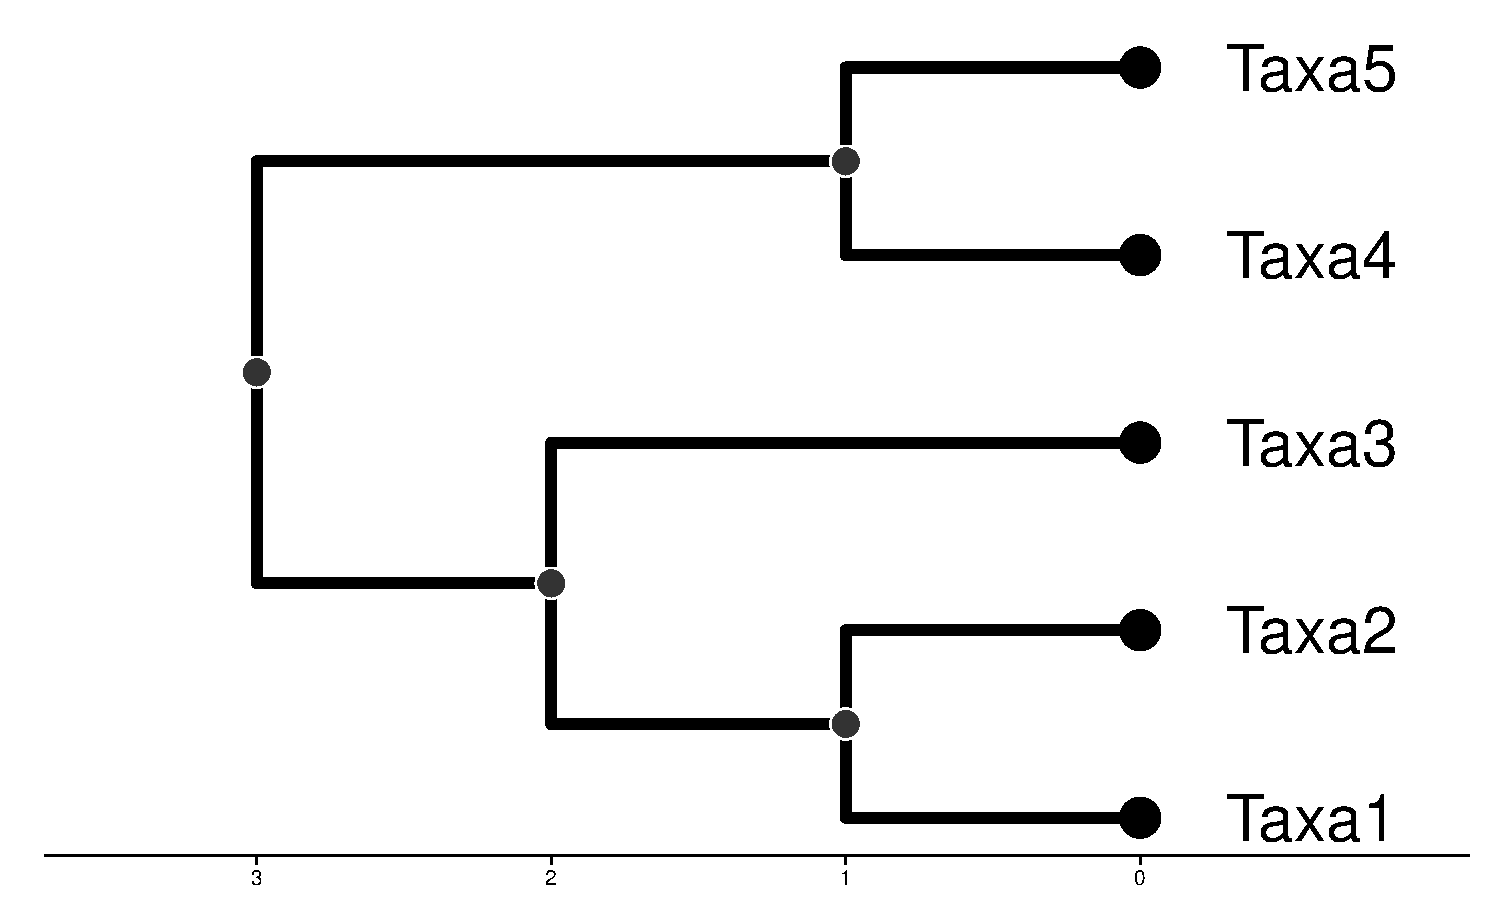
\includegraphics[scale=0.35]{treeconcept} 
\caption{
{ \footnotesize 
{\bf A phylogenetic tree showing evolutionary relationship.} Character sequences are observed at the tips of the tree (black dots); sequence characters at the internal nodes are treated as missing data (outlined dots). 
Branch lengths can be estimated in units of genetic distance, or as in this case, real time.
} % END: footnotesize
}
\label{fig:treeconcept}
\end{figure}

Within our framework we focus on trees which are rooted and time-measured, i.e. their branch lengths are scaled in actual time units.
A rooted binary tree with $n$ leaves has $2n-2$ branches and $n-1$ internal nodes.
The branching pattern of the tree is called the \emph{topology}. 

\subsection{Dated phylogenetic trees\label{sub:dated_trees}}

\myedit{svoneb}{
Time-stamped or `heterchronous' sequence data, which frequently arises from studies involving MEP populations for which sequences are sampled at different points in time and the evolutionary rates are high enough for significant changes to occur between the sampling times, can be used to calibrate the molecular clock and convert branch lengths into actual time units.
}
For simplicity let us assume a single site, where character sequence data was sampled on dates ranging from $1983$ to $2000$, as seen in Figure~\ref{fig:timing_sequences}.
We also assume that the rooted tree topology is known and we want to estimate the unknown times $T_{0},T_{6},T_{7},T_{8}$.

\begin{figure}[h!]
\centering
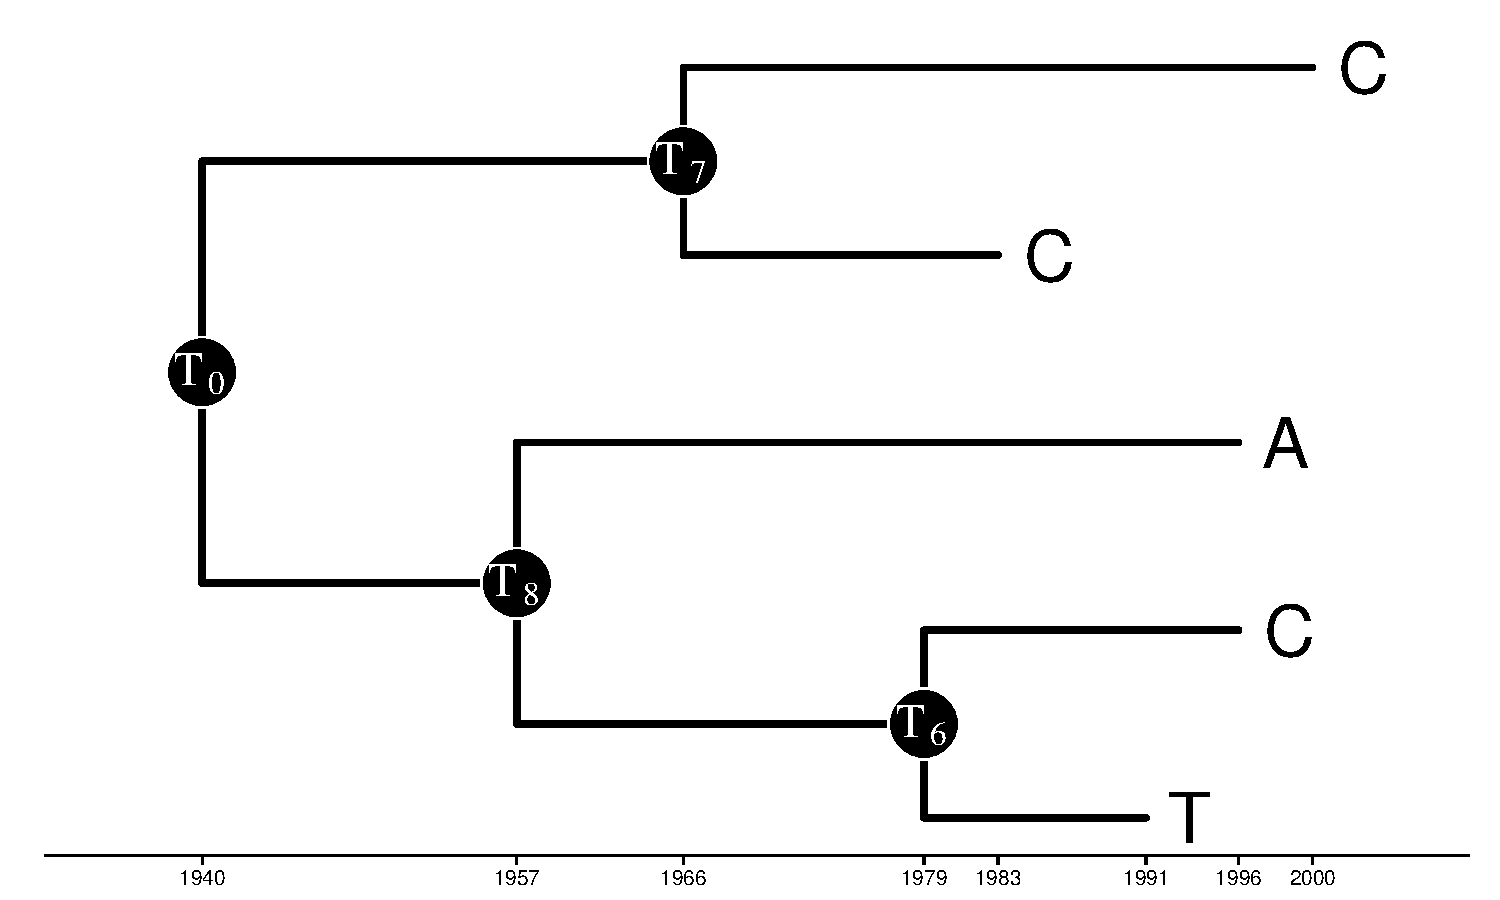
\includegraphics[scale=0.4]{timing_sequences} 
\caption{
{ \footnotesize 
{\bf Dated phylogenetic tree.} 
Discrete characters $CCACT$ observed at the external nodes (the tips of the tree) were sampled at different points in time.
The tree topology is assumed to be known without error, and also the root is known.
The unknown dates of the internal nodes are labelled $T_{0},T_{6},T_{7},T_{8}$.
}% END: footnotesize
}
\label{fig:timing_sequences}
\end{figure}

We start by estimating the rate of mutation $r$, which here is assumed to apply to the whole tree (a strict clock), from the differences in sampling times and the genetic distance, given by the model of sequence substitution.
This allows us to change the scale of the tree from units of substitutions to a time-scale measured in years.
The likelihood of the tree given estimated parameters $r,T_{0},T_{6},T_{7},T_{8}$ can be calculated using methods presented in Subsection~\ref{sub:likelihood}.


\subsection{Sequence evolution on a tree\label{sub:evolutionOnTree}}

In this section we proceed by describing the connection between the CTMC models of character substitution discussed above and phylogenetic histories.
We keep the focus on a single site of the alignment, and due to the assumption of independence the probability of observing an alignment is simply the product of probabilities for observing the individual sites.

To gain a better understanding of the process shaping the data observed at the tips of a phylogenetic tree let us consider the problem of simulating sequence evolution on a tree according to a model with rate matrix $\mathbf{Q}$.
We start with a first character $i$ sampled at the root of the tree $x_0$ from the stationary distribution $\mathbf{\Pi}$.
Let us assume that two direct descendent nodes are $x_j$ and $x_k$.
The character sampled at the root waits an exponentially distributed amount of time $t\geq0$ (see Figure~\ref{fig:poisson}) before moving to one of the descendent or child nodes.
Such traversal is said to be following the pre-order, i.e. parental nodes are visited before child nodes.   
The process then randomly decides by a coin flip to which of the two descendent nodes to move next (assuming that the visited node is not a tip).
Let us assume that the process moved to $x_j$.
The state $j$ for the node $x_j$ is sampled conditional on the value $i$ already sampled at the root using the branch length expressed in real time $t$ and the vector probabilities in the row $i$ of the finite-time probabilities matrix $\mathbf{P}(t)$, calculated using SVD of the rate matrix $\mathbf{Q}$ that characterizes the CTMC.   

\begin{algorithm}[h!]
\centering
\begin{algorithmic}[1]
% \footnotesize{
%
\State $node \gets getRoot\left(\right)$
%
\State $state \gets getState\left(node\right)$
%
\Repeat
%
\If{$\left(hasChildren\left(node\right)\right)$}
%
\ForAll{children}
%
\State $t \gets getDistanceToParent\left(child\right);$
%
\State $ \mathbf{P}\left(t\right) \gets e^{\mathbf{Q}t};$
%
\State $state \gets sample\left(\mathbf{P}\left[ state, \right]\right);$
%
\EndFor
%
\Else \Comment{this is a tip node}
%
\State $node \gets getParent\left(node\right);$
%
\EndIf
%
\Until{$\left(\text{simulated for all nodes}\right)$}
% }
\end{algorithmic}
\caption{
{ \footnotesize 
{\bf Pseudo code for simulating an evolutionary process along a phylogeny.} 
When a child node is visited, the state is sampled with conditional probabilities of changing to state $j$ given state $i$ at the parental node.
}% END: footnotesize
}
\label{alg:simulation}
\end{algorithm}

This illustrates the Markov property of a CTMC, as defined in Equation~(\ref{eq:markov}).
The sampling is then repeated on the node $x_j$, before recursively proceeding to the other trio of nodes.
The states sampled at the tips of the tree constitute the character sequence for one site of the alignment.
In this light the CTMC process can be viewed as a continuous-time random walk, unfolding on the topology $\mathbf{F}$, with its behaviour described by a rate-matrix $\mathbf{Q}$.
The complete algorithm is listed in Algorithm~\ref{alg:simulation}.

\section{Likelihood of sequence evolution}

\subsection{Calculation of the likelihood on a tree\label{sub:likelihood}}

The likelihood is defined as a conditional probability of observing the data given the parameters, as a function of those parameters.
%PL: mention perhaps Fisher, Edwards..?
Phylogenetic inference considers discrete molecular sequence data in the form of an aligned matrix $\mathbf{X}$ of size $n \times l$, where $x_{jh}$ is the $h$-th character in the $j$-th sequence.
A single column $\mathbf{x}_{h}$ of the data matrix constitutes a single site.
Again, the standard assumption of (site and lineage) independence posits that different sites evolve independently and that once two branches split at a node, the evolution on those branches is also independent.

In Subsection~\ref{sub:evolutionOnTree}, we described how evolution according to some process $\mathbf{Q}$ gives rise to the observed data $\mathbf{X}$.
Typically, we start with just the observed data and aim the inference efforts at modeling the process that generated the alignment.
We can therefore denote the likelihood simply as: 

\begin{equation}
L\left(\mathbf{\Theta}|\mathbf{X}\right)=P\left( \mathbf{X} | \mathbf{\Theta} \right), 
\label{eq:likelihood}
\end{equation}

\noindent
where $\mathbf{\Theta}$ represents the tree topology, the branch lengths, the parameters of the substitution model and other parameters of interest that we want to estimate.
This quantity expresses how likely it is to observe the data given a specific value of the parameter(s) of interest $\mathbf{\Theta}$.
\myedit{sveight}{
By finding the value of $\mathbf{\Theta}$ that maximizes (\ref{eq:likelihood}) we obtain an estimate of the most plausible 
%hypothesis for the data.
set of parameters given the observed data.}

In this thesis we will not discuss maximum likelihood estimation itself, %PL: good, who wants to consider the data to be fixed anyway..
rather focus on closely related 
%PL: I would add: ".., but philosophically very different,"
% FB: difference: ML is an optimization procedure, Bayesian inference is a conditioning. It's a less aggresivee approach 
methods of Bayesian inference.
%GB: 'enters the framework as the data component' ? sounds weird, please rephrase
The likelihood concept is also required in Bayesian inference and enters the framework as the data component.
We will now discuss how to calculate the likelihood of observing a particular realization of character sequences at the tips of a tree, given a substitution model with fixed parameters.

%---LIKELIHOOD---%
\begin{figure}[h!]
\centering
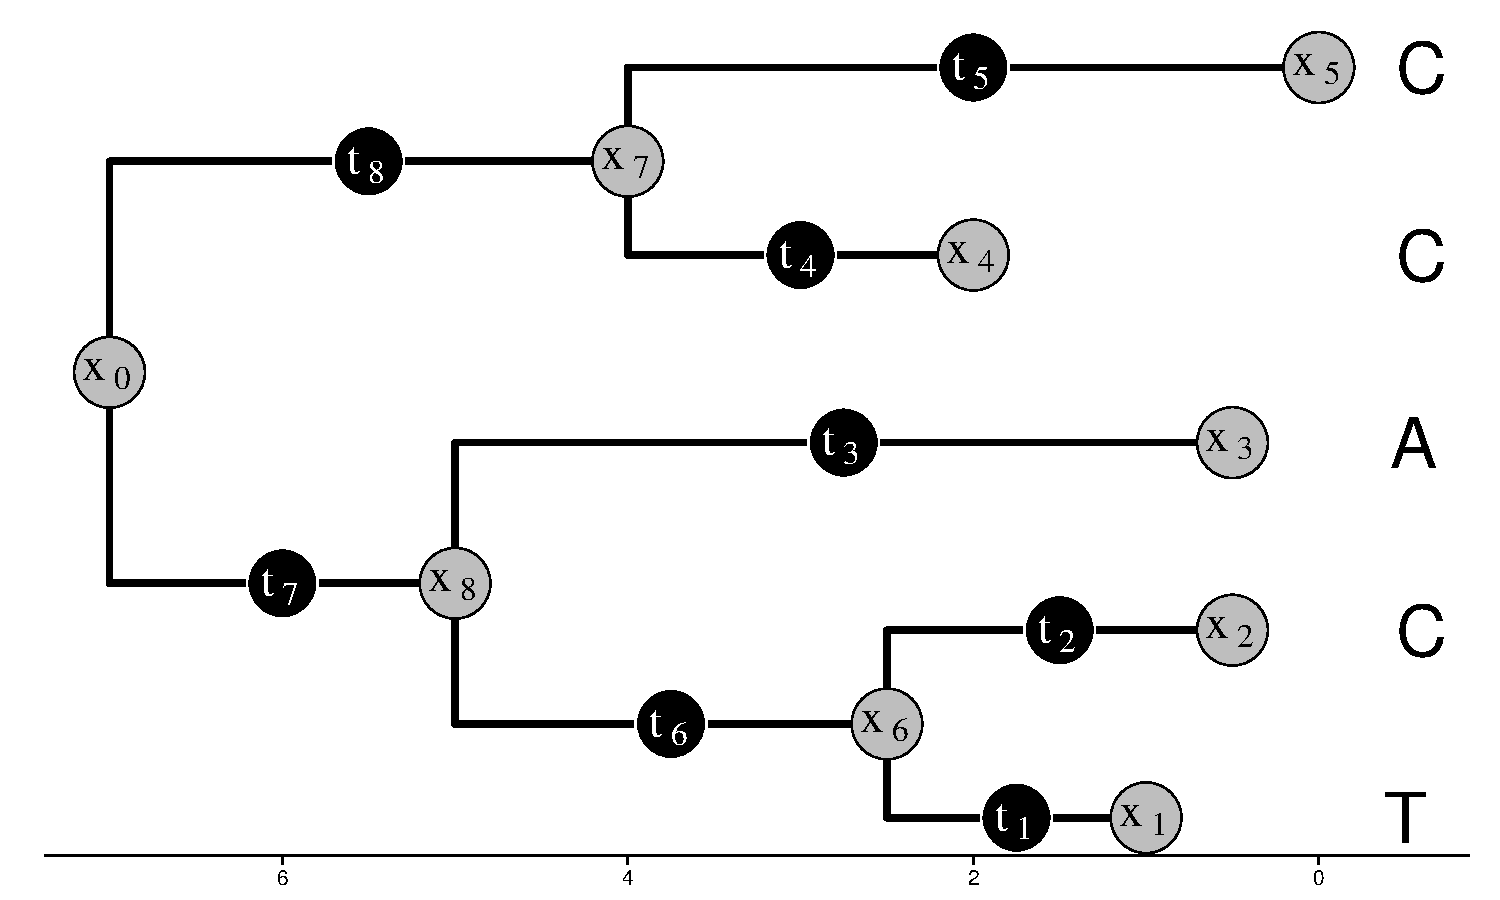
\includegraphics[scale=0.4]{likelihood} 
\caption{
{ \footnotesize 
{\bf  A hypothetical tree for five taxa.} Character data for a single site is observed at the tips of the tree.
} % END: footnotesize
}
\label{fig:LIKELIHOOD}
\end{figure}

To calculate the likelihood means in a sense to reverse-engineer the evolution as it happened.
Figure~\ref{fig:LIKELIHOOD} presents a single site with data $TCACC$ observed at the tips of the tree.
External nodes are numbered $x_{1}, \ldots x_{5}$, internal nodes $x_{6}, \ldots x_{8}$ and the root is placed at the node $x_{0}$.
The length of each branch leading to node $i$ is denoted as $t_{i}$. 
Using the methods presented in Subsection~\ref{sub:exponentiation}, we calculate the finite-time transition probabilities $p_{ij}(t_{i})$ between all pairs of characters in the alignment.
To calculate the probability at a single site, we need to sum over all possible combinations that could give rise to the observed character data at that site, in this case:

\begin{align}
\underset{x_{0}\in \mathcal{E}}{\sum}\;\underset{x_{6}\in \mathcal{E}}{\sum}\;\underset{x_{7}\in \mathcal{E}}{\sum}\;\underset{x_{8}\in \mathcal{E}}{\sum}[\pi_{x_{0}}\cdot p_{x_{0}x_{8}}(t_{7})\cdot p_{x_{0}x_{7}}(t_{8})\cdot p_{x_{8}x_{6}}(t_{6})\cdot p_{x_{8}A}(t_{3}) \nonumber \\
\cdot p_{x_{7}C}(t_{4})\cdot p_{x_{7}C}(t_{5})\cdot p_{x_{6}T}(t_{1})\cdot p_{x_{6}C}(t_{2})].
\label{eq:likelihoodNaive}
\end{align}

We can break down the terms in Equation~(\ref{eq:likelihoodNaive}) 
to the probability of observing the data $TCACC$ for the tips and $x_{0},x_{6},x_{7},x_{8}$ for the ancestral nodes (inside the brackets) and the sum over all possible path combinations over the state space $\mathcal{E}$ (outside the brackets).
Term $\pi_{0}$ is simply the probability that the root has character $x_{0}$ and is based on the assumption that the process generating the data has reached its equilibrium.

Summing over all possible paths leading to the observed data is computationally expensive, as there are  $K^{n-1}$ possible combinations, where $n-1$ is the number of internal nodes of a rooted binary tree.
Fortunately, we can rely on the assumption of independence of the process in the two sub-trees below every node.
Based on this, \citet{Felsenstein1981} provides an efficient algorithm for computing the likelihood of observing the data on a topology $\mathbf{F}$ given the substitution model that quantifies transition probabilities.
This routine, known as \emph{tree pruning}, conveniently expresses the partial likelihood $L_{i}(x_{i})$ of observing data at the descendants of node $i$ given state $x_{i}$ at node $i$ in terms of partial likelihoods at nodes $j$ and $k$.
For all internal nodes of $\mathbf{F}$ we have:

\begin{equation}
L_{i}(x_{i})=\left[\underset{x_{j}\in \mathcal{E}}{\sum}\mathbf{P}_{x_{i}x_{j}}(t_{j})L_{j}(x_{j})\right]\times\left[\underset{x_{k}\in \mathcal{E}}{\sum}\mathbf{P}_{x_{i}x_{k}}(t_{k})L_{k}(x_{k})\right]
\label{eq:felsenstein1}
\end{equation}

\noindent
For tip nodes we have:

\begin{equation}
L_{i}(x_{i})=\begin{cases}
1 & \text{if }\hat{x}(i)=x_{i}\\
0 & \text{otherwise}
\end{cases},
\label{eq:felsenstein2}
\end{equation}

\noindent
where $\hat{x}(i)$ denotes the character state observed at node $i$.
After recursively applying (\ref{eq:felsenstein1}) to all the nodes of $\mathbf{F}$ in post-order fashion, the likelihood of the data at the site is given by:
% we can integrate out the unobserved states calculating successive contributions to the partial likelihood.

\begin{equation}
L(\mathbf{x}_{h})=\underset{x_{0}\in\mathcal{E}}{\sum}\pi_{x_{0}}\cdot L_{0}(x_{0})
\label{eq:felsenstein3}
\end{equation}

\noindent
In most applications for computational reasons is is easier to work with the natural logarithm of the likelihood in Equation~\ref{eq:felsenstein3}.
Thanks to the assumption of site-independence, the log-likelihood of the whole alignment $X$ can be computed by summing the logarithms of the likelihoods at the particular sites:

\begin{equation}
l(X)=\underset{j=1}{\overset{l}{\sum}}log\left(L(\mathbf{x}_{jh})\right)
\label{eq:loglikelihood}
\end{equation}

\subsection{The computational burden of likelihood computations\label{sub:mlburden}}

We have already mentioned that for large data sets the run-time of statistical phylogenetic analysis is a major hurdle that hampers the development and application of novel, more biologically relevant models and inference in the field.
These limits are being actively stretched, for example by porting the computationally expensive calculations to high-performance parallel computing devices such as Graphics-Processing Units (GPUs, \cite{Nickolls2008}).
In Subsection~\ref{sub:exponentiation}, we already discussed how the computation of finite-time transition probabilities can be reduced to simple matrix algebra operations, which can be handled by high-performance libraries and APIs for statistical phylogenetics such as the BEAGLE library \citep{Ayres2012, Suchard2009}. 

Before we proceed with discussing the burden imposed by certain steps when calculating the likelihood of a sequence evolution on a tree, we need a formal definition of the computational complexity of a sequential routine.
The efficiency of an algorithm can depend on various factors, like network usage, disk usage, operational memory usage or CPU real-time usage.
All of these factors should be taken into consideration when designing and implementing a computational routine. 
However, for most of the calculations the CPU time will be the rate-limiting factor.
Typically both mathematicians and computer scientists use the Big-O notation as a relative representation of algorithm complexity, like the execution time required.
Here we formally define the Big-O notation as:

\begin{definition}
Let us assume two functions $f:\mathbb{R}_{>0}\rightarrow\mathbb{R}_{>0}$ and $T:\mathbb{R}_{>0}\rightarrow\mathbb{R}_{>0}$. 
For $n \in \mathbb{R}_{>0}$ we write:

\begin{equation}
T(n) \in \mathcal{O}\left(f(n)\right)
\label{eq:bigOh}
\end{equation}

\noindent
if and only if there exists a constant $M>0$ and some $n_0 \in \mathbb{R}_{>0}$ such that:

\begin{equation}
\forall n\geq n_{0}\;T(n)\leq M \cdot f(n)
\end{equation}
\end{definition}


% \noindent
In other words $T(n)$, which can be interpreted as the ``worst-case'' time complexity of an algorithm,
% Since an algorithm's performance time may vary with different inputs of the same size
is $\mathcal{O}\left(f(n)\right)$ if and only if for all sufficiently large input values $T(n)$ is bounded from above by some constant multiple of $f(n)$.
This makes the Big-O notation useful when analyzing algorithms for run-time efficiency and makes it possible to, for example, compare routines without the added overhead of negligible terms, such as the architecture at which the code was run, the choice of language or compiler.
We will now briefly discuss some of the most common serial computational orders and their examples. 

\begin{algorithm}[h!]
\centering
\begin{algorithmic}[1]
% \footnotesize{
\State $a \gets \text{\textbf{new int}}$;
%
\If{ $\left(a == 1 \right)$ }
%
\State \textbf{return} $true$;
%
\Else 
%
\State \textbf{return} $false$;
%
\EndIf
% }
\end{algorithmic}
\caption{
{ \footnotesize 
{\bf Single test operation.} 
} % END: footnotesize
}
\label{alg:o1}
\end{algorithm}

The simplest, most basic example is an operation that takes the same amount of time every time it is called, thus requiring constant time, i.e. it's computational complexity is that of $\mathcal{O}\left(1\right)$ and does not depend on the input size.
An example of such routine is listed in the Algorithm~\ref{alg:o1} that evaluates a specific value of a constant.

\begin{algorithm}[h!]
\centering
\begin{algorithmic}[1]
% \footnotesize{
\State $a \gets \text{\textbf{new int}}\left[n\right]$;
%
\For{int $\left(i=0; \; i<a.size(); \; i++\right)$}
%
\If{ $\left(a\left[i\right] == 1 \right)$ }
%
\State \textbf{return} $true$;
%
\Else 
%
\State \textbf{return} $false$;
%
\EndIf
%
\EndFor
% }
\end{algorithmic}
\caption{
{ \footnotesize 
{\bf Search for a value.} 
}% END: footnotesize
}
\label{alg:on}
\end{algorithm}

An algorithm proceeding at $\mathcal{O}\left(N\right)$ has a run-time that grows linearly with the size of input data.
An example of such a routine is presented as Algorithm~\ref{alg:on}, which searches an array looking for a specific value.
We should note that the Big-O notation always describes the performance in worst-case scenario, i.e. a full loop has to be executed before a matching element is found, while for the actual real-world problem this does not have to be the case and the loop can return earlier.

\begin{algorithm}[h!]
\centering
\begin{algorithmic}[1]
% \footnotesize{
\State $a \gets \text{\textbf{new int}}\left[n\right]$;
%
\For{int $\left(i=0; \; i<a.size(); \; i++\right)$}
%
\For{int $\left(j=0; \; j<a.size(); \; j++\right)$}
%
\If{ $\left(i == j \right)$ }
%
\State \textbf{do nothing};
%
\Else 
%
\If{ $a\left[ i \right] == a\left[ j \right]$ }
%
\State \textbf{return} $true$;
%
\EndIf
%
\EndIf \Comment{END: i == j check}
%
\EndFor \Comment{END: j loop}
%
\EndFor \Comment{END: i loop}
% }
\end{algorithmic}
\caption{
{ \footnotesize 
{\bf Search for the first duplicated value.} 
}% END: footnotesize
}
\label{alg:on2}
\end{algorithm}

An algorithm can also require a quadratic run-time, $\mathcal{O}\left(N^2\right)$, i.e. its performance is directly proportional to the square of the size of the input data.
Among examples of such an algorithm is the routine that searches for a duplicated value in an array, and requires two nested loops as presented in Algorithm~\ref{alg:on2}.
Similarly, nesting more loops will result in routines which proceed at polynomial times $\mathcal{O}\left(N^3\right)$, $\mathcal{O}\left(N^4\right)$, $\mathcal{O}\left(N^5\right)$, etc.
An algorithm proceeding at $\mathcal{O}\left(c^N\right)$, where $c>1$ is some constant, will have a run-time that grows c-times with every additional data element, i.e. exponentially. 

Having described these basic concepts, we can now come back to the original problem of calculating the likelihood of sequence evolution on a fixed tree.
From Subsections \ref{sub:exponentiation} and \ref{sub:likelihood} we already know the steps involved:

% I skipped site rate variability, but perhaps it should be mentioned? 
\begin{enumerate}
\item { Singular value decomposition of the rate matrix $\mathbf{Q}$. }
\item { Taking the exponential of $\mathbf{Q}t$ for each branch length $t$. }
\item { Applying Equation~(\ref{eq:felsenstein1}) for every site in the alignment and every possible state in the state space $\mathcal{E}$. }
\item { Taking the logarithm of the likelihood for every site and summing over all sites in the alignment. }
\end{enumerate}

Step (i) proceeds at ${\cal{O}}(K^3)$; however, for typical, time-homogeneous applications this is not the rate-limiting step, as repeated evaluations of $\exp(\mathbf{Q}t)$ in (ii) are based on the same decomposition of the matrix \citep{Suchard2009}. 
Step (ii) typically boils down to repeated matrix-vector-matrix multiplications and its serial computational order is ${\cal{O}}(K^3 \times n)$. 
Step (iii) takes ${\cal{O}}(K^2 \times n \times l)$ time and is the most computationally expensive part of the routine. 
Step (iv) proceeds at ${\cal{O}}(l)$, linearly with the number of sites.
Fortunately, these operations are very regular and lend themselves to exploit computational parallelism, such as utilized in the BEAGLE library \citep{Suchard2009,Ayres2012}.

% TODO: maybe sub-section on GPUs here

\section{Bayesian inference\label{sec:bayesian_inference}}

\subsection{Bayesian evolutionary analysis}

The Bayesian approach to statistical inference combines prior information with the data to generate the posterior distributions of the parameters of interest.
All other post-hoc inference is based on those generated posterior distributions.
Bayesian methodology has recently gained immense popularity, due to the advances in numerical algorithms and the progressively cheaper access to powerful computational hardware.
The development of statistical programs for simulation from Bayesian hierarchical models like OpenBUGS \citep{Lunn2009} and JAGS \citep{Plummer2003} has also helped to bolster the popularity and accessibility of the Bayesian framework.

In the field of phylogenetics, Bayesian inference has been applied to some of the most complex problems and is now widely adopted, with the term \emph{Bayesian evolutionary analysis} used to describe molecular evolutionary analyses set in the Bayesian framework.
At the forefront of these advancements lies the active development and wide adoption of popular Bayesian evolutionary analysis software packages like MrBayes \citep{Ronquist2012} and BEAST \citep{Drummond2012}.

\subsection{Bayes theorem\label{sub:bayesTheorem}}

% Following the notation defined in Subsection \ref{sub:likelihood} we will denote the tree topology, the branch lengths and the parameters of the substitution model that we aim at inferring by $\mathbf{\Theta}$.
Following the notation defined in Subsection~\ref{sub:likelihood}, let us denote a single-dimensional parameter of interest that we aim to learn about as $\theta$.
The central concept of Bayesian inference is that this parameter has a distribution of its own.
Before the molecular data $\mathbf{X}$ is observed we assume that $\theta$ has a prior distribution $P(\theta)$.
The prior reflects the prior beliefs about the possible values of the parameter.

\myedit{svnine}{
The prior choice is perhaps one of the most controversial aspects of the Bayesian inference.
The prior distributions may be inspired by previous analyses of other sets of data, or they may form some set of biologically plausible values.
However in some cases there may be no suitable objective prior knowledge at hand, in which case one often resorts to the so-called \emph{vague} or \emph{diffuse} priors, which have large variances.
Some popular uninformative priors on continuous, unbounded variables may be improper, \textit{i.e.} their distribution is infinitesimal on an infinite range in order to integrate to $1$.
Among examples of such priors is the uniform distribution on an infinite interval.
Although many of these prior choices still lead to a proper posterior distribution, some controversies about their choice may still arise, in particular when the data is poorly informative.
}

% TODO: discuss hyperpriors?
The prior information is then combined with the likelihood of the data $P\left( \mathbf{X} | \theta \right)$ to form the posterior, via Bayes' theorem (Equation~(\ref{eq:bayesian1})).
The posterior distribution of $\theta$ follows:

\begin{align}
P\left(\theta|\mathbf{X}\right) &= \frac{P(\theta)\cdot P\left(\mathbf{X}|\theta\right)}{P\left(\mathbf{X}\right)}=\frac{P(\theta)\cdot P\left(\mathbf{X}|\theta\right)}{\int P(\theta)\cdot P\left(\mathbf{X}|\theta\right)d\theta}  \nonumber \\
& \approx  P(\theta)\cdot P\left(\mathbf{X}|\theta\right),
\label{eq:bayesian1}
\end{align}

\noindent
where the marginal probability of the data $P\left(\mathbf{X}\right)$ is a normalizing constant that makes the posterior $P\left(\theta|\mathbf{X}\right)$ integrate to one.
The last approximation in Equation~(\ref{eq:bayesian1}) means that the posterior is proportional to the prior times the likelihood.

% nuisance parameters? GB: I second that
Bayesian inference provides a natural way of dealing with nuisance parameters.
Suppose that $\mathbf{\Theta}=\left(\theta,\mathbf{F}\right)$ is now a two dimensional vector of parameters, with $\theta$ being the parameter of interest, while 
$\mathbf{F}$ (e.g. a tree topology) is the nuisance parameter.
The joint posterior distribution of $\mathbf{\Theta}$ is now:

\begin{eqnarray}
P\left(\mathbf{\Theta}|\mathbf{X}\right) &=& P\left(\theta,\mathbf{F}|\mathbf{X}\right)=\frac{P\left(\theta,\mathbf{F}\right)\cdot P\left(\mathbf{X}|\theta,\mathbf{F}\right)}{P\left(\mathbf{X}\right)}  \nonumber \\
&=& \frac{P\left(\theta,\mathbf{F}\right)\cdot P\left(\mathbf{X}|\theta,\mathbf{F}\right)}{\int\int P(\theta,\mathbf{F})\cdot P\left(\mathbf{X}|\theta,\mathbf{F}\right)d\theta d\mathbf{F}}
\label{eq:bayesian2}
\end{eqnarray}

\noindent
and the marginal posterior density of $\theta$ can be obtained from Equation~\ref{eq:bayesian2} as:

\begin{equation}
P\left(\theta|\mathbf{X}\right) =\int P\left(\theta,\mathbf{F}|\mathbf{X}\right)d\mathbf{F}
\label{eq:bayesian3}
\end{equation}

\subsection{Example: Comparing two sequences with the beta-binomial model\label{sub:ex_beta_binom}}

As a simple illustration of the concept of Bayesian analysis, let us consider a toy example where two sequences are compared and $x=10$ differences are found out of $N=100$ sites compared.
Suppose that the parameter $\theta$ we want to infer is the proportion of sites which differ between the two sequences.
Assuming that the sites are independent we can use a binomial model and put a beta prior with parameters $\alpha=2$, $\beta=100$ on the unknown proportion $\theta$, suggesting that \textit{a priori} we prefer small values of the $\theta$ parameter.


%---POSTERIOR PRIOR LIKELIHOOD---%
\begin{figure}[h!]
\centering
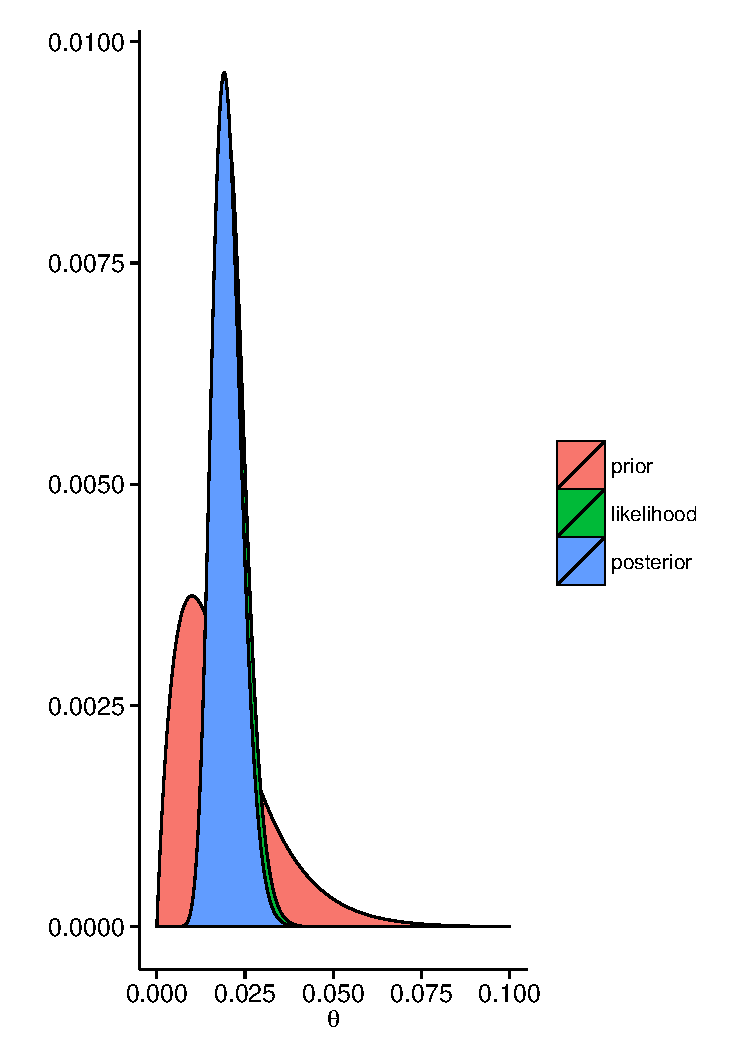
\includegraphics[scale=0.45]{bayes} 
\caption{
{ \footnotesize 
{\bf Beta(2,100) prior and posterior densities plotted with a scaled likelihood resulting from a binomial model.} 
}% END: footnotesize
}
\label{fig:bayes1}
\end{figure}

\myedit{sveleven}{
Figure~\ref{fig:bayes1} shows the resulting posterior distribution along with the prior and the scaled likelihood.
The likelihood of the binomial model used in this example is simply:
}

\begin{align}
L\left(\theta|x\right)=\left(\begin{array}{c}
N\\
x
\end{array}\right)\theta^{x}(1-\theta)^{N-x}
\label{eq:binomial_like}
\end{align}

Equation~\ref{eq:binomial_like} is plotted in Figure~\ref{fig:bayes1} over a range of values of $\theta$, resulting in the black filled distribution.
The Beta distribution we choose for the prior has a following distribution function:

\begin{align}
p(\theta)=\frac{1}{B\left(\alpha,\beta\right)}\theta^{\alpha-1}(1-\alpha)^{\beta-1}
\label{eq:beta_dist}
\end{align}

Equation~\ref{eq:beta_dist} corresponds to the white filled curve in in Figure~\ref{fig:bayes1}.
Following the Bayes rule from Equation~\ref{eq:bayesian1}, we can combine the likelihood and prior to arrive at the posterior, which then becomes:

\begin{eqnarray}
p\left(\theta|x\right)=& \frac{\left(\begin{array}{c}
N\\
x
\end{array}\right)\theta^{x}(1-\theta)^{N-x}\times\frac{1}{B\left(\alpha,\beta\right)}\theta^{\alpha-1}\left(1-\theta\right)^{\beta-1}}{\int\left(\begin{array}{c}
N\\
x
\end{array}\right)\theta^{x}(1-\theta)^{N-x}\times\frac{1}{B\left(\alpha,\beta\right)}\theta^{\alpha-1}\left(1-\theta\right)^{\beta-1}d\theta} \nonumber \\
=& \frac{1}{B\left(\alpha+x,\beta+N-x\right)}\theta^{\alpha+x-1}(1-\theta)^{\beta+N-x-1}
\label{eq:beta_binom_post}
\end{eqnarray}
 
Equation~\ref{eq:beta_binom_post} appears as a grey filled area in Figure~\ref{fig:bayes1}.
This illustrates that the data `pulls' the posterior away from the prior, and the strength by which is does so depends on its variance, resulting in a posterior centred around 0.06 in this case.
In this example, the posterior distribution can be obtained analytically because the beta distribution is a so-called \emph{conjugate prior} for the binomial model, resulting in the posterior that is also beta-distributed.


\subsection{Markov Chain Monte Carlo\label{sub:mcmc} }

Except for the most trivial problems, involving conjugate priors as in our previous example, the calculation of the integral in Equation~(\ref{eq:bayesian1}) poses a considerable challenge in Bayesian inference.
This integral leads to the marginal probability of the data $P\left(\mathbf{X}\right)$. 
For even the simplest phylogenetic problems, one has to integrate over all possible tree topologies, all of the branch lengths in those trees and all of the substitution parameters in the applied model.
Such highly-dimensional integrals are impossible to calculate analytically.
This is where the Markov Chain Monte Carlo (MCMC) algorithm shows its strength and provides a powerful method of sampling from the posterior distributions without having to evaluate the marginal probability. %PL: it is a supa-dupa algorithm: http://oldweb.cecm.sfu.ca/~jborwein/algorithms.html

The Metropolis-Hasting algorithm, as proposed by \citet{Metropolis1953}, is an MCMC algorithm for sampling from multi-dimensional distributions.
It proceeds by constructing a Markov chain with its states being the values of the parameter of interest $\theta$ and whose equilibrium distribution is the posterior $P\left(\theta|\mathbf{X}\right)$ as defined in Equation~\ref{eq:bayesian1}.
After choosing an arbitrary starting state for the chain, new candidate states $\theta^{*}$ are generated from the proposal density, also called the kernel, $q(\theta^{*} | \theta[t]), \; t=1,\ldots,M$, where $M$ is the chain length and $\theta[t]$ is the current value of the chain.

A common kernel choice to propose new state for continuous parameter is to sample from a uniform distribution centered around the current state of the chain, the so-called sliding window kernel: 

$$\theta^{*}\sim U\left[\theta[t]-\omega,\theta[t]+\omega\right], \; t=1,\ldots,M,$$

\noindent
where $\omega$ is the arbitrary window size.
The chain then moves to the proposed value with probability defined by the acceptance ratio (see Equation~(\ref{eq:metropolis1})), or if the proposal is rejected the chain remains at the current state.
The routine iterates between accept/reject steps for a specified number of times.
Both acceptance and rejection are counted as iterations of the algorithm; in fact the rejections ensure that the probabilistic properties of the target distribution are well represented in the generated sample.  
Algorithm~\ref{alg:metropolisHastings} presents the details of the Metropolis-Hastings algorithm.

\begin{algorithm}[h!]
\centering
\begin{algorithmic}[1]
% \footnotesize{
%
\State Pick a starting value of the chain $\theta \left[ t \right]$ for $t=0$.
%
\For{int $\left(t=1; \; t<M-1; \; t++\right)$}
%
\State Generate a candidate state from the proposal distribution (kernel):
$$\theta^{*} \sim q(\theta[t])$$
%
\State Calculate the acceptance ratio:
$$r=\frac{prior\left(\theta^{*}\right)}{prior\left(\theta\left[t\right]\right)}\cdot\frac{Likelihood\left(\mathbf{X}|\theta^{*}\right)}{Likelihood\left(\mathbf{X}|\theta\left[t\right]\right)}\cdot\frac{q\left(\theta\left[t\right]|\theta^{*}\right)}{q\left(\theta^{*}|\theta\left[t\right]\right)}.$$
%
\State Sample $u\sim U[0,1]$.
%
\If{$\left( u < r \right)$}
%
\State Set $\theta[t+1]=\theta^*.$
%
\Else 
%
\State Set $\theta[t+1]=\theta[t].$
%
\EndIf
%
\EndFor
% }
\end{algorithmic}
\caption{
{ \footnotesize 
{\bf The Metropolis-Hastings algorithm} 
}% END: footnotesize
}
\label{alg:metropolisHastings}
\end{algorithm}

Several important features of the algorithm can be noted.
The most important part of the algorithm is the proposal density. 
Given the current state it proposes the next state independent of the past states.
We can recall that this is the Markov property, in fact the output of the algorithm generates a Markov chain, hence the name MCMC.
The Metropolis-Hastings algorithm allows for the use of an asymmetrical proposal densities such that $q\left(\theta\left[t\right]|\theta^{*}\right)\neq q\left(\theta^{*}|\theta\left[t\right]\right)$.
The acceptance probability is simply the ratio of the target posterior evaluated at the proposal and at the current state of the chain, times the ratio of the proposal: 
% prior ratio times the likelihood ratio times the proposal ratio

% \myedit{DPseven}{
\begin{equation}
\frac{P\left(\theta^{*}|\mathbf{X}\right)\cdot q\left(\theta\left[t\right]|\theta^{*}\right)}{P\left(\theta\left[t\right]|\mathbf{X}\right)\cdot q\left(\theta^{*}|\theta\left[t\right]\right)}=\frac{P(\theta^{*})\cdot P\left(\mathbf{X}|\theta^{*}\right)\cdot q\left(\theta\left[t\right]|\theta^{*}\right)}{P(\theta\left[t\right])\cdot P\left(\mathbf{X}|\theta\left[t\right]\right)\cdot q\left(\theta^{*}|\theta\left[t\right]\right)}.
\label{eq:metropolis1}
\end{equation}
% }

Note that the integral in Equation~(\ref{eq:bayesian1}) which is notoriously hard to compute cancels out in (\ref{eq:metropolis1}).
Hence, to estimate the posterior $P\left(\theta|\mathbf{X}\right)$ one only needs to run the algorithm for a sufficiently long time to let the chain reach its equilibrium, which is precisely the target posterior.
%PL: maybe mention that this can be formally proven using the ergodic theorem... and no, you don't have to prove it in the appendix ;-)

\subsection{Example: Estimating genetic distances}

Let us revisit the toy example in which we compare two sequences and find $x=10$ differences among $n=100$ sites.
This time however we will use MCMC to estimate the genetic distance between the two sequences using the Jukes and Cantor model of nucleotide substitution (see Subsection~\ref{sub:jc69}).
Genetic distance is defined as the expected number of substitutions per nucleotide site, which we will denote as $\theta=rt$ in line with previous sections, where $r$ is the substitution rate (see Subsection~\ref{sub:poisson}) and $t$ is the evolutionary time separating the two sequences.
The time and rate are generally confounded as we already mentioned, and hence they will be estimated as a single parameter of interest $\theta$.
The probability that the descendant nucleotide in a sequence is different from the ancestral nucleotide can be obtained by summing over all possible paths, between two pairs of nucleotides, i.e. $p_{ij}(t)=\underset{k\neq i}{\sum}p_{ik}(t)$.

From Equation~(\ref{eq:jc69Finite}) in Subsection~\ref{sub:jc69}, we know that under the JC69 model those probabilities are all equal, therefore the probability that a single site is different between two sequences separated by distance $\theta=rt$ is given by:

\begin{equation}
p=3p_{1}\left(t\right)=\frac{3}{4}\left(1-e^{\left(-4/3\right)\theta}\right).
\label{eq:distance1}
\end{equation}

\noindent
From this we can formalize the likelihood function using the binomial model given that we observe $x$ differences out of $n$ sites :

\begin{equation}
P\left(\mathbf{X}|\theta\right)=L\left(\mathbf{X}|\theta\right)=\left(\begin{array}{c}
n\\
k
\end{array}\right)p^{x}(1-p)^{n-x},
\label{eq:likelihood1}
\end{equation}

\noindent
where $p$ is as defined by Equation~(\ref{eq:distance1}).
We use an exponential prior on $\theta$ with mean $1/\lambda$:

\begin{equation}
P\left(\theta,\lambda\right)=\frac{1}{\lambda}e^{-(1/\lambda)\theta},
\label{eq:expPrior}
\end{equation}

\noindent
and set $\lambda=10$.
For the proposal we choose a uniformly distributed jumping kernel with a window size of $w=0.1$.

%---METROPOLIS PATH---%
\begin{figure}[h!]
\centering
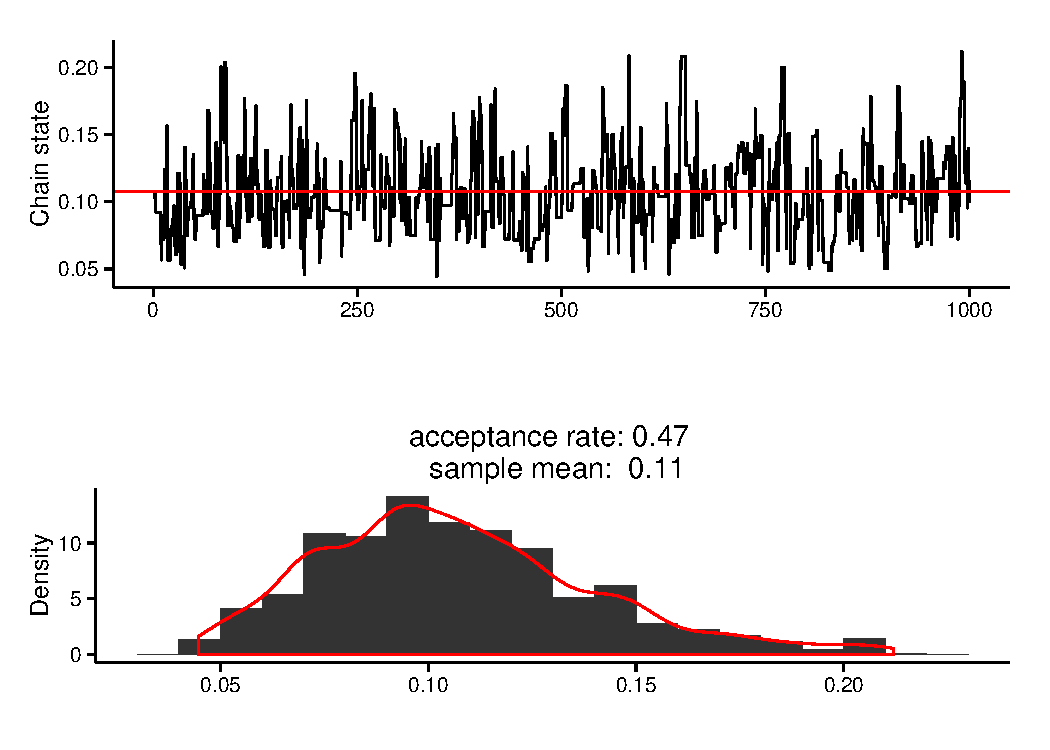
\includegraphics[scale=0.5]{metropolis} 
\caption{
{ \footnotesize 
{\bf MCMC output for estimating the genetic distance under the JC69 model.}
Trace plot in the upper panel results from a direct implementation of Algorithm~\ref{alg:metropolisHastings}.
The likelihood is calculated under the binomial model, with probabilities coming from the JC69 nucleotide substitution model. 
We put an exponential prior on the parameter $\theta$.
With the grey line we indicate the MLE estimator of $\theta$. 
In the lower panel we plot the posterior density estimated using MCMC.
}% END: footnotesize
}
\label{fig:metropolis}
\end{figure}

Figure~\ref{fig:metropolis} shows $1000$ iterations of the chain generated by Algorithm~\ref{alg:metropolisHastings} in the upper plot and applied to the genetic distance problem.
The grey line indicates the maximum likelihood estimate (MLE) $\hat{\theta}$ of parameter $\theta$ which is calculated by setting $\frac{d\ell\left(\mathbf{X}|\theta\right)}{d\theta}=0$, where $l\left(\mathbf{X}|\theta\right)$ is the logarithm of likelihood defined by Equation~(\ref{eq:likelihood1}):

\begin{equation}
\hat{\theta}=\frac{3}{4}log\left(1-\frac{4}{3}\cdot\frac{x}{n}\right)
\label{eq:mle}
\end{equation}

In the lower plot of Figure~\ref{fig:metropolis} we can see an estimate of the posterior density, along with the sample mean.
The posterior sample mean is identical to the MLE up to the second decimal place, although we have not run the chain for long.
The acceptance rate is high, suggesting that almost as many steps are accepted as are rejected.
%GB: acceptance rates don't necessarily have to be this high, not sure if you want to discuss this though.

For reference we now repeat the same procedure, yet this time we set the window size to $w=1.0$.
The resulting time-series plot is presented in Figure~\ref{fig:window_size}.

%---WINDOW SIZE---%
\begin{figure}[h!]
\centering
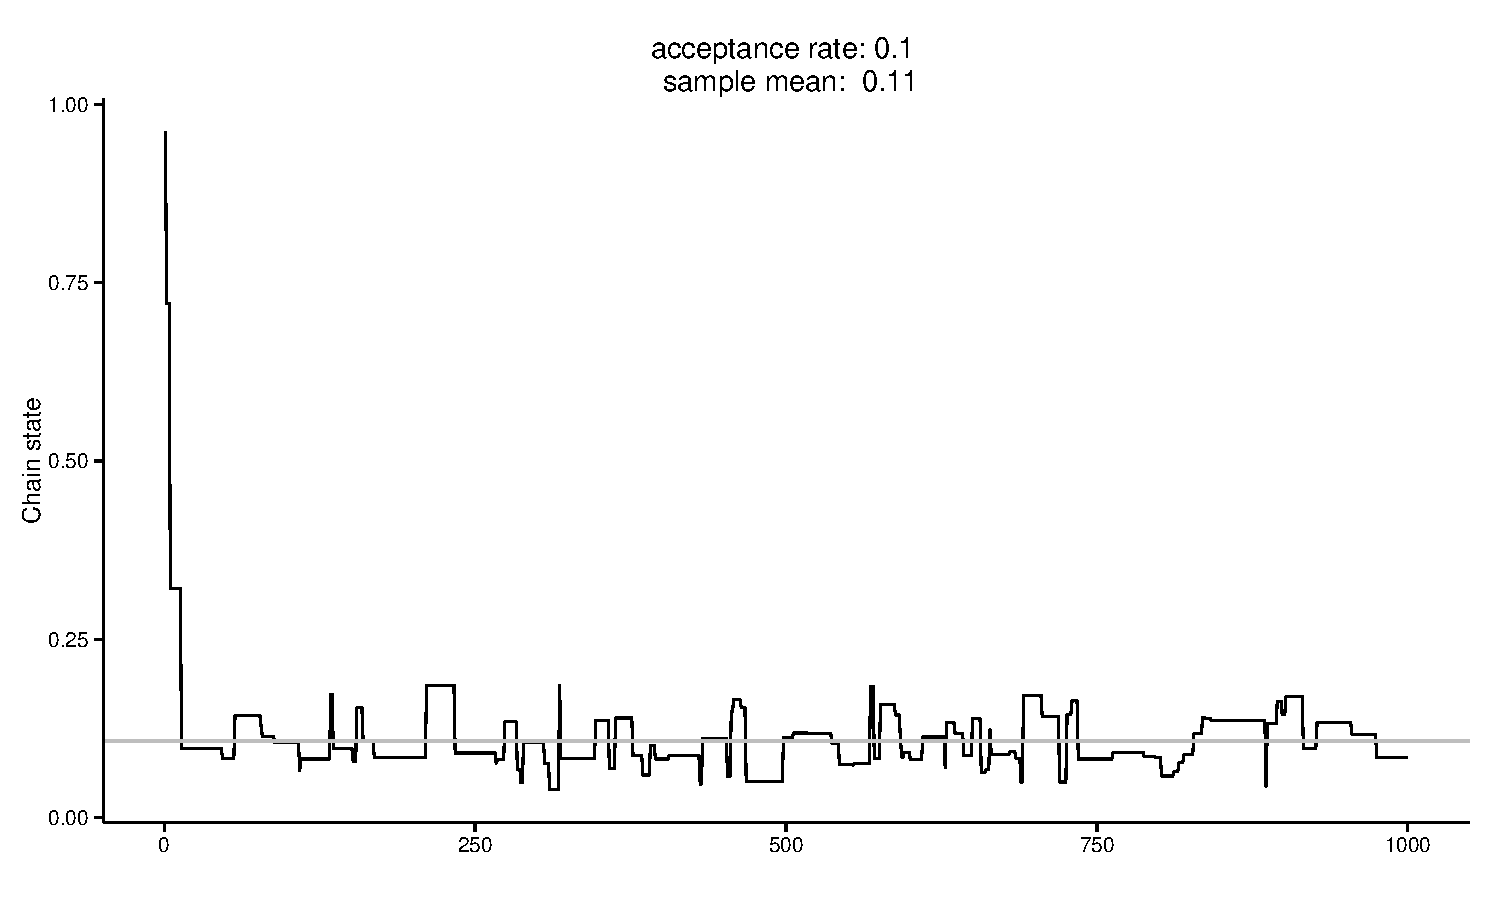
\includegraphics[scale=0.5]{window_size} 
\caption{
{ \footnotesize 
{\bf MCMC output for the same problem as presented in Figure~\ref{fig:metropolis}, with proposal having the window size of $1.0$.}
}% END: footnotesize
}
\label{fig:window_size}
\end{figure}

It is clear from the plot that the proposal is sub-optimal in this case; the large window does not allow for the posterior to be efficiently explored, leading for too many moves to be rejected, which is also apparent when looking at the acceptance rate.
However, this does not mean that the algorithm fails, as it will still reach its stationary distribution \citep{Tierney1994}, although it needs much more samples to do so than the proposal in Figure~\ref{fig:metropolis}. 
For a given sample size a more efficient proposal will produce more samples from the posterior distribution.
The efficiency of the sampler, as measured by the acceptance rate, can thus be viewed as a measure of accuracy of the inferences.

Even for the most basic problems the convergence needs to be formally assessed.
If the iterations of the MCMC algorithm, such as M-H, have not proceeded for long enough, the collected sample may not be representative of the true posterior (target) distribution.
%GB: the term 'sequences' is not a good choice here I think
One recommended approach for assessing convergence of the chain is to compare different simulated calculations starting from different initial values in terms of their within and between chain variance, an approach known as the Gelman and Rubin diagnostics \citep{Cowles1996}. 
If the within chain variation is much less than the between chain variation, the different calculations have clearly not converged.
The weighted average of those variances is then taken as an estimate of the variance of the stationary distribution and is guaranteed to be an unbiased estimator if the starting values come from the stationary distribution.

Trace plots such as the ones in Figures~\ref{fig:metropolis} and~\ref{fig:window_size} are a useful visual aid for assessing the mixing of a single chain.
Density estimates, like the histogram in the bottom panel of Figure~\ref{fig:metropolis} can also help in spotting the most apparent mixing problems that the particular chain might have.
Convergence assessment procedures can only reliably diagnose situations in which the particular chain has failed to converge in the given simulation time, yet they do not guarantee the converse; i.e. that the chain which seems like a convergent one has in fact explored the whole target distribution.

There have been many propositions for improving the convergence of the chain to the equilibrium distribution, see for example \cite{Liu1994, Gelfand1995, Vines1996}.
Even if the MCMC simulations have reached convergence, early collected iterations are still influenced by the starting value.
To reduce the impact of those, the general practice is to discard the first $10\%$ of the collected samples, often referred to as the \textit{burn-in}.

Another problem that frequently arises is inherited from the iterative nature of the algorithm, i.e. the within sequence correlations.
Although not a problem for convergence, as after reaching the target distribution the sampled values are guaranteed to be \textit{iid}, it poses an efficiency problem.
If the collected sequences are used directly to estimate the posterior distribution of the unknown parameter the estimates are generally less efficient, because of that auto correlation.
The Effective Sample Size (ESS) is a frequently used measure of the information that the collected sample size contains.
One of the techniques for reducing auto correlation is called \textit{thinning}, which skips every $k$-th iteration from the sampled sequence. 

\subsection{Bayesian phylogeography\label{sub:phylogeo}}

Phylogeography is a research direction aimed at connecting evolutionary processes, which happen over time, with the processes of spatial dispersal into a joint spatio-temporal dynamic that can be used to track pathogen spread.
<<<<<<< HEAD
Historically, phylogeographic inference in molecular epidemiology ignored the complementary character of these two processes. 
The evolutionary relationship represented by the tree was inferred omitting the geographical information, and then the ancestral locations generated by the process of the spatial diffusion were reconstructed, conditioning on the inferred tree topology.
=======
%GB: I don't like the use of 'reciprocal' here ...
% FB: could also use complementary
Historically, phylogeographic inference in molecular epidemiology ignored the correlated nature of these two processes. 
The evolutionary relationships represented by the tree were inferred were first estimated from the sequence data, and then the ancestral locations generated by the process of the spatial diffusion were reconstructed from the spatial data, conditioning on the inferred tree topology.
>>>>>>> e62f2b18afbdfbcd00243cf6a0a9d0cdbb5e31d0
\citet{Lemey2009} first considered the Bayesian reconstruction that allows for joint inference of both a time-measured evolutionary history and the parameters of the spatial and temporal process that shapes the spread and evolution of 
% e.g. 
rapidly evolving viruses.
This approach does not require fixing the tree topology, the branch lengths nor the Markov model parameters, and allows for integration over all possible values, requiring only for a specification of a prior distributions for the parameters that we aim to infer.

\myedit{svonec}{
Central to the Bayesian phylogeographic framework is the hypothesis that sequence evolution is occurring simultaneously with the process of geographical dispersal. 
The observed data, residing at the $N$ tips of phylogeny $\mathbf{F}$, is recorded as both character sequence data $\mathbf{X}=(X_{1},...,X_{N})$ and discretized geographic locations (countries, districts, cities) $\mathbf{Y}=(Y_{1},...,Y_{N})$, as depicted in the upper facet of Figure~\ref{fig:discrete_phylo_illust}.
We assume independent stochastic processes are responsible for generating these data, with ancestral states of $\mathbf{X}$ generated as before by a CTMC characterized by rate matrix $\mathbf{Q}$ and the unobserved ancestral locations $(Y_{N+1},...,Y_{2N-2})$ generated by a separate CTMC characterized by rate matrix $\mathbf{\Phi}$ (see Figure~\ref{fig:discrete_phylo_illust}, lower facet).
The entries of this matrix are the transition rates $\phi_{ij}$ between locations $i$ and $j$.
Unlike before, the rate matrix does not necessarily have to be symmetrical, i.e. there exist some $i,j$ such that $\phi_{ij}\neq\phi_{ji}$.
Additionally, a priori one would expect many of the infinitesimal rates to be zero. 
}

%---DISCRETE PHYLOGEOGRAOHY ILLUSTRATION---%
\begin{figure}[h!]
\centering
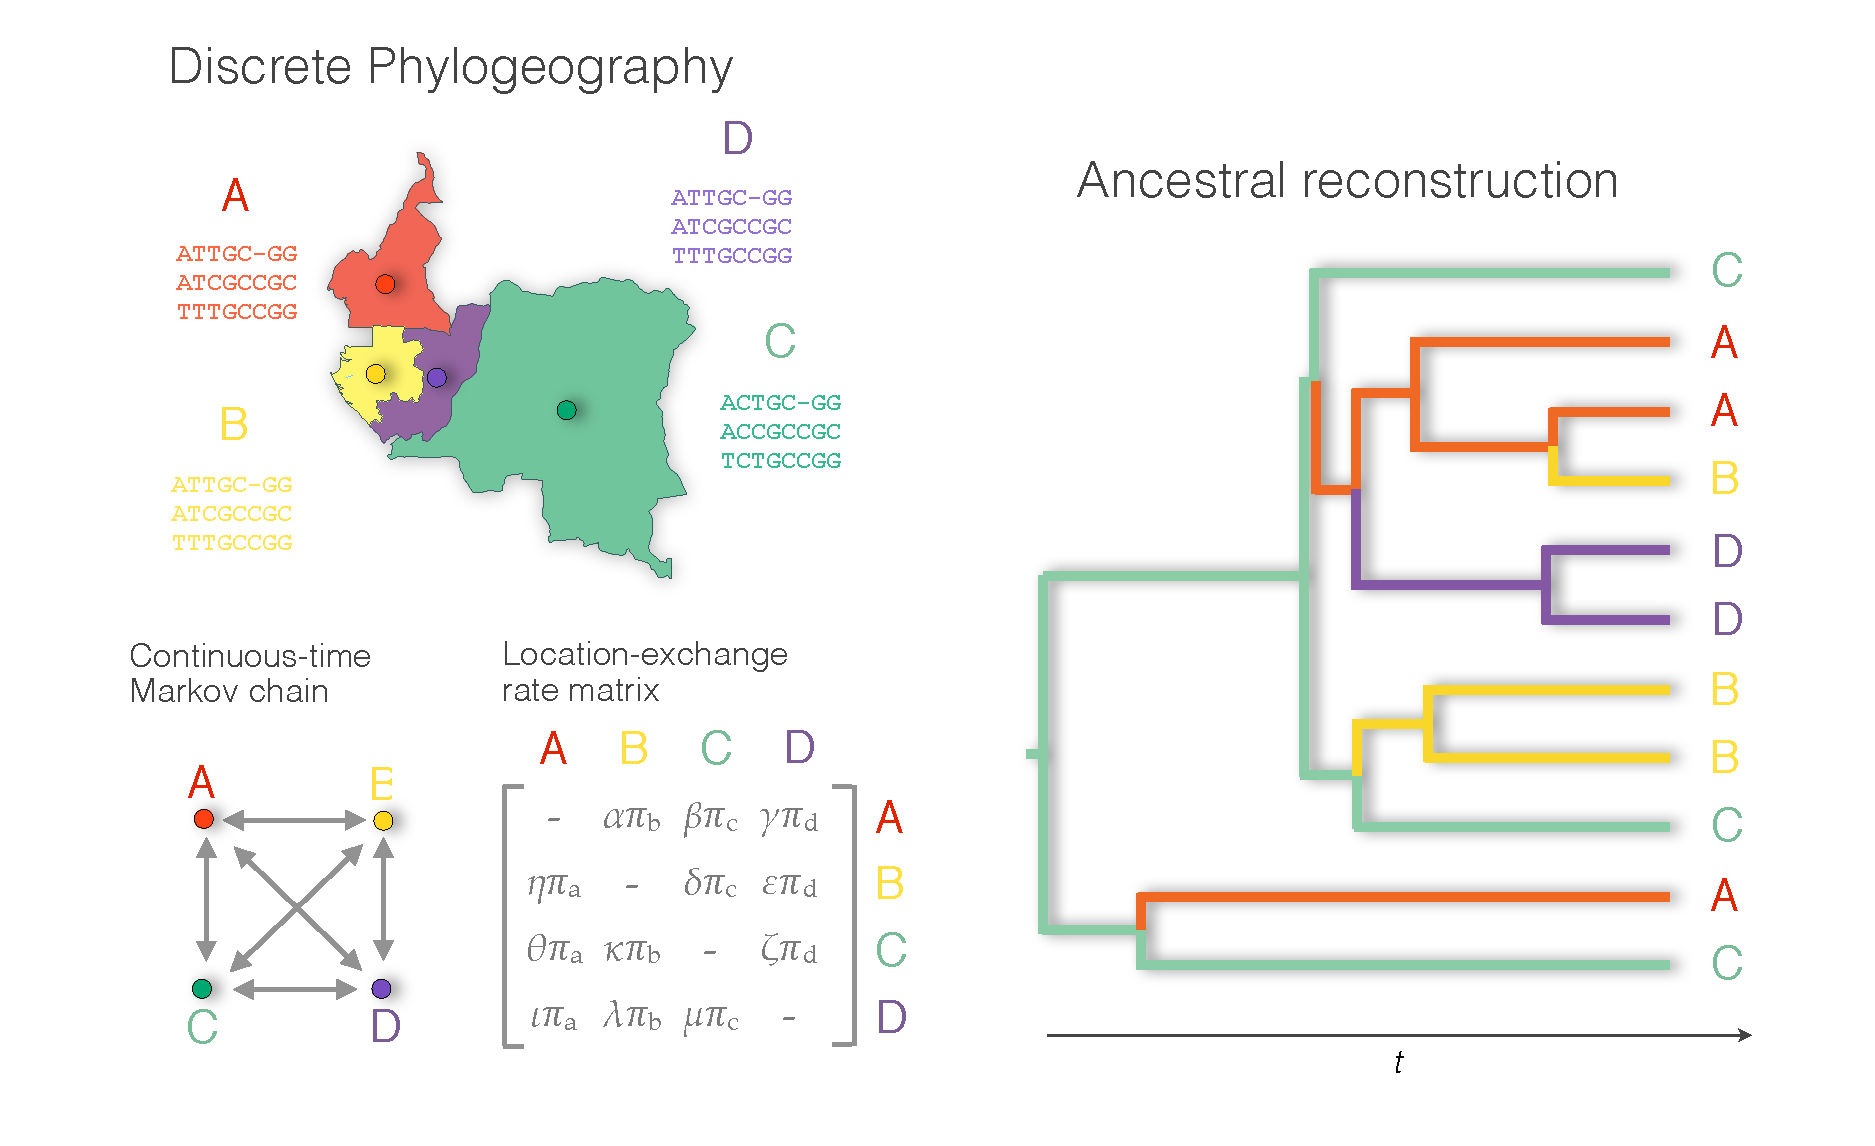
\includegraphics[scale=0.4]{discretePhylogeography} 
\caption{
{ \footnotesize 
{\bf Discrete phylogeographical model for $K=4$ location states.} 
The data consist of both the character sequences and locations at which they were recorded.
The model allows for non-symmetric rates of location exchange in the evolutionary history.
}% END: footnotesize
}
\label{fig:discrete_phylo_illust}
\end{figure}


Unlike the molecular data, which is typically dense, the location data is sparse, with only one observation per taxon and many transitions are likely to remain observed.
For this reason, a Bayesian stochastic search variable selection (BSSVS, see also Subsection~\ref{sub:clocks}) procedure has been proposed in order to allow exchange rates in $\mathbf{\Phi}$ that do not contribute to the phylogeographic diffusion to shrink to zero with a certain probability.

The Bayesian framework described in Subsections~\ref{sub:bayesTheorem} and \ref{sub:mcmc} offers the unique ability to integrate different sources of information about the viruses with their genetic data, without conditioning on either one of them.
We use this ability to infer the tree topology, the ancestral spatial locations and the character substitution process giving rise to the aligned molecular sequence data. 
Since assume independent stochastic processes are responsible for generating these data, we can write down the joint posterior distribution as: 

\begin{align}
P\left(\mathbf{F}, \mathbf{Q}, \mathbf{\Phi}|\mathbf{X},\mathbf{Y}\right) &\propto 
\underbrace{P(\mathbf{X}|\mathbf{Q}, \mathbf{F})}_{\begin{array}{c}
\substack{\text{Sequence} \\ \text{likelihood}}
\end{array}}\cdot\underbrace{P(\mathbf{Y}|\mathbf{\Phi}, \mathbf{F})}_{\begin{array}{c}
\substack{\text{Trait} \\ \text{likelihood}}
\end{array}}\cdot
\underbrace{P(\mathbf{F})}_{\begin{array}{c}
\substack{\text{Topology} \\ \text{prior}}
\end{array}} \nonumber \\
& \cdot \underbrace{P(\mathbf{Q})}_{\begin{array}{c}
\substack{\text{Sequence substitution} \\ \text{prior}}
\end{array}}\cdot\underbrace{P(\mathbf{\Phi})}_{\begin{array}{c}
\substack{\text{Location exchange} \\ \text{prior}}
\end{array}}
\label{eq:posteriorPhylogeography}
\end{align}

The likelihood component for both molecular data $\mathbf{X}$ and location data $\mathbf{Y}$ is calculated using recursive tree pruning, as described in Subsection~\ref{sub:likelihood}.
We approximate the joint posterior as written down in Equation~(\ref{eq:posteriorPhylogeography}) using MCMC methods we discussed in Subsection~\ref{sub:mcmc}, which leads to the reconstruction of the most plausible histories with ancestral location states, as depicted in the left facet of the Figure~\ref{fig:discrete_phylo_illust}.

In order to study phylogeographic processes based on longitude and latitude coordinates of sampled strains, Brownian motion has been proposed as the random walk model in continuous space with conceptually very similar inference procedures \citep{Lemey2010}.


\subsection{Bayesian model selection\label{sub:model_selection}}
% https://radfordneal.wordpress.com/2008/08/17/the-harmonic-mean-of-the-likelihood-worst-monte-carlo-method-ever/

A standard approach to compare models in a Bayesian phylogenetic framework is through the evaluation of Bayes factors (BFs).   
The BF is a ratio of two marginal likelihoods, which given the observed data $\mathbf{X}$ quantify the plausibility of two models, denoted $M_{1}$ and $M_{2}$ and are parametrised in terms of parameters $\theta_{1}$ and $\theta_{2}$ respectively:

% 
\begin{equation}  
\frac{\int P\left(\mathbf{X}|\theta_{1},M_{1}\right)\times P\left(\theta_{1} \mid M_{1}  \right)d_{\theta_{1}}}{\int P\left(\mathbf{X}|\theta_{1},M_{2}\right)\times P\left(\theta_{2} \mid M_{2} \right)d_{\theta_{2}}},
\label{eq:bayes_factor}
\end{equation}  
% 

\noindent
where $P\left(\mathbf{X}|\theta_{i},M_{i}\right)$ is the likelihood function and $P\left(\theta_{i} \mid M_{i} \right)$ is the prior, for $i=1, 2$.
The parameters $\theta_{i},\; i=1, 2$ can be possibly multidimensional, making the integral in Equation~\ref{eq:bayes_factor} non-trivial to estimate.
For a number of years the posterior Harmonic Mean Estimator (HME, \cite{Newton1994}) has been extensively used in Bayesian phylogenetic inference, mainly for the simplicity in its calculation. 
To evaluate the HME one only needs the samples from the posterior distribution which are readily available as output form any MCMC program.

Among others, \cite{Meng1996}, \cite{Lartillot2006} and \cite{Xie2011} warn that despite this computational convenience the HME is a biased estimator of the (log) marginal likelihood, severely overestimating the true value and with potentially infinite variance.
%GB: not typically the correct references for this type of work, so I removed them
This has lead to a substantial amount of work invested in the development of more accurate methods for estimating (log) marginal likelihoods.
To this end, \cite{Lartillot2006} introduced path sampling (PS) into the field of phylogenetics, providing several examples for which the HME was drastically outperformed by PS when estimating the marginal likelihood.
The authors showed that even for simple Gaussian examples, for which the true value of the marginal likelihood can be analytically calculated, the HME was unable to estimate the true underlying value whereas PS proved very reliable for all cases examined. 
Further, for evolutionary models with high dimensions, the HME severely overestimated the (log) marginal likelihood compared to PS, leading to a plausible explanation for many dubious findings concerning model selection over the years.

Recently, \cite{Xie2011} developed stepping-stone sampling (SS) as a computationally more interesting alternative to path sampling (PS).
The authors show that by essentially performing the same calculations as for PS, but using the collected samples in a different way, they are able to compose a more efficient (log) marginal likelihood estimator.
Both PS and SS rely on drawing MCMC samples from a series of distributions, each of which is a power posterior differing only in its power, along the path going from the prior to the unnormalized posterior defined by the model $M$:  

\begin{equation}  
q_{\beta}\left(\theta\right)=P\left(\mathbf{X}\mid\theta,M\right)^{\beta} \times P\left(\theta\mid M\right).
\label{eq:ss_ps}
\end{equation}  

\cite{Baele2012} have performed a comparative study on the performance of HME, the stabilized/smoothed HME (sHME), the AICM (a posterior simulation-based analogue of Akaike?s information criterion through Markov chain Monte Carlo, PS and SS in a phylogenetic framework.
The authors showed that PS and SS consistently outperformed the harmonic mean estimators as well as the AICM when comparing demographic models as well as relaxed clock models.
Although offering tremendous improvements in bias and variance over the HME both PS and SS require considerable computational effort as the (log) marginal likelihood can no longer be estimated from the likelihood trace that is being output from the standard MCMC analysis. 
Further, great care must also be taken to specify proper priors for all parameters in Equation~\ref{eq:ss_ps}, so as to avoid numerical instabilities when the integration approaches the prior \cite{Baele2013b}.  











\cleardoublepage
\chapter{Modeling substitution heterogeneity through time\label{chap:epoch}}

\begin{remark}{Outline}
This chapter is adapted from the following publication: \\
F. Bielejec, P. Lemey, G. Baele, A. Rambaut, and M. A. Suchard. 
Inferring heterogeneous evolutionary processes through time: from sequence substitution to phylogeography. 
Systematic Biology, 2014, 63(4):493 -- 504.
\end{remark}

\section{Abstract}

Molecular phylogenetic and phylogeographic reconstructions generally assume time-homogeneous substitution processes.
Motivated by computational convenience, this assumption sacrifices biological realism and offers little opportunity to uncover the temporal dynamics in evolutionary histories.
%
Here, we propose an evolutionary approach that explicitly relaxes the time-homogeneity assumption by allowing the specification of different infinitesimal substitution rate matrices across different time intervals, called epochs, along the evolutionary history.
%
We focus on an epoch model implementation in a Bayesian inference framework that offers great modeling flexibility in drawing inference about any discrete data type characterized as a continuous-time Markov chain, including phylogeographic traits.
To alleviate the computational burden that the additional temporal heterogeneity imposes, we adopt a massively parallel approach that achieves both fine- and coarse-grain parallelization of the computations across branches that accommodate epoch transitions, making extensive use of graphics processing units.
%\par
Through synthetic examples, we assess model performance in recovering evolutionary parameters from data generated according to different evolutionary scenarios that comprise different numbers of epochs for both nucleotide and codon substitution processes. 
We illustrate the usefulness of our inference framework in two different applications to empirical data sets: the selection dynamics on within-host HIV populations throughout infection and the seasonality of global influenza circulation.
In both cases, our epoch model captures key features of temporal heterogeneity that remained difficult to test using \textit{ad hoc} procedures.

\section{Introduction}

Molecular phylogenetic models typically consider sequence evolution as a continuous-time Markov chain (CTMC) that operates along the branches of a bifurcating tree.
As a description of the character substitution process, CTMCs take their values from a finite set of discrete states called the state space and satisfy the Markov property.
The Markov property ensures that the process is memoryless, implying that the conditional probability distribution of future states only depends upon the present state, and not on the preceding sequence of events.
CTMCs are characterized by matrices of infinitesimal rates that quantify the probabilities of exchanging discrete characters in an infinitely small time interval.

Current CTMC models are not limited to nucleotide or amino acid data, frequently accommodate large state spaces, such as codon substitution models \citep{Goldman1994, Muse1994}, and generalize to many discrete data types including spatial locations (e.g. cities or countries) in phylogeographic inference \citep{Lemey2009} or hosts in analyses of viral cross-species transmission \citep{Faria2013, Mather2013}.
In the latter cases, not only can the state space be large but also the underlying substitution rate matrix may be asymmetric.

Phylogenetic inference often resorts to substitution processes that are stationary, homogeneous and reversible.
Stationarity dictates that the process is at equilibrium, such that the frequency distribution of realized states remains constant over the course of evolution. 
Homogeneity ensures that the process is constant in pattern throughout evolutionary history, thereby treating evolution as a lineage- or time-independent process.
This implies that nonstationarity induces nonhomogeneity, as the process of evolution depends upon the equilibrium frequencies.
However, a process can be stationary but not homogeneous, e.g. through the specification of different instantaneous rate parameters for different partitions of the underlying tree topology.
Finally, reversibility is a frequently applied restriction to the rate matrix describing molecular evolutionary processes that leads to a reduced number of free parameters.
Collectively, these restrictive assumptions make strong abstraction of the underlying substitution process to ease mathematical and computational tractability.

In recent decades, substantial work has aimed at relaxing the standard assumptions in CTMC processes, in order to uncover more complex evolutionary processes and assess their impact on phylogenetic reconstruction. 
To accommodate nonstationarity, \citet{Yang1995}, \citet{Galtier1998} and \citet{Galtier1999}, for example, have proposed models that allow branch-specific nucleotide compositions.
Although this includes general treatments involving separate composition parameters for each tree branch, large trees will inevitably lead to over-parameterized models.
To address this problem, \citet{Foster2004} has developed an approach that maps a restricted, but fixed number of nucleotide composition vectors with estimable frequencies to the tree. 
%TODO
% \myedit{svfifteen}{
Set in a Bayesian framework, this approach also integrates over the tree topology and finds improved posterior support estimates for topologies in examples with compositional heterogeneity, allowing for different CTMC stationary frequencies in the evolutionary history, 
as opposed to inference under a stationary model that would suffer from attraction artifacts due to similar compositional biases. 
% }
Further developments have uncoupled compositional shifts from particular nodes in the tree while estimating the total number of events of compositional drift distributed across the tree using a compound Poisson process \citep{Blanquart2006}. 
\cite{Blanquart2008} have also combined such approaches for amino acid evolution with models that take into account site-specific substitution patterns induced by protein structure and function.

Models also exist to tackle nonhomogeneity in the instantaneous rates of character exchange rather than perturbing stationarity.
Homogeneous substitution rates can be relaxed both among sites \citep{Huelsenbeck1999} and among branches (e.g., \citet{Foster12082009}), and in both cases this captures additional complexity in the substitution process in different data sets. 
In codon substitution models, among branch variation in the non-synonymous to synonymous substitution rate ratio ($d_N/d_S = \omega$) allows testing and quantifying varying selective pressure among lineages \citep{Yang1998}.

\par  % MAS: new paragraph to highlight change

Tree-based modeling of heterogeneity in the pattern of evolution typically finds its use when applied to widely divergent taxa representing relatively rich speciation histories and possibly involving lineage-specific adaptation.

However, a change in the evolutionary process may also apply to an entire population at a particular point in time, in which case the evolutionary shift simultaneously cuts across all lineages at that time point in the underlying genealogy, creating discretized time intervals that we refer to as epochs.
\citet{Goode2008} first consider such a scenario; they develop an extension of a codon substitution model with discrete site classes that allows for a time-specific change in $\omega$ and in the transition/transversion rate ratio ($\kappa$), and estimate probabilities that sites belong to a particular class.
Specifying such change-points requires trees measured in time and so \citet{Goode2008} adopt a strict molecular clock model on a fixed tree topology in order to apply the model to HIV envelope sequences sampled from a single patient over a period of three years.  
Because the rapidly evolving virus population accumulates significant substitutions over such a short time-scale, one can estimate the rate of evolution by incorporating the sampling dates of the sequences (the `dated tip' model, \citet{Rambaut2000}).
The authors demonstrate that many sites classified as neutral or under positive selection before therapy appear to be under strong negative selection upon treatment initiation.

Although we do not pursue codon substitution models with different site classes in this work, we build upon the approach of \citet{Goode2008} in several important ways.
By implementing a similar model of time-specific evolutionary changes in the Bayesian Evolutionary Analysis by Sampling Trees (BEAST) software package \citep{Drummond2012}, 
we connect the epoch models to different relaxed clock models that often provide a more realistic description of the tempo of evolution \citep{Drummond2006, Drummond2010}.
More importantly, we generalize the epoch model to any finite discrete data type and any number of transition times.
The former is critical to accommodate discrete phylogeographic inference \citep{Lemey2009}, for which \citet{Bahl2011} recently demonstrate the need to incorporate time-specific migration rates.
Our Bayesian approach also does not condition on a fixed tree topology but averages over all plausible evolutionary histories.  
This integration naturally accounts for uncertainty in the tree and in how the epoch transition times translate to varying branch-specific change points.
Jointly estimating the epoch-associated rate matrices and the unknown evolutionary history also ensures that we can fully exploit our Bayesian phylogeographic (or discrete trait evolutionary) inference, which explicitly connects sequence evolution to the trait diffusion process \citep{Lemey2009}.
Finally, our implementation also allows us to make use of recent marginal likelihood estimators to assess model fit for different epoch parameterizations \citep{Baele2012}.

Statistical phylogenetic inference can be computationally demanding, especially when confronted with the current flood of sequence data.
Recently, however, new algorithms have been developed to exploit massive parallelization on graphics processing units (GPUs), offering dramatic speed increases for statistical inference under complex evolutionary models \citep{Suchard2009,Baele2013}.
By partitioning the time component into discrete intervals, the epoch model further adds to the computational burden, but it also represents an opportunity to exploit massive parallel computation \citep{Suchard2009,Suchard2010}. 
To apply the epoch substitution heterogeneity in conjunction with large-state space models to large data sets, we implement our model as part of the Broad-platform Evolutionary Analysis General Likelihood Evaluator (BEAGLE) library for evaluating the likelihood of sequence evolution on trees \citep{Ayres2012}, taking the effort to accommodate multiple scales of parallelization to keep computation time manageable. 

Following \citet{Goode2008}, we mainly focus on rapidly evolving populations for which significant divergence accumulates between sequences sampled at different time points, both from the simulation perspective and for the real data sets.
Using a simulation study we demonstrate that our model can be fit 
to complex data sets and consistently captures time-specific evolutionary parameters, but is not restricted to time-stamped data.
We further demonstrate the use of our model by examining two real-life examples. 
The first application tests and quantifies changes in $d_N/d_S$ associated with HIV disease progression in several different patients. 
This analysis aims at testing different hypotheses explaining why viral divergence stabilizes close to disease onset in HIV infection \citep{Shankarappa1999}. 
The second application employs epoch modeling to accommodate seasonality in the inference of global influenza dispersal dynamics. 

%---METHODS---%
\section{Methods}

Continuous-time Markov chain substitution models provide the cornerstone of computational phylogenetics.  Given a discrete trait obtaining $K$ distinct states, a $K \times K$ infinitesimal rate matrix $\mathbf{Q}$ characterizes its CTMC. Matrix $\mathbf{Q}$ contains instantaneous transition rates $q_{ij} \ge 0$ for $i \neq j$ and
satisfies $\mathbf{Q} \mathbf{1} = \mathbf{0}$, where $\mathbf{1}$ and $\mathbf{0}$ are $K \times 1$ column vectors.

From the rate matrix $\mathbf{Q}$, a stochastic matrix $\mathbf{P}$ is computed over time $t \geq 0$ via matrix exponentiation $\mathbf{P}(t)=
\exp(t\mathbf{Q})
=\underset{j=0}{\overset{\infty}{\sum}}
(t\mathbf{Q})^{j} / j!$. For an overview of methods to numerically approximate a matrix exponential, we refer to \citet{Moler1978}.
%
Drawing realizations with probabilities defined by $\mathbf{P}$ gives rise to a stochastic process $\left\{ X(t):\; t\geq0\right\}$ satisfying the Markov property, such that for every $n\geq 0$, given the time points $0\leq t_{0}\leq t_{1}<\ldots<t_{n}\leq t_{n+1}$ and discrete states $i_{0},i_{1}, \ldots, i_{n},i_{n+1}$ it holds that %\newline
%
$P\left\{ X(t_{n+1})=i_{n+1}\mid X(t_{n})=i_{n},\ldots, X(t_{0})=i_{0}\right\} =P\left\{ X(t_{n+1})=i_{n+1}\mid X(t_{n})=i_{n}\right\} $. 
%
In general, one refers to the elements of $\mathbf{P}$ as finite-time transition probabilities between the $K$ discrete state-space elements. Let us denote a transition probability between two states $i$ and $j$ over time $u$ to $t+u$ by

\begin{equation}
p_{ij}\left(u,t+u\right)=P\left\{ X(t+u)=j\mid X(u)=i\right\} .
\end{equation}

In the phylogenetic setting, researchers often further constrain these processes 
to be time-homogeneous and time-reversible. Time-homogeneity mandates that  transition probabilities depend only on the difference $t$ between times $u$ and $t + u$,

\begin{equation}
p_{ij}\left(u,t+u\right)= p_{ij}\left(0,t\right) \equiv p_{ij}\left(t\right) .
\end{equation}

Time-reversible CTMCs satisfy detailed balance, such that $\pi_{i}p_{ij}(t)=\pi_{j}p_{ji}(t)$ for all $i$, $j$ and $t$, where $\pi_j = p_{ij}(\infty)$ for all $j$ return the stationary distribution of the CTMC and are independent of starting state $i$.  
Finally, common practice in phylogenetics reparametrizes the elements of $\mathbf{Q}$ into relative rates through the constraint $\sum_i \pi_i q_{ii} = -1$ and then, for studies involving phylogenies set in calendar time, multiples $\mathbf{Q}$ by a rate scalar $r$ to form the argument to $\mathbf{P}(t)$. 
In this case, we define

\begin{equation}
p_{ij}(u,t+u,r) 
=
\left\{
\exp(
r  t  \mathbf{Q})
\right\}_{ij}
,
\label{eq:makeprobs}
\end{equation}

where $\{ \cdot \}_{ij}$ extracts the $ij$-th element.

\newcommand{\tmax}{t_{\mbox{\tiny max}}}

\citet{Felsenstein1981} provides an efficient algorithm for computing the likelihood of a phylogenetic tree $\mathbf{F}$ given discrete traits and the finite-time transition probabilities along each branch of $\mathbf{F}$.
Label the nodes $x_{1},\ldots,x_{2N-1}$ in an $N$-tipped $\mathbf{F}$ set in calendar time%
.
Now, consider a trio of nodes $u$, $v$ and $w$ where node $u$ lies at time $t_{u}$ in the past and is parent to both nodes $v$ and $w$, at times $t_v$ and $t_w$, respectively, in $\mathbf{F}$.
Then we imagine that an unobserved discrete trait $i$ evolves independently into $j$ at node $v$ over the time interval $\left[t_{u},t_{v}\right]$ with rate scalar $r_{v}$ and into $k$ at node $w$ over $\left[t_{u}, t_{w}\right]$ with rate scalar $r_{w}$.

Visiting all the nodes in post-order fashion, we can integrate out these unobserved traits, calculating successive contributions to the partial likelihood for each node via

\begin{equation}
L_{x_{u}}(i)=
\left[\underset{j}{\sum}p_{ij}(t_{u},t_{v},r_{v})L_{x_{v}}(j)\right]
\times
\left[\underset{k}{\sum}p_{ik}(t_{u},t_{w},r_{w})L_{x_{w}}(k)\right].
\label{eq:partial_likelihood}
\end{equation}

For tip nodes in $\mathbf{F}$, we assign $L_{x_{u}}(i)$ to either $0$ or $1$ depending on whether trait $i$ is (partially) observed or not.  Finally, the full likelihood of $\mathbf{F}$ becomes $\sum_{i} L_{x_{2n-1}}(i) \pi_{i}$, where $x_{2N-1}$ is the root node.  For multiple traits or sequences of length $L$ and for among-site rate mixtures with $C$ categories, one assumes conditional independence across sites and rate categories and simply aggregates site-category contributions.  The serial computational order of this recursion is ${\cal O}( K^2 \times N \times C \times L)$.  

Central to the recursive tree-pruning in Equation (\ref{eq:partial_likelihood}) is specification of the branch-specific transition probabilities
$\mathbf{P}(t_u, t_v, r_v) = \left\{
p_{ij}(t_u,t_v,r_v)
\right\}$ for all $i,j$.  These are commonly homogeneous and conveniently collapse into
functions of just the branch length $t_u - t_v$ instead of the more elaborate starting and ending time.
A strict molecular clock assumption specifies that all $r_u$ are equal, but this is not a necessary restriction of our model because we can allow for the introduction of lineage-specific rate variation in addition to the time-inhomogeneity in substitution processes that we tackle next. 

%---RELAXING TIME HOMOGENEITY---%
\subsection{Relaxing time-homogeneity}

The epoch model finds its use in situations where the usual time-homogeneity assumption is violated in specifying $\mathbf{P}(t_u, t_v, r_v)$. 
To model inhomogeneity in process through time, we assume that there exist $S$ unique substitution processes characterized through rate matrices $\mathbf{Q}_s$ for $s = 1,\ldots,S$, and that, at any given point in time, one of these processes is active across all of the extant lineages in $\mathbf{F}$. 
We then model how the active process changes over time via a change-point process with $M + 1$ ordered boundaries at times 
$-\infty = T_0 < T_1 < \cdots < T_{M-1} < T_{M} = \tmax$, where $\tmax$ is the time of the most recently observed tip in $\mathbf{F}$, 
and $M$ indicator functions $\phi_m\ \in\ \{1,\ldots,S\}$ that identify which $\mathbf{Q}_{\phi_m}$ is active during the time epoch 
% $\left(T_{m-1}, T_{m}\right)$.
$\left[T_{m-1}, T_{m}\right]$.
For the examples in this paper, we assume that $S$, $M$ and $(T_m, \phi_m)$ for all $m$ are fixed through marked biological constraints.  

To compute $\mathbf{P}(t_u, t_v, r_v)$ for each branch in $\mathbf{F}$ under this change-point process, we return to the Markov property of CTMCs that says one only needs to keep track of the immediate past in determining transition probabilities for the future.  
This greatly simplifies and regularizes computation, allowing for its parallelization.  Assume $t_u$ lies in epoch $m^{\prime}$ and $t_v$ lies in epoch $m^{\prime\prime}$.  If $m^{\prime} = m^{\prime\prime}$, then no new work is necessary.  We compute these transition probabilities directly via Equation (\ref{eq:makeprobs}) from an eigen-decomposition of $\mathbf{Q}_{m^{\prime}}$; \citet{Suchard2009} describe parallelization of this work across branches and rate categories.
On the other hand, if $m^{\prime} \neq m^{\prime\prime}$,
the branch traverses $m^{\prime\prime} - m^{\prime}$ epoch boundaries at which times $\mathbf{Q}$ changes. To handle these discontinuities, we imagine a data augmentation procedure to break the inhomogeneous process into a conditionally independent series of homogeneous processes and then integrate out the augmented data.

%---CONVOLUTION ILLUSTRATION---%
\begin{figure}[h!]
\centering
\begingroup
\everymath{\displaystyle}
{\Large
\begin{displaymath} % 
    \xymatrix{ 
    \bullet^{t_u} \ar@{.>}[rr]_{\mathbf{P}_{1}(t_{u},T_{1},r_v)} && \bullet^{T_1} \ar@{.>}[rr]_{\mathbf{P}_{2}(T_{1},t_{v},r_v)} && \bullet^{t_v} \\
    \bullet^{t_u} \ar@{.>}[rrrr]_{\mathbf{P}(t_{u},t_{v},r_v)} & & & & \bullet^{t_v}
    } % 
\end{displaymath}
}
\endgroup
\caption{
{ \footnotesize 
{\bf Collapsing branches.} Transition probability matrix $\mathbf{P}(t_u,t_v,r_v)$ governs the inhomogeneous substitution process along a branch from time $t_u$ to $t_v$ and is the matrix-product of transition matrices $\mathbf{P}_{1}(t_u,T_1,r_v)$ and $\mathbf{P}_{2}(T_1,t_v,r_v)$, where $T_1$ is the epoch change-point time between homogeneous processes 1 and 2.  We assume rate scalar $r_v$ remains constant along the entire branch.
} % END: footnotesize
}
\label{fig:collapsing}
\end{figure}

% \myedit{svseventeen}{
Figure~\ref{fig:collapsing} illustrates this action for a branch that spans a single boundary at known time $T_1$ with $\mathbf{Q}_1$ governing the process before the boundary and $\mathbf{Q}_2$ after the boundary. Letting $X(T_1) = k$ represent the augmented state of the stochastic process at the boundary, we compute:
% }

\begin{align}
p_{ij}(t_u, t_v, r_v)
= \sum_{k} 
\left\{
\exp[ r_v ( T_1 - t_u ) \mathbf{Q}_1]
\right\}_{ik} & \nonumber \\
\times 
\left\{
\exp[ r_v ( t_v - T_1 ) \mathbf{Q}_2]
\right\}_{kj} & , 
\end{align}

\noindent
for all $i,j$, or equivalently in compact matrix form

\begin{align}
\mathbf{P}(t_u, t_v, r_v)
&= 
\exp[ r_v ( T_1 - t_u ) \mathbf{Q}_1]
\times
\exp[ r_v ( t_v - T_1 ) \mathbf{Q}_2] \nonumber \\
&= \mathbf{P}_{1}(t_u, T_1, r_v) \times \mathbf{P}_{2}(T_1, t_v, r_v) ,
\label{matrixProduct}
\end{align}
where 
$\mathbf{P}_{1}(t_u, T_1, r_v)$ and $\mathbf{P}_{2}(T_1, t_v, r_v)$ are shorthand notation used in the figure and again in the next section where it is clear we are considering substitution models for neighboring epochs.

\par

We colloquially refer to the action of Equation (\ref{matrixProduct}) as a transition probability matrix convolution to remind the reader that we are integrating out an unobserved state in the middle, but in a strict sense, this action is simply matrix multiplication and exemplifies a Chapman-Kolmogorov equation \citep[see, e.g.,][]{Feller1}, %(e.g. \citet{Feller1}), 
% describing short time evolution of a stochastic process that realizes discrete outcomes. 
stating that every stochastic process emitting discrete outcomes as a function of time can be marginalized over one of its variables.

For general $m^{\prime} \neq m^{\prime\prime}$, we arrive at
\begin{align}
\mathbf{P}(t_u, t_v, r_v)
= 
& \exp[ r_v ( T_{m^{\prime}} - t_u ) \mathbf{Q}_{\phi_{m^{\prime}}}] \ \times %\nonumber \\
%& 
\prod_{
\nu = m^{\prime} + 1
}^{
m^{\prime\prime} - 1
}
\exp[ r_v ( T_{\nu} - t_{\nu - 1} ) \mathbf{Q}_{\phi_{\nu}}]
 \nonumber \\
&
\quad \times
\exp[ r_v ( t_v - T_{m^{\prime\prime}} ) \mathbf{Q}_{\phi_{m^{\prime\prime}}}] 
.
\label{eq:convolution}
\end{align}

Each matrix convolution in Equation (\ref{eq:convolution}) is ${\cal O}(K^3)$, potentially commanding a high computational burden compared to the likelihood recursion when $K$ is large and many branches in $\mathbf{F}$ transect multiple boundaries.  
Fortunately, these operations are very regular and both fine- and coarse-grain parallelization offers a solution to the computational burden.

\subsection{Fine-grain parallel implementation\label{sub:fine_grain}}

In this subsection, we describe the fine-grain parallel implementation of the epoch model in the BEAGLE library \citep{Ayres2012}.
Pursuing the single instruction, multiple data (SIMD) programming paradigm, GPUs use a thread management system that executes many, possibly millions of lightweight threads at a relatively modest speed, rather than a limited number of threads very rapidly on multiple-core CPUs.
Concurrent threads are grouped into blocks and blocks are organized as a two-dimensional grid, with their sizes specified upon invocation of the function executed on the device, referred to as a kernel. 
On the current NVIDIA GPU architecture, a grid can consist of thousands of thread blocks, each containing hundreds of threads, thus resulting in a fine-grain data parallelism.
Threads on the grid share a common memory address space referred to as the global memory, while threads belonging to the same block share a very fast user-managed cache, known as shared memory.  
Global memory access is the slowest, but it also comprises the largest memory region, measured in GByte orders of magnitude on current architectures, whereas shared memory size is much more limited and measured in KBytes.

The BEAGLE API allows allocating memory for the subsequent tree-pruning operations, as well as specifying key features of the character data and substitution model.  
BEAGLE efficiently performs numerical calculation of transition probability matrices from eigen decompositions of the rate matrices $\mathbf{Q}_{s}$ for arbitrary rate scalar $r$ and edge length $t$.

This approach is highly efficient as the repeated evaluations of $\exp\left(rt\mathbf{Q}_s\right)$ for different $r$ and $t$ reuse the same decomposition of the rate matrix.
Calculating the diagonal matrix of the resulting decomposition of $\exp\left(rt\mathbf{Q}_s\right)$ only involves scaling and exponentiating the eigenvalues of $\mathbf{Q}_s$, effectively reducing the time-consuming calculations to dense matrix-vector-matrix multiplication.
BEAGLE achieves both 
fine-grain parallelism here via massive SIMD reduction of the matrix-vector-matrix multiplication and
coarse-grain parallelism by computing transition matrices across branches in parallel.  

\newcommand{\blockSize}{\ensuremath{B}}

Discretizing the time component introduces additional layers of complexity to the likelihood computations. 
Multiple rate matrices determine the substitution process along branches that traverse different epochs, requiring piecewise matrix convolution operations to arrive at the common process operating on such branches.  
First, we pursue fine-grain parallelism for dense matrix-matrix multiplication by breaking up the problem into smaller sub-problems that fit into the limited amount of shared memory. 
This involves multiplication within a block matrix in which, following the notation from Figure~\ref{fig:collapsing}, each one of the $K \times K$ matrices $\mathbf{P}_{1}(t_u, T_1, r_v)$, $\mathbf{P}_{2}(T_1, t_v, r_v)$ and the product matrix $\mathbf{P}(t_u, t_v, r_v)$ are partitioned into $\blockSize \times \blockSize$ sub-matrices. 
We choose the sub-matrix dimensions such that $\blockSize$ is a multiple of $K$ when possible to avoid thread-divergence. 
Every entry in $\mathbf{P}(t_u, t_v, r_v)$ is therefore computed as:

\begin{equation}
\left\{ \mathbf{P}(t_{u},t_{v},r_{v})\right\} _{ij}=\underset{0\leq k\leq
K / \blockSize
}
{\sum}\left\{ \mathbf{P}_{1}(t_{u},T_1,r_{v})\right\} _{ik}\times\left\{ \mathbf{P}_{2}(T_1,t_{v},r_{v})\right\} _{kj} .
\end{equation}

This strategy executes all sub-problems in parallel%
, with each thread computing a dot product of row-vector  
$\left\{ \mathbf{P}_{1}(t_{u},T_1,r_{v})\right\} _{i\cdot}$  
and column vector 
$\left\{ \mathbf{P}_{2}(T_1,t_{v},r_{v})\right\} _{\cdot j}$ 
stored and reused across threads in shared memory to produce thread-specific element 
$\left\{ \mathbf{P}(t_{u},t_{v},r_{v})\right\} _{ij}$ 
that transfers to global memory only once. 

\subsection{Coarse-grain parallel implementation}

We leverage coarse-grain parallelism by collecting sets of independent matrix update and convolution operations across branches through a post-order tree traversal and executing the same operations simultaneously on the GPU.
To this end, our BEAST/BEAGLE implementation includes a front-end routine that keeps track of branches spanning multiple epochs, the time they spend in each epoch and the order of convolutions for asynchronous dispatch.
This routine interfaces with BEAGLE via its application programming interface (API), making calls to the original parallel BEAGLE kernel \emph{UpdateTransitionMatrices} to calculate finite-time transition matrices and the new \emph{ConvolveTransitionMatrices} kernel to multiply two transition matrices into a third product matrix.
%
Although BEAGLE focuses on evaluating likelihoods of character evolution on phylogenies, BEAGLE has no notion of a tree structure and operates directly on the data, i.e.~indexed, column-major flattened out matrices residing within BEAGLE-managed memory, called buffers.
%
\par
For each branch, the post-order traversal computes a set of weights that measure the times that each of the substitution processes is active on that branch, summing to the total branch length. 
If a branch's entire weight is within a single interval, no extra work is needed and the finite time transition probabilities are calculated from the eigen decomposition of the single rate matrix active in that interval.
If the branch spans over multiple epochs, partial transition matrices are formed from the weights and eigen decompositions specific to the corresponding intervals.
For those weights that are non-zero in the same time interval, we first push their corresponding buffers to an update queue.  After the update queue grows full, it gets dispatched for parallel execution, and then we begin to place convolve operations in an convolve queue. 

Our implementation keeps track of two work queues, grouping update and convolve operations in the correct order for later execution on the device. 
A single work item in the queue responsible for updating transition matrices will include one buffer that needs to be populated by finite-time transition probabilities, whereas a work item in the queue that convolves transition matrices will have two input buffers and one output buffer for storing the result of the matrix-matrix multiplication. 
Both work queues utilize a first in, first out (FIFO) abstraction 
to guarantee that the input buffers in the convolution are non-empty, having  been populated by the update operation. 
The buffers for which tasks have been completed are then returned to the pool of extra buffers for further use.

We coordinate the routine workload via asynchronous work queues because of the limited amount of resources available on the device. A single instance of BEAGLE is invoked with a fixed number of allocated buffers, and at present, it is not dynamically increased.
In the Bayesian inference framework utilized by BEAST, the number of convolution operations becomes random and may well exceed the size set for our buffers.
The amount of required buffers further increases by the need to perform convolution operations on a single branch sequentially  
(see Equation \ref{eq:convolution}) and partial results need to be stored before their dependencies are processed and the work can continue. 
When creating a BEAGLE instance, we allocate a number of extra buffers in addition to the buffers that hold transition matrices for each branch. 
Those buffers are then used to store partial transition matrices and results of matrix-matrix multiplications operations. 
Our routine performs operations in batches of equal or smaller size compared to the number of allocated buffers, by pushing those queues to the GPU for parallel execution once the routine has no more buffers available or all work items are queued. Figure~\ref{fig:UpdateConvolveExample} presents an example of update-convolve routine using an asynchronous queue. 

A tutorial which explains how to set up an `epoch model' for analysis in BEAST can be found in Appendix~\ref{app:spread_tuto}.

%---UPDATE-CONVOLVE INFOGRAPHIC---%
\begin{figure}[h!]
\centering
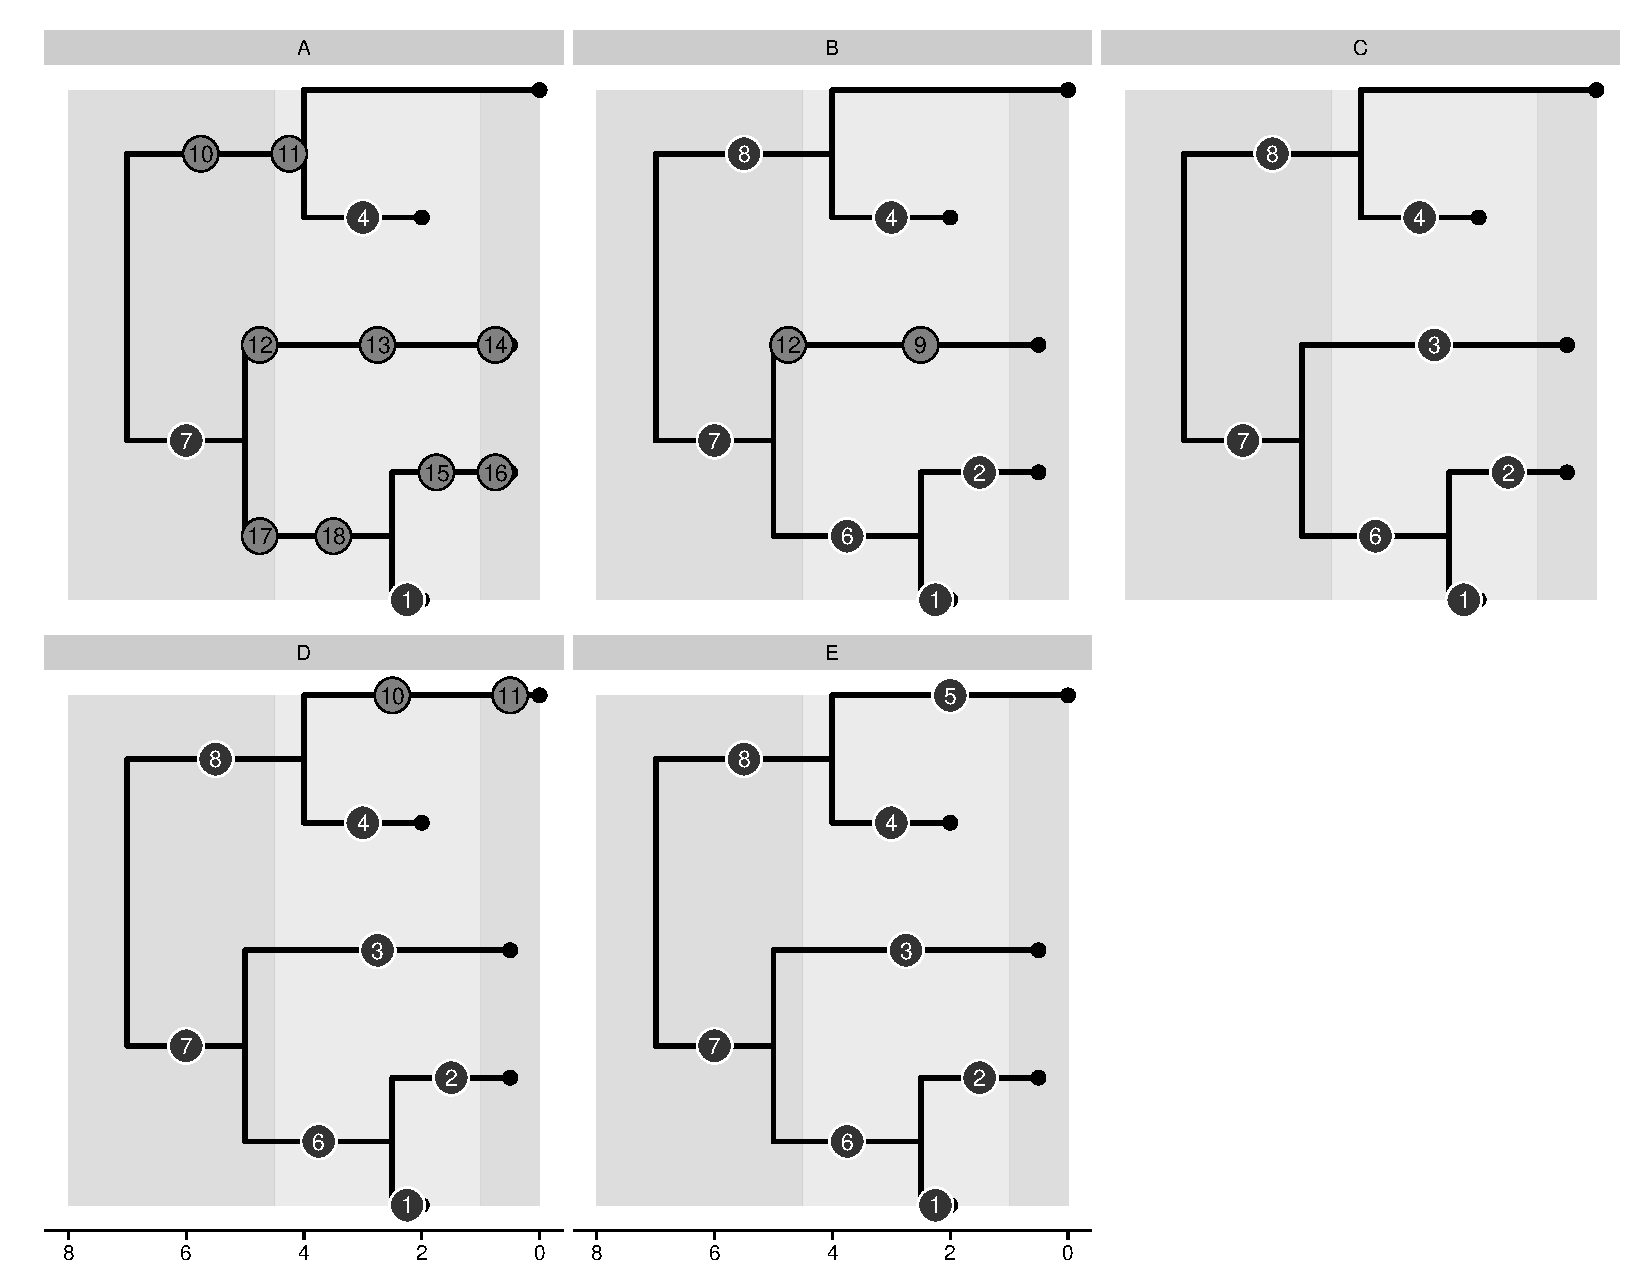
\includegraphics[scale=0.35]{infographic} 
\caption{
{ \footnotesize 
{\bf A small-scale example of the update convolve routine for a 5-taxon tree.} 
In this example, transition times are set at $t_{1} = 1.0$ and $t_{2} = 4.5$, creating three respective epochs indicated by alternating background.
Black dots represent transition probability buffers for particular branches, grey dots denote extra buffers allocated for partial transition matrices.
We allocate 10 extra buffers.  
Consecutive panels illustrate the order of update and convolve steps in the routine.
Update step in A adds buffers to the update work queue. 
In B and C, the routine starts adding buffers to the convolve queue in a stepwise fashion, dictated by the tree traversal, freeing extra buffers whenever the queue is dispatched for execution. 
In D, the routine uses freed buffers for a new update step.
In E, the parallel convolve queue is used to compute the final transition matrix stored in buffer 5, concluding the work.
}% END: footnotesize
}
\label{fig:UpdateConvolveExample}
\end{figure}

%%%%%%%%%%%%%%%
%---RESULTS---%
%%%%%%%%%%%%%%%
\section{Results}

\subsection{Performance assessment using simulation}

To evaluate the performance of the epoch model, we conduct a simulation study, in which replicate data are generated along an evolutionary history inferred from a real data set with samples collected at different points in time.
Specifically, we use a maximum clade credibility (MCC) tree summarizing a Bayesian phylogenetic inference of human influenza A hemagglutinin gene sequences sampled through different epidemic seasons \citep{Drummond2010}. 


%---TOPOLOGY FOR SIMULATIONS---%
\begin{figure}[h!]
\centering
% \color{fgcolor}
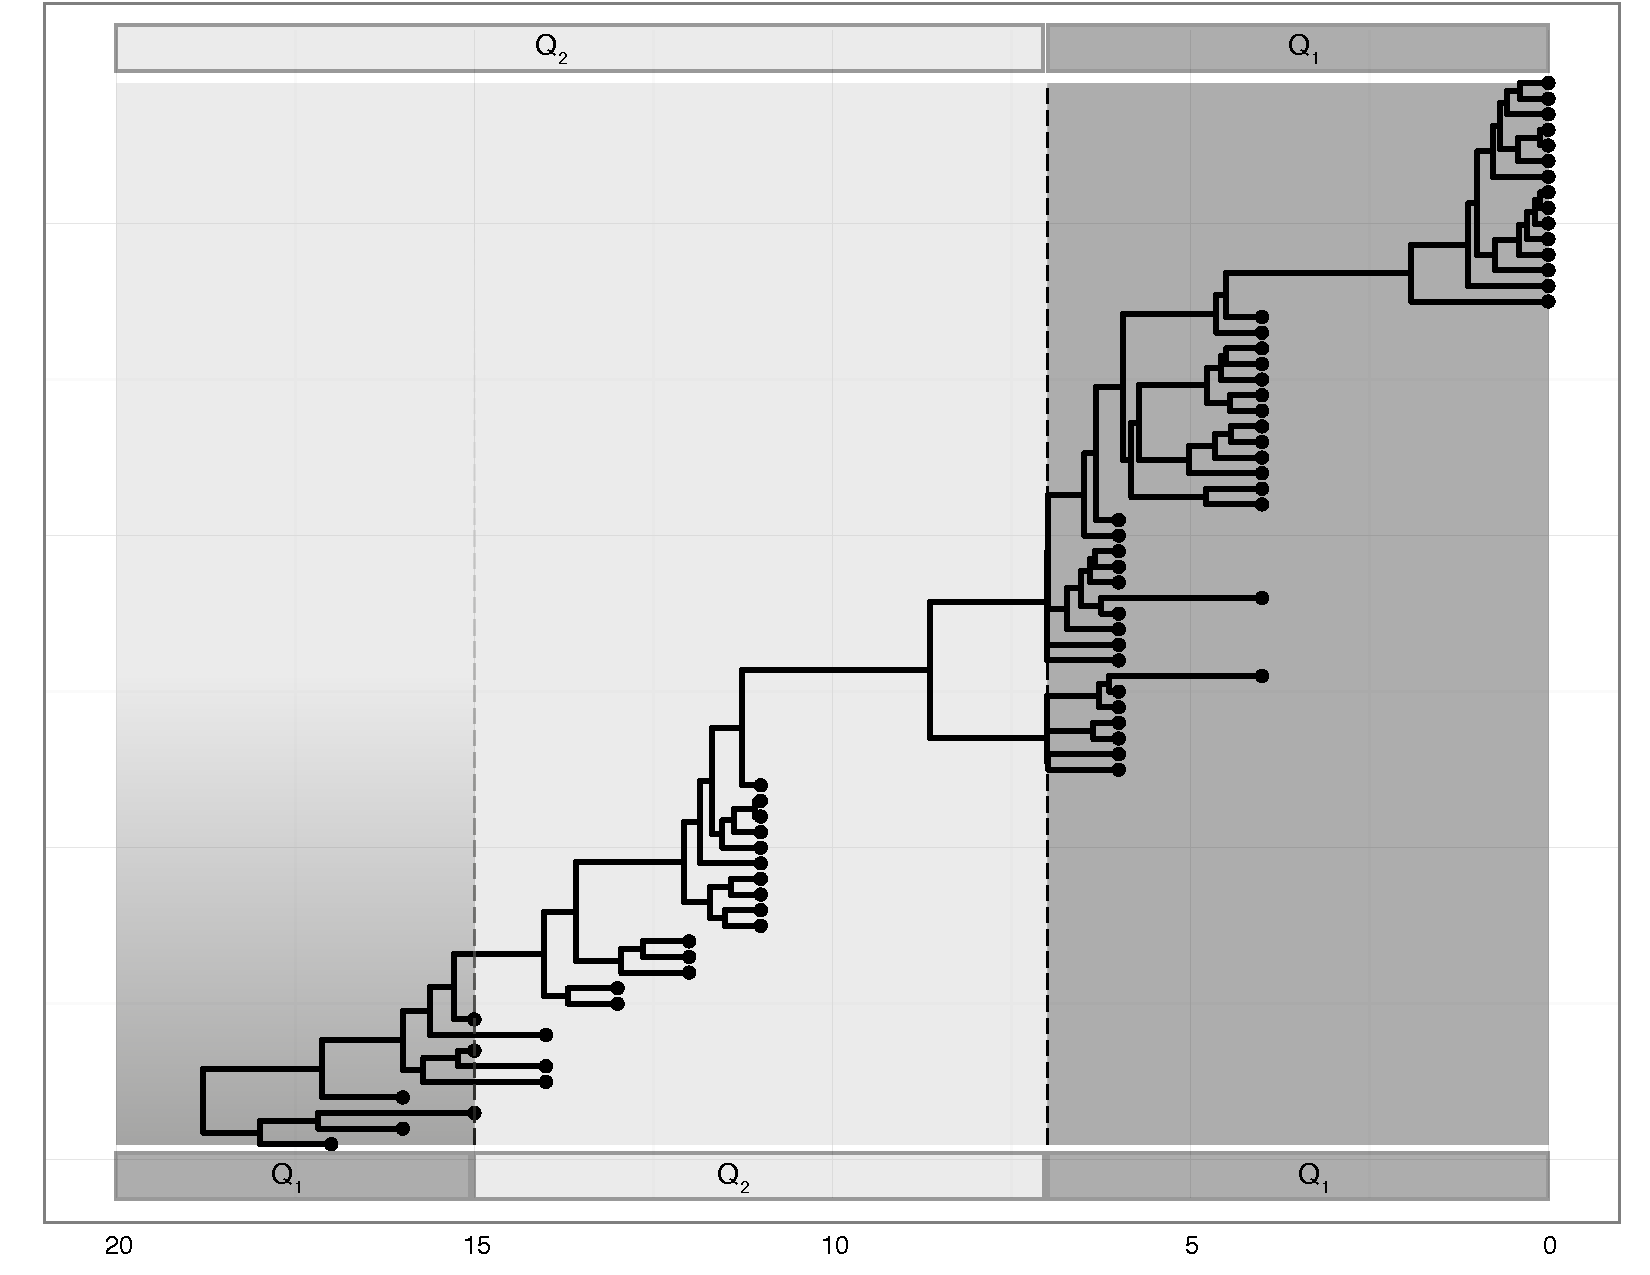
\includegraphics[scale=0.35]{treeplot} 
\caption{
{ \footnotesize 
{\bf  Epoch simulation scenarios on an influenza A maximum clade credibility tree topology.} 
% \myedit{DPeight}{
In the two-epoch example illustrated at the top with alternating grey and light grey background
% at the top, 
the transition time is set at $t_{1}=7$, creating two epochs with substitution processes governed by infinitesimal rate matrices $\mathbf{Q_{1}}$ and $\mathbf{Q_{2}}$ respectively.
The light area (one of which encompasses  two epochs in the 3-epoch scenario as indicated by the transparency gradient for the leftmost epoch) is separated from the dark grey area by a dotted line.
In the three-epoch example illustrated 
at the bottom, % at the bottom, 
the transition times are put at $t_{1}=7$ and $t_{2}=15$, creating three epochs with substitution processes governed by infinitesimal rate matrices $\mathbf{Q_{1}}$, $\mathbf{Q_{2}}$ and then again $\mathbf{Q_{1}}$, as indicated by the alternating dark and light grey areas.
% }%END: myedit
}% END: footnotesize
}%END: caption
\label{fig:2RateTree}
\end{figure}

In Figure~\ref{fig:2RateTree}, we illustrate the tree topology and the transition times defined for both a two-epoch and three-epoch specification.
This tree has 69 tips, is rooted and time-scaled, effectively covering a period of about 18 years. 
For each replicate data set, we simulate $1000$ nucleotide sites under the Hasegawa, Kishino and Yano (HKY) model \citep{hky85}. 
We set the substitution rates and base frequencies to values estimated from the real data set.
% \myedit{svtwo}{
In all our analyses of the replicate data, as well as in the analyses of the real-world data sets in the next sections, we consider the tree as random and estimate it from the nucleotide data.
% }

In a first scenario, we test whether the epoch model correctly identifies a homogeneous nucleotide substitution process. 
We simulate an alignment evolving under the HKY model with a $\kappa$ parameter (the transition-transversion bias) value of $10.0$ for the whole timespan of the tree. 
In the analyses of replicate data, we specify a boundary time $T_1=7.0$ (7 years before the most recent sampling date) creating $M=3$ ordered boundaries with $S=2$ substitution processes governing character changes between them.
We then run an MCMC chain, starting from a randomly generated tree topology and assuming proper log-normal priors on parameters $\kappa_{1}$ and $\kappa_{2}$.
We repeat the simulation and inference process $100$ times and report estimator coverage, mean (derived from the estimated values) and mean squared error (MSE) in Table~\ref{tab:Sim}.

Estimator coverage reflects the probability that the true value from which the data derive falls within the model estimated nominal 
credible interval and hence predicts the performance of the methods across a wide ensemble of data sets.
While Bayesian credible intervals do not need to yield nominal coverage, we still obtain coverages of 96\% and 98\% for $\kappa_{1}$ and $\kappa_{2}$ respectively.

In a second simulation scenario, we consider a heterogeneous substitution process in which the recent substitution history (more recent than $T_{1}=7.0$) is governed by an HKY model with $\kappa = 1.0$, and alters to an HKY model with $\kappa = 10.0$ beyond that boundary time. 
By analyzing 100 simulation replicates generated under these settings, we arrive at a coverage of 98\% for $\kappa_{1}$ and 96\% for $\kappa_{2}$.

In a third nucleotide simulation scenario, we consider $S=3$ epochs, where before time $T_{1}=7.0$ substitutions occur under an HKY model with a $\kappa$ value of $1.0$, between $T_{1}$ and $T_{2}=15.0$ under an HKY model with $\kappa=10.0$ and after $T_{2}$ again under an HKY model with $\kappa=1.0$. 
The resulting coverages are 95\%, 95\% and 89\% for $\kappa_{1}$, $\kappa_{2}$ and $\kappa_{3}$ respectively. 
As we introduce more epochs, we observe a concomitant increase in MSE.
This can be expected as partitioning the time into more intervals will typically leave corresponding epochs less informed as less branch length is located in each epoch. 
For the same value of $\kappa = 1.0$ in the three-epoch model, the MSE is somewhat higher for the oldest epoch (0.071) compared to the most recent epoch (0.021), which is also in line with more branch length informing the latter (Figure~\ref{fig:2RateTree}).

%---SIMULATION RESULTS---%
\afterpage{\clearpage
\begin{sidewaystable}
% \begin{minipage}{\textheight} 
\centering
\footnotesize{
\begin{tabular}{cccccccccccccc}
\hline 
\multicolumn{2}{c}{\textbf{Simulated}} &  & \multicolumn{11}{c}{\textbf{Estimated}}\tabularnewline
 &  &  & Coverage & Mean & MSE\footnote{Mean Squared Error} &  & Coverage & Mean & MSE &  & Coverage & Mean & MSE\tabularnewline
\hline 
\multicolumn{2}{c}{nucleotides} &  &  & $\kappa_{1}$\footnote{HKY model's transition-transversion bias parameters} &  &  &  & $\kappa_{2}$ &  &  &  & $\kappa_{3}$ & \tabularnewline
\cmidrule(lr){1-2}
\cmidrule(lr){4-6}
\cmidrule(lr){8-10}
\cmidrule(lr){12-14}
 & $\kappa_{1}=10$ &  & 0.96 & 10.068 & 1.005 &  & 0.98 & 10.283 & 1.097 &  & - & - & -\tabularnewline
dated tips & $\kappa_{1}=1$, $\kappa_{2}=10$ &  & 0.98 & 1.007 & 0.008 &  & 0.96 & 10.446 & 1.551 &  & - & - & -\tabularnewline
 & $\kappa_{1}=1$, $\kappa_{2}=10$, $\kappa_{3}=1$ &  & 0.96 & 1.010 & 0.009 &  & 0.96 & 9.993 & 2.435 &  & 0.95 & 1.017 & 0.026\tabularnewline
contemporaneous & $\kappa_{1}=1$, $\kappa_{2}=10$, $\kappa_{3}=1$ &  & 0.96 & 1.049 & 0.002 &  & 0.95 & 10.002 & 3.723 &  & 0.92 & 1.022 & 0.061\tabularnewline
\hline 
\multicolumn{2}{c}{codon} &  &  & $\omega_{1}$\footnote{Yang codon model's nonsynonymous to synonymous substitution rate ratio} &  &  &  & $\omega_{2}$ &  &  &  & $\omega_{3}$ & \tabularnewline
\cmidrule(lr){1-2}
\cmidrule(lr){4-6}
\cmidrule(lr){8-10}
\cmidrule(lr){12-14}
 & $\omega_{1}=1$ &  & 0.94 & 0.993 & 0.048 &  & 0.93 & 1.014 & 0.53 &  & - & - & -\tabularnewline
dated tips & $\omega_{1}=0.1$, $\omega_{2}=1$ &  & 0.90 & 0.103 & 0.001 &  & 0.93 & 1.011 & 0.054 &  & - & - & -\tabularnewline
 & $\omega_{1}=0.1$, $\omega_{2}=1$, $\omega_{3}=0.1$ &  & 0.92 & 0.102 & 0.001 &  & 0.89 & 1.096 & 0.274 &  & 0.96 & 0.110 & 0.02\tabularnewline
contemporaneous & $\omega_{1}=0.1$, $\omega_{2}=1$, $\omega_{3}=0.1$ &  & 0.93 & 0.100 & 0.001 &  & 0.96 & 1.067 & 0.051 &  & 0.95 & 0.103 & 0.002\tabularnewline
\end{tabular}
} % END: footnotesize
% \end{minipage}
\caption{
{ \footnotesize 
{\bf Estimator performance for simulated data sets.} 
The table lists the parameter values used to generate data in first major column and coverage of their estimates, along with measures of variance and bias, in the second major column.
Consecutive rows present the results for the first, second and third nucleotide model simulation for dated-tip samples and the third nucleotide model simulation for contemporaneous sequences (ultrametric tree), followed by the  the results of first, second and third codon model simulation for dated-tip samples and the third codon model simulation for contemporaneous sequences. 
}% END: footnotesize
}
\label{tab:Sim}
\end{sidewaystable}
\clearpage }% END: afterpage

Epoch models are not restricted to nucleotide models; they can also relax time-homogeneity in full codon substitution models, such as the Goldman-Yang (GY94) codon model \citep{Goldman1994}.
We here examine the performance of such codon models in an epoch setting. 
As before, we first test a homogeneous substitution scenario and check whether the model is able to recover homogeneous values for the $\omega$ parameters across epochs. 
To this end, we simulate $500$ nucleotide triplets under the GY94 codon model with an $\omega$ parameter value of $1.0$. 
Performing 100 simulation replicates yields a coverage of 94\% for $\omega_{1}$ and 93\% for $\omega_{2}$. 
To asses the coverage in a heterogeneous codon substitution scenario, we set the true values to $\omega_{1}=0.1$ and $\omega_{2}=1.0$, with a transition time $T_{1}=7.0$ between the epochs, which results in a coverage of 90\% and 93\% for $\omega_{1}$ and $\omega_{2}$ respectively.
We observe a somewhat higher MSE under the homogeneous scenario for $\omega_{2}$ despite the fact that we use the same value for both homogeneous and heterogeneous simulations in this case ($\omega_{2}$  = 1.0), but the coverage is the same for both simulation scenarios (93\%).
This highlights the importance of considering the uncertainty of point estimates when assessing potential differences between epoch parameters.

Analogous to the nucleotide simulations, we also asses the epoch model performance when the data are simulated over three heterogeneous epochs, with sequences evolving under the GY94 codon model with $\omega_{1}=0.1$ before $T_{1}=7.0$, then with $\omega_{2}=1.0$ and after time $T_{2}=15.0$ with $\omega_{3}=0.1$. 
We obtain a coverage of 92\%, 89\% and 96\% for $\omega_{1}$, $\omega_{2}$ and $\omega_{3}$ respectively.
Also in this case the MSE is higher for the oldest epoch compared to the most recent epoch.

For both nucleotide and codon models we also explore how well epoch parameters can be recovered from contemporaneous sequence data, without sequences sampled throughout the past epochs.
To this end,  we set all sampling dates to time $t = 0$, effectively transforming the tree topology to be ultrametric (all tips at equal distance from the root).
%, Supplementary Information).
We list the results for these simulations under the rows labeled as `contemporaneous' in Table \ref{tab:Sim}. 
The resulting coverages for contemporaneously sampled sequences are 96\%, 95\% and 92\% for $\kappa_{1}$, $\kappa_{2}$ and $\kappa_{3}$ respectively and 93\%, 96\% and 95\% for $\omega_{1}$, $\omega_{2}$ and $\omega_{3}$  respectively.
We note that the MSE is generally lower for estimates produced for the contemporaneous data because the ultrametric transformation implies that more branches inform the epochs.
% (see Supplementary Information).

%%%%%%%%%%%%%%%%%%%%%%%%
%---SHANKARAPPA DATA---%
%%%%%%%%%%%%%%%%%%%%%%%%
\subsection{Within-host HIV selection dynamics}

%FB: I changed the omega-s in plot and text to be in line with the rest of the manuscript (numbering increases from root to tips)
We re-analyze within-host HIV-1 sequence data from eight patients extensively sampled throughout infection starting close to the time of seroconversion \citep{Shankarappa1999}.
These patients have previously been classified as moderate or slow progressors based on progression time, or the time it takes for CD4+ T cell counts to drop below 200 cells/$\mu$l \citep{williamson2003}.
The data consist of \textit{env} C2V5 sequences collected over a 6 to 13.7 year period with an average of 12 time points per patient. % (see Supplementary Information). 
The original investigation of HIV-1 diversity and divergence over time in these patients reveals a consistent pattern of divergence stabilization at late-stage infection \citep{Shankarappa1999}.
This has led to two different hypotheses that may explain these patterns.
The immune relaxation hypothesis posits that the damaged immune system during the symptomatic stage leads to reduced selection pressure on the virus, which relaxes the need for fixing immune escape mutations in the viral population.
The cellular exhaustion hypothesis, on the other hand, states that the decreased target cell availability  in late-stage infection provides less opportunity for viral replication. While the former only impacts non-synonymous changes, the latter is expected to reduce both synonymous and non-synonymous rates of substitutions.

To distinguish between these hypotheses, we ask whether $\omega$
decreases at late-stage infection, as defined by the progression time for each patient. 
This rate ratio is an explicit parameter of the GY94 codon substitution model \citep{Goldman1994}, which we can extend with an epoch specification.  
For each patient, we compare a standard homogeneous model to a two-epoch specification with a separate GY94 model before and after boundary time $T_{1}$ set to progression time for that patient.
We exclude patient 11 from the original study because no sequence data are available after progression time for this patient \citep{Shankarappa1999}.
The two-epoch discretization allows estimating a separate $\omega$ parameter for the two infection stages in each patient, with $\omega_{2}$ denoting the $d_N/d_S$ ratio before progression and $\omega_{1}$ denoting the same parameter after progression.

%---SHANKARAPPA ANALYSIS RESULTS HPD---%
\begin{figure}[h!]
\centering
% \color{fgcolor}
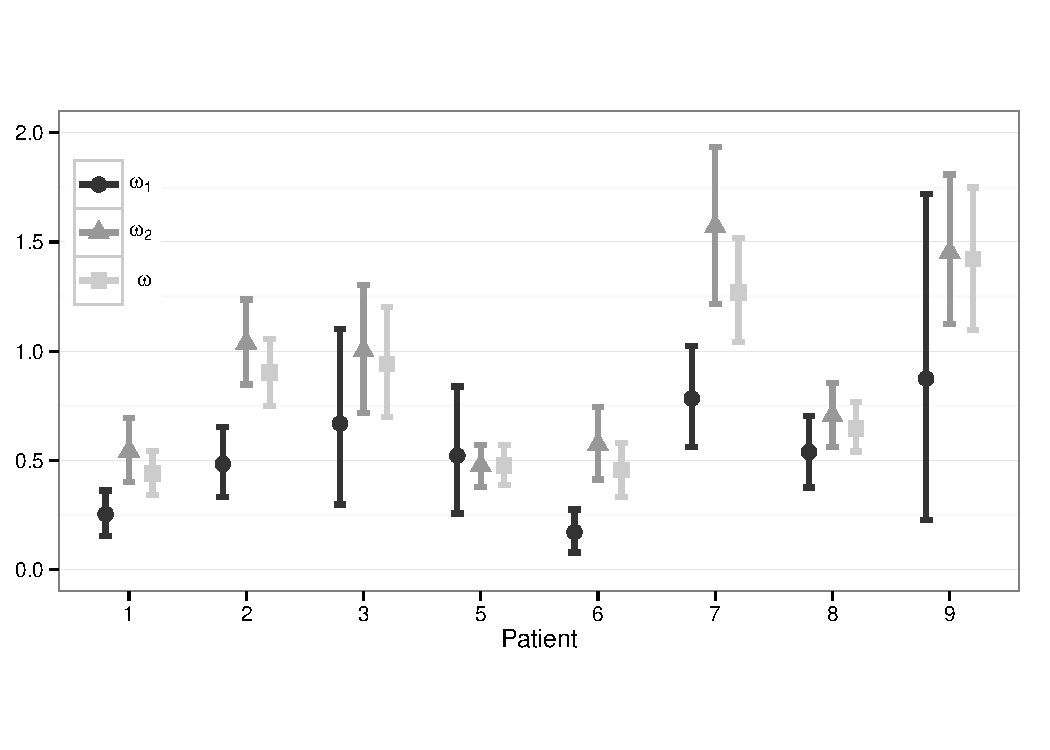
\includegraphics[scale=0.6]{shankarappa_hpd_new} 
\caption{
{ \footnotesize 
{\bf Estimates of $d_N/d_S$ ratio for within-host HIV analyses.} Vertical lines represent 95\% highest posterior density intervals for the $d_N/d_S$ ratio estimates. 
Parameter $\omega$ is estimated under the homogeneous model, while $\omega_{1}$ and $\omega_{2}$ are obtained using the epoch model.
}% END: footnotesize
}
\label{fig:shank_hpd}
\end{figure}

Figure~\ref{fig:shank_hpd} presents the results for the $\omega$ parameter estimates. 
The $\omega$ estimates indicate a general decrease in $d_N/d_S$ after progression time ($\omega_{1} < \omega_{2}$, Figure~\ref{fig:shank_hpd}).
The most pronounced differences in $\omega$ before and after progression time can be observed for patients 1, 2, 6 and 7.
For patients 2, 3, 7 and 9, the drop in mean $\omega$ estimates suggests a shift in neutral or even positive selection ($\omega_{2} \geq 1$) to negative selection ($\omega_{1} < 1 $).
The homogeneous $\omega$ estimate is generally closer to $\omega_{2}$, which can be expected because most evolutionary history takes place prior to progression time. 

%---SHANKARAPPA ANALYSIS RESULTS BF---%
\begin{table}[h!]
\centering
% \medskip
% \begin{minipage}{\textwidth} 
% \footnotesize{
\begin{tabular}%{ccc}
{@{}l*{2}{D{.}{.}{7}}@{}}
\hline 
\textbf{Patient} & \textbf{Posterior probability} & \textbf{log Bayes factor}\tabularnewline
\hline 
patient 1 & $0.999$ & $7.418$\tabularnewline
patient 2 & >$0.999$ & $9.602$\tabularnewline
patient 3 & $0.898$ & $2.174$\tabularnewline
patient 5 & $0.430$ & $-0.282$\tabularnewline
patient 6 & >$0.999$ & $9.210$\tabularnewline
patient 7 & >$0.999$ & $8.112$\tabularnewline
patient 8 & $0.933$ & $2.627$\tabularnewline
patient 9 & $0.895$ & $2.142$\tabularnewline
\hline 
\textbf{Joint evidence:} & $0.894$ & $2.14$ \tabularnewline
\end{tabular}
% } % END: footnotesize
\caption{
{ \footnotesize 
{\bf Bayes factor test for decreased selection after progression.} We report the posterior probability that $\omega_{1} < \omega_{2}$ and the corresponding Bayes factor against the alternative that $\omega_{1} \ge \omega_{2}$.
}% END: footnotesize
}
\label{tab:shank_bf}
% \end{minipage}
\end{table}

Despite the observation that the Bayesian credible intervals for patient 1, 2, 6 and 7 estimates do not overlap, this does not provide a formal test to evaluate their differences.
Therefore, we conduct a Bayes factor (BF) test \citep{Suchard2005} that expresses the posterior odds over the prior odds that $\omega_{1} < \omega_{2}$ for the individual analyses of each patient.
% To determine the posterior odds, we note that the MCMC sample average of an indicator function that the parameter values fall within one competing model space converges to the posterior probability of that model.
% \myedit{sveighteen}{
To determine the posterior odds for the hypothesis that $\omega_{1} < \omega_{2}$, we note that the MCMC sample average of an indicator function that keeps track of samples for which $\omega_{1} < \omega_{2}$ converges to the posterior probability of that hypothesis.
% }
The prior odds in our case is simply 1.
The log Bayes factors listed in Table \ref{tab:shank_bf} suggest generally strong evidence for a declining selective pressure after progression, with one notable exception for patient 5.
We also provide a Bayes factor that summarizes the joint evidence for $\omega_{1} < \omega_{2}$, which suggest an overall support in favor of the immune relaxation hypothesis (log BF = 2.14), in accordance with previous findings suggesting a general decrease in non-synonymous divergence at late-stage infection \citep{williamson2005, Lemey2007}.

%%%%%%%%%%%%%%%%%%%%%%
%---PHYLOGEOGRAPHY---%
%%%%%%%%%%%%%%%%%%%%%%
\subsection{Seasonal circulation dynamics of human influenza A}

In a second application of the epoch model, we focus on discrete diffusion processes to infer spatio-temporal history from viral gene sequences.
This type of phylogeographic inference, where the sampling locations are considered as discrete geographic traits, has gained popularity in recent years, at least partly because of a flexible and efficient Bayesian implementation that connects dispersal dynamics to sequence evolution in time-measured phylogenies \citep{Lemey2009}.
Recently \citet{Bahl2011} have applied this Bayesian inference framework to investigate the circulation dynamics of global influenza A H3N2 through time.
Since the authors were interested in capturing the heterogeneity in these dynamics over successive seasonal epidemics between 2003 and 2006, they consider discrete traits that are the product of sampling location and sampling time (epidemic season).
% \myedit{svsixteen}{
This means for example that samples collected from October 2002 to February 2003 in New York are assigned to the discrete state labelled as ``New York 2003'', while sampling in the sample location during another seasons will be represented by another state \citep{Bahl2011}.
% }
Not only does this discretization by sampling time seem counterintuitive for a model that emits discrete outcomes as a continuous function of time, it also considerably increases the dimensionality of the CTMC rate matrix and thus the number of parameters to inform by the sparse spatial data.

Here, we explore epoch time-discretization as a more appropriate alternative to detect temporal heterogeneity in influenza dispersal.
We revisit the \citet{Bahl2011} data set that consists of 525 influenza A H3N2 hemagglutinin sequences sampled from  Australia, Europe, Japan, New York, New Zealand, Southeast Asia and Hong Kong ($n=75$ each) from 2003 to 2006.
In a first epoch model extension of the discrete phylogeographic approach, we specify alternating epochs for the time intervals encompassing northern hemisphere spring and summer and the time intervals encompassing northern hemisphere autumn and winter.
The discrete diffusion parameters are shared across rate matrices for the spring and summer epochs as well as for the autumn and winter epochs, effectively producing two rate matrices compared to a single matrix for the homogeneous model. Figure~\ref{fig:2EpochFlu} schematically represents this $S=7$ epoch parameterization. 
Following \cite{KassRaftery95} we report rates that yield a Bayes factor support interpreted as `strong evidence'.

%---FLU DATA RESULTS MAP---%
\begin{figure}[h!]
\centering
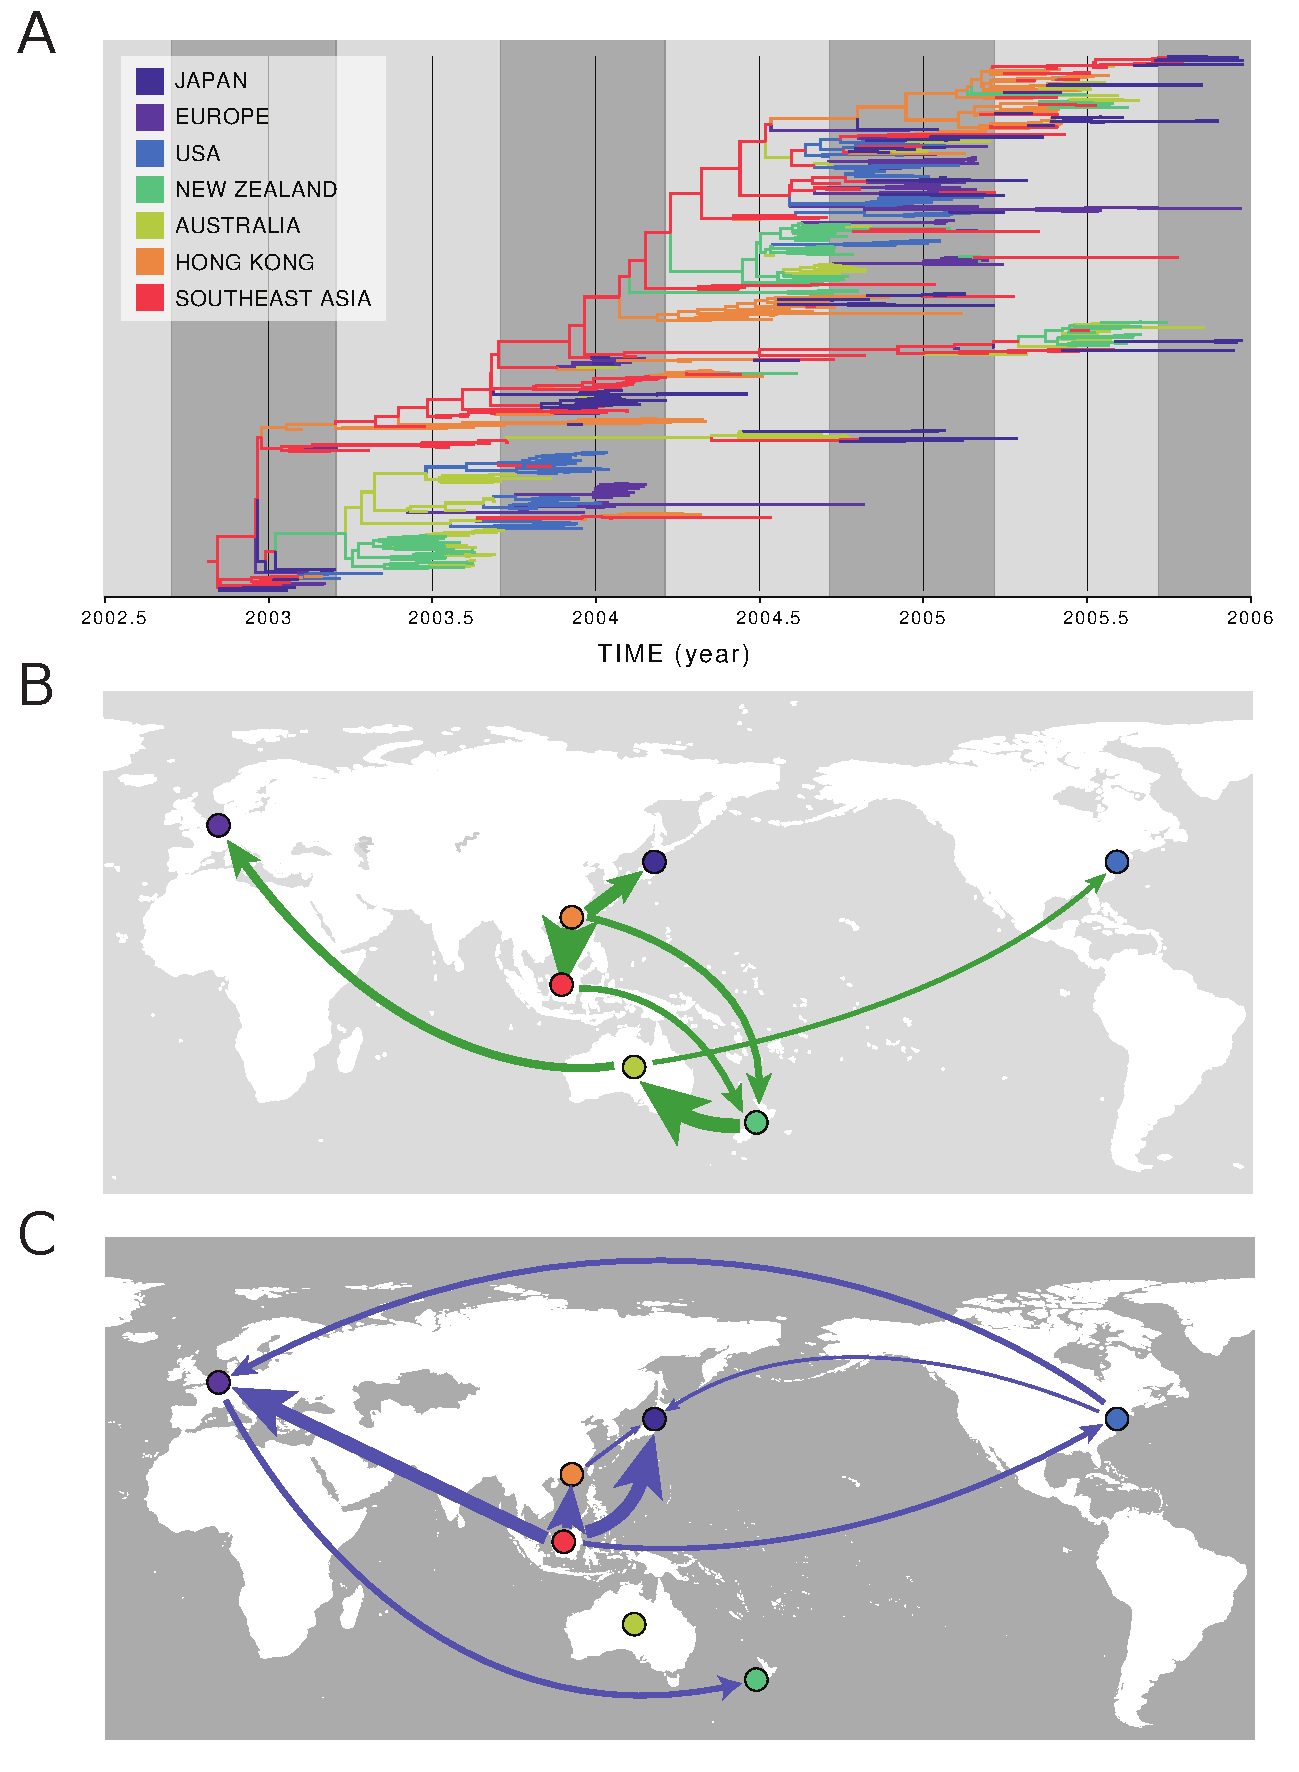
\includegraphics[scale=0.5]{flu2_epoch} 
\caption{
{ \footnotesize 
{\bf A two-epoch phylogeographic model applied to seasonal influenza H3N2.} 
A. Maximum clade credibility (MCC) tree with branches colored according to modal discrete location states at each node. The grey time intervals represent the epoch model with a single discrete rate matrix shared across northern hemisphere spring and summer (light grey) time intervals and another rate matrix shared across the northern hemisphere autumn and winter (dark grey) time intervals. B. Diffusion rates supported by a Bayes factor $>20$ for spring and summer epoch intervals. The width of the arrows reflects the magnitude of the Bayes factor support. C. Diffusion rates supported by a Bayes factor $>20$ for autumn and winter epoch intervals.
}% END: footnotesize 
}
\label{fig:2EpochFlu}
\end{figure}

We apply a Bayesian stochastic search variable selection (BSSVS) procedure to identify the best supported diffusion rates within each epoch using a Bayes factor test, as available in the SPREAD software \citep{Bielejec2011}. Rates yielding a Bayes factor over 20 are represented in Figure~\ref{fig:2EpochFlu} A\&B for the spring and summer epoch and autumn and winter epoch respectively.
This suggests seasonal dynamics with spring and summer circulation to a large extent mirroring autumn and winter circulation.
The spring and summer epoch appears to be dominated by circulation from Southeast Asia and Hong Kong to the Southern hemisphere (New Zealand), circulation within the Southern hemisphere and also circulation from the Southern to the Northern hemisphere.
During the autumn and winter epoch on the other hand, we infer mostly circulation from Southeast Asia to the Northern hemisphere, circulation within the Northern hemisphere and occasional circulation from the Northern to the Southern hemisphere,

%---FLU DATA RESULTS PS SS---%
% \afterpage{\clearpage
\begin{table}[h!]
\begin{minipage}{\textwidth} 
\centering
% \footnotesize{
\begin{tabular}{ccc}
\hline 
\multirow{2}{*}{\textbf{Model}} & \multicolumn{2}{c}{\textbf{Marginal likelihood}}\tabularnewline
 & PS\footnote{Path Sampling} & SS\footnote{Stepping Stone Sampling}\tabularnewline
\hline 
homogeneous & -827.29 & -825.07\tabularnewline
7-epoch & -806.36  & -803.40 \tabularnewline
14-epoch & -798.77  & -795.63 \tabularnewline
\end{tabular}
% } % END: footnotesize
\caption{
{ \footnotesize 
{\bf Marginal likelihood estimates.} Comparison in terms of model fit between a homogeneous model, an epoch model with time discretized into $S=7$ epochs alternating between 2 different rate matrices and an epoch model with time discretized into $S=14$ epochs, alternating between 4 separate rate matrices.
} % END: footnotesize
}
\label{tab:flu_ps}
\end{minipage}
\end{table}
% \clearpage }% END: afterpage

To evaluate the improvement of explicitly modeling these largely opposing dynamics, we compared model fit with a homogeneous model using path sampling and stepping-stone sampling, two reliable estimators of marginal likelihood \citep{Baele2012}. 
Proper priors were used for all parameters during the various analyses, as well as the model selection, since such priors have been shown to be essential when performing marginal likelihood estimation \citep{Baele2012}.
The results of the model comparison are listed in Table~\ref{tab:flu_ps} and provide evidence for the two-epoch model outperforming the homogeneous model.
When we further extend our phylogeographic epoch time-discretization to four epochs, modeling separate dynamics for each individual season, we observe additional improvements in terms of marginal likelihoods but with diminishing returns with respect to the two-epoch vs. homogeneous comparison. %(see Supplementary Information for a visual summary of well supported circulation rates in each season).

%---RUN TIME ANALYSIS---%
\subsection{Run time analysis}

To investigate the speed increase offered by a parallel execution of different tasks, we measure the speed-up relative to serial execution of both update and convolution operations for the analyses of two empirical data sets.
We perform our analyses on a standard desktop PC equipped with Intel 2$^{\text{nd}}$ Gen Core i7 2 i7-2600K / 3.9 GHz CPU and 16 GB of DDR3 SDRAM along with a NVIDIA GeForce GTX 590 card, carrying two GPU devices with a total of 1024 CUDA cores, running at 1215 MHz and 1536MB of memory per GPU. 

%---STACK SIZE TIMING---%
\begin{figure}[h!]
\centering
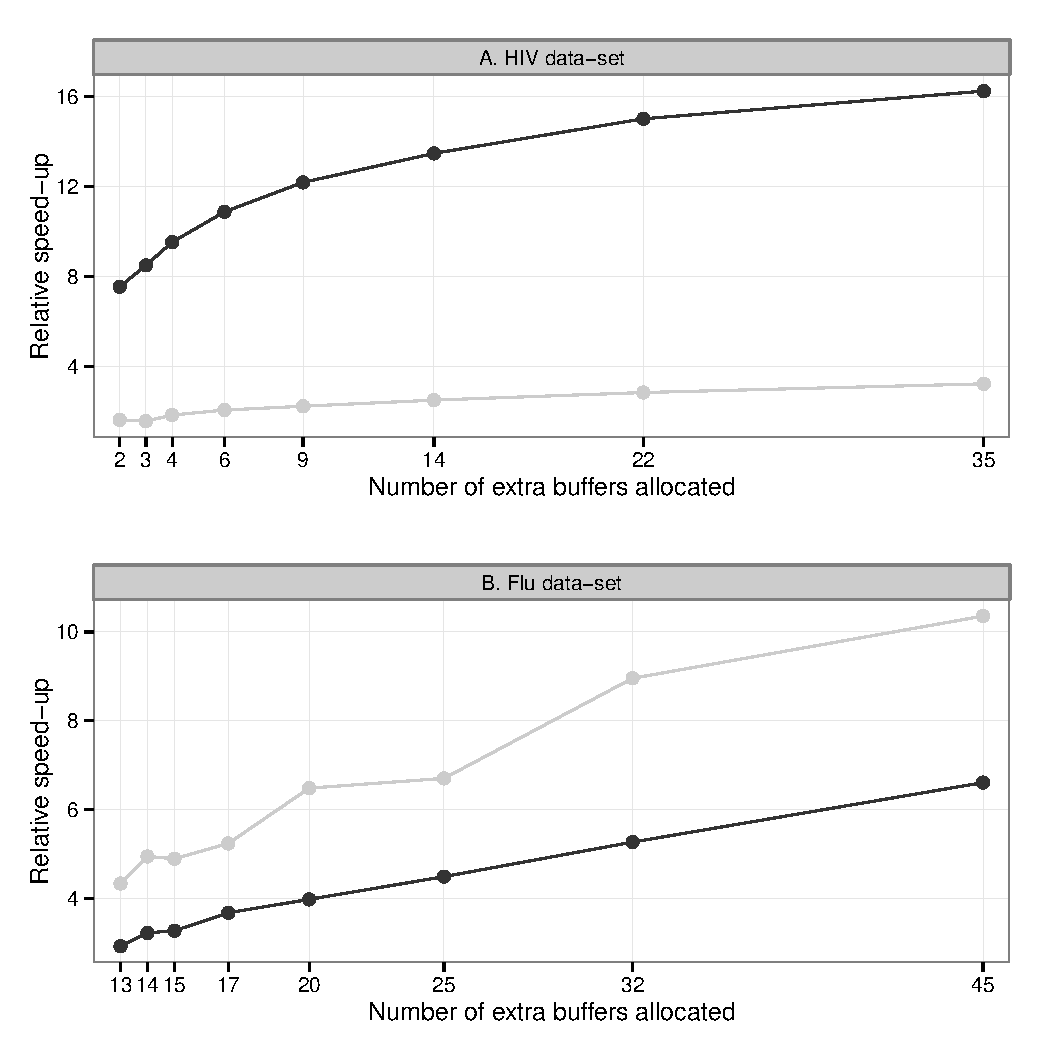
\includegraphics[scale=0.6]{timing} 
\caption{
{\footnotesize 
{\bf Relative speed-ups as a function the number of extra buffers allocated for two real data examples.}
Speed-ups are reported relative to the serial execution, using system time spent sampling 1,000,000 states from the posterior distribution using an MCMC sampler. 
Black dots denote update transition matrices operations, grey dots denote convolve operations.
A. Speed-ups for a flu data set (522 taxa, discrete geographic diffusion process between $K=7$ states, time discretized into $S=13$ epochs, see {\it{Seasonal circulation dynamics of human influenza A}}). 
B. Speed-ups for a patient 3 from HIV data set (109 taxa, 516 sites, state-space size of $K=61$ codons, $S=2$ epochs, see {\it{Within-host HIV selection dynamics}}). 
} % END: footnotesize 
}
\label{fig:StackSizeTiming}
\end{figure}

Figure~\ref{fig:StackSizeTiming} presents the GPU speed-ups induced by different choices of the number of extra buffers, which in turn determine the queue size for update and convolve operations. 
The leftmost points correspond to the minimum number of extra buffers we can allocate; speed-ups are reported relative to the serial execution of the convolve and update steps on a CPU device. We perform our analyses with double floating point precision on both the GPU and CPU.
We note that the speed-ups between data sets depend not only on the number of epoch transition times, but also importantly on the actual number of convolution operations performed during the tree topology traversal and this is tree-dependent. 
The convolution step for the influenza example emerges as the most time consuming part of the routine (Figure~\ref{fig:StackSizeTiming} AB), as many branches intersect multiple epochs, breeding multiple calls to the \emph{ConvolveTransitionMatrices} BEAGLE kernel.  
For the codon-based HIV-1 example (Figure~\ref{fig:StackSizeTiming} A) a large state space alongside with a modest number of branches intersecting epoch transition boundaries provide the main reason why we witness a significant amount of time being spent computing finite-time transition probabilities. 
% As for all the HIV-1 data sets we also compare sequential and parallel absolute timings for an `epochized' codon model, measured by the time it takes MCMC chain to sample 1 million posterior samples (see the Supplementary Information).


\section{Discussion and Conclusions}

\citet{Goode2008} demonstrate that a change in evolutionary pattern affecting all individuals of a population can be modeled by specifying different substitution models across different time intervals rather than over different lineages.
Here, we extend this approach and further demonstrate how epoch modeling can uncover temporal heterogeneity in discrete character evolution in phylogenetic histories.
We are mainly interested in heterogeneity resulting from variation in the relative intensities of substitutions across time and not heterogeneity induced by nonstationarity.
We embed the epoch model in a Bayesian phylogenetic framework that focuses entirely on time-measured trees and integrates over all plausible evolutionary histories for the observed sequence data.
Our simulations show that the model is able to recover different scenarios of heterogeneity under different substitution models, but epoch parameters can also reflect an underlying process that is in fact homogeneous, thus avoiding false positives (see Table~\ref{tab:Sim}).
Following \citet{Goode2008}, we primarily focus on time-stamped sequence data from rapidly evolving pathogens for which the ecological and evolutionary dynamics occur on the same time scale and potentially interact.
However, our approach does not necessarily require sequence data sampled throughout different epochs.
In fact, the simulation study demonstrates that the epoch model can also capture time-heterogeneity in the substitution process inferred from contemporaneous sequence data. 
In this case, the amount of evolutionary history, as measured by branch length within each epoch, determines how accurately epoch parameters can be inferred.

We apply our model both in the context of sequence evolution and spatial dispersal dynamics.
For the former, we focus on within-host HIV-1 evolution and explicitly test different hypotheses that explain the stabilization in sequence divergence in late-stage infection \citep{Shankarappa1999}.
This phenomenon has been attributed to weakened selection pressure (immune relaxation) or to a decrease in average viral replication rate (cellular exhaustion) \citep{williamson2005}.
Various studies have attempted to distinguish between both scenarios by contrasting the accumulation of non-synonymous and synonymous  substitutions using different methodologies \citep{williamson2005,Lemey2007,Lee2008}.
While two studies provide strong support for the immune relaxation hypothesis using different methodologies \citep{williamson2005,Lemey2007}, \citet{Lee2008} suggest that both synonymous and non-synonymous evolutionary rates decline as disease progresses.
Here, we explicitly model a change in the $d_N/d_S$ ratio in codon substitution models while integrating over the underlying within-host HIV-1 phylogeny, and formally evaluate the support for a decrease in $d_N/d_S$ using Bayes factors. 
This demonstrates strong overall support in favour of the immune relaxation hypothesis.

Although the hypothesis we test here does not require investigating site-specific selection patterns, we note that codon models that accommodate different categories of sites also have interesting applications in the epoch framework.
This has been demonstrated by \citet{Goode2008}, who employed a particular codon parameterization to allow for sites to switch among a neutrally evolving class, a class of negatively selected sites and a class of positively selected sites (cfr. M2, \citet{NY98}) before and after the start of HIV-1 antiretroviral therapy.
Using this approach, the authors showed that a considerable number of sites, which are identified as neutral under a time-homogenous model, are under some form of selection in one of the two epoch time periods, implying that neutrality may be context-dependent.
Codon models that accommodate different categories of sites have not yet been implemented in BEAST, at least partly because they are computationally prohibitive.
Incorporating such models in an epoch approach would contribute even more to the computational burden.
We hope however that the parallel implementations we pursue here may still allow practitioners to explore such extensions in future research. %

Our second application exemplifies  the use of epoch time-discretization in phylogeographic inferences that consider sampling locations as discrete traits.
In particular, we demonstrate how epoch modeling can capture seasonality in human influenza A H3N2 circulation dynamics, without the need to complicate location traits with sampling time.
Based on a data set previously analyzed by \citet{Bahl2011}, we infer different epidemiological connections between the northern hemisphere spring-summer epoch and the autumn-winter epoch.

In both cases Southeast Asia (and Hong Kong) appear to play a central role in seeding the seasonal epidemics in the different hemispheres (Figure~\ref{fig:2EpochFlu}). 
However, we remain cautious in interpreting the support for diffusion rates in the context of source-sink dynamics because strong evidence for such a rate being non-zero does not necessarily imply that the diffusion rate itself is high \citep{Faria2013}.
For example, the connection we identify between Europe and New Zealand during the northern hemisphere autumn and winter epidemic may represent a few introductions into New Zealand without extensive onwards transmission.
Therefore, it remains difficult to assess which rates govern potential source-sink dynamics.

The specification of two alternating epochs yields a better model fit than a homogeneous model while providing a more parsimonious parameterization compared to the use of discrete traits that are based on both sampling location and epidemic season as in \citet{Bahl2011}.
Model fit differences are more readily detected in this application because an additional epoch adds an entirely new set of parameters.
Incorporating more epochs further increased model fit (Table~\ref{tab:flu_ps}), albeit with diminishing returns, but it is clear that there are limits to the flexibility that can be incorporated in phylogeographic reconstructions, which represent inherently data-sparse inferences.
In this respect, it is interesting to note that approaches are available to share information across epochs while still allowing for the detection of differences among them \citep{Suchard2003b}.
This can be achieved by specifying hierarchical priors, both on standard rate parameters \citep{Edo-Matas2011} as well as, more recently, on the rate indicators in a BSSVS procedure \citep{Cybis2013}.
Assuming that phylogeography represents a major application for the epoch model, further research is needed to explore these approaches as well as other sparse parameterizations of discrete dispersal processes.

The two data sets we examine represent examples with clear \textit{prior} hypotheses that correspond to fixed transition times.
It may also be of interest to apply the model when the transition times are unknown. 
Although it would be straightforward to estimate the time of a fixed number of epoch transition in our MCMC framework, estimating the number of epochs may be more challenging.
However, our previous experience with change-point processes in phylogenetics \citep{Suchard2003a} suggests that it should be possible to introduce prior distributions over these quantities and jointly infer them when uncertainty remains in their specification.
Instead of trying to identify the most appropriate discretization of time, one may potentially use epoch modeling to approximate more complex functions of time.
\citet{Rodrigo2008} outline two approaches to allow rate matrices to vary as a function of time, one of which approximates that function by partitioning time into a fine grid of intervals.
This is likely to be a computationally expensive avenue, but its performance will mostly depend on the availability of dense sampling throughout time \citep{Rodrigo2008}.%

An interesting direction for further research using the epoch model is to couple epoch-specific parameters to external covariates.
For the within-host HIV data sets we analyze here, it may be interesting to ask whether $\omega$ varies with changes in CD4+ counts or viral load.
In our Bayesian framework, we can address this question through formulating a hierarchical phylogenetic model \citep{Edo-Matas2011} over the epoch-specific parameters, considering the covariates as fixed-effects. 
We can further estimate the posterior probabilities of all possible linear models that may or may not include the covariates using Bayesian stochastic search variable selection \citep{Kuo1998}.  
In addition to external covariates, we can also consider connecting the evolutionary parameters in an epoch model to population size parameters in non-parametric models of population size change through time, such as the Bayesian skyline \citep{Drummond2005}, skyride \citep{Minin2008b} and skygrid models \citep{Gill2013}.

By adding an additional layer of complexity to our evolutionary models and inference framework, we further increase the computational demands in a field that is already computationally intensive. 
Our Bayesian approach integrates over all possible evolutionary scenarios, which is challenging for a large number of sequences even when specifying the simplest of evolutionary models.
To mitigate the additional burden imposed by our epoch time-discretization and the operations involved, we have implemented our model in the high-performance BEAGLE library allowing us to perform the calculations on GPU architectures.
Although this has proven extremely useful, in particular for large state-space models such as codon substitution models \citep{Suchard2009}, more research is needed to further stretch the limits of practical computational restrictions.
 
In summary, our work has extended the phylodynamic framework with a model that is capable of quantifying and testing temporal heterogeneity in discrete state transition processes, which is proving useful to detect changing selective dynamics in rapidly evolving viral populations as well as fluctuations in historical circulation dynamics.



\cleardoublepage
\chapter{Visualizing viral spread in time and space\label{chap:spread}}

\begin{remark}{Outline}
This chapter is adapted from the following publication: \\
F. Bielejec, A. Rambaut, M.A. Suchard and P. Lemey.
SPREAD: spatial phylogenetic reconstruction of evolutionary dynamics.
Bioinformatics, 2011, 27(20): 2910 -- 2912
\end{remark}

\section{Abstract}

\textbf{Summary:}\\
SPREAD is a user-friendly, cross-platform application to analyze and visualize Bayesian phylogeographic reconstructions incorporating spatial-temporal diffusion.
The software maps phylogenies annotated with both discrete and continuous spatial information and can export high-dimensional posterior summaries to keyhole markup language (KML) for animation of the spatial diffusion through time in virtual globe software.
In addition, SPREAD implements Bayes factor calculation to evaluate the support for hypotheses of historical diffusion among pairs of discrete locations based on Bayesian stochastic search variable selection estimates.
SPREAD takes advantage of multi-core architectures to process large joint posterior distributions of phylogenies and their spatial diffusion and produces visualizations as compelling and interpretable statistical summaries for the different spatial projections.\\

\noindent
\textbf{Availability:} \\
SPREAD is licensed under the GNU Lesser GPL and its source code is freely available as a GitHub repository: \url{https://github.com/phylogeography/SPREAD} 
Compiled, runnable package and supplementary data are hosted at: \url{http://rega.kuleuven.be/cev/ecv/software/spread} 

\begin{figure}[H]
\centering
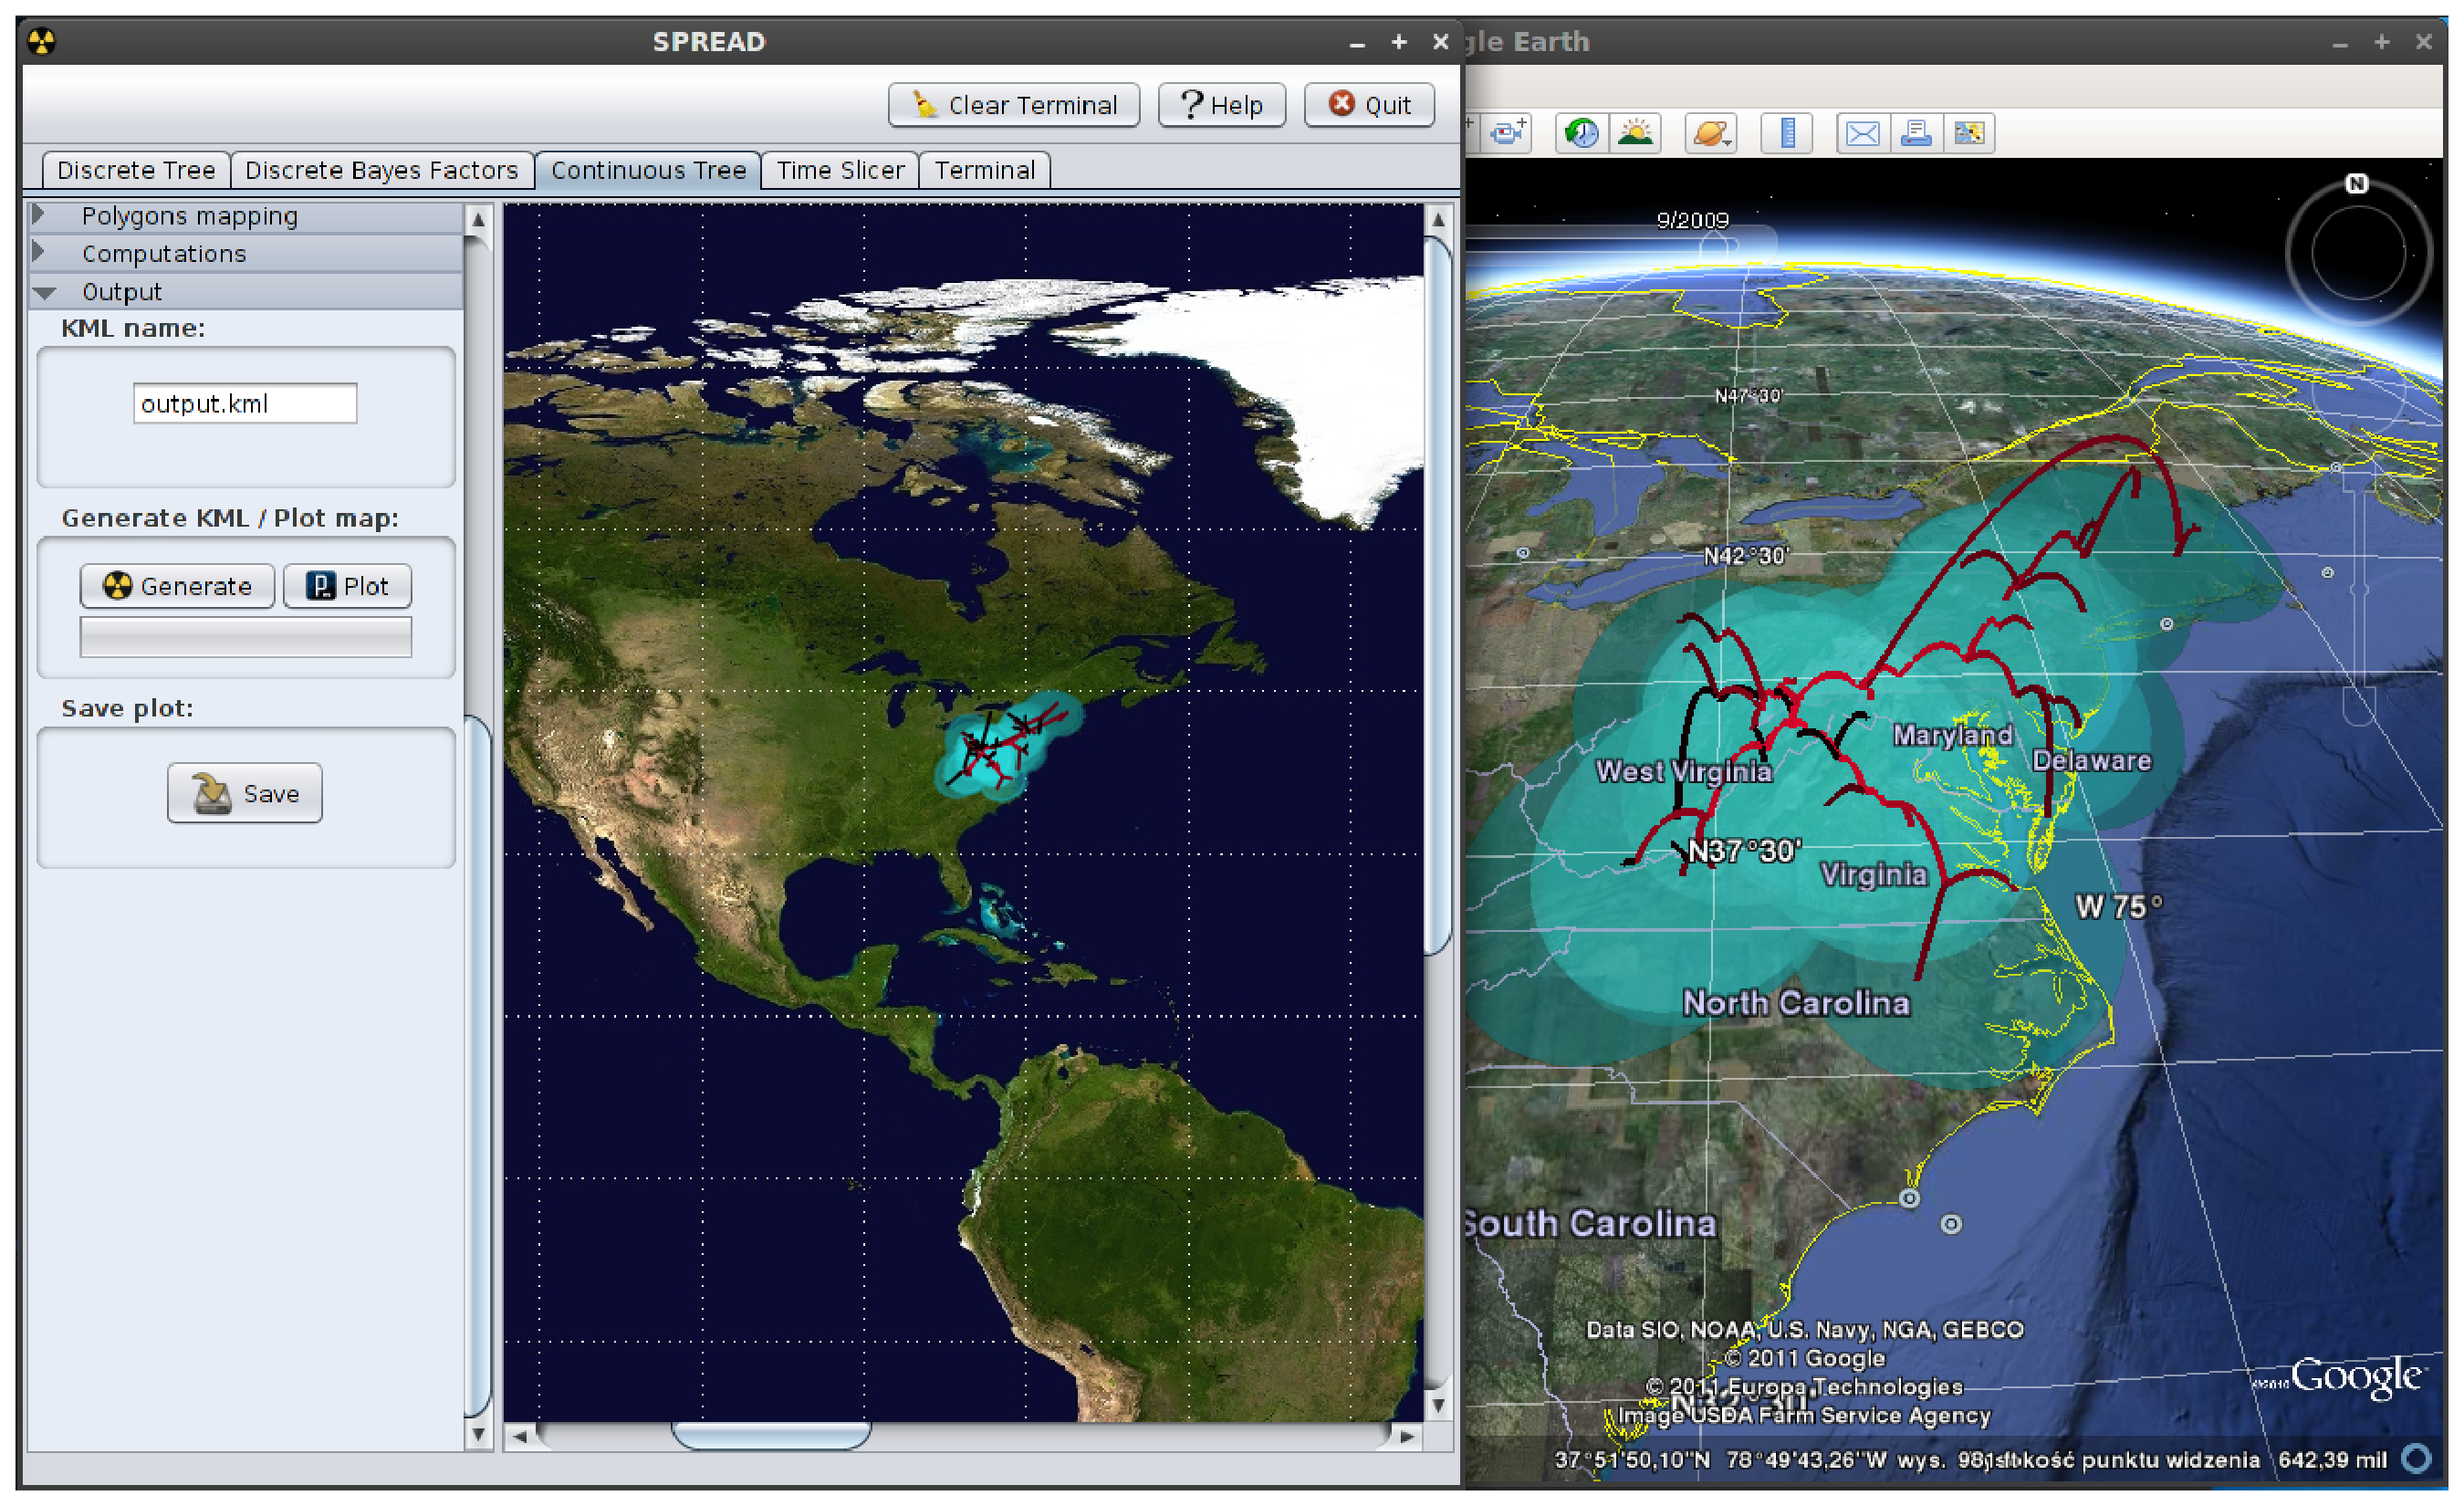
\includegraphics[scale=0.25]{RacRABV_cont_vis}
\caption{
{ \footnotesize 
{\bf Screenshot of SPREAD.}
This example visualizes the phylogeographic history of rabies among raccoons along the Eastern US seaboard under a continuous diffusion model.  Such visualizations allow users to quickly inspect key evolutionary changes in their geographic context.  Further generation of KML output enables interactive exploration in the time-dimension as well in freely available virtual globe software, such as {\sc Google Earth} (on right).
}% END: footnotesize 
}
\label{fig:01}
\end{figure}

\section{Introduction}

The advent of powerful and flexible Geographic Information Systems (GIS) has fostered an increasing interest in incorporating geographical information into molecular phylogenetic methods.
Spatial phylogenetic projections in a cartographic background play an important role in these developments \citep{Kidd2006, Parks2009}, but most applications remain limited to mapping phylogenetic tip taxa to their geographical coordinates.
Mapping phylogeographic histories of geo-referenced taxa requires a robust statistical estimate of the geographic locations at the ancestral nodes of the tree. 
To obtain such estimates under stochastic process-driven models, we recently proposed a suite of Bayesian inference approaches for the joint reconstruction of evolutionary and geographic history \citep{Lemey2009,Lemey2010, Bloomquist2010}.
Models that accommodate spatial diffusion in discrete and continuous space have been implemented in a flexible Bayesian statistical framework (BEAST, \cite{Drummond2007}, \url{http://beast.bio.ed.ac.uk}) for hypothesis testing based on time-measured evolutionary histories.
These approaches produce statistical distributions of temporal-spatial phylogenies and this has created new challenges for statistical phylogenetics in producing informative and compelling visualizations.
Here, we present software to fully exploit spatio-temporal annotations on phylogenies by providing flexible visual summaries that can be further examined in an interactive manner using GIS or virtual globe software. 

\section{Features}

SPREAD provides four templates to analyze and visualize different aspects of phylogeographic diffusion, labeled: \textbf{Discrete Tree}, \textbf{Discrete Bayes Factors}, \textbf{Continuous Tree} and \textbf{Time Slicer}.
The discrete and continuous tree templates typically provide posterior summaries of diffusion from a Bayesian analysis along a high-probability tree, such as the maximum clade credibility (MCC) tree of BEAST. 
However, SPREAD is not necessarily limited to this input, as it employs a general, trait-annotated NEXUS format; we provide several tree file examples in the supplementary information for both discrete or continuous annotations. 
SPREAD supports customized visualization of spatially-mapped trees, including branch coloring according to time and branch width manipulation.

\textbf{Discrete Tree} associates geographic coordinates with the discrete location states annotated to tree nodes and projects branches that accommodate location changes on a map.
Branches that maintain a location state are visualized using customizable circular polygons.

\textbf{Discrete Bayes Factors} summarizes the data support for each pairwise rate of diffusion between locations based on Bayesian stochastic search variable selection estimates inferred using BEAST.
This template takes as input a posterior sample of rate indicators from an augmented continuous-time Markov chain model and the Poisson prior specifications for the total number of non-zero rates.
\cite{Lemey2009} describe the Bayes factor calculations in more detail.

\textbf{Continuous Tree} maps all branches of a continuous diffusion phylogeography and allows plotting the uncertainty of geographic coordinates at the internal nodes through their annotated highest posterior density contours.

\textbf{Time Slicer} supplements the visualization of geographic locations estimated using continuous diffusion by summarizing the rate and degree of geographical movement over the complete posterior distribution of trees.
To obtain such ranges, we slice each rooted tree in the posterior sample at a number of points within a time interval, usually defined by the length of a summary (MCC) tree, and impute the unobserved ancestral locations for each branch that intersects those time points. To fully accommodate the uncertainty of the original inference, the imputation involves building Brownian bridges that can take into account branch-specific scaling factors of diffusion rates under relaxed random walks \citep{Lemey2010}. For each time point, we collect the imputed locations across the posterior distribution and use bivariate kernel density estimates to plot the highest posterior density contours.
The kernel density estimation follows \cite{Snyder1978} and uses bivariate normal kernels with a diagonal bandwidth with bandwidths based on Silverman's ``rule-of-thumb''  plug-in value \citep{Silverman1986}.

\section{Example and perspectives}

For all four template analyses, SPREAD offers direct visualization but also can export the mapped objects to a keyhole markup language (KML) file suitable for viewing with virtual globe software, such as Google Earth (\url{http://earth.google.com}).
A limited example on raccoon rabies diffusion \citep{Lemey2009} finds itself in Figure~\ref{fig:01};
dynamic visualizations of this example as well as others are provided at \url{http://rega.kuleuven.be/cev/ecv/software/spread}.
KML files can be imported and visualized by many GIS software packages, including ARCGIS and Cartographica.  

SPREAD is generally not the run-time limiting analysis, compared to fitting the original phylogenetic model, and readily accommodates larger problems.
Even for Bayesian phylogenetic analyses, 1000s of pathogen sequences can be accommodated, e.g. \cite{Rambaut2008}, and new computational technologies are actively stretching these limits \citep{Suchard2009}.
Future developments of SPREAD are aimed at extending built-in rendering functionality such as parsing custom base-maps and adding mouse-driven camera support to the embedded renderings. \cleardoublepage
\chapter{Evolutionary simulation\label{chap:pibuss}}

\begin{remark}{Outline}
This chapter is adapted from the following publication: \\
% F. Bielejec, A. Rambaut, M.A. Suchard and P. Lemey
F. Bielejec, P. Lemey, L. Carvalho, G. Baele, A. Rambaut, and M.A. Suchard.
\bussname: a parallel BEAST/BEAGLE utility for sequence simulation under complex evolutionary scenarios.
BMC Bioinformatics, 2014, 15(133)
\end{remark}

\section{Abstract}
        
\textbf{Background:} \\
Simulated nucleotide or amino acid sequences are frequently used to assess the performance of phylogenetic reconstruction methods.
BEAST, a Bayesian statistical framework that focuses on reconstructing time-calibrated molecular evolutionary processes,
supports a wide array of evolutionary models, but lacked matching machinery 
for simulation of character evolution along phylogenies. \\

\noindent
\textbf{Results:} \\
We present a flexible Monte Carlo simulation tool, called {\bussname}, that employs the BEAGLE high performance library for phylogenetic computations to rapidly generate large sequence alignments under complex evolutionary models.
{\bussname} sports a user-friendly graphical user interface (GUI) that allows combining a rich array of models across an arbitrary number of partitions. 
A command-line interface mirrors the options available through the GUI and facilitates scripting in large-scale simulation studies.
{\bussname} may serve as an easy-to-use, standard sequence simulation tool, but the available models and data types are particularly useful to assess the performance of complex BEAST inferences.
The connection with BEAST is further strengthened through the use of a common extensible markup language (XML), allowing to specify also more advanced evolutionary models.
To support simulation under the latter, as well as to support simulation and analysis in a single run, we also add the {\bussname} core simulation routine to the list of BEAST XML parsers.\\

\noindent
\textbf{Conclusions:} \\
{\bussname} offers a unique combination of flexibility and ease-of-use for sequence simulation under realistic evolutionary scenarios. 
Through different interfaces, {\bussname} supports simulation studies ranging from modest endeavors for illustrative purposes  to complex and large-scale assessments of evolutionary inference procedures.
Applications are not restricted to the BEAST framework, or even time-measured evolutionary histories, and {\bussname} can be connected to various other programs using standard input and output format. \\

\noindent
\textbf{Availability and requirements:} \\
The parallel BEAST/BEAGLE utility for sequence simulation is licensed under the GNU Lesser GPL and its source code is freely available as part of the BEAST Google Code repository: \url{www.code.google.com/p/beast-mcmc/}
Compiled, runnable packages targeting all major platforms along with a tutorial and supplementary data are hosted at:
\url{www.rega.kuleuven.be/cev/ecv/software/pibuss}.
The tutorial is also included as Appendix~\ref{app:pibuss_tuto}.
{\bussname} requires Java runtime environment version 1.5 or later to run its executables and the BEAGLE library to be present and configured to fully utilize its capabilities.
Bayesian Evolutionary Analysis by Sampling Trees (BEAST) is a cross-platform program for Bayesian inference in evolution and phylogenetics using molecular sequences. 
The current stable release can be obtained from \url{www.beast.bio.ed.ac.uk}.
The Broad-platform Evolutionary Analysis General Likelihood Evaluator (BEAGLE) library is free, open-source software licensed under the GNU LGPL. Both the source code and binary installers are available from \url{www.code.google.com/p/beagle-lib}. 
Scripts and input files required for repeating the simulation study presented in {\bf{Example application}} are hosted at \url{www.github.com/phylogeography/DeepRoot}.

\section{Background}

Recent decades have seen extensive development in phylogenetic inference, resulting in a myriad of techniques, each with specific properties concerning
evolutionary model complexity, inference procedures and performance both in terms of speed of execution and estimation accuracy.
With the development of such phylogenetic inference methods comes the need to synthesize evolutionary data in order to compare estimator performance and to characterize strengths and weaknesses of different approaches (e.g. \cite{Arenas2012}, \cite{Hoban2011}).
Whereas the true underlying evolutionary relationships between biological sequences are generally unknown,
Monte Carlo simulations allow generating test scenarios while controlling for the evolutionary history as well as the tempo and mode of evolution. 
This has been frequently used to compare the performance of tree topology estimation (e.g. \cite{Stamatakis2005}), but it also applies to evolutionary parameter estimation and ancestral reconstruction problems (e.g. \cite{Blanchette2008}).
In addition, Monte Carlo sequence simulation has proven useful for assessing model adequacy (e.g. \cite{Brown2009}) and for testing competing evolutionary hypotheses (e.g. \cite{Goldman1993}).
It is therefore not surprising 
that several general sequence simulation programs have been developed (e.g. Seq-Gen \cite{Rambaut1997}), but also inference packages that do not primarily focus on tree reconstruction, such as PAML \cite{PAML} and HyPhy \cite{HyPhy}, maintain code to simulate sequence data under the models they implement.

As a major application of phylogenetics, estimating divergence times from molecular sequences requires an assumption of roughly constant substitution rates throughout evolutionary history \citep{Zuckerkandl1962}. 
Despite the restrictive nature of this molecular clock assumption, its application in a phylogenetic context has profoundly influenced modern views on the timing of many important events in evolutionary history \citep{Arbogast2002}. 
Following a long history of applying molecular clock models on fixed tree topologies, the Bayesian Evolutionary Analysis by Sampling Trees (BEAST) package \citep{Drummond2012} fully integrates these models, including more realistic relaxed clock models \citep{Drummond2006,Drummond2010}, in a phylogenetic inference framework.
Despite its popularity this framework has lacked a flexible and efficient simulation tool.
Here, we address this pitfall by introducing a parallel BEAST/BEAGLE utility for sequence simulation ({\bussname}) that integrates substitution models, molecular clock models, tree-generative (coalescent or birth-death) models and trait evolutionary models in a modular fashion, allowing the user to simulate sequences under different parameterizations for each module.

{\bussname} readily 
incorporates the temporal dimension of evolution through the possibility of specifying different molecular clock model.
Further, many models and data types available for BEAST inference are matched by their simulation counter-parts in {\bussname}, including
relatively specific processes, such as for discrete phylogeography with rate matrices that can be sparse or non-reversible \cite{Lemey2009} that are generally beyond the scope of most sequence simulation tools.
The BEAST-{\bussname} connection is further reinforced by the fact that {\bussname} can easily generate simulation specification in XML format for BEAST.
Finally, we implement the core simulation routine within the BEAST code-base to ensure a shared XML syntax between the two packages and to allow for joint simulation and inference analysis using a single input file.

\section{Implementation}

Through different implementations, we support several sequence simulation procedures that balance between ease-of-use and accessibility, to model complexity.
On the one hand, the core simulation routine can be performed following specifications in an XML input file that is understood by BEAST (Figure~\ref{fig:screenshot} A).
This procedure provides the most comprehensive access to the {\bussname} arsenal of models, but may require custom XML editing.
On the other hand, {\bussname} also represents a stand-alone package that conveniently wraps the simulation routines in a user-friendly graphical user interface (GUI), allowing users to set up and run simulations by loading input, selecting models from drop-down lists, setting their parameter values, and generating output in different formats (Figure~\ref{fig:screenshot} B).
To facilitate scripting, {\bussname} is further accessible through a command-line interface (CLI), with options that mirror the GUI.
The simulation routines are implemented in Java and interface with the Broad-platform Evolutionary Analysis General Likelihood Evaluator (BEAGLE) high-performance library \cite{Ayres2012} through its application programming interface (API) for computationally intensive tasks. 

\begin{figure}[h!]
\centering
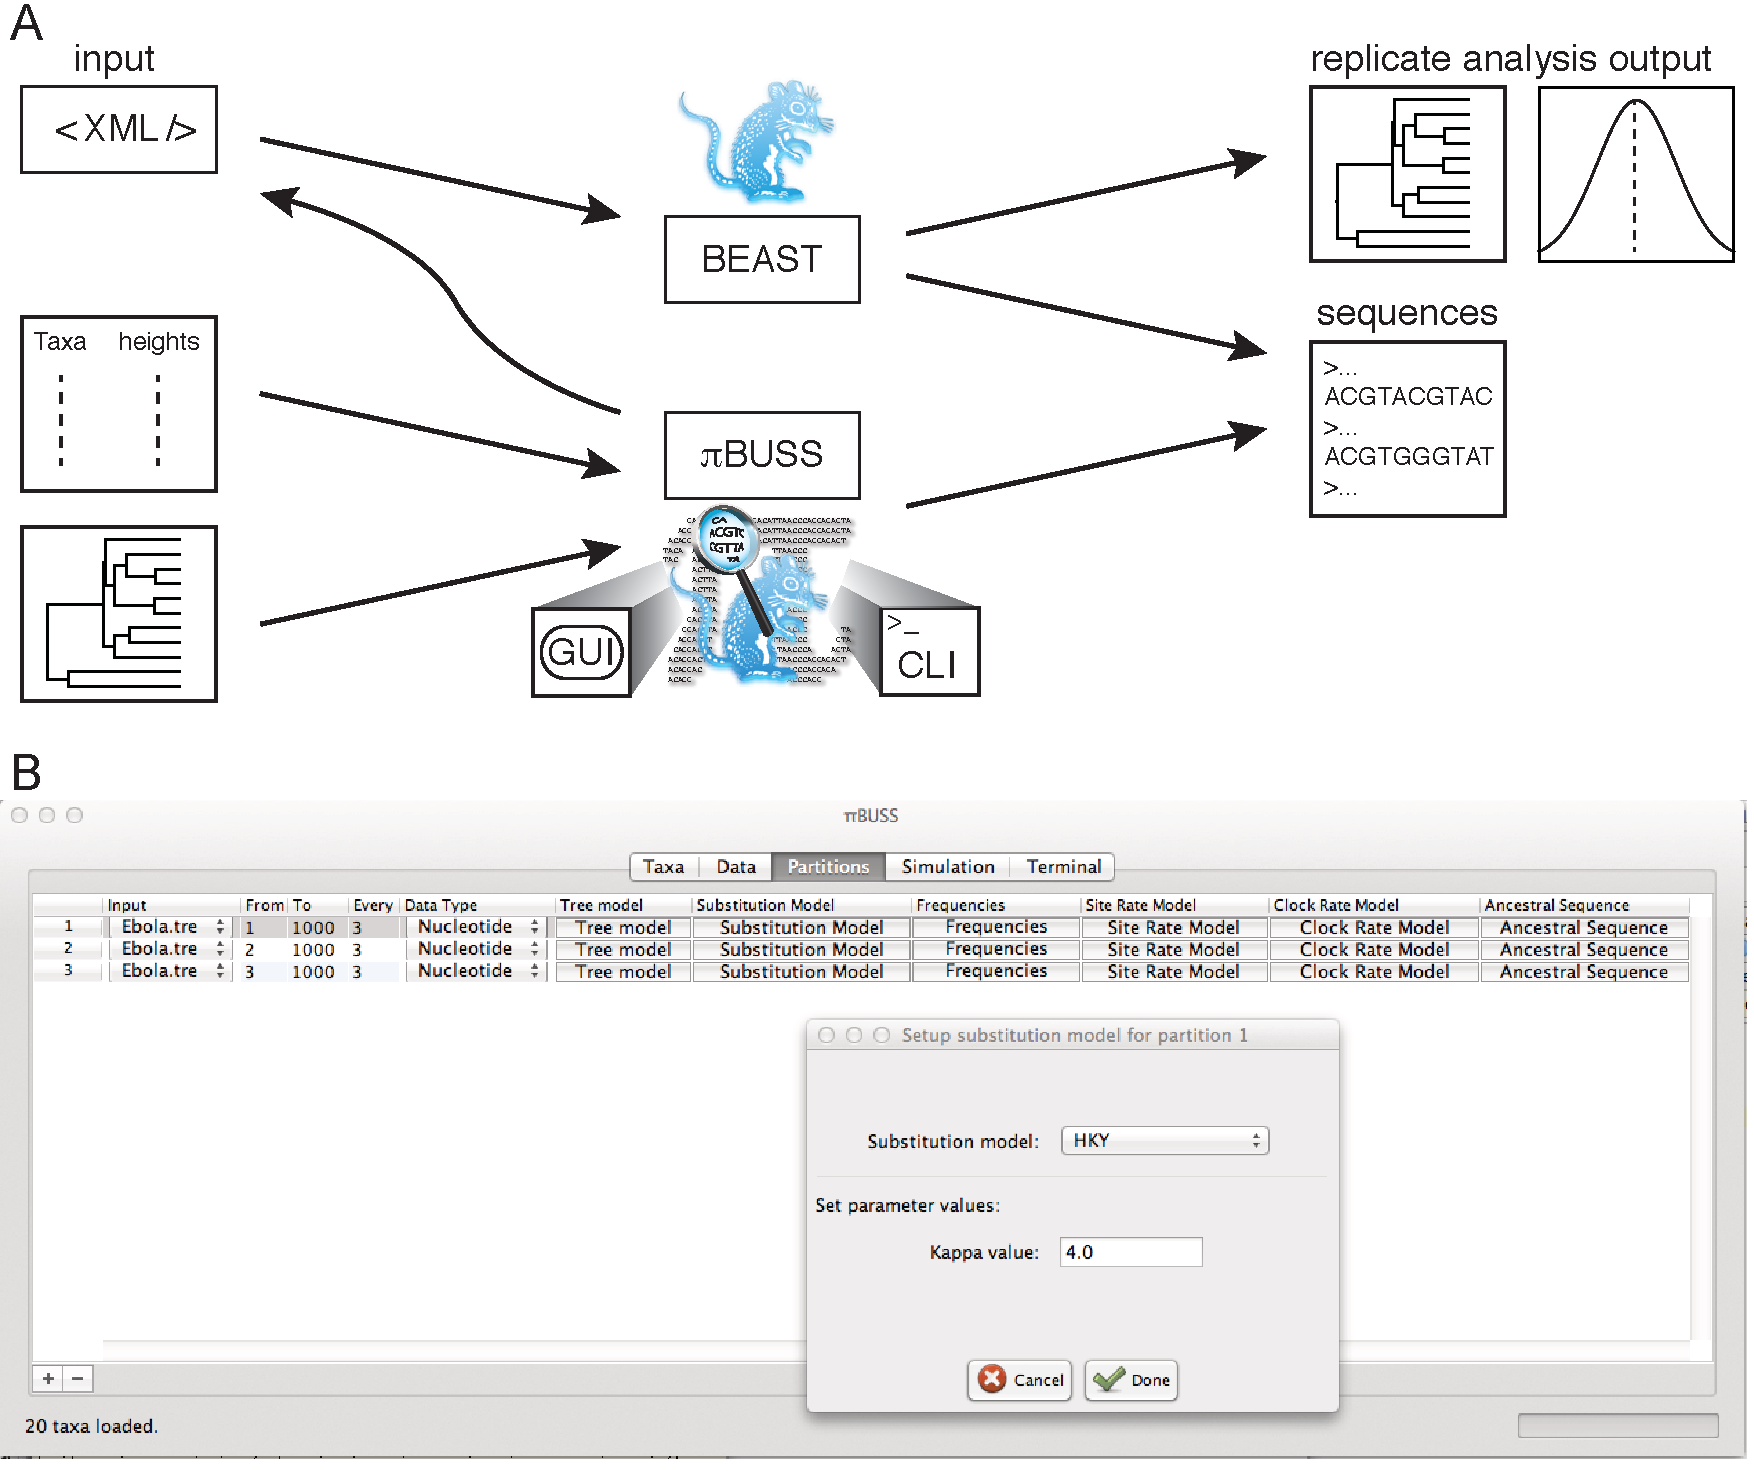
\includegraphics[scale=0.35]{schema.pdf} 
\caption{
{ \footnotesize 
{\bf Overview of the {\bussname} simulation procedures and GUI screenshot.}
A. Schematic representation of the different ways to employ the {\bussname} simulation software.
Based on an XML input file, simulations can be performed using the core implementation. %in BEAST.
BEAST can parse the specified {\bussname} instructions and generate sequence data as well as analyze the replicate data in a single run.
Using both the GUI or CLI, {\bussname} can run simulations based on an input tree or a list of taxa and their heights.
The software can also write the simulation settings to an XML file that can be then read by BEAST. 
B. The screenshot example shows the set-up of a codon position partitioned simulation in the Partitions panel of the graphical user interface.
The Hasegawa, Kishino and Yano (HKY) model is being set as the substitution model for partition 1, with a $\kappa$ (the transition-transversion bias) parameter value of $4.0$.
}% END: footnotesize 
}
\label{fig:screenshot}
\end{figure}


The core of {\bussname} consists of a recursive tree-traversal that is independent of the BEAST inference machinery. 
The algorithm simulates discrete state realizations by visiting the tree nodes in pre-order fashion, i.e., parental nodes are visited before child nodes.
When a child node is visited, {\bussname} samples its state from the conditional probabilities of changing to state $j$ given state $i$ at the parental node.
For a branch length $t$ and clock rate $r$, the finite-time transition probability matrix $\mathbf{P}\left(r\times t\right)$ is calculated through the eigen-decomposition of the infinitesimal rate matrix $\mathbf{Q}$ along that branch. 
For a review of methods to numerically approximate a matrix exponential, we refer to \cite{Moler1978}.

By sharing the set of XML parsers with BEAST, we
simplify the simultaneous development of both packages and facilitate the ability to perform joint simulation and inference analyses.

\subsection{Program input} 

The core implementation of the software can be invoked by loading an XML file with simulation settings in the BEAST software.
The simulation procedure requires a user-specified tree topology or a set of taxa with their heights (inversely proportional to their sampling time) for which a tree topology can be simulated using a coalescent model.
Setting all heights to 0 would be equivalent to contemporaneously-sampled taxa.
In {\bussname}, such a tree can be loaded in NEXUS or NEWICK format, or a taxa list can be set-up in the Data panel for subsequent coalescent simulation of the genealogy.
Creating the latter is further facilitated by the ability to load a tab-delimited file with a set of taxa and their corresponding heights.
The input tree or taxon list can also be specified through the command-line interface of {\bussname}.
 
\subsection{Program output} 

{\bussname} generates sequence output in FASTA or NEXUS format but it also supports XML output of the simulation settings. 
The XML provides a notation for the models used, it can also be used to store a record of the settings.
Similar to BEAuti for BEAST, {\bussname} can generate an xml template for editing more complex simulations, or this can be amended with BEAST analysis settings order to directly analyze the generated sequence data, which avoids writing to an intermediate file.
The tutorial hosted on {\bussname} webpage provides examples of these possibilities.

\subsection{Models of evolution} 

{\bussname} is capable of generating trees from a list of taxa using simple coalescent models, including a constant population size or exponential growth model.
The software supports simulation of nucleotide, amino acid and codon data along the simulated or user-specified phylogeny using standard substitution models.
For nucleotide data, the Hasegawa, Kishino and Yano model (HKY; \cite{Hasegawa1985}), the Tamura Nei model (TN93; \cite{Tamura1993}) and the general time-reversible model (GTR; \cite{GTR}) can be selected from a drop-down list, and more restrictive continuous-time Markov chain (CTMC) models can be specified by tailoring parameters values.  
Coding sequences can be simulated following the Goldman and Yang model of codon evolution (GY94; \cite{Goldman1994}), which is parameterized in terms of a non-synonymous and synonymous substitution rate ratio ($dN/dS$ or $\omega$) and a transition/transversion rate ratio ($\kappa$) or following the Muse and Gaut model (MG94; \cite{Muse1994}).
Several empirical amino acid substitution models are implemented, including the Dayhoff \cite{Dayhoff1978}, JTT \cite{Jones1992}, BLOSUM \cite{Henikoff1992}, WAG \cite{WAG} and LG \cite{LG} model.
Equilibrium frequencies can be specified for all substitution models as well as among-site rate heterogeneity through the widely-used discrete-gamma distribution \cite{Yang1996} and proportion of invariant sites \cite{Gu1995}. 

An important feature of {\bussname} is the ability to set up an arbitrary number of partitions for the sequence data and associate independent substitution models to them.
Such settings may reflect codon position-specific evolutionary patterns or approximate genome architecture with separate substitution patterns for coding and non-coding regions.
Partitions may also be set to evolve along different phylogenies, which could be used, for example, to investigate the impact of recombination or to assess the performance of recombination detection programs in specific cases.
Finally, partitions do not need to share the exact same taxa (e.g. reflecting differential taxon sampling), and in partitions where a particular taxon is not represented the relevant sequence will be padded with gaps. 

{\bussname} is equipped with the ability to simulate evolutionary processes on trees calibrated in time units. 
Under the strict clock assumption, this is achieved by specifying an evolutionary rate parameter that scales each branch from time units into substitution units.
{\bussname} also supports branch-specific scalers drawn independently and identically from an underlying distribution (e.g. log normal or inverse Gaussian distributions), modeling an uncorrelated relaxed clock process \cite{Drummond2006}.
Simulations do not need to accommodate an explicit temporal dimension and input trees with branch lengths in substitution units will maintain these units with the default clock rate of 1 (substitution/per site/per time unit).

The data types and models described above are available through the {\bussname} GUI or CLI, but additional data types and more complex models can be specified directly in an XML file.
This allows, for example, simulating any discrete trait, e.g. representing phylogeographic locations, under reversible and nonreversible models \cite{Lemey2009,Edwards2011}, with potentially sparse CTMC matrices \cite{Lemey2009}, as well as simulating a combination of sequence data and such traits.
As an example of available model extensions is the ability to specify different CTMC matrices over different time intervals of the evolutionary history, allowing for example to model changing selective constraints through different codon model parameterizations or seasonal migration processes for viral phylogeographic traits \citep{Bielejec2014a}.

\section{Results and Discussion}

We have developed a new simulation tool, called {\bussname}, that we consider to be a rejuvenation of Seq-Gen \citep{Rambaut1997}, with several extensions to better integrate with the BEAST inference framework.
Compared to Seq-Gen and other simulation software (Table~\ref{tab:SimSoft}), {\bussname} covers a relatively wide range of models while, similar to Mesquite, offering a cross-platform, user-friendly GUI.
{\bussname} is implemented in the Java programming language, and therefore requires a Java runtime environment, and depends on the BEAGLE library.
Although speed is unlikely to be an impeding factor in most simulation efforts, the core implementation using the BEAGLE library provides substantial increases in speed for large-scale simulations, in particular when invoking multi-core architecture to produce highly partitioned synthetic sequence data.

\afterpage{\clearpage
\begin{sidewaystable}
\centering
% {\tiny{}}%
\begin{tabular}{ccccccccccc}
\hline 
\multicolumn{8}{c}{\textbf{\tiny{Evolutionary modelling}}} & \multicolumn{3}{c}{\textbf{\tiny{Implementation}}}\tabularnewline
\textbf{\tiny{Program}} & \textbf{\tiny{Codons\footnote{\tiny{$\pi$BUSS: GY94, MG94; PhyloSim: GY94 x M0 - M4; Recodon: GY94 x M0, M1, M7, M8; NetRecodon: GY94 x M0, M1, M7, M8; Indelible: GY94 x M0 - M10; Evolver: GY94 x M0, M1, M2, M3, M7, M8; ALF: GY94 x M0, M1, M7 and M8; GenomePop: MG94}}}} & \textbf{\tiny{Amino}} & \textbf{\tiny{Indels}} & \textbf{\tiny{Partitions}} & \textbf{\tiny{Molecular}} & \textbf{\tiny{Ancestral}} & \textbf{\tiny{Coalescent}} & \textbf{\tiny{GUI}} & \textbf{\tiny{Multi-}} & \textbf{\tiny{Cross-}}\tabularnewline
 &  & \textbf{\tiny{acids}\footnote{\tiny{$\pi$BUSS: BLOSUM \cite{Henikoff1992}, CPREV \cite{cprev}, Dayhoff \cite{Dayhoff1978}, FLU \cite{FLU}, JTT \cite{Jones1992}, LG \cite{LG}, MTREV \cite{mtrev}, WAG \cite{WAG}; Seq-Gen: JTT, WAG, PAM \cite{PAM}, BLOSUM, MTREV; indel-Seq-Gen2: PAM, JTT, MTREV, CPREV; PhyloSim: CPREV, JTT, LG , MTART \cite{MTART}, MTMAM \cite{MTMAM}, MTREV24 \cite{MTREV24}, MTZOA \cite{MTZOA}, PAM, WAG; Indelible: Dayhoff, JTT, WAG, VT \cite{VT}, LG, BLOSUM, MTMAM, MTREV, MTART, CPREV, RTREV \cite{rtrev}, HIVb \cite{Nickle2007}, HIVw \cite{Nickle2007}; Evolver: Dayhoff, JTT, WAG, MTMAM, MTREV; ProteinEvolver: BLOSUM, CPREV, Dayhoff, HIVb, HIVw, JTT, Jones \cite{Jones1992}, LG, MTART, MTMAM, MTREV24, RTREV, VT, WAG; ALF: PAM,GTT,LG,WAG; SIMPROT: PAM, JTT, PMB}}} &  &  & \textbf{\tiny{clocks}} & \textbf{\tiny{sequences}} &  \textbf{\tiny{models}\footnote{\tiny{$\pi$BUSS: demography; Recodon: recombination, migration, demography; NetRecodon: recombination, migration, demography; Mesquite: speciation; ProteinEvolver: recombination, migration, demography; GenomePop: recombination, demography and migration, SIMCOAL: demography and migration}}} &  &  \textbf{\tiny{core}}  &  \textbf{\tiny{platform}
 \footnote{\tiny{PhyloSim: R package; Indelible: Executables for Windows and MacOS; ALF: Web interface; GenomePop: Executables for Windows and Linux; SIMCOAL: Executables for Windows; SIMPROT: GUI, Web interface; SIMPROT: Executables for Windows and Linux}}
 }  
 \tabularnewline
\hline 
{\tiny{$\pi$BUSS}} & {\tiny{X}} & {\tiny{X}} &  & {\tiny{X}} & {\tiny{X}} & {\tiny{X}} & {\tiny{X}} & {\tiny{X}} & {\tiny{X}} & {\tiny{X}}\tabularnewline
\gray
{\tiny{Seq-Gen \cite{Rambaut1997}}} &  & {\tiny{X}} &  & {\tiny{X}} &  &  &  &  &  & {\tiny{X}}\tabularnewline
{\tiny{indel-Seq-Gen2 \cite{Strope2009}}} &  & {\tiny{X}} & {\tiny{X}} & {\tiny{X}} &  & {\tiny{X}} &  &  &  & {\tiny{X}}\tabularnewline
\gray
{\tiny{PhyloSim \cite{Sipos2011}}} & {\tiny{X}} & {\tiny{X}} & {\tiny{X}} & {\tiny{X}} &  & {\tiny{X}} &  &   &  & {\tiny{X}}\tabularnewline
{\tiny{Recodon \cite{Arenas2007}}} & {\tiny{X}} &  &  &  &  & {\tiny{X}} & {\tiny{X}} &  & {\tiny{X}} & {\tiny{X}}\tabularnewline
\gray
{\tiny{NetRecodon \cite{Arenas2010}}} & {\tiny{X}} &  &  &  &  & {\tiny{X}} & {\tiny{X}} &  & {\tiny{X}} & {\tiny{X}}\tabularnewline
{\tiny{Indelible \cite{Fletcher2009}}} & {\tiny{X}} & {\tiny{X}} &  {\tiny{X}}  &  {\tiny{X}}  &  &   &  & {\tiny{X}}\tabularnewline
\gray
{\tiny{DAWG \cite{dawg}}} &  &  & {\tiny{X}} &  &  & {\tiny{X}} & {\tiny{X}} &  &  & {\tiny{X}}\tabularnewline
{\tiny{Mesquite \cite{mesquite}}} &  &  &  &  &  & {\tiny{X}} & {\tiny{X}} & {\tiny{X}} &  & {\tiny{X}}\tabularnewline
\gray
{\tiny{Rose \cite{Stoye1998}}} &  &  & {\tiny{X}} &  &  & {\tiny{X}} &  &  &  & \tabularnewline
{\tiny{Evolver \cite{PAML}}} & {\tiny{X}} & {\tiny{X}} &  & {\tiny{X}} &  & {\tiny{X}} &  &  &  & {\tiny{X}}\tabularnewline
\gray
{\tiny{ProteinEvolver \cite{Arenas2013}}} &  & {\tiny{X}} &  &  &  & {\tiny{X}}  & {\tiny{X}} &  & {\tiny{X}} & {\tiny{X}} \tabularnewline
{\tiny{ALF \cite{alf}}} & {\tiny{X}} & {\tiny{X}} & {\tiny{X}} & {\tiny{X}}  &  & {\tiny{X}} & {\tiny{X}}  & {\tiny{X}} &  & {\tiny{X}}\tabularnewline
\gray
{\tiny{GenomePop \cite{Carvajal2008}}} & {\tiny{X}} &  &  &  &  & {\tiny{X}} & {\tiny{X}} &  &  & {\tiny{X}}\tabularnewline
{\tiny{SIMCOAL \cite{Excoffier2000}}} &  &  &  &  &  & {\tiny{X}} & {\tiny{X}}  &  &  & {\tiny{X}}\tabularnewline
\gray
{\tiny{SIMPROT \cite{Pang2005}}} &  & {\tiny{X}} & {\tiny{X}} &  &  & {\tiny{X}} &  & {\tiny{X}} &  & {\tiny{X}}\tabularnewline
\end{tabular}
% {\tiny \par}
\caption{
{ \footnotesize 
{\bf Comparison between a selection of sequence simulation packages.} 
% We compare the availability of evolutionary modeling options and software implementation aspects of 16 sequence simulation packages. We indicate the general presence of a feature or option and provide more detail . 
}% END: footnotesize
}
\label{tab:SimSoft} 
\end{sidewaystable}
\clearpage }% END: afterpage

\subsection{Program validation}

We validate {\bussname} in several ways. 
First, we compare the expected site probabilities, as calculated using tree pruning recursion \cite{Felsenstein1981}, with the observed counts resulting from {\bussname} simulations. 
To this purpose, we calculate the probabilities for all $4^3$ possible nucleotide site patterns observed at the tips of a particular 3-taxon topology using an HKY model with a discrete gamma distribution to model rate variation among sites.
We then compare these probabilities to long-run ($n = 100,000$) site pattern frequencies simulated under this model and observe good correspondence in distribution (Pearson's $\chi^2$ test, $p = 0.42$).

We also perform simulations over larger trees and estimate substitution parameters (e.g. $\kappa$ in the HKY model) using BEAST for a large number of replicates. 
Not only do the posterior mean estimates agree very well with the simulated values, but we also find close to nominal coverage, and relatively small bias and variance (mean squared error).
These good performance measures have also recently been demonstrated for more complex substitution processes \cite{Bielejec2014a}.

\subsection{Example application}

We illustrate the use of simulating sequence data along time-calibrated phylogenies to explore the limitations of estimating old divergence times for rapidly-evolving viruses.  
Wertheim and Kosakovsky Pond \citep{Wertheim2011} examine the evolutionary history of Ebola virus from sequences sampled over the span of three decades.
Although maintaining remarkable amino acid conservation, the authors estimate nucleotide substitution rates on the order of $10^{-3}$ substitutions/per site/per year and a time to most recent common ancestor (tMRCA) of about 1,000 years ago.
These estimates suggest a strong action of purifying selection to preserve amino acid residues over longer evolutionary time scales, which may not be accommodated by standard nucleotide substitution models.
The authors demonstrate that accounting for variable selective pressure using codon models can result in substantially older origins in such cases.

Here, we explore the effect of temporally varying selection pressure throughout evolutionary history on estimates of the tMRCA using nucleotide substitution models.
In particular, we model a process that is characterized by increasingly stronger purifying selection as we go further back in to time. 
To this purpose, we set up an ``epoch model'' that specifies different GY94 codon substitution processes along the evolutionary history \citep{Bielejec2014a}, and parameterize them according to a log-linear relationship between time and $\omega$.
Specifically, we let the process transition from $\omega$ = $1.0$, $0.2$, $0.1$, $0.02$, $0.01$, $0.002$, and $0.001$ at time = $10$, $50$, $100$, $500$, $1000$ and $5000$ years in the past, respectively.
We simulate a constant population size genealogy of 50 taxa, sampled evenly during a time interval of 25 years, and simulate sequences according to the time-heterogeneous codon substitution process with a constant clock rate of $3 \times 10^{-3}$ codon substitutions/codon site/year.
We simulate 100 replicates over genealogies with varying tMRCAs, by generating topologies under different population sizes parameterized by the product of effective population size ($N_{e}$) and generation time scaled in years ($\tau$):

\begin{equation}
N_{e} \times \tau=1,\; 5,\; 10,\; 50,\; 100,\; 500,\; 1000
\label{eq:gener_times}
\end{equation}

We note that under this model, trees with tMRCAs of about 10,000 years still result in sequences with a noticeable degree of homology (resulting in a mean amino acid distance of about 0.5, which is in the same range of the mean amino acid distance for sequences representative of the primate immunodeficiency virus diversity).
Using a constant $\omega$ of 0.5 on the other hand results in fairly randomized sequences.
We subsequently analyze the replicate data using a codon position partitioned nucleotide substitution model in BEAST and plot the correspondence between simulated and estimated tMRCAs in Figure~\ref{fig:deep_root}.

\begin{figure}[h!]
\centering
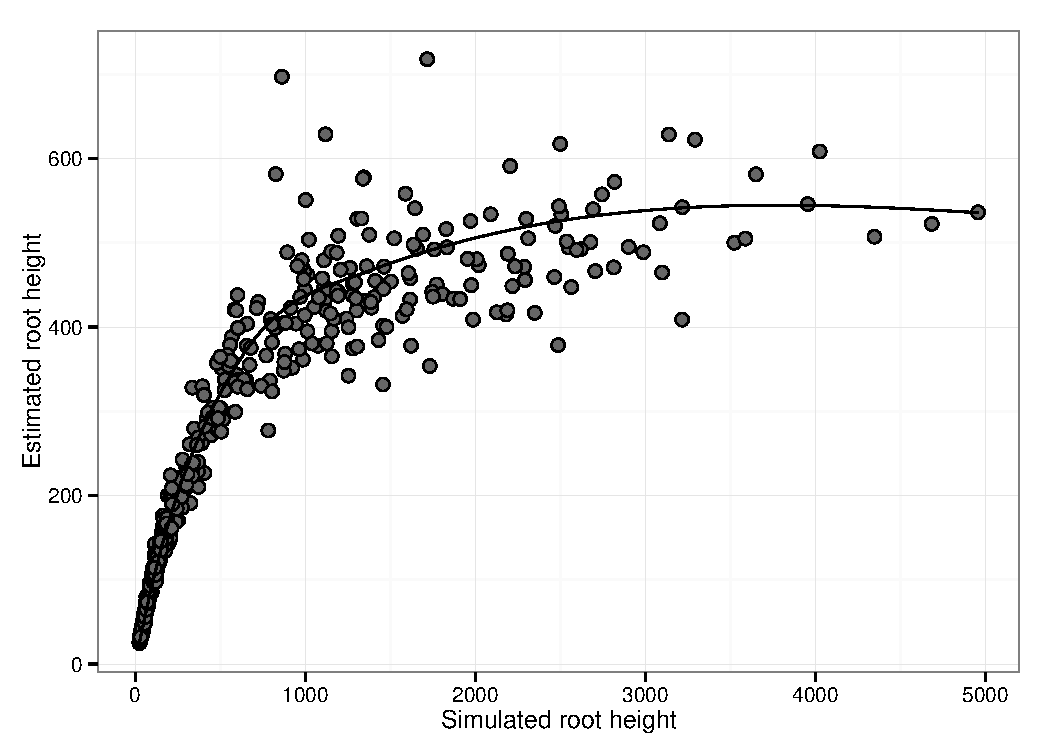
\includegraphics[scale=0.6]{deep_root} 
\caption{
{ \footnotesize
{\bf Correspondence between simulated and estimated tMRCAs when purifying selection increases back in time in simulated data sets.} 
}% END: footnotesize
}
\label{fig:deep_root}
\end{figure}

Our simulation exercise shows that a linear relationship between simulated and estimated tMRCAs only holds for 100 to 200 years in the past, and estimates quickly level off after about 1000 years in the past.
This can be explained by the unaccounted decline in amino acid substitutions and saturation of the synonymous substitutions as we go further back in time.
Although we are not claiming that evolution occurs quantitatively or even qualitatively according to the particular process we simulate under, and we ignore other confounding factors (such as potential selective constraints on non-neutral synonymous sites), this simulation does conceptualize some of the limitations to estimating ancient origins for rapidly evolving viruses that experience strong purifying selection over longer evolutionary time scales.

\section{Conclusion}

{\bussname} provides simulation procedures under many evolutionary models or combinations of models available in the BEAST framework.  
This feature facilitates the evaluation of estimator performance during the development of novel inference techniques and the generation of predictive distributions under a wide range of evolutionary scenarios that remain critical for testing competing evolutionary hypotheses.
Combinations of different evolutionary models can be accessed through a GUI or CLI, and further extensions can be specified in XML format with a syntax familiar to the BEAST user community.
Analogous to the continuing effort to support model set-up for BEAST in BEAUti, future releases of {\bussname} aim to provide simulation counterparts to the BEAST inference tools, both in terms of data types and models, while also maintaining general purposes simulation capabilities.
Interesting targets include discrete traits, which can already be simulated through XML specification, continuously-valued phenotype data \cite{Lemey2010} and indel models.
Finally, {\bussname} provides opportunities to pursue further computational efficiency through parallelization on advancing computing technology.
We therefore hope that {\bussname} will further stimulate the development of sequence and trait evolutionary models and contribute to advancement of our knowledge about evolutionary processes.




\cleardoublepage
% \chapter{Generalised Linear Models with epoch structure\label{chap:five}}%PL: I would recommend to refer to mixed-effects modeling instead of GLM, see below

\begin{remark}{Outline}
In this chapter we discuss how this work can be connected to a Bayesian implementation of Generalised Linear Models presented by \citet{Lemey2014}, in order to couple the changes of substitution rate parameters over time to the changes in external co-variates.
\end{remark}

\section{Introduction}

% In those cases an interesting solution might be to couple the unknown transition-times between epochs to external covariates for which the change-points are known, such as  the fluctuations in population size recovered by the Bayesian skyline plot model \citep{Drummond2005}.
% %GB: why the Bayesian skyline and not the skyride or skygrid? What's so specific about the skyline that it lends itself to this more than the other demographic priors?
% This approach is being investigated at the time of writing this thesis. %, yet no publishable results are currently availiable 
% % DPPs

\section{Methods}


% An interesting direction for further research is to couple epoch-specific parameters to other external covariates to inform the inference.
In the Bayesian framework this could be achieved by formulating a hierarchical phylogenetic model \citep{Edo-Matas2011}, where one put "hyperpriors" on the parameters of prior distributions to avoid over-parametrisation of the model.
%PL: thanks for referring to our GLM work for this, but the Edo-Matas2011 work already lays out all the elements we need for this: it uses hierarchical phylogenetic modeling (and you can extend the discussion on this a bit as this has some history outside of phylogenetics, and Marc basically introduced them into phylogenetics). Hierarchical modeling provides the 'random' effects, but the Edo-Matas2011 work also introduces 'fixed' effects, for which we indeed use a model averaging approach using BSVSS and quantify their support (based on the indicators) and contribution (based on the coefficients or effect sizes). So, this is essentially mixed modeling. I don't think it was referred to this as such in the Edo-Matas2011 work, so it would be nice to discuss this as such here. Note, that mixed effects modeling is also what we have used for Bram's rate variability modeling in his HIV transmission chain, and this also a direction we would like to take with your codon model developments (modeling some random branch-specific variability while testing particular selection hypotheses through fixed effects). All good points to make here, or when this part turns into a chapter, or later in the discussion!
but it also introduces fixed effects
\citet{Lemey2014} propose a model which extends the Generalized Linear Models (GLM) of \citet{Nelder1972} to the Bayesian phylogenetic framework.
Every instantaneous rate $q_{ij}$, an entry of $K \times K$ generator matrix $\mathbf{Q}$, is parametrized as a log-linear function of the set of predictors $\mathbf{X}=\left( \mathbf{x_{1}},\ldots,\mathbf{x_{P}}\right)$, where each predictor $\mathbf{x_{p}}$ is characterized by its own rate matrix such that:

\begin{equation}
log(q_{ij})=\beta_{1}\delta_{1}x_{i,j,1}+\ldots+\beta_{P}\delta_{P}x_{i,j,P}.
\label{eq:glm}
\end{equation}

Coefficients $\beta=\left(\beta_{1},\ldots,\beta_{P}\right)$ quantify the contribution of a single predictor to the overall rate, and $\left(\delta_{1},\ldots,\delta_{P}\right)$ are binary indicators that decide whether a predictor is included or excluded from the model via a Bayesian stochastic search variable selection (BSSVS) procedure \citep{Kuo1998,Lemey2009}.

For the within-host HIV evolution example analyzed in Chapter~\ref{chap:epoch}, \citet{Shankarappa1999} report both viral load and CDT4 cell count data at different time points coinciding with most sequence samplings, which could then be used as a set of potential predictors of epoch-parameter variability, and with the epoch structure %formulized 
formulated 
for that model we could infer how the linear effect of each of the covariates changes over time.
If $\mathbf{x_{p}}$ is a single predictor we can use the epoch structure to divide its time-domain into contiguous intervals.
By fitting GLM models in those intervals a piecewise effect of predictors $\mathbf{x_{p}}$ can be obtained in each epoch. 
One could begin with standard piecewise-linear changes or approximate e.g. polynomial or other complex functions of rate-change using the approach presented in Subsection~\ref{sub:nonlinear}.
%PL: of course, you will deal with this when it this turns into a chapter, but it is important to note that we would like to apply this with codon models (GY94 and MG94) to investigate the changing dynamics of selection throughout HIV infection.


%PL: I would propose the following additional discussion section, something that Nidia started to work on 
%\subsection{Combining epoch modeling with graph hierarchies for Influenza phylogeography}
%Here you can discuss that we only briefly explored the epoch application to capture seasonal influenza migration patterns in our chapter. We can make the epoch structure as complex as we want, but it of course introduces a lot of parameters to estimate, and we have already difficulties informing standard phylogeographic models with a single location state observation at the tips of the tree. One way to alleviate the over-parameterization is by sharing information across epoch parameters using hierarchical modeling (discussed above). The other one is by doing BSSVS to shrink the number of parameters, which uses 0,1-indicators to augment the CTMC state space. Cybis et al have recently suggested a hierarchical modeling approach for graphs defined by these rate indicators. So, it would be useful to examine iowa combination of epochs and hierarchical graphs these perform for this problem and what patterns they can extract, and in general, what the best way would be to model the seasonal dynamics. For example we know through the 2014 GLM work that the rates follow air traffic, so perhaps we can fix those to passenger flux between locations and only estimate when we have to turn on or off those rates using the rate indicators with their hierarchical structure. Talk to me or Nidia if you need more info


\section{Results}


\section{Discussion}


\cleardoublepage
\chapter{General discussion and future directions}

\begin{remark}{Outline}

In this concluding chapter we start with highlighting some of the ongoing work, which revolves around using a promising family of priors driven by the Dirichlet process in order to model branch and site-specific parameters of codon substitution models.

Several aspects of the presented work are then put into a wider perspective, with possible extensions discussed in more detail. 

Much of the work that constitutes this thesis resolves around relaxing the standard phylogenetic assumptions, in search of more biologically plausible models. 
In that light the work on the time-heterogenous modelling, as presented in Chapter \ref{chap:epoch}, can be viewed as an introductory step towards a broader range of models that tackle different types of time-heterogeneity.
We highlight one possible extension of the epoch model, in which time changes in a non-linear fashion.
We then discuss the possibility to infer both the time and the number of change-points, or transition times, in the epoch model specification via Dirichlet process priors discussed in the first section of this summarizing chapter. 

Another substantial portion of the work presented in this thesis is devoted towards development of flexible, easy-to-use software.
%GB: perhaps better to specify more clearly what you mean with phylogenetic and population models?
In that light we talk about the continued effort to support and extend the $\pi$BUSS simulation software \citep{Bielejec2014b}, with an ever-growing array of phylogenetic and population models.

Highly dimensional estimates that result from Bayesian inference of viral spread in both time and space require dedicated software that is capable of producing visualisations that are both visually pleasing and insightful.
We discuss the future directions that the next releases of the SPREAD software \citep{Bielejec2011} will take, ensuring that it keeps providing its users with intuitive and user-friendly interfaces as well as access to a vast bulk of possible visualisations.

Finally we talk about the challenges and opportunities that the future might bring, in the era of the so-called ``genomics plenty'', where vast amount of molecular sequences can be sequenced fast and cheaply.
\end{remark}

%%%%%%%%%%%%%%%%%%%%%%%%%%%%%%%%%%%
%---DPP PRIORS FOR CODON MODELS---%
%%%%%%%%%%%%%%%%%%%%%%%%%%%%%%%%%%%
\section{Heterogenous models of codon evolution\label{sub:dpp}}

\subsection{Introduction}

The first computationally tractable models of codon substitution were independently proposed by \cite{Muse1994} and \cite{Goldman1994} and published in the same issue of Molecular Biology and Evolution (MBE).
For codon models the non-stop codon triplet $n_{1}n_{2}n_{3}$ is considered the smallest unit of evolution.
There are $4^3$ possible triplets minus three stop codons, resulting in a state space size of $61$ codons.
The standard assumption of independence is used, i.e. the substitutions at these three codon positions occur independently, and only a single change per triplet can occur at a given time. 
%GB: explain in more detail, i.e. more than 1 change is possible in subsequent infinitesimal time intervals
%GB: are there no codon models that allow for multiple substitution per time unit (I thought I recently read something like that ... will look it up and send e-mail)
Proteins are coded by a set of 20 amino acids, with each amino acid being coded by a codon triplet. 
Because there are 61 non-stop codons, inevitably some amino acids will be redundantly coded by more than 1 codon.
A substitution which does not change the encoding amino-acid is called a synonymous substitution, as it most likely leaves the protein function unchanged.
Conversely non-synonymous substitutions are more likely to affect the fitness of a particular organism.

Selective pressure is the main force behind molecular evolution.
Understanding and inferring the selective pressure is one of the central goals of molecular virology, see for example \citet{Bielejec2014a}.
That is why most of the codon substitution models are parameterized in terms of the rate of non-synonymous (denoted by convention $\beta$) and synonymous ($\alpha$ by convention) substitutions.
Their ratio $\omega=\beta / \alpha$ is a standard measure of the selective pressure \citep{ThePhylogeneticHandbook}, which is sometimes also denoted $\omega = dN/dS$.
Prevalence of synonymous substitutions over non-synonymous ones leads to a \emph{purifying (negative)} selection, and corresponds to the ratio $\omega <1$.
If non-synonymous substitutions accumulate at a faster rate than the synonymous substitutions this is coined \emph{positive selection}, improving the fitness of the particular organism.
$\omega\approx 1$ signifies neutral evolution.

There are several advantages in using codon models over nucleotide-based substitution models.
Not all DNA positions evolve at the same rate, with non-synonymous substitutions occurring more frequently then synonymous substitutions.
Although this problem can be mitigated to some extent by using codon-positioned nucleotide substitution models, the fast evolving positions and the state space limited to 4 character alphabet still can lead to biased estimates over long evolutionary distances, as portrayed in the previous Chapter~\ref{chap:pibuss}.

% GY style models
The model proposed by \cite{Goldman1994} is characterized by a substitution rate matrix with following entries:

\footnotesize{
\begin{equation}
q_{ij}^{GY94}=\begin{cases}
\pi_{j} & \text{if \ensuremath{i\rightarrow j} is a synonymous transversion}\\
\kappa\cdot\pi_{j} & \text{if \ensuremath{i\rightarrow j} is a synonymous transition}\\
\omega\cdot\pi_{j} & \text{if \ensuremath{i\rightarrow j} is a non-synonymous transversion}\\
\omega\cdot\kappa\cdot\pi_{j} & \text{if \ensuremath{i\rightarrow j} is a non-synonymous transversion}\\
0 & \text{otherwise}
\end{cases},
\label{eq:gy94}
\end{equation}
} % END: size

\noindent
where the parameter $\kappa$ denotes the transition/transversion ratio, parameter $\omega$ denotes the non-synonymous/synonymous
rate ratio and $\pi_j$ denotes the equilibrium frequency of codon triplet $j$.
The parameters $\kappa$ and $\pi_j$ can be thought of as controlling the CTMC process at the DNA level, while the $\omega$ parameter characterizes the selection on non-synonymous substitutions.
For the GY94 model the synonymous evolutionary rate is fixed to be 1, i.e. $\omega=\beta$.

Different flavours of the GY94 model differ in the composition of the equilibrium codon frequency parameter $\pi_{j}$.
One approach is to model the codon frequencies as each having the same long-time frequency of appearing. 
Such model is referred to as the GY94-Fequal.

In the GY94-F$1\times4$ model codon frequencies are calculated from the four nucleotide frequencies, with frequencies being pulled from all three codon positions, i.e. $\pi_{n_{1}}=\pi_{n_{2}}=\pi_{n_{3}}$ for all four nucleotides,.
This model leads to 3 free parameters that need to be estimated from the data. 
%GB: they're often not estimated during the MCMC run, but empirical values are used.
%GB: how are these 'nucleotide frequencies' then used to calculate the 'codon frequencies' ?
If the frequencies are parameterized according to three sets of nucleotide frequencies for the three codon positions, resulting in nine free parameters, the model is called the GY94-F$3\times4$.
Finally in the GY94-F61 model every codon triplet has it's own frequency parameter, with all parameters summing to one, resulting in 60 free parameters that need to be estimated.

The GY94-F61 model has been suggested as important in letting the model explain the data without constricting assumptions.
\citet{Rodrigue2008} however argue that the model has no interpretation on the nucleotide level as well as confounds other effects inducing uneven codon stationary probabilities.
The authors criticize the GY94-F$3\times4$ setup as superficial, pointing that the periodic pattern along the nucleotide sequence positions represents the coding structure of the sequence but not the processes that shape the evolution.

% MG style models
The Markov generator matrix for MG94 style models \citep{Muse1994} is given by:

{\tiny{
\begin{equation}
q_{ij}^{MG94}=\begin{cases}
\alpha\cdot\kappa\cdot\pi_{n}^{p} & i\rightarrow j\text{ is a synonymous transition from nucleotide \textit{m} to \ensuremath{n} at codon position \ensuremath{p}}\\
\alpha\cdot\pi_{n}^{p} & \text{synonymous transversion from \ensuremath{m} to \ensuremath{n} at position \ensuremath{p}}\\
\beta\cdot\kappa\cdot\pi_{n}^{p} & \text{non-synonymous transition from \ensuremath{m} to \ensuremath{n} at position \ensuremath{p}}\\
\beta\cdot\pi_{n}^{p} & \text{non-synonymous transversion from \ensuremath{m} to \ensuremath{n} at position \ensuremath{p}}\\
0 & \text{otherwise}
% \alpha\cdot\kappa\cdot\pi_{n}^{p} & i\rightarrow j\text{ is a synonymous transition from nucleotide \textit{m} to \ensuremath{n} at codon position \ensuremath{p}.}\\
% \alpha\cdot\pi_{n}^{p} & i\rightarrow j\text{ is a synonymous transversion from nucleotide \ensuremath{m} to \ensuremath{n} at codon position \ensuremath{p}.}\\
% \beta\cdot\kappa\cdot\pi_{n}^{p} & i\rightarrow j\text{ is a non-synonymous transition from nucleotide \ensuremath{m} to \ensuremath{n} at codon position \ensuremath{p}.}\\
% \beta\cdot\pi_{n}^{p} & i\rightarrow j\text{ is a non-synonymous transversion from nucleotide \ensuremath{m} to \ensuremath{n} at codon position \ensuremath{p}.}\\
% 0 & \text{otherwise.}
\end{cases},
\label{eq:mg94}
\end{equation}
} % END: size
}

There are two main differences to be noted with respect to the GY94 style codon models.
First, the model is parameterized in terms of both the non-synonymous ($\beta$) and synonymous ($\alpha$) rates, meaning that a change in the ratio may be due to alteration of the rate of non-synonymous or synonymous substitutions, or both.
Second, the model estimates the frequencies of the target nucleotide $\pi_{n}^{p}$ rather than of the target codon triplet $\pi_{j}$, as in the GY94 model.
As before the MG94 model can be used with frequencies specified as a single (MG94-F$1\times4$) or three (MG94-F$3\times4$) vectors with 4 dimensions.
For the remainder of this chapter we will focus our estimation on the MG94 parameterization, mostly because the parameterization in terms of both the synonymous and non-synonymous substitution rates offers interesting opportunities for disentangling the patterns of correlation between the two.

% first talk about across site variation
%GB: when you say constant, do you mean homogeneous?
Molecular phylogenetic analyses using codon models are typically restricted to fitting a single model, with constant parameterization across data, i.e. sites of the alignment.
However there is no biological reason to assume that all the sites are under the same selection regime.
\cite{NY98} point towards the fact that for most real world data sets, of which we know that they evolved under positive selection pressure only a handful of sites actually contributed towards the non-synonymous to synonymous rates ratio >1.
%GB: replace constant with homogeneous?
Therefore, applying constant model to the data, without accounting for across-data heterogeneity, biases the estimates of $dN/dS$ ratio towards lower values.
In some cases this might lead to a failure in detecting positive selection even if it's actually present in the data.  
In that respect \cite{NY98} propose two models in the GY94 context, with a fixed number of categories to which a particular site can belong.
Their \emph{neutral model} assumes a category for sites where the non-synonymous mutations are neutral ($\omega_1=1$) and a category for sites which are conserved ($\omega_2=0$).
Their \emph{positive selection model} adds an extra category of positively selected sites ($\omega_3>1$).
\cite{Goode2008} employ this setup and further extend it by allowing for a change in $\omega$ parameter value at some specified time between the most-recent common ancestor and the most recent sampling time.

These models, although undeniably a step in the right direction, still make strong assumptions, among which partitioning sites into a fixed number of rate classes and estimating the rate for each class separately is probably the most restrictive one.
Ideally, the model should let the data decide how many rate classes there are, and what the site-specific values are.

A first modelling approach that comes to mind is to fit a different rate to each site in the alignment \citep{Nielsen1997}.
Although this approach might seem naive at first, it bears a valuable property in that no explicit assumption in the distribution of rates across sites is being made.
However other negative factors still persist, precluding such a class of methods from being generally applicable.
The main problem is that, particularly for long sequences, many parameters need to be estimated, increasing the computational costs.
In case of shorter sequences such a method may overfit the data, leading to a significant loss of statistical power and biased estimates.
Another approach treats site-specific rates as independent draws from some common distribution, e.g. a gamma distribution \citep{Yang1993} or inverse Gaussian probability distribution \citep{Waddell1997}, sometimes with a proportion of sites allowed to remain invariable \citep{Gu1995}.
This approach allows to model the rate variation with relatively few parameters, as well as provides pooled estimates of the distribution parameters, which can in turn be compared across different data-sets.  
In many scenarios though a single parametric distribution proves too naive of an approach to capture complex patterns of rate evolution \citep{Pond2005a}.
\cite{Yang2000} proposed to model among-site substitution rate variation in codon models by employing a mixture of different distributions.
Although mathematically possible, this proved computationally too expensive to fit mixtures of continuous distributions for the parameters of interest and the authors resort to fitting discrete approximations.
Although these constraints are being actively stretched \citep{Suchard2009,Ayres2012}, averaging over a large array of distributions remains computationally intensive. 
\citet{Pond2005a} propose a simple, yet flexible model of rate variation with an integrative method to reliably estimate the fluctuating parameters.
This method proceeds by partitioning the rate distribution into a countable number of intervals, with each interval represented by some statistic.
%GB: explain this beta model thingy
Then a beta model is used to decide what intervals the underlying rate distribution is partitioned into and calculate corresponding rate class values.
This is perhaps the most flexible approach for evaluating site-specific rate variation to date, that provides a good fit to data with only a few extra parameters.

\cite{Heath2012} introduces a model which relaxes the assumption of a strict molecular clock in a way that is alternative to the Random Local Clock models (\cite{Drummond2010}, see Subsection~\ref{sub:clocks}), which proceed by clustering branches on a tree which share the same rate.
In the approach proposed by \cite{Heath2012} both the number of the rate classes, as well as their placement are modeled using a Dirichlet process prior (DPP, \cite{Ferguson1973}). % which treats them as random variables.
Here we propose an approach which is similar in spirit to \cite{Heath2012}, although our interest lies not in modelling overall branch rates, but in modelling across-lineage heterogeneity of the parameters of codon substitution models, such as the synonymous and non-synonymous substitution rates.

Both the number and the clustering of the lineage-specific parameters are treated as random, and are controlled by a Dirichlet Process Prior.
A DPP is a "distribution over distributions" and induces clusterings with a varying number of components that can grow or shrink depending on the data and a concentration parameter.
It is thus often used as a prior over possible clusterings where the exact number and population of distinct clusters is not known beforehand.
We require no structure to be enforced on the clustering of the branches, and allow the data to drive the model in a descriptive fashion. 
Our only requirement is the prior specification of the concentration parameter of DPP, controlling whether a model prefers less clusters with many occupants or more less densely populated ones. 
By implementing our model as part of BEAST's Bayesian inference framework we allow for a hyperprior to be put on this parameter to average over all of its possible values. 
This approach avoids overparameterisation and computational overhead by achieving data-driven balance between simplicity and complexity of the model.
We use Markov chain Monte Carlo (MCMC) techniques, in which a chain with a memoryless property is constructed to draw samples from the posterior.
Although we focus our efforts on estimating the patterns of variation in codon substitution models our implementation is generally applicable to any parameters that exhibit across-data or across-time heterogeneity .
Below we describe the main aspects of the model.

\subsection{Methods}

We use a Dirichlet process prior (DPP) to model branch-specific codon parameters.
In real-world applications not every branch in the tree would display the same type of evolutonary behaviour, therefore it would be natural to expect some degree of clustering between them.
Suppose one is interested in a branch-specific parameter $\theta_{i}, i=1,\ldots,N$, where $N=2n-1$ is the number of branches in a tree with $n$ taxa. 
This parameter might be multi-dimensional, yet for simplicity our notation will be limited to the univariate case.
We expect \emph{a priori} that $K\ll N$, where $K$ denotes the number of unique clusters of branches.
All of the branch-specific parameters have the same distribution $B$:

\begin{equation}
\forall i=1,\ldots,N: \theta_{i}\sim B(\mu_{z_{i}}),
\label{eq:dpp1}
\end{equation}

\noindent
where we will use $\mathbf{z}$ to denote the vector of branch category assignments.
Each branch receives a category $z_{i},\; i\in\left\{ 1,\ldots K\right\}$, where $K\in\left\{ 1,\ldots,N\right\}$ denotes the a number of branch categories.
As an example let us consider a topology $\mathbf{F}$ with $N=3$ branches and a fixed number of categories $K=2$.
One possible realization of the vector of assignments would then be:

$$\mathbf{z}=\left(z(1)=1,\; z(2)=1,\; z(3)=2\right),$$ 

\noindent
meaning that branches one and two belong to the same category 1, and that the third branch belongs to the category 2.
Let us denote the uniquely realized branch-specific parameter values by $\hat{\theta_{j}}, j=1,\ldots,K$.
%GB: what do you mean when you say 'mechanistic' ? Do you mean 'deterministic' ?
A mechanistic function $f$ keeps track of the mapping between the branches and unique realizations $\hat{\theta_{j}}$:

\begin{equation}
\mu_{z_{1}},\ldots,\mu_{z_{N}}=f\left(\hat{\theta}_{1},\ldots,\hat{\theta}_{K},z_{1},\ldots z_{N}\right).
\label{eq:dpp2}
\end{equation}

\noindent
The idea behind using DP priors is to set up a kernel distribution with probability distribution function $P_{0}$ from which unique branch-specific candidate values $\hat{\theta_{j}}$ are drawn:

\begin{equation}
\forall i=1,\ldots,N\;\hat{\theta_{j}}\sim P_{0}\left(\mu\right).
\label{eq:dpp3}
\end{equation}

\noindent
Clustering indicators for each branch are sampled according to a Dirichlet process with intensity $\gamma$:

\begin{equation}
z_{1},\ldots,z_{N}\sim DP(\gamma).
\label{eq:dpp4}
\end{equation}

\noindent
By defining hyper-priors for the parameters of the kernel distribution and a concentration parameter of the DP, or alternatively fixing them to specific values, we complete the specification of the DPP:

\begin{equation}
\begin{array}{c}
\mu\sim P_{1}(\ldots)\\
\gamma\sim P_{2}(\ldots)
\end{array}.
\label{eq:dpp5}
\end{equation}

% One of them is to consider the branch-specific values as coming from a mixture of distributions
There are several possible implementations of the Dirichlet process for drawing the cluster indicators as defined in Equation \ref{eq:dpp4}. 
One of them is the so-called "stick-breaking" construction \citep{Sethuraman94}.
The draws from a DP are composed of a weighted sum of point masses $P$, summing up to 1 and giving rise to a discrete distribution.
The algorithm to generate a single draw from DP is given in Listing \ref{alg:stickBreaking}.

\begin{algorithm}[H]
\begin{center}
\begin{algorithmic}[1]
% \footnotesize{
%
\State $remainingLength \gets 1.0$;
%
\For{$\left( \text{int } j=0; \; j<K; \; j++\right)$}
%
\State $r\sim Beta\left(1,\gamma\right)$;
%
\State $P\left[j\right]=r \cdot remainingLength$;
%
\State $remainingLength=\left(1-r\right) \cdot remainingLength$;
%
\EndFor \\
%
 \textbf{return} $P$;
% }
\end{algorithmic}
\end{center}
\caption{ 
{ \footnotesize 
{\bf Constructing the Dirichlet process by stick breaking.} 
}% END: footnotesize
}
\label{alg:stickBreaking}
\end{algorithm}

Colloquially we can describe it as follows: we start with a stick of length 1 and break it randomly at point $r_{1}$ chosen by drawing one value from $\text{Beta}(1, \gamma)$ and assign $p_{1}$ to the length of the part of the stick that we just broke off.
We then recursively break other portions of the stick to obtain $p_{2}, p_{3}, \ldots$ and so forth, each time setting:

\begin{equation}
p_{i}=r_{i}\cdot\underset{j}{\overset{i-1}{\prod}}\left(1-r_{j}\right).
\label{eq:sticks}
\end{equation}

\noindent
Parameter $\gamma$ controls the clustering behaviour of the process.
Smaller values will lead to fewer, yet more populated categories; larger values will result in more categories being occupied by less branches.

Under our DPP model both the number of categories $K$ and category assignments $z_{i}$ are random variables, controlled by a DPP with a concentration parameter $\gamma$ and a base distribution given by $P_{0}$.
The complete likelihood of the model can be written down as:

\begin{equation}
L(\mathbf{z},K|\gamma,N,\hat{\theta_{1}},\ldots,\hat{\theta_{K}})=\gamma^{K}\cdot\frac{\underset{j=1}{\overset{K}{\prod}}\left(\eta_{j}-1\right)!}{\underset{i=1}{\overset{N}{\prod}}\left(\gamma+i-1\right)}\cdot\underset{j=1}{\overset{K}{\prod}}P_{0}\left(\hat{\theta_{j}}\right)^{\eta_{j}},
\label{eq:dppLike} 
\end{equation} 

\noindent 
where $\eta_{k}$ denotes the number of sites assigned to category $k$.
%GB: do you want to talk about the increased computational demands of codon models? and how this can be alleviated by using BEAGLE on GPUs?
%GB: do you w  ant to show a figure that explains the redundancy of the genetic code?

\subsection{Summary}
% TODO: call it `Summary & Preliminary Results', show some numericla results + plots from tests on the Galaxy data

This model is currently being  implemented in the BEAST software package.
This pending implementation is currently being tested against an implementation in the JAGS software \citep{Plummer2003}, and we are using a numerical example to compare the results.

%%%%%%%%%%%%%%%%%%%%%%%%%%%%%%
%---EPOCH MODEL EXTENSIONS---%
%%%%%%%%%%%%%%%%%%%%%%%%%%%%%%
\section{Extending the Epoch model}

In Chapter \ref{chap:epoch} we presented a time-heterogeneous substitution model, for which the different types of substitution rates %of evolution
remain constant across all lineages in any given epoch, but vary between those epochs.
We have demonstrated the validity of the method using simulations, and its applicability to empirical HIV and Influenza data sets.
We have stressed that by implementing the model as part of Bayesian framework we are able to incorporate uncertainty in the tree reconstruction into our analysis, and thus avoid the need to fix the tree topology or any other evolutionary parameters.

\subsection{Approximating non-linear functions of rate change in time\label{sub:nonlinear}}

For some classes of problems the substitution rates might not vary linearly, at the defined change-points, but rather as some arbitrarily complex function of time. 
Such functions may be difficult, or computationally demanding, to fit exactly and the epoch model may offer an approximate solution to this types of problems.
Let us consider an interval $\left[0,T\right]$ and let the elements of the substitution rate matrix $\mathbf{Q}$ vary independently as an integrable function of time, such that $\mathbf{Q}=\mathbf{Q}(t),\; t\in\left[0,T\right]$. 
Finite-time transition probabilities can be then calculated as: 

\begin{equation}
\ensuremath{\mathbf{P}}(r,T)=exp\left(r\int_{0}^{T}\mathbf{Q}(t)dt\right).\label{eq:rodrigo}
\end{equation}

\noindent
\citet{Rodrigo2008} propose a numerical approximation to $\int_{0}^{T}\mathbf{Q}(t)dt$. 
By taking points $t_{0,}t_{1},\ldots t_{n}\in[0,T]$ such that $0=t_{0}<t_{1}<\ldots<t_{n}=T$ and dividing the interval $\left[0,T\right]$ into sub-intervals $\left[t_{i-1},t_{i}\right],\; i=1,\ldots n$ of length $\triangle t_{i}=t_{i}-t_{i-1}$ we have that:   

\begin{equation}
\int_{0}^{T}\mathbf{Q}(t)dt\approx\underset{i=0}{\overset{n}{\sum}}\mathbf{Q}(t_{i}^{*})\cdot\triangle t_{i},\; t_{i}^{*}\in[t_{i-1},t_{i}].\label{eq:approx}
\end{equation}

\noindent
From Equations~(\ref{eq:rodrigo}) and (\ref{eq:approx}), by the definition of the Riemannian integral we have that $\mathbf{P}(r,T)=\underset{n\rightarrow\infty}{lim}\underset{i=0}{\overset{n}{\prod}}\text{exp}\left(r\mathbf{Q}(t_{i}^{*})\cdot\triangle t_{i}\right)$, given that rate matrices $\mathbf{Q}(t_{i}^{*})$ commute 
and are closed with respect to the matrix multiplication.
\citet{Sumner2012} formalize the problem of multiplicative closure of the Markov models. 
Given those regularity conditions, we can perform a numerical approximation of any function of rate change by using the epoch time-discretization, and by partitioning the time interval into a fine grid of intervals.
Extending our Bayesian epoch model implementation to accommodate complex rate change functions could be the focus of future work when confronted with a problem that would benefit from such an approach.

\subsection{Evaluating number and placement of change-points in time}

Both problems presented in Chapter~\ref{chap:epoch}, i.e. HIV within-host evolution before and after progression time and seasonal influenza migration represent hypotheses that condition on a particular  number and placement the transition times.
There might however be a class of problems for which those change points are not known and need to be estimated.
% it remains interesting to investigate possible extensions that estimate the number and position of change points.
A first approach that comes to mind is to introduce priors on the number and locations of the transition times and integrate over all their possible values using the standard MCMC framework.
This straight-forward approach will however inflate the variance of the epoch-specific parameters and for some problems, e.g. viral diffusion between discretely sampled geographical locations where there is only one observation per taxon, the sparseness of data might be a factor impeding any accurate inference.

In Subsection \ref{sub:dpp} we talk about an interesting class of non-parametric prior distributions, the so called Dirichlet Process Priors (DPP). 
Although we mainly pursue the inference of lineage-specific parameters of codon models, it is interesting to note that the same class of priors could be used to infer the number and placement of transition-times of the epoch model.
At the time of writing this chapter we are testing these possibilities, yet exactly how accurate the inference of the transition times can be, and how we can quantify the predictive value of those covariates remains an open question for future studies.

%%%%%%%%%%%%%%
%---SPREAD---%
%%%%%%%%%%%%%%
\section{Future prospects for visualizing viral diffusion}

% Genetic and phenotypic data become useful only when we apply methods deriving insights from it, and these methods encompass statistical inference as well as visualization of its results. Visualizing estimates provides an efficient way to communicate results to the scientific community and beyond. Bayesian evolutionary inference, however, generates \textbf{high-dimensional} estimates, e.g. ancestral reconstructions of (multiple) traits on a posterior distribution of trees. When multidimensionality complicates the visualization task, dynamic, interactive visualizations may offer an attractive solution. In our case, the time scale of the evolutionary histories represents a natural dimension to explore for dynamic interactions. Interactivity can also encourage engagement and may lead to a better understanding and even appreciation of the statistical inference procedure itself. 

\paragraph{}
In Section~\ref{sub:clocks} we discussed how past evolutionary events can be estimated in real time units by using molecular clock models and either calibrating events or, in case of MEPs, samples obtained at various points in time.
A natural representation of this temporal dimension is to animate the geophylogeny as it unfolds through time and space.
The visualisation of spatiotemporal history, with the possibility to dynamically examine how the diffusion process unfolds, has been the main motivation for the development of SPREAD \citep{Bielejec2011}, presented in Chapter~\ref{chap:spread}.
SPREAD allows for visualising animated geophylogenies in an automated manner, by producing it's output in time-annotated Keyhole Markup Language (KML), an ISO standard geographic markup language managed by the Open Geospatial Consortium that is read and written by most spatial software. 
KML encoding allows for manipulating virtually all aspects of mapping, colour and line thicknesses, time animation, height and placement, projection used, labelling and many more.
SPREADs GUI gives user a control over fine-tuning these parameters and the output can be used in virtual globe software like Google Earth (\url{http://www.google.com/earth/}) or high-end GIS software like ArcGIS, Cartographica.
Here we take the opportunity to discuss the design and future directions of SPREAD in more details.

\subsection{Past and current efforts in visualising phylogeography}

Geophylogenies, or more generally geo-trees are spatially referenced phylogenies, for which taxa exist in a real space and can be displayed as cartographic elements within a map \citep{Kidd2010}.   
Possibly the first diagram like that, depicting evolutionary tree over geographical map is the famous \textit{Hypothetical Sketch of the Monophyletic Origin and the Extension of the 12 Races of Man from Lemuria over the Earth} shown in \cite{Haeckel1876} (see Figure~\ref{fig:lemuria})

\begin{figure}[H]
\centering
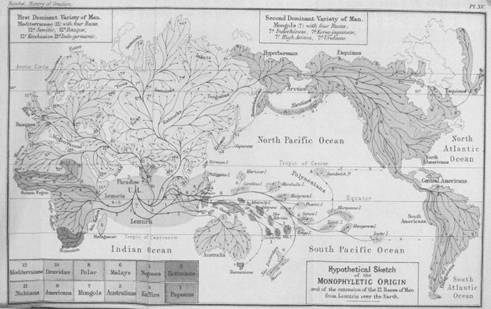
\includegraphics[scale=0.25]{lemuria}
\caption{
{ \footnotesize 
{\bf Hypothetical Sketch of the Monophyletic Origin and the Extension of the 12 Races of Man from Lemuria over the Earth.} 
} % END: footnotesize
}
\label{fig:lemuria}
\end{figure}

Ernst Haeckel, a XIX century darwinist entertained the idea that the abscence of missing fossil links in human evolution could be explained by existence of \textit{Lemuria}, a sunken land.  
The phylogentic visualisation has surpassed the, entirely discredited, work itself.

% other tools
The joint study of diffusion processes happening in geographical coordinates along with the patterns of genomic ancestry is known as phylogeography.
Summarising the findings in a clear and concise way, that can then be presented to a wider audience, is as important of a step as the statistical analysis itself \citep{Hadley2010}.
This is especially true for complex patterns of biogeographic processes, where visualisation is the key for understanding them. 
Recently great research effort has been made to visulize the phylogenetic relationships between organisms and samples in relation to their geographic distribution. 

\paragraph{}
In the first approach geographic pattern is displayed as an annotation on the tree, with branches labelled according to the names of places in which their tips are observed.
This can be carried out by hand for example in FigTree (\url{http://tree.bio.ed.ac.uk/software/figtree/}).
More advanced annotations can be achieved in iTOL \citep{itol}, which is capable of displaying charts on the internal or external branches, displaying prevalence of any kind of data, including discrete geographic locations and scaled to reflect the size of it.
This approach is most appropriate when the geographic complexity is low, as it simplifies the spatial context to text or symbolic representation, prioritising the ancestral relationship rather over the diffusion in actual geographical coordinates.

\paragraph{}
GenGis software (Figure~\ref{fig:tanglemaps}), presented by \cite{Parks2009} can, among other, generate visualisation which are an example of so-called tangle-maps.
Tangle-maps are visualisations which combine cartographic maps with images of trees.

\begin{figure}[H]
\centering
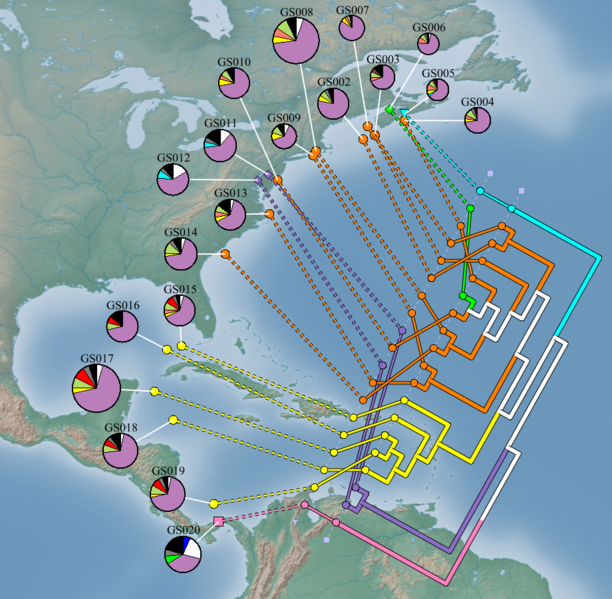
\includegraphics[scale=0.3]{tanglemaps}
\caption{
{ \footnotesize 
{\bf Tangle-map of the biodiveristy of 19 marine metagenomes.} 
Figure is plotted using GenGis (\url{http://kiwi.cs.dal.ca/GenGIS/Main_Page}).
} % END: footnotesize
}
\label{fig:tanglemaps}
\end{figure}

Although in tangle-maps the tree and the map may are visually linked through the use of graphic lines, the tree is merely overlayed on the map, rather than projected onto the geographical coordinates.

% how we do it
\paragraph{}
Model-based approaches to phylogenetic reconstruction, such as ancestral state reconstruction (see Subsection~\ref{sub:phylogeo}) provide estimates for phylogeographic relationships, but also the uncertainty in those estimates, which is crucial for hypothesis testing.
Appropriately accommodating statistical uncertainty into visualisations is a major challenge.
In BEAST and other software capable of phylogeographical reconstruction the location data can be modeled either as finite and countable (discrete) states or bivariate (longitude and latitude) realizations in continuous space.
This choice is mainly dependent on the sampling scheme of the data.
Different representations of uncertainty result from each approach.
In the continuous case when bicariate coordinates are inferred for the internal nodes using a Brownian motion model, the geographic uncertainty is expressed as confidence envelopes or credible contours for each internal node.
This can be seen in Figure~\ref{fig:cont}, where a 3D-geophylogeny with credible contours for each internal node projected on the surface in the Google Earth.

\begin{figure}[H]
\centering
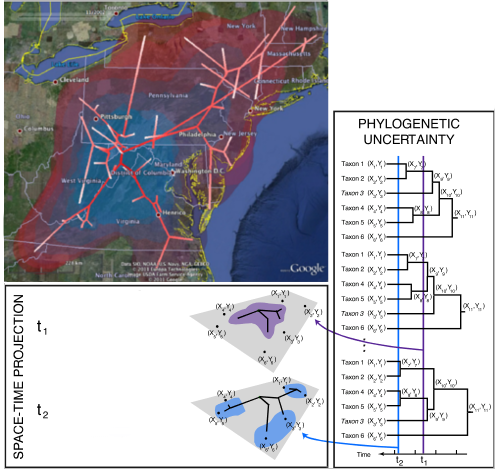
\includegraphics[scale=0.6]{continuous}
\caption{
{ \footnotesize 
{\bf Visualising geography uncertainty and phylogenetic tree uncertainty.} 
Bottom facets explain the concept of time-slicing, upper facet presents a resulting animation.
} % END: footnotesize
}
\label{fig:cont}
\end{figure}

Two time slices are shown as an example for the continuous diffusion through time. 
An example tree is mapped in continuous space, based on average bivariate coordinates for the internal nodes. 
The uncertainty at any time-slice is depicted using credible contours, obtained from slicing the complete posterior distribution of location-annotated trees, sampled by BEAST.
SPREAD supports also 2D alternatives of such projections.

\paragraph{}
In the discrete mapping , where each state represents a point location, similar easily interpreatble projections are harder to obtain.
Only branches that accommodate a state transition can be distinguished and are projected as arcs, as depicted in Figure~\ref{fig:discrete}.
This lead to a restrictive assumption of SPREADs approach, i.e. all nodes are assumed to have lived in the locations from which samples were obtained.
The circle diameter reflects the number of branches that maintain a single state according to the parent and descendent node state.

\begin{figure}[H]
\centering
\includegraphics[scale=0.4]{discrete}
\caption{
{ \footnotesize 
{\bf Phylogeographic visualization of viral spread in discrete space.} 
A. Conceptual representation of time-slicing a phylogeny and projecting the part of the tree up to time $t_{1}$ and $t_{2}$ respectively. 
B. An example projection of influenza H5N1 over time in Google Earth for two different segment phylogenies. % (hemagglutinin and neuraminidase in green and magenta respectively).
} % END: footnotesize
}
\label{fig:discrete}
\end{figure}

% now highlight some of the future perspectives
\subsection{Future perspectives}

With over 90 citations by the time of writing this thesis, the original manuscript presenting the SPREAD software (\citet{Bielejec2011}, see Chapter \ref{chap:spread}) indicates a clear need for a package that can visualize phylogeographic diffusion processes inferred using Bayesian methods.
With that responsibility in mind we will continue to support SPREAD by adding new functionalities and making more analyses possible.
The next major release of the software will be aimed at a thorough re-write of SPREADs internal engine, that would hopefully result in a more stable and responsive package.
% Specifically we will target many of the feature requests, for example the ability to instantenously alter line and polygon coloring without the need to re-compute the analysis.

% outputting KML and web interfaces
\paragraph{}
The ability to output time-stamped KML documents which can then be played as animations is one of the most important functionalities of SPREAD and a source of its popularity.
Future releases will continue to support that function, yet we will also add the ability to produce animated documents which can be embedded in webpages, viewed on mobile devices or locally on web browsers.
In our digital age, web visualization ensures accessibility and avoids the need to design proprietary software and plug-ins. We propose to merge data visualization concepts, interactive design and web development using D3 (\url{d3js.org}), a powerful JavaScript library for custom, web-based visualization. 
We will aim for a general visualization tool that maps the evolutionary patterns of traits with their uncertainty over time in their appropriate space. 
% For preliminary examples of interactive visualization see \url{http://justsz.github.io/pandemix/h9n2_AR.html}


%PL: provide a bit more background on these spatial stats: wavefront, dispersal rate, diffusion coefficient, how they are drawn from continuous diffusion reconstructions and what they can do in terms of comparative analyses and hypothesis testing..
%PL: you could also mention compatibility with BEAST2 and take this as an opportunity to describe the current situation of divergence in the two beast versions and parallel development for both.. the reader might be interested in this.
\paragraph{}
\cite{Pybus2012} introduced a conceptual link between phylogeography and spatial ecology, deminstrating that the large-scale dynamics of epidemic, traditionally estimated using time-consuming field methods, can be quantified from increasingly inexpensive molecular data.
We plan to make these new analyses attainable as part of SPREAD, with the possibility to produce spatial which can be extracted  from the posterior distribution of trees by slicing each phylogeny at multiple times and summarizing the resulting distributions.
The new release of SPREAD will also have a Command Line Interface that will make it easier to pipeline large repeatable analysis, produce scripts or call SPREAD from interpretable languages like R \citep{RCran} or Python.


%%%%%%%%%%%%%%
%---PIBUSS---%
%%%%%%%%%%%%%%
\section{Areas of improvement for the {\bussname} simulator software}

Except for empirical models of evolution, most phylogenetic methods are built on mathematical theories that predict outcomes conditional on a set of assumptions.
How well these models fit the real data, and how robust they are to the violations of these assumptions remains an open question.
Furthermore, complex biological systems targeted phylogenetic studies undergo many processes, which interact and are difficult to accurately model or distinguish from the background noise in the data.
Rapidly evolving viruses, which are the main interest of the research presented in this thesis, are subject to mutation, natural selection and spatial diffusion.
Therefore, for most of the molecular epidemiology data-sets, the true underlying evolutionary process that generated them remains unknown or particular aspects of the process remain difficult to test.
All of these factors stress the need for development of flexible simulation software, that can match the diversity, complexity and sheer amount of the real data that is currently being sampled.

% adding more models
\subsection{Model availability}

Our phylogenetic simulation software $\pi$BUSS presented in Chapter \ref{chap:pibuss} allows for fabricating evolution under a variety of coalescent, amino-acid, nucleotide and codon substitution models, as well as diffusion models, combined with various molecular clock models.
In addition it offers an ability to apply different models across arbitrary partitioning schemes. %PL: also epochs?
In future releases of $\pi$BUSS the collection of available models and data types will be extended even further.
The development effort will be aimed at matching the model richness available for inference in BEAST, and supplying every method with its simulation counterpart in $\pi$BUSS.
Specifically we will implement simulation counterparts for the flexible coalescent priors, like skyline \citep{Drummond2005} or skyride \citep{Minin2008b}.
Various extensions of biologically realistic codon models with across-site and across-branch variation will appear in future releases of the software.

Currently simulation of trait data in $\pi$BUSS is limited to discrete univariate traits.
With a growing attention received by multivariate trait data, spurred by the growing interested in continuously sampled comparative biological data, there will arise a need simulate under processes generating such data.
We plan to implement several models to do so, such as Brownian diffusion models, relaxed random walk models and models driven by the Ornstein-Uhlenbeck process.

\subsection{Graphical user interface and BEAUti integration}

% gui for more complex models
The models' specification will continue to be available via the user-friendly Graphical User Interface (GUI), which allows to setup a simulation by choosing models from drop-down menus, partitioning data in tables and parsing parameters from text fields in an intuitive fashion.
Time-heterogenous models, for which evolutionary parameters change both across different lineages (see Subsection~\ref{sub:dpp}) as well as models of pan-lineage change (see Chapter \ref{chap:epoch}) will have dedicated panels, where users can formulate them without the need to manually edit XML files.
% beauti integration
In addition to it's Command Line Interface for scripting purposes and XML parsers available via BEAST's core implementation, $\pi$BUSS is in a sense similar to the BEAUti software package, which helps BEAST users in setting up their analysis through a user-friendly GUI.
We will proceed along that path, by providing even closer integration between the two programs and facilitating generation of joint simulation-analysis XML documents in which fabricated data is instantly passed to BEASTs XML parsers for inference.

% indel models
\subsection{Simulation of insertion deletion events}

In the field of molecular biology, insertions and deletions (indels) exist on the other end of spectrum of mutations then substitution events, which we discussed in details in Subsection \ref{sub:subst_models}.
Whereas substitutions are point mutations which replace one nucleotide with another, indels proceed by either inserting or deleting nucleotides in a sequence, thus altering its length. 
Indel mutations are well known to have a significant impact on processes of molecular evolution \citep{Fletcher2009}. 
Therefore without models of insertion/deletion sequence simulation is somewhat limited.

%PL: you could mention why indel processes are useful -- I would think this is more for evaluating alignment procedures - and take this as an opportunity to talk about statistical alignment and joint inference of alignment and phylogeny (a la Marc's Baliphy), and that it would be great to get this in BEAST, but mention the computational hindrances. I think one of Marc's disciples also showed how to integrate such approaches in codon model approaches to identify positive selection: http://people.duke.edu/~br51/branch-site-article.pdf

%bible p7

% TODO




Realistic indel simulation requires however separate stochastic models.
Standard modelling assumptions, such as those used for standard substitution models (see Subsection~\ref{sub:subst_models}), are not realistic for insertions and deletions.


Future releases of $\pi$BUSS will implement that option, starting with the stochastic Dollo model \citep{LeQuesne1974}.




















\section{Other challenges}

% high perf computin
\subsection{High performance computing}

The ever growing availability of molecular sequences produced by high-throughput sequencing yields data which is difficult to store, let alone to analyze.
This problem is dubbed the biggest challenge for the field of molecular virology. % citation %PL: probably not just virology but molecular evolution in general?

%PL: the next sentence imemediately jumps into specifics, maybe introduce HPC and a bit of its history/strategies before coming to the limitations.
Furthermore due to hardware limitations and problems with heat dissipation we are approaching the limit of how many transistors can be put into integrated circuits.
%GB: need citation for Moore's law?
An observation which came to be known as Moore's law predicted the trend in which chip performance should double roughly every 18 months.
However because of these problems serial computations on next generations of CPUs no longer yield the same increases in speed and performance.
% citation
If we want to capitalize on vast amounts of data that are available, future development of phylogenetic software should target high performance parallel devices such as GPUs \citep{Nickolls2008} or Field-programmable gate arrays (FPGA, \citet{Kuon2008}).
%PL: here's an opportunity to talk a bit more about these things (I for one don't really know what FPGA are). GPUs are really good for particular tasks, but surely they are not the holy grail of HPC either, so talk about their advantages, drawbacks and some future perspectives... Maybe also talk about BEAGLE, its current CUDA dependency, and what the prospects are here. This is stuff that David Posada might be really interested in.

% codon models
\subsection{Biologically plausible models}

Interestingly, realistic models of evolution also bring about new computational challenges.
Models with large state spaces, such as codon models discussed in Subsection~\ref{sub:dpp} are an example of such a challenge.
Fortunately recent advances in computing on GPUs \citep{Ayres2012} provide opportunities to accelerate phylogenetic inference.
However we believe that more research will be needed to mitigate the imminent computational burdens that come with novel modeling approaches and high-throughput sequencing. 
%PL: this paragraph doesn't say much. Perhaps when you put the lineage codon models with DP process priors in the discussion, you can extend on this? 

% visualisations
\subsection{Big data}
%PL this is OK as concluding paragraph in another section, but it doesn't warrant a separate subsection as 'Big data.
The advent of next generation sequencing data has lead to the generation of complete genome sequences in short time and at relatively low costs.
This, combined with high-performance computing, will allow us to analyse the data in almost real time, and by coupling molecular sequence data with geographical information, to trace the diffusion of emerging epidemics and instantly identify potential hosts and sinks as well as other factors contributing to viral spread.   


%GB: I would have expected a lot more on codon models, both from a modelling perspective as well as a computational perspective?




















\cleardoublepage

%%%%%%%%%%%%%%%%%%
%---BACK PAGES---%
%%%%%%%%%%%%%%%%%%
\cleardoublepage% Bibliography ================================================================

\chapter{Bibliography}

\begingroup
    \def\chapter*#1{}
    \bibliographystyle{abbrvnat}
    \renewcommand{\bibname}{}
    \label{app:bibliography}
    \bibliography{thesisrefs}
\endgroup




\begin{appendices}
\chapter{Tutorial on setting up time-heterogeneous Epoch Models of substitution in BEAST.\label{app:epoch}}
\chaptermark{Tutorial: Epoch Models of substitution in BEAST}

\section{Introduction}

In this tutorial we will show how to setup, run and analyse data with the epoch models described in \cite{Bielejec2014a}.
We present an artificial example and describe the necessary steps to get an actual analysis up and running.
Example files for this tutorial can be found at: \\
\url{http://rega.kuleuven.be/cev/ecv/tutorials/epochExample.zip}.

\section{Prerequisites}

This tutorial assumes that the user has a basic knowledge of the BEAST framework, knows how to generate an XML input file and can interpret basic output information of an MCMC run.
BEAST runnables for all major platforms can be found here \url{http://beast.bio.ed.ac.uk/}.
You will need a Java runtime environment version 1.5 or greater to run the BEAST executable.
Due to the computational intensity of the computations involved in the epoch model, the BEAGLE library also needs to be installed and used with the BEAST runs discussed here.
See:
\begin{center}
\url{https://code.google.com/p/beagle-lib/w/list}
\par\end{center}
\noindent
for details on how to install and use the BEAGLE library.

\section{Data\label{sec:first}}

Start by uploading your sequences into BEAUTi and generating a standard XML file.
% Sequence file used in this tutorial can be found here \url{URL_GOES_HERE}. 
For simplicity we assume a single nucleotide partition in this example, a constant population size model and a strict molecular clock.

The data for this tutorial has been artificially generated by evolving it on an MCC tree generated from a Bayesian phylogenetic analysis of human influenza A hemagglutinin gene sequences sampled through different epidemic seasons \citep{Drummond2010}.
This tree is visualised in Figure~\ref{fig:threeEpoch}.

We will analyze the data with the HKY nucleotide substitution model \citep{hky85}, focusing on estimating the $\kappa$ parameter (i.e., the transition-transversion bias) in three separate epochs.

% FB: Philippe could you work your magic on this figure and mark 3 epochs with transitions at 7 and 15 starting at the tips much like you did for the paper?
\begin{figure}[h!]
\centering
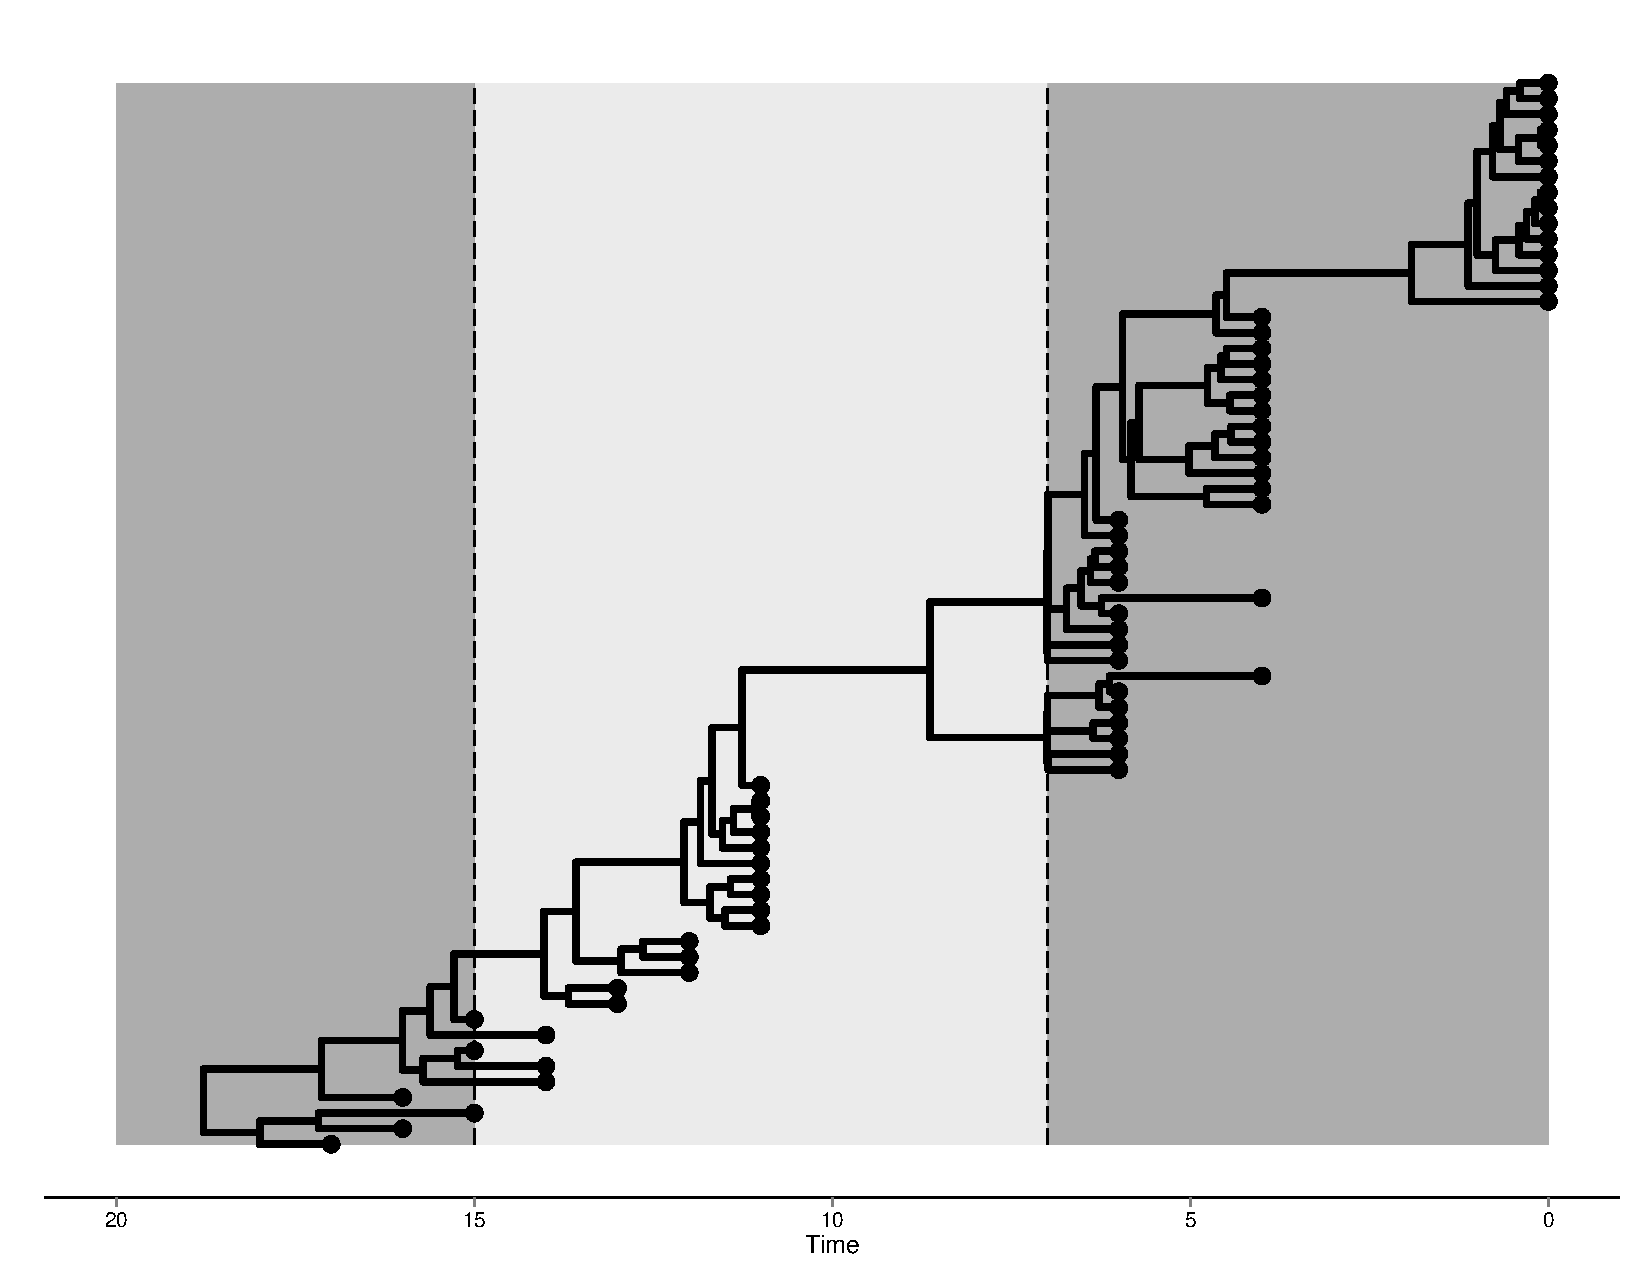
\includegraphics[scale=0.35]{threeEpoch} 
\caption{
{ \footnotesize 
{\bf Tree topology for time-heterogenous analysis.}
} % END: footnotesize
}
\label{fig:threeEpoch}
\end{figure}

The first epoch lasts until transition time $T_{1}$ set at $7$ (7 years before the most recent sampling date) and is governed by a model which we will call \textit{HKY$_1$}.
The second epoch lies between transition times $T_{1}$ and $T_{2}=15$, with substitution model \textit{HKY$_2$}. 
Finally, everything past $T_{2}$ occurs in a third epoch, with corresponding model \textit{HKY$_3$}.



\section{Turning BEAST's XML into an epochized analysis\label{sec:xml}}

Open the file generated in Section~\ref{sec:first} in your favourite text editor.
Scroll down to the block where the HKY model is defined.
We need to define three separate models for each epoch, corresponding to \textit{HKY$_1$}, \textit{HKY$_2$} and \textit{HKY$_3$}, therefore delete this block and paste there: 

\medskip{}

% TODO: update references to frequency model
\begin{lstlisting}
  <hkyModel id="hky.1">
    <frequencies>
      <frequencyModel idref="freqModel"/>
    </frequencies>
    <kappa>
      <parameter id="kappa.1" value="1.0" lower="0.0" upper="100.0"/>
    </kappa>
  </hkyModel>

  <hkyModel id="hky.2">
    <frequencies>
      <frequencyModel idref="freqModel"/>
    </frequencies>
    <kappa>
      <parameter id="kappa.2" value="1.0" lower="0.0" upper="100.0"/>
    </kappa>
  </hkyModel>
     
  <hkyModel id="hky.3">
    <frequencies>
      <frequencyModel idref="freqModel"/>
    </frequencies>
    <kappa>
      <parameter id="kappa.3" value="1.0" lower="0.0" upper="100.0"/>
    </kappa>
  </hkyModel>
\end{lstlisting}

\medskip{}

The individual models that will make up the epoch model are now available, so we can now setup the epoch model itself.
Below those three blocks paste:

\medskip{}

\begin{lstlisting}
  <epochBranchModel id="epochModel">
    <treeModel idref="treeModel"/>

    <epoch id="epoch1" transitionTime="10">
      <hkyModel idref="hky.1"/>
    </epoch>

    <epoch id="epoch2" transitionTime="15">
      <hkyModel idref="hky.2"/>
    </epoch>

    <hkyModel idref="hky.3"/>

  </epochBranchModel>
\end{lstlisting}

\medskip{}

Each {\color{darkblue}epoch} block references its corresponding model and transition time that bounds it, with the last (i.e., the furthest in the past) model being unbounded.
Now go to the line in the XML file where the site model is defined.
We need to reference the epoch model we just defined as our substitution model of choice.
Alter the corresponding line to have it look like this:

\medskip{}

\begin{lstlisting}
  <siteModel id="siteModel">
    <branchSubstitutionModel> 
      <beagleSubstitutionEpochModel idref="epochModel"/>
    </branchSubstitutionModel> 
  </siteModel>
\end{lstlisting}

\medskip{}

Now go to the {\color{darkblue}treeLikelihood} block in the XML file. 
This block also needs to reference the epoch model.
Change the corresponding line to read as follows:

\medskip{}

\begin{lstlisting}
  <treeLikelihood id="treeLikelihood">
    <patterns idref="patterns"/>
    <treeModel idref="treeModel"/>
    <siteModel idref="siteModel"/>
    <beagleSubstitutionEpochModel idref="epochModel"/>  
    <strictClockBranchRates idref="branchRates"/>
  </treeLikelihood>
\end{lstlisting}

\medskip{}

Since we now have three separate $\kappa$ parameters, we need to define separate transition kernels and separate prior distributions for each of these parameters.
Go to the {\color{darkblue}operators} block. 
Look for an operator which references kappa (our $\kappa$ parameter).
Delete this block and paste there:

\medskip{}

\begin{lstlisting}
  <scaleOperator scaleFactor="0.75" weight="0.1">
    <parameter idref="kappa.1"/>
  </scaleOperator>
		
  <scaleOperator scaleFactor="0.75" weight="0.1">
    <parameter idref="kappa.2"/>
  </scaleOperator>
		
  <scaleOperator scaleFactor="0.75" weight="0.1">
    <parameter idref="kappa.3"/>
  </scaleOperator>
\end{lstlisting}

\medskip{}

All the other parameters in this analysis are shared, therefore there is no need to define separate transition kernels for them.
Now look for the {\color{darkblue}prior} block, which you can find within the {\color{darkblue}mcmc} block.

We need three prior distributions, one per each $\kappa$ parameter (in this example we assume lognormally distributed $\kappa$ parameters):

\medskip{}

% \centering
\begin{lstlisting}
  <logNormalPrior mean="1.0" stdev="2" offset="0.0" meanInRealSpace="true">
    <parameter idref="kappa.1"/>
  </logNormalPrior>
				
  <logNormalPrior mean="1.0" stdev="2" offset="0.0" meanInRealSpace="true">
    <parameter idref="kappa.2"/>
  </logNormalPrior>
				
  <logNormalPrior mean="1.0" stdev="2" offset="0.0" meanInRealSpace="true">
    <parameter idref="kappa.3"/>
  </logNormalPrior>
\end{lstlisting}

\medskip{}

Naturally we want to log the three parameters of our epoch model. 
To monitor the analysis we start with the screen log. 
Look for the following line: <{\color{darkblue}log} {\color{darkblue}id}=\textquotedbl{}screenLog \textquotedbl{}{\color{darkblue}logEvery}=\textquotedbl{}5000\textquotedbl{}>.

Find the {\color{darkblue}column} block where the kappa parameter is referenced and paste these three blocks here instead:

\medskip{}

\begin{lstlisting}
  <column label="kappa.1" sf="6" width="12">
    <parameter idref="kappa.1"/>
  </column>
			
  <column label="kappa.2" sf="6" width="12">
    <parameter idref="kappa.2"/>
  </column>
			
  <column label="kappa.3" sf="6" width="12">
    <parameter idref="kappa.3"/>
  </column>
\end{lstlisting}

\medskip{}

We then still need to modify the lines responsible for storing the parameter estimates of the epoch model to file.
Go to the beginning of the {\color{darkblue}log} block responsible for keeping a log file, i.e. <{\color{darkblue}log} {\color{darkblue}id}=\textquotedbl{}fileLog\textquotedbl{} {\color{darkblue}logEvery}=\textquotedbl{}1000\textquotedbl{}>.
Find the line which references the \textit{kappa} parameter and paste there instead:

\medskip{}

\begin{lstlisting}
  <parameter idref="kappa.1"/>
  <parameter idref="kappa.2"/>
  <parameter idref="kappa.3"/>
\end{lstlisting}

\medskip{}

We are done with editing the XML and can proceed to performing the analysis.

\section{Running MCMC inference}

Epoch model inference requires the BEAGLE library installed and configured to be visible for BEAST.
Installation and setup of the BEAGLE library on various platforms is covered in \url{https://code.google.com/p/beagle-lib/w/list}.

In a UNIX/Linux environment, the XML edited in section \ref{sec:xml} can be run from the command line using the following command:

\begin{code}
java -Djava.library.path=/usr/local/lib -jar beast.jar epochExample.xml
\end{code}

\section{Analyzing the output}

After the analysis has finished you can import the resulting log file into the software of your choice, e.g. Tracer (a program for analysing the trace files generated by MCMC runs, \url{http://tree.bio.ed.ac.uk/software/tracer/}).

Figure \ref{fig:results} presents the posterior probability distributions of the $\kappa$ parameters, which were our main interest in this analysis. 
%GB: not sure why the line below was needed ...
%Bayesian credibility intervals for all parameter estimates contain the true values of the data.
We can clearly see non-overlapping regions, suggesting that the parameters $\kappa_1$ and $\kappa_3$ are significantly different from the parameter $\kappa_2$.
There is probably no difference between the parameters of the first and the third epoch.

\begin{figure}[h!]
\centering
% Tie Fighter plots!
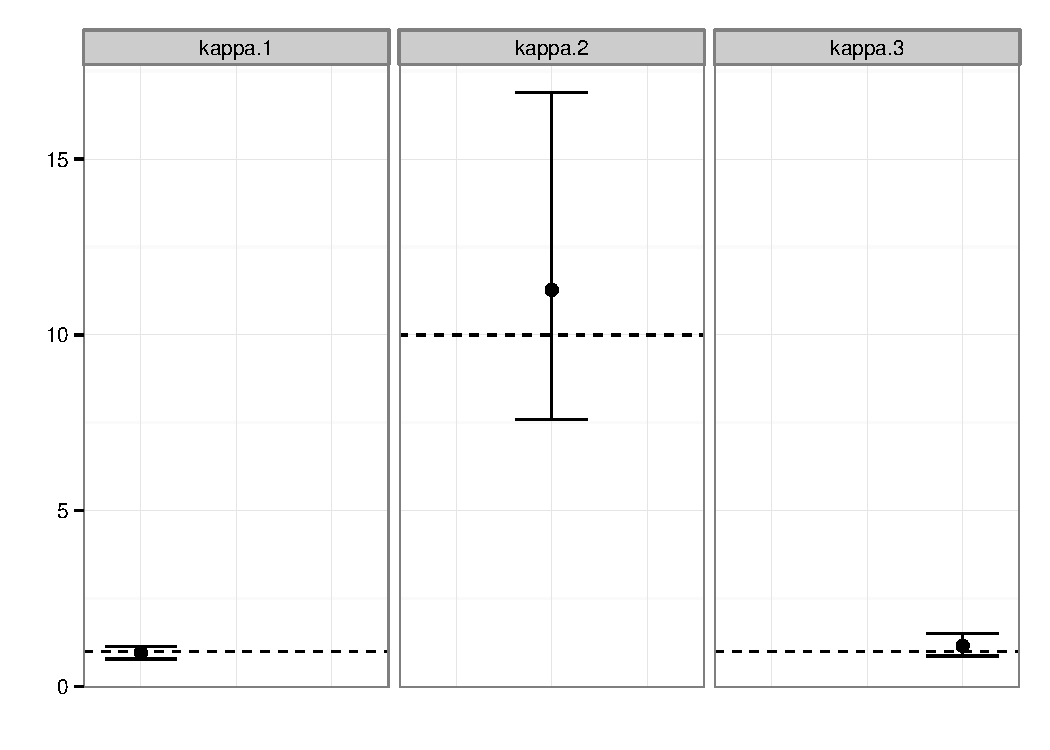
\includegraphics[scale=0.5]{results} 
\caption{
{ \footnotesize 
{\bf 95\% Credible intervals for $\kappa$ parameters.} Horizontal lines mark the true value, black dots indicate posterior mean values.
} % END: footnotesize
}
\label{fig:results}
\end{figure}












% \bibliography{epochtutorefs}
\cleardoublepage
\chapter{Tutorial on using SPREAD software\label{app:spread_tuto}}

% \begin{flushleft}
% \textbf{Authors}
% \par\end{flushleft}
% 
% \noindent
% Filip Bielejec (\url{filip.bielejec(sorry_spybots)rega.kuleuven.be}) \\
% Philippe Lemey (\url{philippe.lemey(sorry_spybots)rega.kuleuven.be}) \\
% Andrew Rambaut (\url{a.rambaut(sorry_spybots)ed.ac.uk}) \\
% Marc Suchard (\url{msuchard(sorry_spybots)ucla.edu})\\

\begin{flushleft}
\textbf{Download}
\par\end{flushleft}
Compiled, runnable program can be downloaded from: \url{http://www.phylogeography.org/SPREAD.html}
Get the source code on GitHub: \url{https://github.com/phylogeography/SPREAD}.
You can also clone the project with Git by running:

\begin{lyxcode}
git~clone~git@github.com:phylogeography/SPREAD.git
\end{lyxcode}
% \pagebreak{}

\section{Introduction}

In this supplement we give a detailed description of program functionalities, describe some possible analysis and give general guidelines on running Spread. 
We present an example for each of the possible analysis. 
The example files used in the analysis can be accessed from \url{http://www.phylogeography.org/SPREAD.html}.
The generated visualisations can be opened for viewing in Google Earth (\url{www.google.com/earth/}) or any other GIS software capable of reading the Keyhole Markup Language (KML) format.


\section{Recommended platform, hardware and software for Spread}

Spread will run on a variety of platforms, as long as a suitable Java
Runtime Environment is present. Recommended JRE include OpenJDK and
Sun JRE, however application will also run on other runtime environments.
Spread has been tested on well established operating systems namely
Debian GNU/Linux, Mac OS X, Windows XP, as well as more esoteric ones
like Nokia Linux Maemo 5 and Linux MeeGo. For most of the templates
following hardware is sufficient: 

\begin{itemize}
\item CPU: Intel CPU 600 MHz or above
\item Main Memory: 1 GB or above
\item Runtime Environment: Sun Java Runtime Environment or OpenJDK 
\end{itemize}
The Time Slicer analysis is more resource-hungry and therefore we
recommend running it with following hardware:
\begin{itemize}
\item CPU: Intel Core 2 Duo 2.0 Ghz or above
\item Main Memory: 3 GB or above
\item Runtime Environment: Sun Java Runtime Environment or OpenJDK 
\end{itemize}

\section{Visualizing location annotated MCC tree}

This tutorial assumes the user has generated the location annotated
Maximum Clade Credibility (MCC) tree. 
Good tutorial on doing so can be found in Tree Summary section of BEASTs tutorial wiki: 

\url{http://beast.bio.ed.ac.uk/Tree_summary} 

\noindent
The example tree file and location coordinates file for this analysis can be found here:

\url{http://www.kuleuven.be/aidslab/phylogeography/SPREAD_files/H5N1_HA_discrete_MCC.tre}

\noindent
and here: 

\url{http://www.kuleuven.be/aidslab/phylogeography/SPREAD_files/locationCoordinates_H5N1.txt}

\noindent
This example considers influenza A H5N1 diffusion among 7 discrete locations. 
We will visualise this data using Spread own map and virtual globe software. 


\subsection{Loading the data}

Click on the Discrete Model tab, then on the Load tree file button
and navigate to the location of your MCC tree file to load it.

\begin{figure}[H]
\begin{centering}
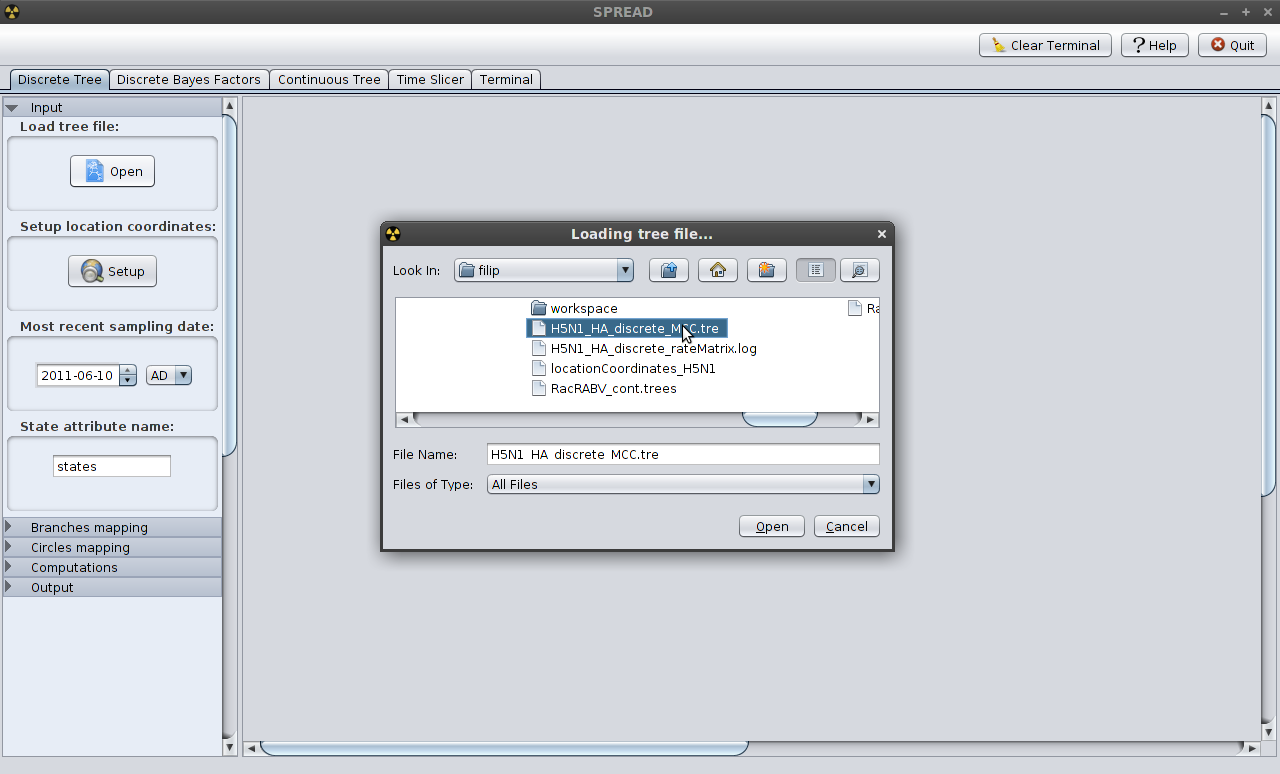
\includegraphics[scale=0.25]{fig01}
\par\end{centering}
\caption{Loading MCC tree file.}
\label{fig:01}
\end{figure}


The Spread will now set the working directory to the one containing
your file. This means that the generated KML output will be saved
in that directory.

\begin{figure}[H]
\begin{centering}
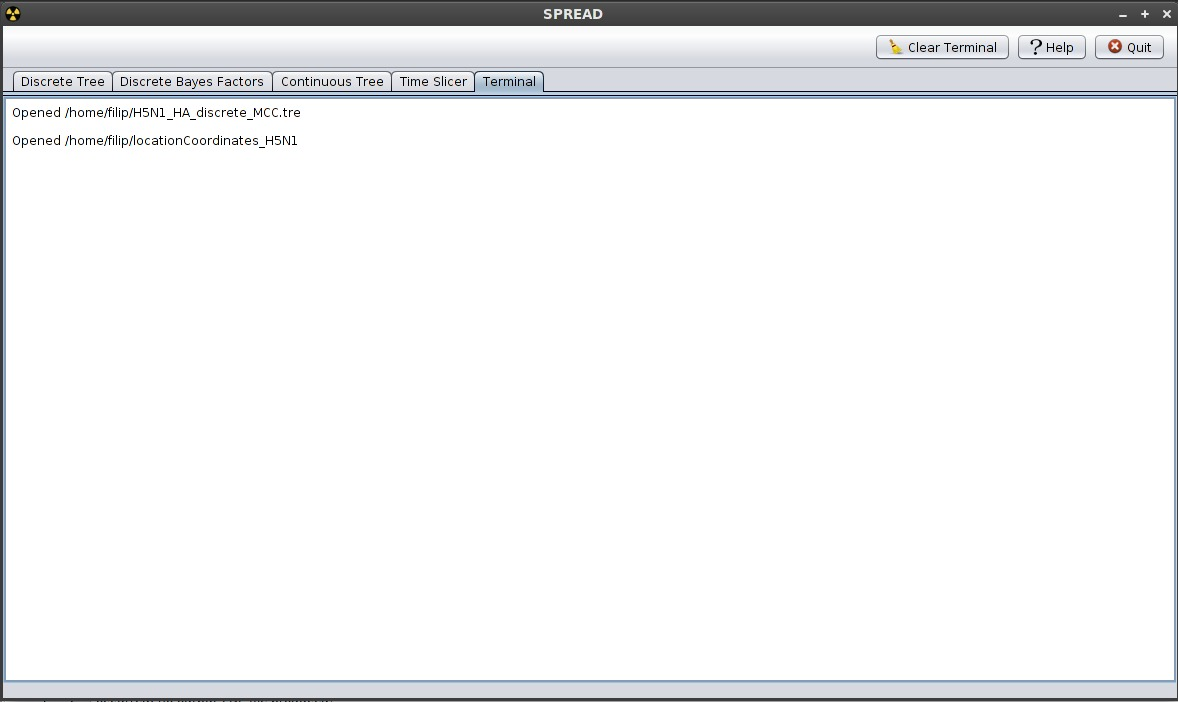
\includegraphics[scale=0.25]{fig02}
\caption{Message in Terminal.}
\label{fig:02}
\par\end{centering}
\end{figure}


To view the MCC tree in it's geographic context, we have to associate
each location with a particular latitude and longitude. To this purpose,
you can either use the editor supplied with Spread and generate the
input file or load previously prepared tab-delimited file including
each location, its latitude and longitude. For the H5N1 example, the
file should look like this:

\begin{lyxcode}
% \centering
Fujian~25.917~118.283

Guangdong~22.87~113.483

Guangxi~23.6417~108.1

Hebei~39.3583~116.6417

Henan~33.875~113.5

HongKong~22.3~114.167

Hunan~27.383~111.517
\end{lyxcode}

\begin{figure}[H]
\begin{centering}
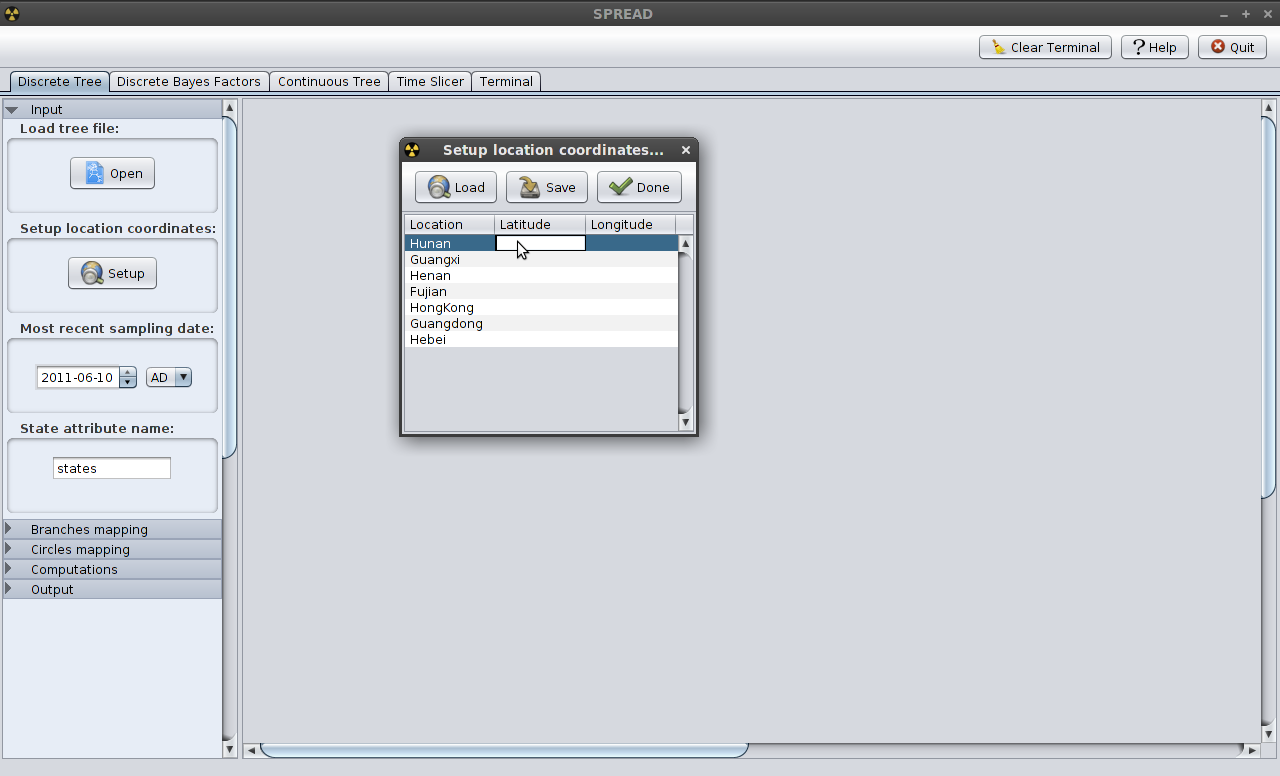
\includegraphics[scale=0.25]{fig003}
\caption{Location coordinates editor.}
\label{fig:003}
\par\end{centering}
\end{figure}

Go to the Discrete Model tab and click on Setup location coordinates
button. You should see the list of discrete locations parsed from
your tree. Click on the appropriate fields and fill them with latitude
and longitude coordinates. After you finished editing the file save
it and load it by clicking on Done button. Alternatively use the Load
button and navigate to your previously prepared location coordinates
file to load it. 

In either case when you click on Done button the Terminal tab should
show You how many discrete locations have been read by Spread, with
their names and corresponding latitude and longitude coordinates.
If you forgot to save the edited file You can still copy and paste
this output.

\begin{figure}[H]
\begin{centering}
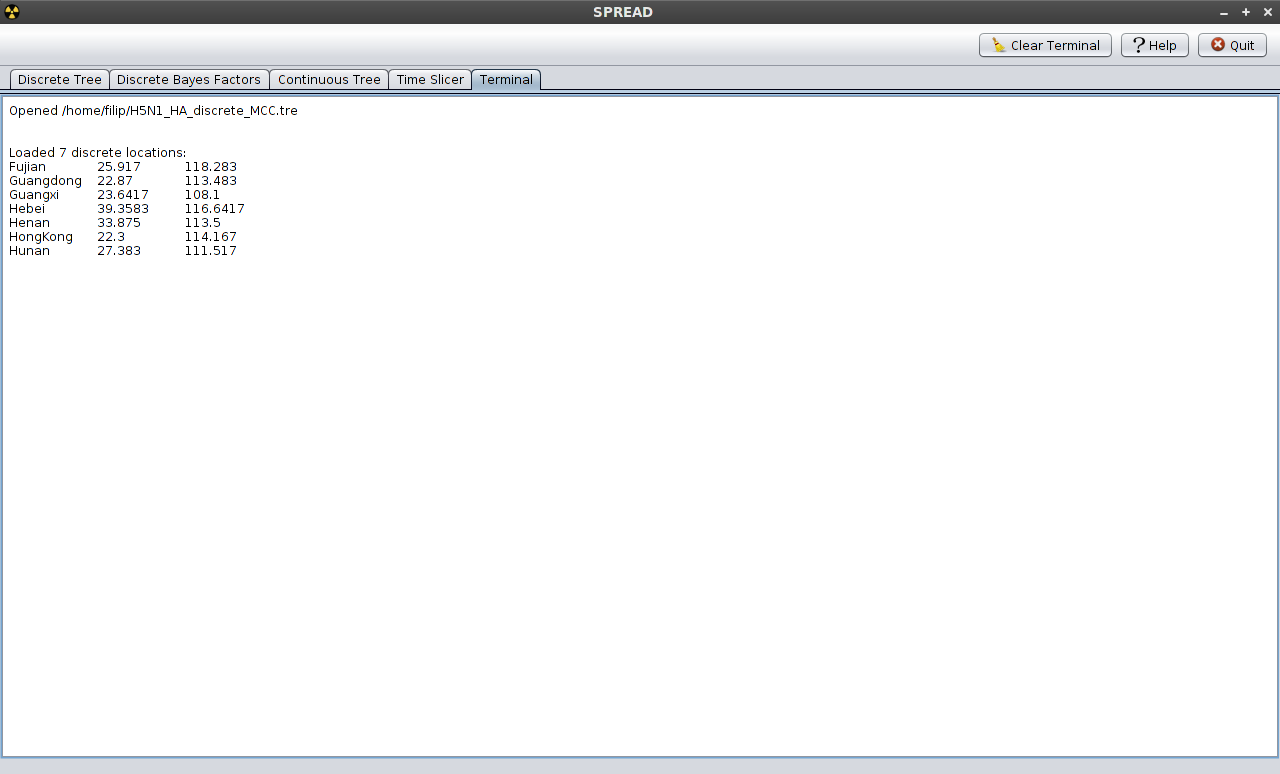
\includegraphics[scale=0.25]{fig0003}
\caption{Terminal output.}
\label{fig:0003}
\par\end{centering}
\end{figure}

\subsection{Setting the visualisation attributes}

Now that your data is loaded, you can start setting the attributes.

\begin{itemize}
\item \textbf{Most recent sampling date} (mrsd) is specified in YYYY-MM-DD
format. If You know only the year set it to the last day of the previous
year. Use the spinner to operate Year, Month and Day fields. You can
also choose whether the date is in our era (AD), or not (BC).
\item \textbf{State attribute name} is the name of tree nodes discrete locations
attribute. Common names include \textsl{state} or \textsl{states}.
Specify it accordingly, otherwise Spread would be unable to parse
the data correctly. If in doubt you can always open your tree in a
text editor and check for the attribute name. H5N1 analysis uses the
default name. 
\item \textbf{Branches color mapping} allows you to setup the minimal and
maximal colors of the plotted lines. Spread will map the node heigth
values of the MCC tree to the colors in between the specified maximal
and minimal boundary. Set both mappings to the same color if you want
no mapping assigned.
\item Adjust the size of lines using the \textbf{Branches width} slider.
\item \textbf{Circles color mapping} allows you to setup the minimal and
maximal colors of the plotted circular polygons. Those polygons will
have their colors mapped accordingly to the number of lineages holding
the discrete state at the given time (interval). You can choose the
beginning and the end values of those color mappings, by specifying
RGB, HSB opacity and brightness values.
\item The radius of circular polygons represents the number of lineages
holding the discrete state at a given time. The default value of 100
times the square root of the number of lineages can be multiplied
by a choosen constant using \textbf{Circles radius multiplier}.
\item \textbf{Number of intervals} specifies into how many intervals your
MCC tree timeline (time from tree root until the most recent sampling
date) will be cutted into. 100 intervals is a good default value for
most applications.
\item \textbf{Maximal altitude mapping} refers to the KML output. Spread
will map the geographic distances between discrete locations to the
altitude of the lines connecting them, giving higher altitudes to
the distant ones and lower altitudes to the ones lying close to each
other. Changing this attribute will modify the upper boundary of the
mapping. If you set it to 0 all lines will be flat.
\item \textbf{KML name} field allows you to specify the name of the output
file.
\end{itemize}


\begin{figure}[H]
\begin{centering}
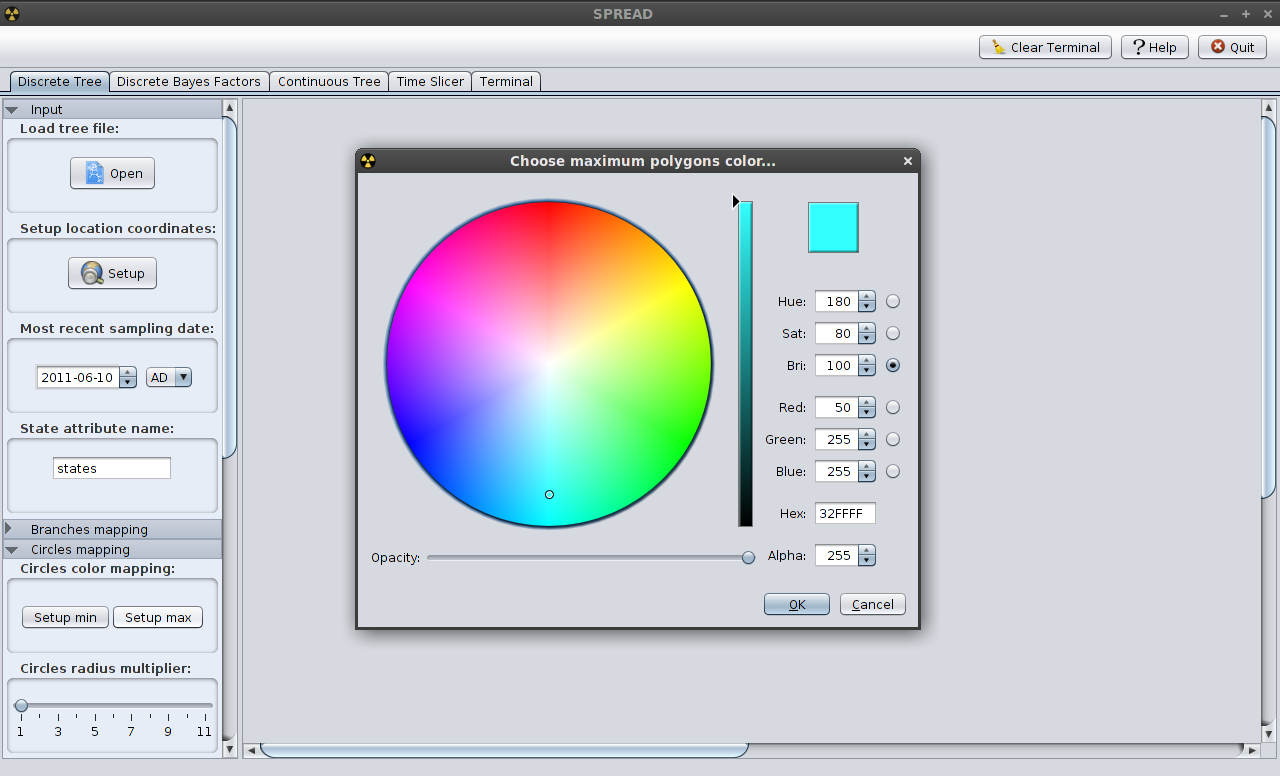
\includegraphics[scale=0.25]{fig03}
\caption{Color chooser.}
\label{fig:03}
\par\end{centering}
\end{figure}


\subsection{Generating the visualisations}

Once you're satisfied with the specified attributes click on Generate
KML button to generate output for viewing in virtual globe software.
If everything went fine you should see a message in Terminal tab indicating
how long did it take for Spread to generate the file. If something
went wrong Spread will also show a warning or an error message there.


\begin{figure}[H]
\begin{centering}
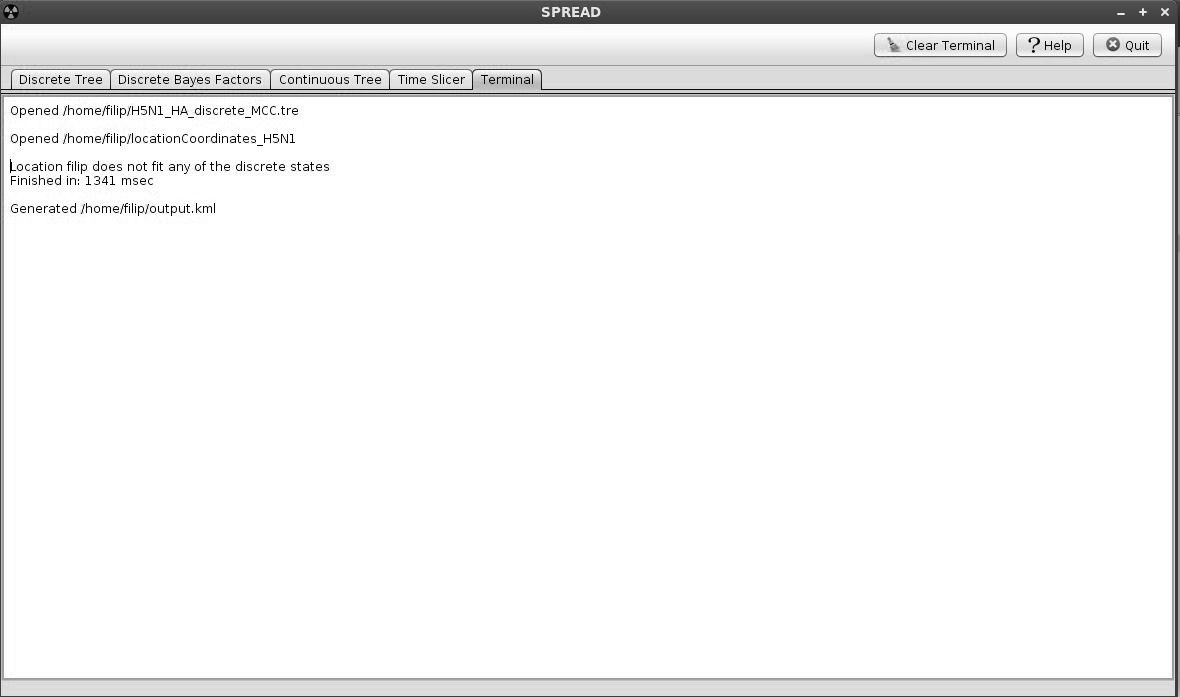
\includegraphics[scale=0.25]{fig04}
\caption{Message in Terminal.}
\label{fig:04}
\par\end{centering}
\end{figure}

The visualisation once opened for viewing in Google Earth (GE) will
have a slider indicating the time component of the phylogeny. Clicking
on the play button starts an animation of the viral diffusion over
time. 

Click on Plot map button in Spread menu to view the visualisation
in the inner Spread map. 


\begin{figure}[H]
\begin{centering}
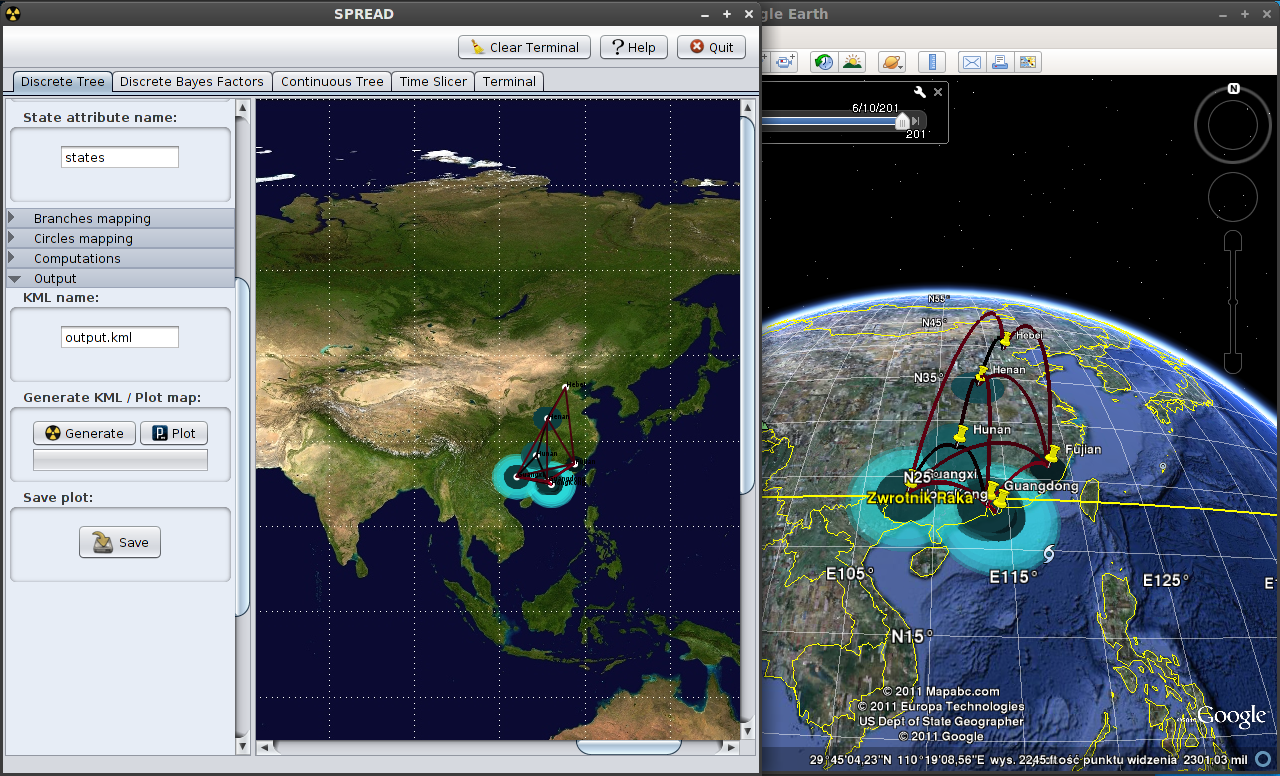
\includegraphics[scale=0.25]{H5N1_discrete_vis}
\caption{Screenshot of the Spread output.}
\label{fig:05}
\par\end{centering}
\end{figure}

\section{Identifying well supported rates using Bayes factors test}

This tutorial assumes the user has generated a BEAST log file with
rate indicators as described in Bayesian stochastic search variable
selection (BSSVS) procedure, as described here:

\url{http://beast.bio.ed.ac.uk/BSSVS} 

\noindent
The test aims at identifying frequently invoked rates to explain the
diffusion process and visualize them in virtual globe software or
using Spread own map. 

\noindent
The log file used in this example can be accessed from here:

\url{http://www.kuleuven.be/aidslab/phylogeography/SPREAD_files/H5N1_HA_discrete_rateMatrix.log}

\noindent
The location coordinates file can be downloaded using the following
url: 

\url{http://www.kuleuven.be/aidslab/phylogeography/SPREAD_files/locationCoordinates_H5N1.txt}.


\subsection{Loading the data}

Go to the Rate Indicator BF tab and load your log using proper button
and a supplied chooser, to navigate to the directory containing your
log file. 

\begin{figure}[H]
\begin{centering}
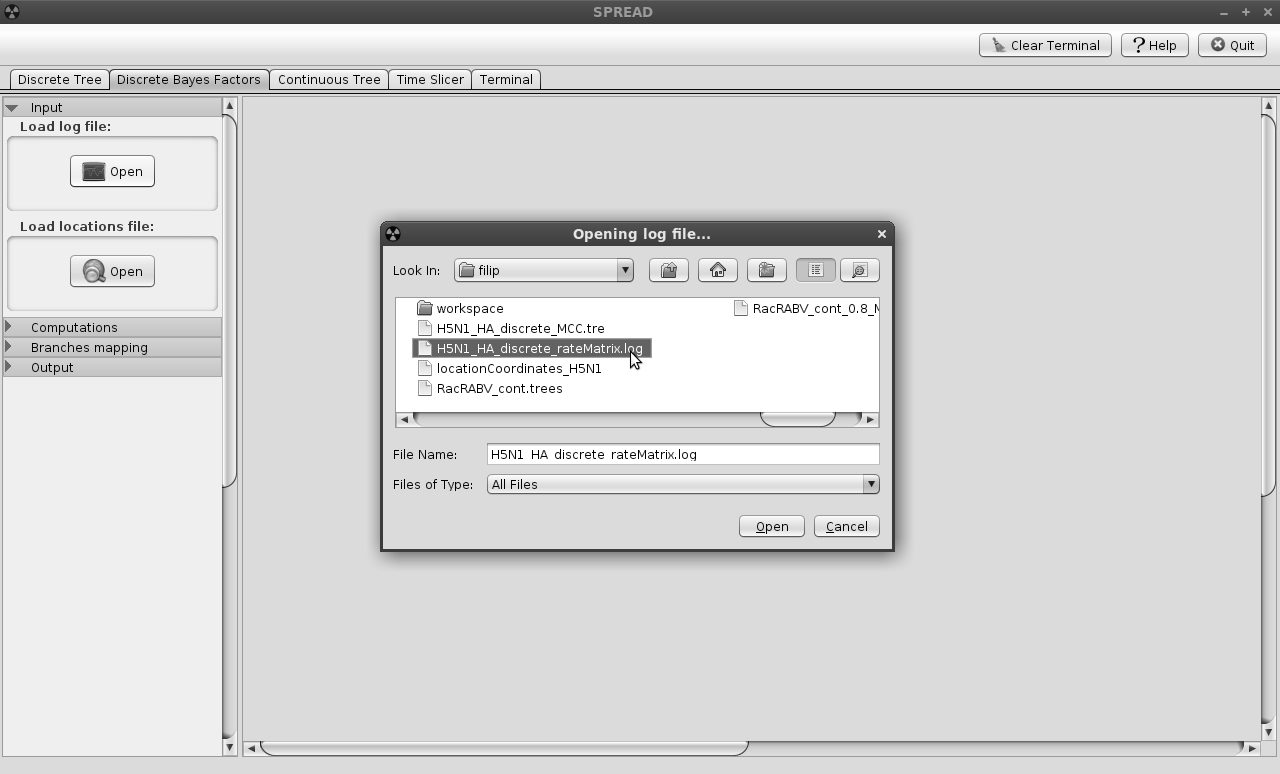
\includegraphics[scale=0.25]{fig06}
\caption{Loading the log file.}
\label{fig:06}
\par\end{centering}
\end{figure}

To analyze the results in the log file we will need a tab delimited
file with location names and their latitude and longitude coordinates.
For H5N1 analysis example this file should look like this:

\begin{lyxcode}
Fujian~25.917~118.283

Guangdong~22.87~113.483

Guangxi~23.6417~108.1

Hebei~39.3583~116.6417

Henan~33.875~113.5

HongKong~22.3~114.167

Hunan~27.383~111.517
\end{lyxcode}

You can either use the location coordinates editor to prepare it,
or load a previously saved file. In either case when you click on
Done button the Terminal tab should show you how many discrete locations
have been read by Spread, with their names and corresponding latitude
and longitude coordinates. If you forgot to save the edited file you
can still copy and paste this output.

\begin{figure}[H]
\begin{centering}
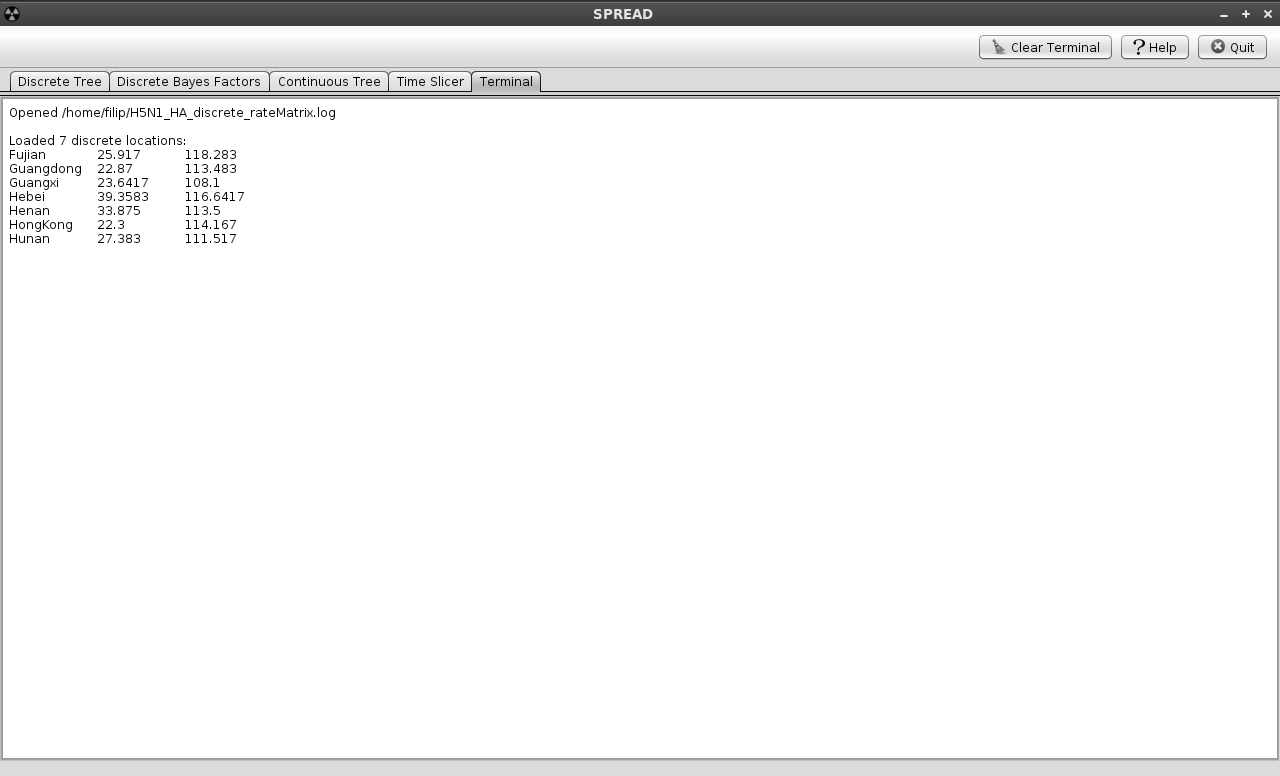
\includegraphics[scale=0.25]{fig006}
\caption{Terminal output.}
\label{fig:006}
\par\end{centering}
\end{figure}

\subsection{Setting the visualisation attributes}

Now that your data is loaded, you can start setting the attributes.

\begin{itemize}
\item Use \textbf{Specify burn-in} slider to set how many initial samped
values should be discarded from the analysis. The default value of
10\% should be sufficient for most of the analysis.
\item \textbf{Poisson prior mean/offset} specifies the mean of the (truncated)
Poisson prior (the default value is $log(2)$ unless specified otherwise)
and the offset of the (truncated) Poisson prior (the default is the
number of locations - 1 unless specified otherwise).
\item \textbf{Bayes factor cut-off} specifies the Bayes factor values above
which we consider rates to be well supported (only those rates will
be visualised). For H5N1 analysis the default cut-off of 3.0 is sufficient. 
\item \textbf{Rates color mapping} allows you to setup the minimal and maximal
colors of the plotted lines. Spread will map the log of bayes factors
values to the colors in between the specified maximal and minimal
boundary.
\item Adjust the size of lines using the \textbf{Rates width} slider.
\item \textbf{Number of intervals} is a purely technical attribute and specifies
of how many line segments your rate lines will consist of, setting
this number too small can result in crude looking lines. We suggest
leaving the default value of 100.
\item \textbf{Maximal altitude mapping} refers to the KML output. Spread
will map the geographic distances between discrete locations to the
altitude of the lines connecting them, giving higher altitudes to
the distant ones and lower altitudes to the ones lying close to each
other. Changing this attribute will modify the upper boundary of the
mapping. If you set it to 0 all lines will be flat.
\item \textbf{KML name} field allows you to specify the name of the output
file.
\end{itemize}

\subsection{Generating the visualisations}

Once you're happy with the specified plotting attributes click on
the Generate KML button. Spread will now output the kml file in its
current working directory, you can view this file using google Earth
or any other software capable of reading the format. You can also
see the visualisation using Spreads own map by clicking the Plot button.

\begin{figure}[H]
\begin{centering}
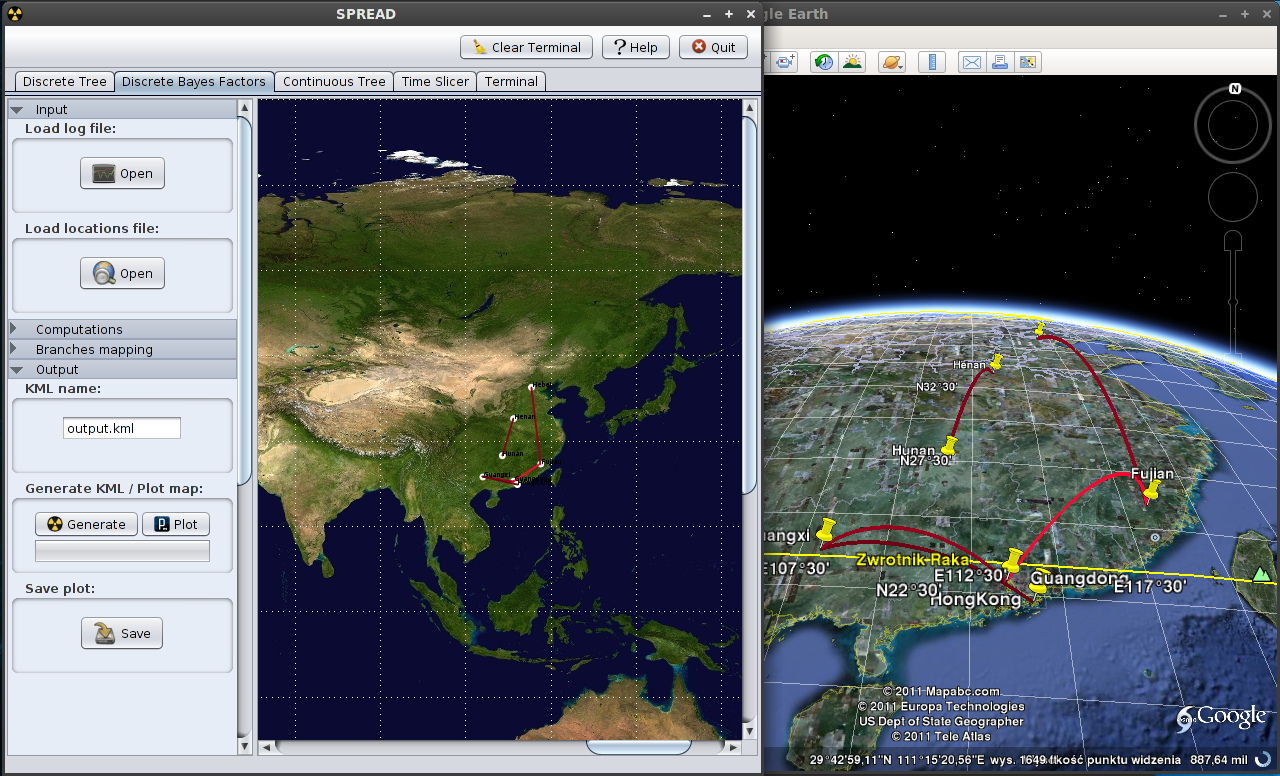
\includegraphics[scale=0.25]{H5N1_bf_vis}
\caption{Generated visualisations.}
\label{fig:07}
\par\end{centering}
\end{figure}

Both plotting and generating kml output file should result in a lists
with the rates yielding a bayes factor above the specified cut-off
to be printed in the terminal tab. You copy and paste this output
for later use. The rates are by default sorted in ascending order.


\begin{figure}[H]
\begin{centering}
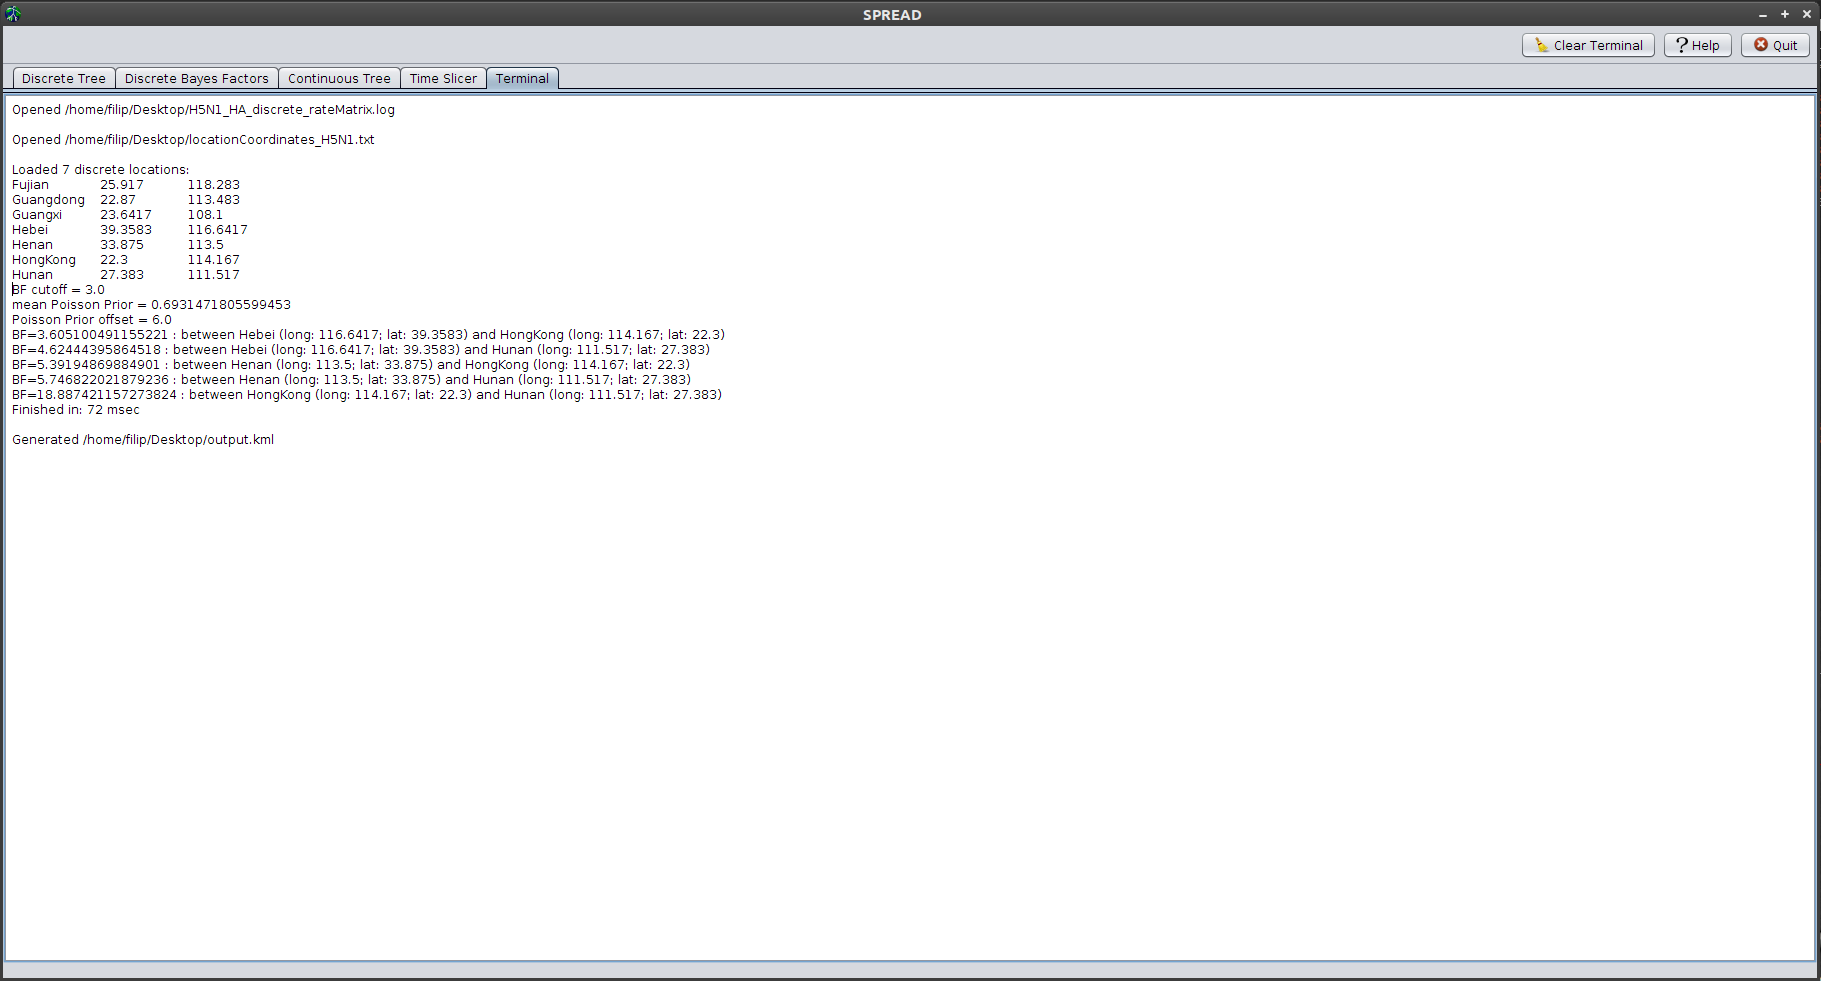
\includegraphics[scale=0.2]{fig08}
\caption{Terminal tab output.}
\label{fig:08}
\par\end{centering}
\end{figure}

\section{Visualising a continuous MCC tree}

This tutorial assumes the user has set up a BEAST phylogeographic
analysis in continuous space and generated a Maximum Clade Credibility
(MCC) tree using TreeAnnotator. Good tutorial on neccessary steps
can be found here:

\url{http://beast.bio.ed.ac.uk/Continuous_phylogeographic_analysis}

\noindent
This visualisation aims at projecting the MCC tree on the grid of
geographical coordinates, with polygons representating the uncertainty
in location coordinates and considers raccoon rabies diffusion in
north-eastern United States. 
The example tree file used in the presented analysis can be accessed
from here:

\url{http://www.kuleuven.be/aidslab/phylogeography/SPREAD_files/RacRABV_cont_0.8_MCC_snyder.tre}


\subsection{Loading the data}

Click on Continous model tab and load your MCC tree into Spread. If
you now open the Terminal tab Spread will show message with path to
your file, indicating it has set the working directory to the one
your file is in (generated output will go there).

\begin{figure}[H]
\begin{centering}
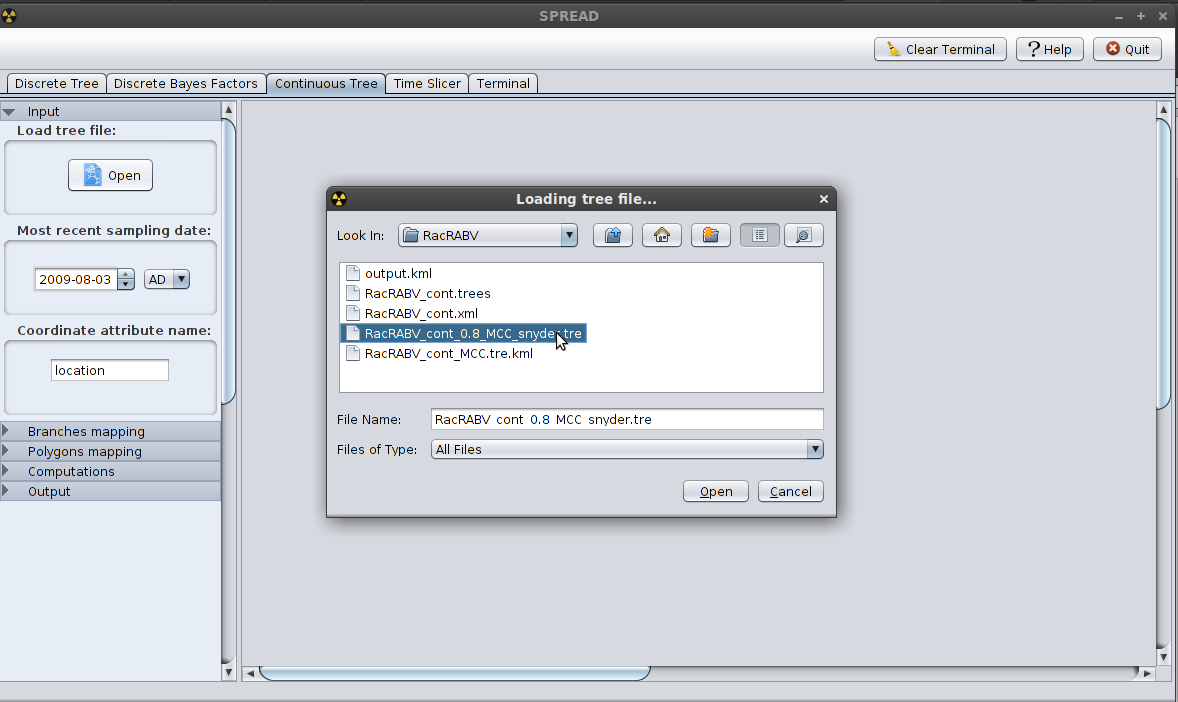
\includegraphics[scale=0.25]{fig09}
\caption{Loading tree file.}
\label{fig:09}
\par\end{centering}
\end{figure}

\subsection{Setting the visualisation attributes}

\begin{itemize}
\item \textbf{Most recent sampling date} (mrsd) is specified in YYYY-MM-DD
format. If you know only the year set it to the last day of the previous
year. Use the spinner to operate Year, Month and Day fields. You can
also choose whether the date is in our era (AD), or not (BC). 
\item \textbf{Coordinate attribute name} is the name of tree nodes coordinate
attribute. Common names include \textsl{location} or \textsl{trait}.
Specify it accordingly, otherwise Spread would be unable to parse
the data correctly. If in doubt you can always open your tree in a
text editor and check what's that attribute name. Racoon rabies data
that we will use in this tutorial uses \textsl{location }as the attribute
name.
\item \textbf{Branches color mapping} allows you to setup the minimal and
maximal color values of the plotted lines. Spread will map the node
heigth values of the MCC tree to the colors in between the specified
set, what results in the continuous color gradient on your visualisation.
\item Adjust the size of branch lines using the \textbf{Branches width}
slider.
\item \textbf{Maximal altitude mapping} refers to the KML output. Spread
will map the geographic distances between discrete locations to the
altitude of the lines connecting them, giving higher altitudes to
the distant ones and lower altitudes to the ones lying close to each
other. Changing this attribute will modify the upper boundary of the
mapping. If you set it to 0 all lines will be flat.
\item \textbf{Polygons color mapping} allows you to setup the minimal and
maximal colors of the plotted polygons. Those polygons will have their
colors mapped accordingly to the relative time of the dispersal pattern.
You can choose the beginning and the end values of those color mappings,
by specifying RGB, HSB, opacity and brightness values.
\item \textbf{Number of intervals} specifies into how many intervals your
timeline (time from tree root until the most recent sampling date)
should be cut into. 100 intervals is a good default value for most
visualisations.
\item \textbf{KML name} field allows you to specify the name of the output
file.
\end{itemize}

\subsection{Generating the visualisations}

Once you're satisfied with the specified attributes click on Generate
KML button to generate output for viewing in virtual globe software.
If everything went fine you should see a message in the Terminal tab
indicating how long did it take for Spread to generate the file. The
generated output can now be opened for viewing in Google Earth. Once
opened in GE visualisation will have a slider indicating the time
component of the tree. Clicking on the play button starts an animation
of the viral diffusion through time. Click on Plot map button in Spread
menu to view the visualisation in the inner Spread map.

\begin{figure}[H]
\begin{centering}
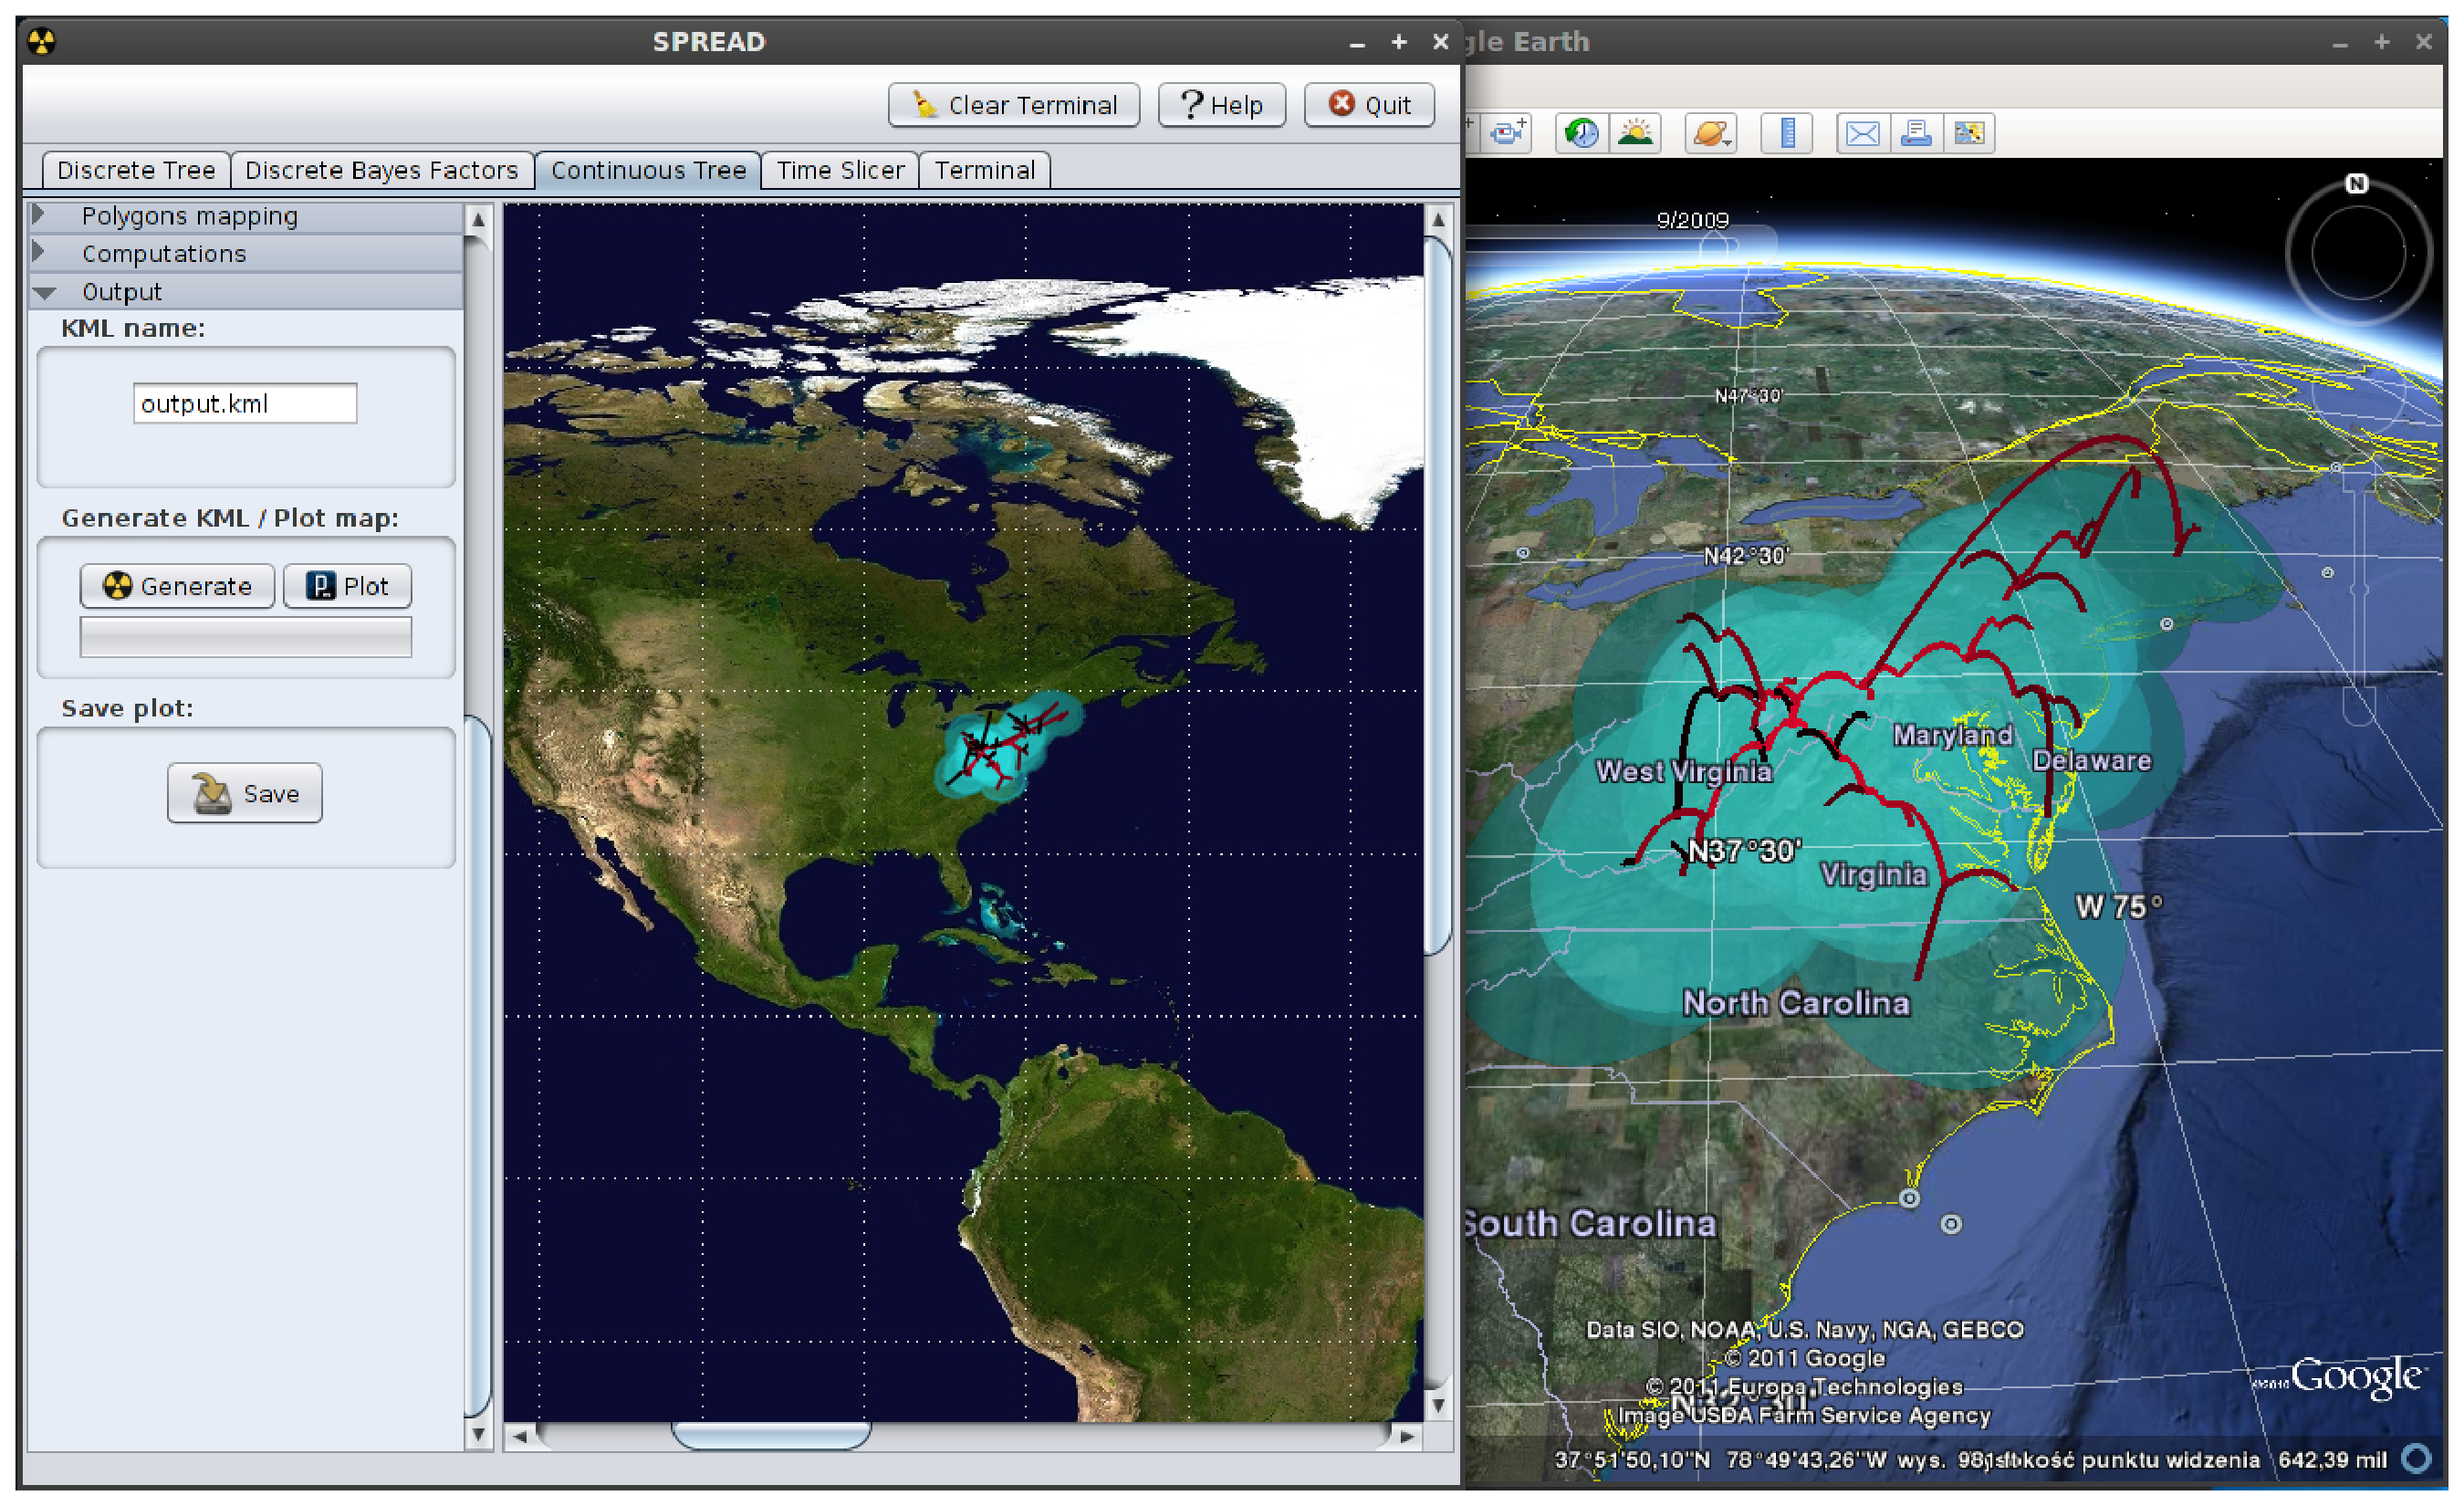
\includegraphics[scale=0.25]{RacRABV_cont_vis}
\caption{TScreenshot of the Spread output.}
\label{fig:RacRABV_cont_vis}
\par\end{centering}
\end{figure}

\section{Summarising full posterior distribution}

This tutorial assumes the user has set up a BEAST phylogeographic
analysis in continuous space and generated a trees file and an MCC
tree file using TreeAnnotator. Good tutorial on neccessary steps can
be found here:

\url{http://beast.bio.ed.ac.uk/Continuous_phylogeographic_analysis}

\noindent
This analysis allows one to summarise and visualise full posterior
distribution of the trees obtained in continuous phylogeographic analysis.
To achieve this Spread creates a time line according to the MCC tree
length, slices through each phylogeny at a particular points in time,
imputes the unobserved descendant locations for those time points
and contoures them by creating polygons, a natural representation
of the uncertainty in these inferences. In this template we also visualise
the MCC tree which gave rise to the time slices by drawing it's branches.

Since Spread version 1.0.2 user can choose to supply custom slice
heights instead of automatically defining them according to the MCC
tree. This can be done by choosing appropriate analysis type and then
loading text file with the custom slice times.

\begin{figure}[H]
\begin{centering}
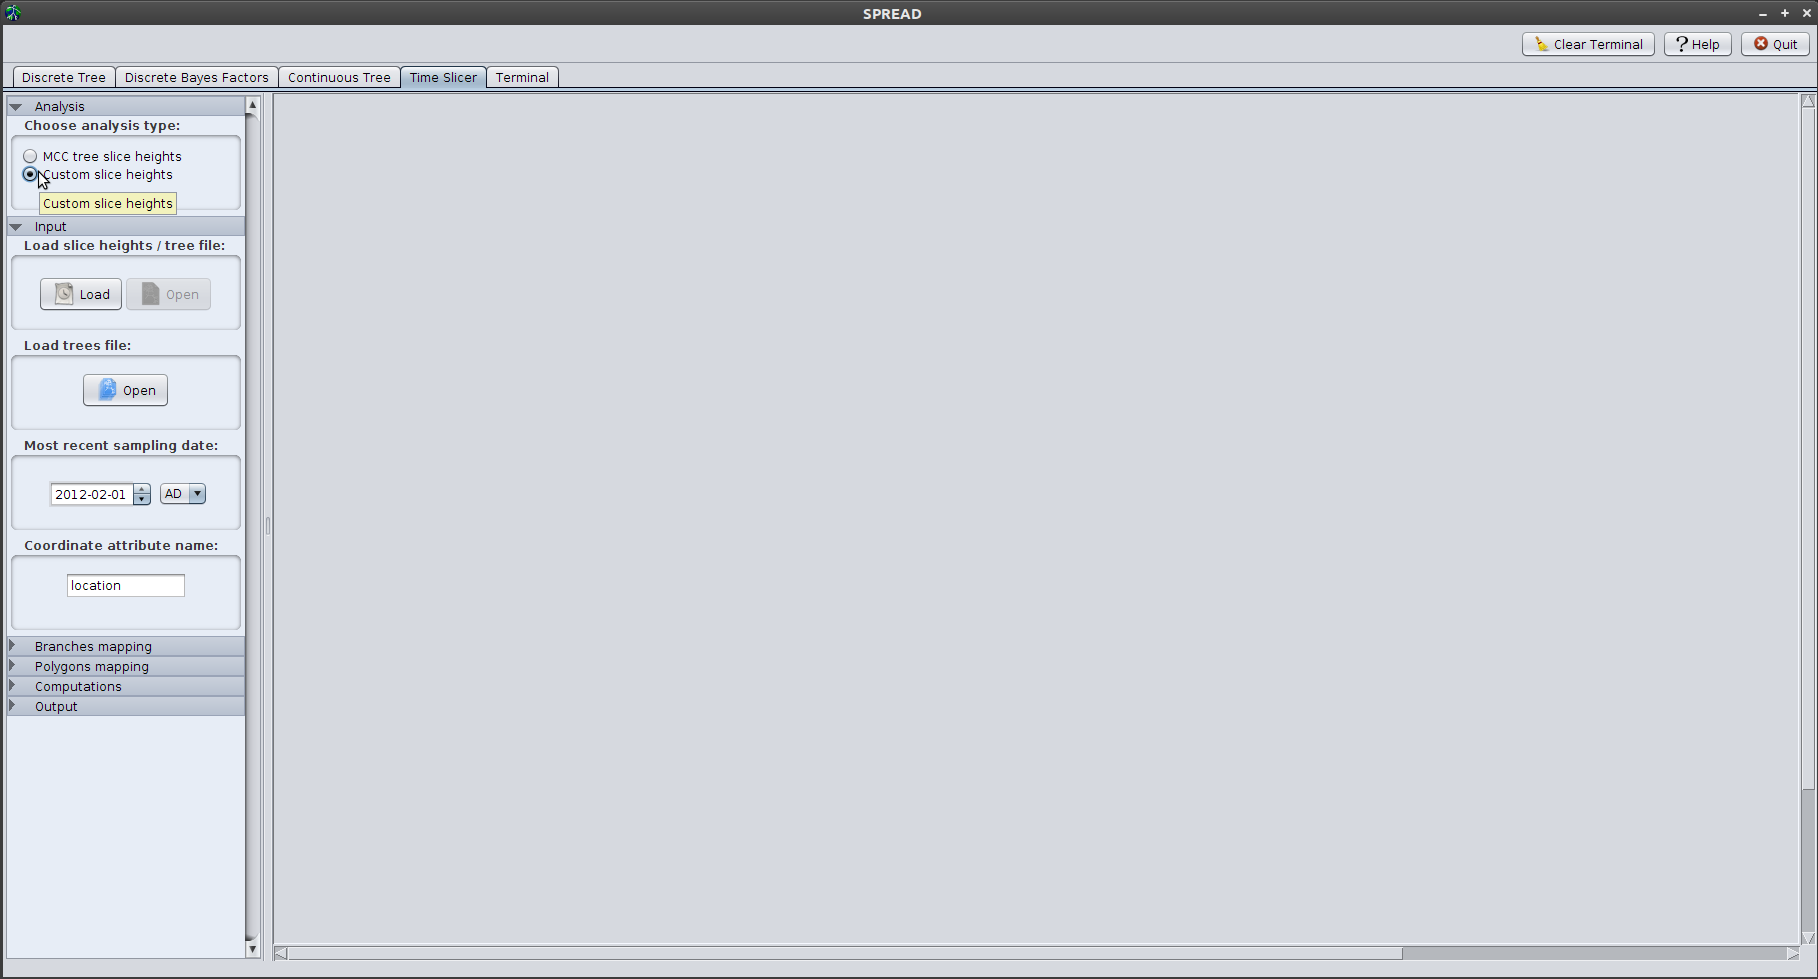
\includegraphics[scale=0.2]{fig10}
\caption{Choosing analysis type.}
\label{fig:10}
\par\end{centering}
\end{figure}

We will use the same racoon rabies data as in the continuous tree
visualisation. The tree files used in this analysis can be downloaded
from:

\url{http://www.kuleuven.be/aidslab/phylogeography/SPREAD_files/RacRABV_cont_0.8_MCC_snyder.tre}

\noindent
and the trees file from:

\url{http://www.kuleuven.be/aidslab/phylogeography/SPREAD_files/RacRABV_cont.trees}

\noindent
Note that this analysis is much more resource-hungry and you might
want to increase the heap space availiable for the Java Virtual Machine.
This can be done by starting Spread from command line with the following
arguments: 

\begin{lyxcode}
java~-jar~-Xmx2024m~spread.jar
\end{lyxcode}

\subsection{Loading the data}

First you need to load the MCC tree that gives rise to the time intervals.
Do this using the Load tree file button. Next import the trees file
using Load trees file button. Once you're done start setting the appropriate
attributes.


\subsection{Setting the visualisation attributes}

Now that your data is loaded, you can start setting the plotting attributes.
Time Slicer template allows for the following options to be specified: 

\begin{itemize}
\item \textbf{Most recent sampling date }(mrsd) is specied in YYYY-MM-DD
format. Use the spinner to operate Year, Month and Day fields. You
can also choose whether the date is in our era (AD), or not (BC). 
\item \textbf{Coordinate attribute name} is the name of tree nodes coordinate
attribute. Specify it correctly, otherwise Spread would be unable
to parse the data correctly, what results in error message.
\item \textbf{Branches color mapping} allows you to setup the minimal and
maximal color values of the plotted lines. Spread will map the node
heigth values of the MCC tree to the colors in between the specified
maximal and minimal boundary what results in the continuous color
gradient for those values.
\item \textbf{Branches width} slider allows to adjust the size of branch
lines.
\item \textbf{Maximal altitude mapping} refers to the KML output. Spread
will map the geographic distances between discrete locations to the
altitude of the lines connecting them, giving higher altitudes to
the distant ones and lower altitudes to the ones lying close to each
other. Changing this attribute will modify the upper boundary of the
mapping. If you set it to 0 all lines will be flat.
\item \textbf{Polygons color mapping} allows you to setup the minimal and
maximal colors of the plotted polygons. Those polygons will have their
colors mapped accordingly to the relative time of the dispersal pattern.
You can choose the beginning and the end values of those color mappings,
by specifying RGB, HSB opacity and brightness values.
\item You can choose the \textbf{Use true noise} checkbox if you wish to
interpolate between the imputed locations. You then have to specify
the appropriate \textbf{Rate attribute name} and \textbf{Precision
attribute name}, using the text fields.
\item \textbf{Specify burn-in} is the field in which you let the Spread
know how many initial trees should be discarded from the analysis. 
\item Use highest posterior density \textbf{(HPD}) field to specify the
level of the kernel density estimation. Common values used are 0.8,
0.95 and 0.99.
\item \textbf{Number of intervals} specifies into how many intervals your
timeline (time from the root of the phylogeny until the most recent
sampling date) should be cut into. 100 intervals is a good default
value for most visualisations.
\item \textbf{Grid size} slider lets you adjust the number of points used
in contouring. In general the larger the value the smoother the generated
polygons will be, however the analysis also gets more computationally
involved as this value increases.
\item \textbf{KML name} field allows you to specify the name of the output
file.
\end{itemize}

\subsection{Generating the visualisations}

When you are satisfied with specified attributes click on the Generate
KML button to export the results to keyhole markup language or the
Plot button to visualise them on a map. Depending on the size of your
data the analysis might take some time. You can observe the progress
and errors if any, in the Terminal tab.

Once Spread is done you can open the resulting kml file in the virtual
globe software and animate the spatial diffusion over time.

\begin{figure}[H]
\begin{centering}
\includegraphics[scale=0.25]{RacRABV_Time_Slicer_vis}
\caption{Terminal tab output.}
\label{fig:12}
\par\end{centering}
\end{figure}

\section{Tips \& tricks}

For some Mac users Spread refuses to generate KML output of the Bayes
factors test, even though it claims to have done so in the Terminal
output. This problem can be fixed by starting Spread with more memory
availliable. To do so start Spread from command line with the following
arguments: 

\begin{lyxcode}
java~-jar~-Xmx2024m~spread.jar
\end{lyxcode}
\cleardoublepage
\chapter{Tutorial to parallel BEAST/BEAGLE utility for sequence simulation ({\bussname})}

\section{Introduction} % LM: ? lacking a better name 

The BEAST/BEAGLE utility for sequence simulation ({\bussname}) provides an easy to use interface that allows flexible and extensible phylogenetic data fabrication, delegating computationally intensive tasks to the BEAGLE library and thus making full use of multi-core architectures.
This document is intended as a guide through {\bussname}. The objective is to show the unexperienced user how to simulate character sequences (nucleotides, amino acids)  under a number of Markov models of evolution (HKY, GTR, TN93, GY94). Moreover, we show  how the user can set several partitions, with linked or unlinked parameters. All this can be achieved by using the friendly graphical user interface (GUI). {\bussname} also has a command-line interface (CLI), that allows for easy integration and pipelining, which may come in handy for big simulation studies. 
To gain access to the more advanced options and simulate under complex evolutionary scenarios users are encouraged to generate and edit XML files that can be then loaded into BEAST software.
All three interfaces will be presented in this tutorial.

{\bussname} is cross-platform and will run on Windows, Mac and Linux operating systems. It is implemented in java, and requires Java runtime environment version 1.5 or greater to run its executables. Also, the BEAGLE library needs to be installed. See \url{https://code.google.com/p/beagle-lib/w/list} for details on BEAGLE installation and use.

Windows users can run {\bussname} by opening a CMD and issuing:
 
\begin{code}
% java -Djava.library.path="C:$\backslash$Program Files (x86)$\backslash$Common Files$\backslash$ libhmsbeagle-1.0" -jar PATH$\backslash$TO$\backslash$buss.jar
java -Djava.library.path="C:$\backslash$Program Files (x86)$\backslash$Common Files$\backslash$ libhmsbeagle-1.0" -jar buss.jar
\end{code}
 
Note that this assumes BEAGLE is installed at the default location. If this is not the case, the user should supply the appropriate path for \texttt{Djava.library.path}. Also, mind the quotation marks, they are important.
% LM:  as a side note, if the BEAGLE installation went fine, you will not need to set the path to BEAGLE
% LM: don't have A CLUE on how to use a Mac :)
% FB: they also have terminals
% FB:  the goal is to ultimately have it all wrapped in a separate package for Win, Mac and Linux that detects BEAGLE, sets all the paths and then runs the software on double-click or with just one automated script

In a UNIX/Linux enviroment, the {\bussname} GUI can be called from the command line with

\begin{code}
java -Djava.library.path=/usr/local/lib -jar buss.jar 
\end{code}

\noindent
where \texttt{-Djava.library.path} again points to the directory where BEAGLE is installed.

\def\loading{Loading a tree topology}
\subsection{\loading}

In order to simulate character sequences, one will need a tree topology, with correspondent branch lengths, as  backbone. In {\bussname}, to import a tree, the user needs simply to go the \textbf{Trees} tab and click the `Choose file' button. After that, a window will open for you to browse though your files and go the desired tree file (see Figure~\ref{fig:loadingtopology}). {\bussname} accepts input trees in newick or nexus formats.
%%
\begin{figure}[H]
\begin{center}
\includegraphics[scale=\figurescale]{LOAD_TREE.png} 
\end{center}
\caption{How to load a tree into {\bussname}}
\label{fig:loadingtopology}
\end{figure}
%%

After the tree topology is loaded, the user can check taxa names and branch lengths (tree heights) at the \textbf{Taxa} tab. 

\subsection{Setting a coalescent model}

The next step after loading a tree is to set a demographic coalescent model for the simulation. 
The default is to use the user-specified  tree. But sometimes one may be interested in simulating several demographic scenarios for a given set of taxa, and {\bussname} offers three such options. Currently, the user can choose between the Constant population and Exponential growth models, either by specifying growth rates or doubling times.% LM: will that be expanded in the future?

To select a demographic model for the simulation, the user needs to go to the \textbf{Partitions} tab and click  the \emph{Demographic model} button. 
Then she can choose between the three models and set the parameters. 
For \emph{Constant population} option, all that is needed is to set the population size parameter. 
For \emph{Exponential Growth}, the user needs to set both the population size parameter and a growth parameter, that can be either expressed as a growth rate or as doubling population times. 
Figure~\ref{fig:demographic} illustrates this step.

%%
\begin{figure}[H]
\begin{center}
\includegraphics[scale=\figurescale]{DEMOGRAPHIC.png} 
\end{center}
\caption{Choosing a demographic (coalescent) model}
\label{fig:demographic}
\end{figure}
%%

\subsection{Branch substitution model}

After setting the demographic model, it is time to choose a branch substitution model, i.e., a Markov model of evolution. 
{\bussname} offers three models of nucleotide sequence evolution (HKY, TN93, GTR) as well as a codon model (GY94). 
Simulating data under models of different complexity is crucial to assess the accuracy of reconstruction methods and their robustness to model mispecification and asumption violation. 
Also, simulating data under a codon model allows generating data with known ratio of non-synonymous to synonymous mutations ($dN/dS$), which can in turn be used to test methods that try estimate this quantity and/or detect selection.
To choose a substitution model, go the \textbf{Partitions} tab, click the `Branch Substitution Model' and select the desired model. 
For each model, certain parameters have to be specified. 
For the HKY model, just the $\kappa$ (kappa) parameter needs to be set. 
For the TN93 model, the user needs to supply two $\kappa$ values, and for the GTR model, six base-transition parameters can be specified.
% New section on AA.

{\bussname} also offers the ability to simulate aminoacid sequences under several widely used empirical models, such as the BLOSUM62, Dayhoff, JTT, FLU and WAG. You can also specify your own aminoacid (base) frequencies by using the 'Base Frequecies' dropdown menu.  

%%
\begin{figure}[H]
\begin{center}
\includegraphics[scale=\figurescale]{HKY.png} 
\end{center}
\caption{Setting a HKY substitution model with $\kappa$ parameter of 1.0.}
\label{fig:hky}
\end{figure}
%%

The GY94 codon model takes two parameters, $\omega$ and $\kappa$. 
While $\omega$ (omega) controls the ratio of non-synonymous and synonymous substitution rates ($dN/dS$), $\kappa$ controls, as usual, the transition/transversion ratio. 
See Figures~\ref{fig:hky} and~\ref{fig:gy94} for examples.

%%
\begin{figure}[H]
\centering
\includegraphics[scale=\figurescale]{GY94.png} 
\caption{Setting a codon model (GY94) with $\kappa=1.0$ and $\omega=0.1$.}
\label{fig:gy94}
\end{figure}
%%

\subsection{Site Rate Heterogeinity and Base frequencies}

Classical models of evolution assume that that mutations are independent and identically distributed along a sequence. 
In the real world, however, this may not be case. 
Site rate heterogeinity is commonly modeled by assuming that mutation rates are distributed according to a discretized Gamma distribution.
The distribution is governed by two parameters: $\alpha$ and the number of rate categories. 
The $\alpha$ parameter controls how much heterogeinity is there between sites and the smaller the value of $\alpha$, the more dissimilar the rates between sites, with few sites having high rates and the rest being practically invariant.

Additionally, it may be appropriate to assume that a given proportion of the sites do not mutate at all, i.e., they are invariant. 
In {\bussname}, the user can add site rate heterogeinity to the simulated data by going to the \textbf{Partitions} tab and clicking the `Site Rate Model' button (Figure~\ref{fig:gamma}). 
There the user can specify how many categories should be created for the discretized Gamma distribution, as well as set the proportion of invariant sites.

%%
\begin{figure}[H]
\centering
\includegraphics[scale=\figurescale]{GAMMA.png} 
\caption{Site heterogeinity can be simulated by going to the \textbf{Partitions} and click on the `Site Rate Model' button.}
\label{fig:gamma}
\end{figure}
%%

The frequency with which each character (nucleotide or codon) appears is also an important aspect as different organisms may have different base frequencies. 
In {\bussname}, one can specify frequencies for nucleotides or codons by going to the \textbf{Partitions} and click the `Frequency Model' button and specify the frequencies (Figure~\ref{fig:bases}). For nucleotides, four parameters need to be specified (default is $1/4$ for all) and for codons, there are $61$ frequencies to be set -- with $1/61$ uniformly for all as default.

%%
\begin{figure}[H]
\centering
\includegraphics[scale=\figurescale]{BASE_FREQUENCIES.png} 
\caption{To specify base frequencies, go to the \textbf{Partitions} table and click the `Frequency Model' button.}
\label{fig:bases}
\end{figure}
%%

\subsection{Molecular clock}

Traditionally, it was assumed that each branch in a phylogeny had the same rate of evolution. 
Numerous studies have shown this assumption not to hold in a number of real-world situations. 
{\bussname} offers several options of relaxed molecular clock models. 
Each model specifies a distribution from which a mutation rate is drawn for each branch in the phylogeny (tree). 
The user can choose between the (default) Strict clock model, as well as three relaxed clock models: Exponential, Log-normal and Inverse Gaussian. 
Each of the relaxed models specifies a distribution with different parameters. 
For the Strict model, the user needs to supply a single parameter, the clock rate. 
For the Exponential model, the mean and offset of the exponential distribution are necessary. 
For Log-normal and Inverse Gaussian models, the user needs to specify mean, standard deviation and offset. 
See Figure \ref{fig:clock2} for an examples.  

%%
\begin{figure}[H]
\centering
\includegraphics[scale=\figurescale]{CLOCK2.png} 
\caption{ Setting up an Inverse Gaussian relaxed clock with mean$=0$, unit standard deviation and no offset}
\label{fig:clock2}
\end{figure}
%%

\subsection{Setting multiple partitions}

Simulating partitions is a way of reproducing the heterogeneity in evolutionary dynamics we observe in different portions of the genome. Every step described above can be repeated for any number of partitions. 
{\bussname} provides an intuitive way of setting multiple partitions, which can have different models and parameters for sequence evolution, site heterogeinity, base frequencies and molecular clock.
% TODO: LM: the role of the 'every' parameter... 
Each partition can either have its own topology, or the tree structure can be shared between partitions.
Partition settings apply from position in the alignment specified as`from' to position specified as `to', on every position being the multiple of `every' parameter.

%%
\begin{figure}[H]
\centering
\includegraphics[scale=\figurescale]{MULTIPLE_PARTITIONS.png} 
\caption{You can set up any number of partitions, each with its own tree topology, model of evolution, molecular clock and base frequency. Just click the `+' button at the bottom left corner of the GUI window at the \textbf{Partitions} tab.}
\label{fig:partitions}
\end{figure}
%%

\subsection{Saving and loading created settings}
Software comes with a simple save/load option, that allows to preserve settings generated via GUI to be loaded or edited at some other time. To store GUI settings go to main menus File and select `Save setting...' to choose name and location for the serialized inputs. 
To load such preserved settings, again choose File $\longrightarrow$ `Load setting...' and navigate to the previous location.

\subsection{Creating and running an XML file}

{\bussname} provides an XML parser that allows the user to store the simulation settings in XML files, that can be later imported into the program and modified if necessary. Importantly, the generated XMLs can be run in BEAST, invoking the core implementation of the simulator.
Another advantage of the XML functionality is that the user can generate XMLs using the GUI and then edit these files to attain more advanced options for data evolving under complex evolutionary scenarios, e.g. an epoch model (see the \textbf{Do the evolution, baby!} section below).
This adds substantial flexibility to users whose needs exceed the complexity of evolutionary scenarios available through the GUI.
XML editing can also be used to simulate discrete phylogeographic trait data (see \textbf{Do the evolution, baby!} for an example) .
To export an XML, just click the `Generate XML' button at the \textbf{Simulation} tab.
To run the generated file, the user just needs to load it into BEAST with BEAGLE. For Windows users, this reduces to double-clicking the BEAST executable and then checking the 'Use BEAGLE library' box. For UNIX/Linux users, issuing 

% LM: Mac users can do something too, which I don't know what is :) Since Mac X is now UNIX, maybe it's the same...
% TODO: review this 'BEAGLE_PATH' stuff
\begin{code}
java -Djava.library.path=\$BEAGLE\_PATH -jar beast.jar -beagle path/to/file.xml
\end{code}

\noindent
at the terminal does the job.
For further details on BEAST/BEAGLE usage, please see \url{http://beast.bio.ed.ac.uk/}.


\subsection{Using the command line interface (CLI)}

{\bussname} offers a command line interface (CLI), that can be used for pipelining in big simulation studies to generate large amounts of different simulation settings.
The CLI options mirror those available from the GUI, with an intuitive syntax.
In table~\ref{tab:commands} we present the CLI options for each feature in {\bussname}.

% FB: how to color cells in multirow table?
% TODO: LM: Update the table to show AA options
\begin{table}[H]
\begin{center}
\footnotesize{
\begin{tabular}{lcc}
\hline 
\textbf{Parameter} & \textbf{Command} & \textbf{Options}\tabularnewline
\hline 
\cellcolor{snow3}Tree topology & \cellcolor{snow3}-treeFile & \cellcolor{snow3}-\tabularnewline
\hline 
Taxa set & -taxaSet & -\tabularnewline
\hline 
\cellcolor{snow3} & \cellcolor{snow3} & \cellcolor{snow3}-constantPopulationParameterValues\tabularnewline
\cellcolor{snow3} & \cellcolor{snow3} & \cellcolor{snow3}-exponentialGrowthRateParameterValues\tabularnewline
\cellcolor{snow3}\multirow{-3}{*}{Demographic (coalescent) model} & \cellcolor{snow3}\multirow{-3}{*}{-demographicModel} & \cellcolor{snow3}-exponentialDoublingTimeParameterValues\tabularnewline
\hline 
 &  & -HKYsubstitutionParameterValues\tabularnewline
 &  & -GTRsubstitutionParameterValues\tabularnewline
 &  & -TN93substitutionParameterValues\tabularnewline
\multirow{-4}{*}{Markov model of evolution} & \multirow{-4}{*}{-branchSubstitutionModel} & -GY94substitutionParameterValues\tabularnewline
\hline 
\cellcolor{snow3}Site rate heterogeinity & \cellcolor{snow3}-siteRateModel & \cellcolor{snow3}-gammaSiteRateModelParameterValues\tabularnewline
\hline 
 &  & -strictClockParameterValues\tabularnewline
 &  & -lognormalRelaxedClockParameterValues\tabularnewline
 &  & -exponentialRelaxedClockParameterValues\tabularnewline
\multirow{-4}{*}{Molecular clock model} & \multirow{-4}{*}{-clockRateModel} & -inverseGaussianRelaxedClockParameterValues\tabularnewline
\hline 
\cellcolor{snow3} & \cellcolor{snow3} & \cellcolor{snow3}-nucleotideFrequencyParameterValues\tabularnewline
\cellcolor{snow3}\multirow{-2}{*}{Base frequencies} & \cellcolor{snow3}\multirow{-2}{*}{-baseFrequencies} & \cellcolor{snow3}-codonFrequencyParameterValues\tabularnewline
\hline 
Root sequence & -rootSequence & -\tabularnewline
\end{tabular}
} % END: footnotesize
\caption{{ \footnotesize
List of command line options for {\bussname}.
}} 
\label{tab:commands}
\end{center}
\end{table}

As a general example, consider simulating some data under a HKY model, for two partitions of 500 sites each and separate topologies.
The commands for this would look like:

\begin{code}
java -Djava.library.path=\$BEAGLE\_PATH -jar buss.jar -treeFile Tree1.tree -from 1 -to 500 -every 1 -branchSubstitutionModel HKY -HKYsubstitutionParameterValues 1.0 : -treeFile Tree2.tree -from 501 -to 1000-every 1 -branchSubstitutionModel HKY -HKYsubstitutionParameterValues 10.0 : sequences.fasta
\end{code}

Check the \textbf{Do the evolution, baby!} section for more examples of how to use the CLI.

\section{Examples: Do the evolution, baby!}

In this section we present a couple of possible simulations that can be done using {\bussname}.
{\bussname} can either directly generate the data or export the settings to an XML file to be run in BEAST, invoking the core implementation of the simulator.

% new crap on seed and parallel --I'll close the issue
If you want your simulation results to be exactly reproducible, you can set the seed for the random number generator by checking a tick box at the {\bf Simulation} tab.
Also, if you are simulating directly from {\bussname}, you may also want to use the novel and much faster parallel implementation.
This is easily accomplished by checking the corresponding tick box at the {\bf Simulation} tab.
Figure~\ref{fig:simutab} shows a screenshot where both these options are enabled.

Using the CLI, seed is parsed after parsing all the arguments for partitions.
The user can specify a seed and choose to use the parallel implementation by adding 
\begin{code} % TODO: rather not add it to the table, see if you agree
[<output-file-name>] [<seed>] [<true|false>] [<true|false>]
\end{code}
after the last ``:'' sign dividing the desired partitions.
The first true/false statement allows the ancestral sequences in the inner nodes to  be saved -- also accomplished by checking the corresponding box in the {\bf Simulation} tab.
The last argument corresponds to the use of the parallel implementation, which is false by default. 
%%
\begin{figure}[H]
\centering
\includegraphics[scale=\figurescale]{SIMUTAB.png} 
\caption{To set the seed for your simulation and choose the parallel BEAGLE implementation, check the corresponding tick boxes at the {\bf Simulation} tab.}
\label{fig:simutab}
\end{figure}
%%
\subsection{Generating data evolving under GY94 codon model}
To generate sequence data evolving according to codon substitution model we start by importing a backbone tree topology. 
Load the \href{http://rega.kuleuven.be/cev/ecv/software/buss_files/simtree.figtree}{\emph{SimTree.figtree}} tree file shipped with this tutorial as described in \emph{\loading} subsection.   

Then move to \textbf{Partitions} panel and select the just loaded topology from the drop-down list in the \emph{Data} column. 
Next click on the button under the \emph{Base Frequencies} column, select codon frequencies as shown in the Figure \ref{fig:CodonFrequencies}.
Confirm your choice and move to \textbf{Simulation} panel to generate XML or simulate a fasta or nexus file.

\begin{figure}[H]
\begin{center}
\includegraphics[scale=\figurescale]{CODON_FREQUENCIES.png} 
\end{center}
\caption{
Setting codon frequencies. Just select codon frequencies in the drop-down menu and you're done. The default is $1/61$ for each codon.
} % END: caption
\label{fig:CodonFrequencies}
\end{figure}

\subsection{Generating codon partitioned data}
As before start by loading the \href{http://rega.kuleuven.be/cev/ecv/software/buss_files/simtree.figtree}{\emph{SimTree.figtree}} tree file, this time we will however need to set three separate partitions, from different positions in the alignment and simulating to every third alignment position, just like in Figure \ref{fig:CodonPartitoning}.

\begin{figure}[H]
\begin{center}
\includegraphics[scale=\figurescale]{CODON_PARTITIONING.png} 
\end{center}
\caption{
Codon partitioned simulation.
} % END: caption
\label{fig:CodonPartitoning}
\end{figure}

We can change the substitution dynamics under which the data will be generated by modifying the default value of the HKY model $\kappa$ parameter, for example for the second partition.
Change the $\kappa$ parameter value to $10.0$ using \emph{Branch Substitution Model} button in the second row of the \textbf{Partitions} panel and go to \textbf{Simulation} panel to generate the output.

Equivalently one might use the CLI interface, then the above operations sum up to issuing the following command:

\begin{code}
java -Djava.library.path=/usr/local/lib -jar buss.jar 
-treeFile SimTree.figtree.tree -from 1 -to 1000 -every 3 -branchSubstitutionModel HKY -branchSubstitutionModel HKY -HKYsubstitutionParameterValues 1.0 :
-treeFile SimTree.figtree.tree -from 2 -to 1000 -every 3 -branchSubstitutionModel HKY -branchSubstitutionModel HKY -HKYsubstitutionParameterValues 10.0 :
-treeFile SimTree.figtree.tree -from 3 -to 1000 -every 3 -branchSubstitutionModel HKY -branchSubstitutionModel HKY -HKYsubstitutionParameterValues 1.0 :
sequences.fasta
\end{code}

\subsection{Simulating a tree topology}
{\bussname} can be used to simulate a bifurcating tree topology under the coalescent process driven by a specified model. 
The only input needed in this case is a set of taxa with corresponding heights. 
These can be loaded from an existing tree topology or specified using the editor in \textbf{Data} panel, under \emph{Taxa set} column.

In this example we will use a set of taxa shipped with this tutorial in \href{http://rega.kuleuven.be/cev/ecv/software/buss_files/taxa.txt}{\emph{taxa.txt}} file. Use the editor's \emph{Load} button to import the file like in Figure \ref{fig:TaxaEditor}.

Set the taxa as simulations backbone in drop-list under \emph{Data} column in \textbf{Partitions} panel.

\begin{figure}[H]
\begin{center}
\includegraphics[scale=\figurescale]{TAXA_EDITOR.png} 
\end{center}
\caption{
Loading a taxa set from tab-separated file. Once you load the taxa set onto {\bussname}, you are ready to simulate under any of the coalescent dynamics available. 
} % END: caption
\label{fig:TaxaEditor}
\end{figure}   

Now it's time to set the demographic model that will drive the coalescent. Click on the editor button under \emph{demographic model} column and choose the \emph{Constant Population} model with \emph{Population Size} parameter of $50.0$, like shown in Figure \ref{fig:DemoModel} below.

\begin{figure}[H]
\begin{center}
\includegraphics[scale=\figurescale]{DEMOGRAPHIC_MODEL.png} 
\end{center}
\caption{
Loading a taxa set from tab-separated file.
} % END: caption
\label{fig:DemoModel}
\end{figure}  

To generate the data, click on the \emph{Simulate} button in the \textbf{Simulation} panel. The generated tree (newick format) can be copy-pasted from \textbf{Terminal} panel as shown in Figure \ref{fig:Terminal}.

\begin{figure}[H]
\begin{center}
\includegraphics[scale=\figurescale]{TERMINAL_OUTPUT.png} 
\end{center}
\caption{
Terminal output
} % END: caption
\label{fig:Terminal}
\end{figure} 

\subsection{Extending a created XML to generate discrete phylogeographical trait data}
By modelling  phylogeography as a continuous-time Markov chain (CTMC) we are able to make use of the same computational machinery used for the branch substitution Markov models. In this setting, each location is treated as a state of the chain and we can set transition/transversion parameters in the same fashion.

In addition to command-line and graphical interface, {\bussname} is capable of producing XML files that can be used with BEAST software to invoke the core implementation of the software. 
For large and complex simulation studies this should be the preferred way of interacting with the software.

We can use the default XML generated for us by {\bussname} as a canvas to extend to discrete geographical trait simulation. 
Start with loading the \href{http://rega.kuleuven.be/cev/ecv/software/buss_files/simtree.figtree}{\emph{SimTree.figtree}} tree file and setting it as data in \textbf{Partitions} panel. 
Now go to the \textbf{Simulation} panel and click on \emph{Generate XML} button, saving the file as \emph{generate\_sequences.xml}.
Open the generated file in your favourite text editor.

We need to define the discrete geographical locations that {\bussname} will sample from. After the \emph{taxa} block paste the following code:

\begin{lstlisting}
<generalDataType id="geography"> 
  <state code="location1"/>
  <state code="location2"/>
  <state code="location3"/>
</generalDataType>
\end{lstlisting}

Scroll to the \emph{frequencyModel} block. Because we have specified $K=3$ discrete locations we need to specify base frequencies for them. Delete the existing \emph{frequencyModel} block and paste there following code instead:

\begin{lstlisting}
<frequencyModel id="freqModel">
  <generalDataType idref="geography"/>
    <frequencies>
      <parameter dimension="3" value="0.3 0.3 0.4"/>
    </frequencies>
</frequencyModel>
\end{lstlisting}

Now scroll further down to the substitution model block (defined between \emph{HKYModel} tags if you generated the XML using default settings). We need to define a geographical substitution model, driven by a rate matrix. 
We specify $K\times(K-1)=6$ entries such that the underlying instantaneous rate matrix is asymmetric (non-reversible). 
Replace the existing block with: 

\begin{lstlisting}
<complexSubstitutionModel id="originModel.simulation" randomizeIndicator="false">
  <generalDataType idref="geography"/>
  <rootFrequencies>
    <frequencyModel idref="freqModel"/>
  </rootFrequencies>
  <rates>
    <parameter id="rates.simulation" dimension="6" value="1.0"/>
  </rates>
</complexSubstitutionModel>
\end{lstlisting}

Now reference the created substitution model inside \emph{siteModel} tags like this:

\begin{lstlisting}
<siteModel id="geoSiteModel.simulation">
  <substitutionModel>
    <complexSubstitutionModel idref="originModel.simulation"/>
  </substitutionModel>
</siteModel>
\end{lstlisting}

Finally all the new elements need to be referenced in the \emph{beagleSequenceSimulator} block. We specify one replicate, as every taxa can ultimately have only one geographical trait:
\begin{lstlisting}
<beagleSequenceSimulator id="simulator">
  <partition from="1" to="1"> 
    <treeModel idref="treeModel1"/>
    <complexSubstitutionModel idref="originModel.simulation"/>	    
    <siteModel idref="geoSiteModel.simulation"/>
    <strictClockBranchRates idref="branchRates1"/>
    <frequencyModel idref="freqModel"/>
  </partition>
</beagleSequenceSimulator>
\end{lstlisting}

Resulting document is availiable as \href{http://rega.kuleuven.be/cev/ecv/software/buss_files/generate\_discrete\_phylogeography\_SimTree.xml}{\emph{generate\_discrete\_phylogeography\_SimTree.xml}} file shipped with this tutorial.
The created XML can be invoked within BEAST to generate the trait data by issuing the following command:

\begin{code}
java -Djava.library.path=\$BEAGLE\_PATH -jar beast.jar -beagle\_CPU generate\_sequences.xml
\end{code}

Note that the presented example is just a fraction of analysis possible by editing the \bussname/BEAGLE XMLs and we urge the users to play with the availiable options. 

\section{Final Remarks}

\subsection{License}
% LM: licence info I found at BEAST source 
This is free software; you can redistribute it and/or modify it under the terms of the {GNU} Lesser General Public License as published by the Free Software Foundation; either version 2 of the License, or (at your option) any later version. This software is distributed in the hope that it will be useful, but {WITHOUT ANY WARRANTY}; without even the implied warranty of {MERCHANTABILITY} or {FITNESS FOR A PARTICULAR PURPOSE}. See the ``GNU Lesser General Public License'':\url{http://www.gnu.org/licenses/lgpl.html} for more details.

\subsection{Availability and requirements}
Beagle Sequence Simulator's source code is freely available as a GoogleCode repository:
\url{http://code.google.com/p/beast-mcmc/}
Compiled, runnable packages targeting all major platforms along with tutorial on using the software are hosted at:
\url{http://rega.kuleuven.be/cev/ecv/software/buss}.

\subsection{Citing {\bussname}}
We have invested a lot of time and effort in creating {\bussname}, please cite it when using it in your research. BibTeX entry:

\begin{code}
@Article\{bielejec2014, \\
AUTHOR = \{Bielejec, Filip and Lemey, Philippe and Carvalho, Luiz
and Baele, Guy and Rambaut, Andrew and Suchard, Marc A.\}, \\
TITLE = \{piBUSS: a parallel BEAST/BEAGLE utility for sequence simulation
under complex evolutionary scenarios\}, \\
JOURNAL = \{BMC Bioinformatics\}, \\
VOLUME = \{15\}, \\
YEAR = \{2014\}, \\
NUMBER = \{1\}, \\
PAGES = \{133\} \\
\}
\end{code}\cleardoublepage
\end{appendices}



\end{document}

\setcounter{page}{1}

\bigskip
\medskip
\noindent{\Large 
Response 
}
\bigskip


%%%%%%%%%%%%%%%%%%%%%%%%%%%%%%%%%%%%%%
%---SUGGESTED SIMULATION SCENARIOS---%
%%%%%%%%%%%%%%%%%%%%%%%%%%%%%%%%%%%%%%
\section*{Simulations}

\begin{itemize}

\subsection*{David Posada}

\item {
{\it
\textbf{
Simulate a number of epochs that do not correspond with the assumed ones.
}% END: textbf
}% END: it
}% END: item
\\
Running. \\
Simulate 3, infer 2 : simulationSet2 \\
Simulate 2 infer 3 : simulationSet1 


\item {
{\it
\textbf{
Simulating under a non-epoch model, for example where different process can apply to contemporaneous branches, would be fundamental to understand the robustness of the model.
}% END: textbf
}% END: it
}% END: item
\\
Running (trend\_simulation).



\item {
{\it
\textbf{
Here it would have been interesting to see the correspondence between simulated and estimated tMRCAs when the true model has one epoch with omega=0.5 (or even better, omega equal to the weighted mean of the n-epoch model).
}% END: textbf
}% END: it
}% END: item
\\
Running (deepRootv2).

\subsection*{Stijn Vansteelandt}

\item {
{\it
\textbf{
It would also have been nice to understand better whether the use of the
epoch model (versus not) has an essential impact on tree reconstruction.
}% END: textbf
}% END: it
}% END: item
\\
Running (epoch\_tree\_simulation1 epoch\_tree\_simulation2)


\item {
{\it
\textbf{
How mislead one could be if the data were generated under an epoch model, but analyzed under a simpler model.
}% END: textbf
}% END: it
}% END: item
\\
Running (simulationSet3).


\end{itemize}


%TODO: I'm including only reviewers which had some major/minor comments

%%%%%%%%%%%%%%%%%%%%%%%%%%%%%%%%%%%%%%%
%--- COMMENTS BY STIJN VANSTEELANDT---%
%%%%%%%%%%%%%%%%%%%%%%%%%%%%%%%%%%%%%%%
\section*{Comments by Stijn Vansteelandt}

\begin{itemize}

% 1
\item {
{\it
\textbf{
The thesis starts with a very nice introduction, which I think is very insightful for the reader who is not familiar with phylogenetic and/or Bayesian inference. 
In spite of this, I believe that the readability of the later chapters would be further improved if the introduction:
}% END: textbf
}% END: it
}% END: item

\begin{itemize}

% 1a
\item {
{\it
\textbf{
Briefly described the evolutionary models, such as GY94, that are later used.
}% END: textbf
}% END: it
}% END: item
\\
Done, there is now a \emph{Markov models of codon evolution} section in the introductory chapter.


% 1b
\item {
{\it
\textbf{
Briefly described how to accommodate time-stamped sequences, which is now considered in the analyses in Chapter 2, but not really discussed.
}% END: textbf
}% END: it
}% END: item
\\
Done, see Subsection~\ref{sub:dated_trees}.




% 1c
\item {
{\it
\textbf{
Give a bit more detail on phylogeography, e.g. how do the models look like and what is the connection between phylogeography and epoch models (some connection is described in Chapter 2, but remains a bit vague).
}% END: textbf
}% END: it
}% END: item
\\
FB: I don't understand this comment, we have a whole subsection on phylogeography (see Subsection~\ref{sub:phylogeo}).




\end{itemize}

% 2
\item {
{\it
\textbf{
It is sometimes unclear in Chapter 2 whether the analysis is performed under a fixed evolutionary tree or not. 
This is especially so in the evaluation of Bayes Factors in Table 2.3. 
It would also have been nice to understand better whether the use of the epoch model (versus not) has an essential impact on tree reconstruction. 
Somewhat related, it would have been nice to learn from the simulation study how mislead one could be if the data were generated under an epoch model, but analyzed under a simpler model. 
I am not asking for additional analyses here, but merely for additional clarification or insight.
}% END: textbf
}% END: it
}% END: item
\\
FB: I don't get the first part of this comment. In the Intro we clearly write:
"Our Bayesian approach also does not condition on a fixed tree topology but averages over all plausible evolutionary histories." (p 46) \\

The simulations are running, I will discuss them during the presentation/


% 3
\item {
{\it
\textbf{
P6, lines 5-7: this is not correctly phrased as the parameter values do not have an associated probability in the frequentist likelihood framework.
}% END: textbf
}% END: it
}% END: item
\\
This is now rephrased:

\begin{quote}
\myeditsvthree
\end{quote}


% 4
\item {
{\it
\textbf{
Expression (1.12) is confusing in that indices i and j appear in the lefthand side, but not in the righthand side. 
Likewise in expression (1.13).
}% END: textbf
}% END: it
}% END: item
\\
Corrected.



% 5
\item {
{\it
\textbf{
P20, 2nd display: an equality sign is missing on the 2nd line.
}% END: textbf
}% END: it
}% END: item
\\
Corrected.

% 6
\item {
{\it
\textbf{
I would find it useful to see a brief discussion on the plausibility of (1.22).
}% END: textbf
}% END: it
}% END: item
\\
FB: Does he mean plausibility from a biological perspective or statistical? It's a neccessary condition for the existence of stationary dist.


% 7
\item {
{\it
\textbf{
If I am right that matrix P(t) on the bottom of page 22 is four-dimensional, then why not write it in full, which will be less confusing?
}% END: textbf
}% END: it
}% END: item
\\
Corrected.




% 8
\item {
{\it
\textbf{
P25, the statement at the end of the penultimate paragraph (`most plausible hypothesis for the data') is vague.
}% END: textbf
}% END: it
}% END: item
\\
This statement now reads:

\begin{quote}
\myeditsveight
\end{quote}









% 9
\item {
{\it
\textbf{
P28, I understand what T(n) is, but would nevertheless find it helpful if it were stated more explicitly.
}% END: textbf
}% END: it
}% END: item
\\
FB: I don't understand the question in the definition we clearly define T as being simply a function on a positive subset of real numbers?
Does he mean we should wrote "time"? but this is not always true?


% 10
\item {
{\it
\textbf{
P31, If the phrase `proper prior' is used, then perhaps it should be defined.
}% END: textbf
}% END: it
}% END: item
\\
This paragraph now reads:

\begin{quote}
\myeditsvnine
\end{quote}


% 11
\item {
{\it
\textbf{
P32, Since the author assumes that the reader may have no prior knowledge of Bayesian inference, I believe the meaning of Figure 1.11 should be explained in more detail.
}% END: textbf
}% END: it
}% END: item
\\
Corrected. There is now a more elaborate description.



% 12
\item {
{\it
\textbf{
P33,. I think the notation $\theta[t]$ has not been defined.
}% END: textbf
}% END: it
}% END: item
\\
Corrected.




% 13
\item {
{\it
\textbf{
There is a typo in the lefthand side of (1.37).
}% END: textbf
}% END: it
}% END: item
\\
Corrected.


% 14
\item {
{\it
\textbf{
I would find it useful to get a bit more detail how a model for the likelihood of Y and for the prior of $\Phi$ might look like.
}% END: textbf
}% END: it
}% END: item
\\
FB: I'm not sure if I understand this comment, we do write that the likelihood is standard tree pruning and there's a whole subsection in the Introduction that delves on that...  We could elaborate on the prior choice here  ...


% 15
\item {
{\it
\textbf{
P43. What is compositional heterogeneity?
}% END: textbf
}% END: it
}% END: item
\\
We now exlipcitely state that we mean across-data (site) heterogeneity:

\begin{quote}
\myeditsvfifteen
\end{quote}


% 16
\item {
{\it
\textbf{
P44. I would find it useful to receive a bit more guidance concerning the connection to phylogeographic inference. 
Also in Section 2.4.3, the description of the proposal by Bahl et al. (2011) is too brief for me to appreciate why the epoch model is more appropriate.
}% END: textbf
}% END: it
}% END: item
\\
AAA
% This becomes p46 now, from "The former is critical to accommodate discrete phylogeographic inference"


% 17
\item {
{\it
\textbf{
Display (2.5): I believe this display implicitly assumes that the time T1 is a priori known. 
It would be good to state this explicitly.
}% END: textbf
}% END: it
}% END: item
\\
FB: I don't understand the comment, I though we explicitely say we use spring and summer as intervals?



% 18
\item {
{\it
\textbf{
P57. The sentence `To determine the posterior odds, ... of that model' is vague.
}% END: textbf
}% END: it
}% END: item
\\
The sentence is rephrased:

\begin{quote}
\myeditsveighteen
\end{quote}


% 19
\item {
{\it
\textbf{
P85. Riemannian -> Riemann
}% END: textbf
}% END: it
}% END: item
\\
Corrected.


% 20
\item {
{\it
\textbf{
P86. The last sentence of Section 5.1.3 is not sufficiently clear. 
Please make clear why the use of mixed effects models could allow this.
}% END: textbf
}% END: it
}% END: item
\\
I changed the Subsection~\ref{sub:glm_epoch}, copied some bits from the hierarchical epoch model paper (under construction) and explained we mean the impact of various covariates as well as that by using MG94 parametrization we get a better resolution on selection parameters.



% 21
\item {
{\it
\textbf{
P88. It would be useful to receive a bit more detail what is meant by `infinite hidden Markov Model'.
}% END: textbf
}% END: it
}% END: item
\\
I introduce the definition of HMM's in a form of Remark, see Subsection~\ref{sub:dpp}.



\end{itemize}


%%%%%%%%%%%%%%%%%%%%
%--- COMMENTS---%
%%%%%%%%%%%%%%%%%%%%
\section*{Comments by David Posada}

\begin{itemize}

% 1
\item {
{\it
\textbf{
I missed a brief primer of Bayesian model selection in the introductory chapter.
Techniques such Bayes factors, path sampling or stepping-stone sampling are used throughout but never explained. 
This should be very easy to fix.
}% END: textbf
}% END: it
}% END: item
\\
There is now a subsection called \emph{Bayesian model selection} at the end of Chapter 1.



% 2
\item {
{\it
\textbf{
In the simulations in Chapter 2 you assume you know the true epoch times, but this information is rarely available in real life. 
Simulation 1 addresses the impact of model misspecification partially, as the true process does not have epochs. 
It could be a good idea to further check the impact of model misspecification, in particular simulating a number of epochs that do not correspond with the assumed ones (you later mention this idea in the final chapter but do not end up testing its potential biasing effect). 
Also, simulating under a non-epoch model - for example where different process can apply to contemporaneous branches, would be fundamental to understand the robustness of the model. 
This does not need to be done before the defense, but it could be a nice extension for the future.
}% END: textbf
}% END: it
}% END: item
\\
See Simulations.

% 3
\item {
{\it
\textbf{
In general, there is some repetitive text, sometimes with identical phrases/paragraphs, between the introduction and some of the other chapters. 
On the other hand, some relevant aspects of the research are discussed in the general discussion in Chapter 5, instead of in the corresponding `research' chapter. 
This is true in particular for Chapter 3, were a very concise description of SPREAD is provided. 
I understand these redundancies and fragmentations are a byproduct of reproducing papers as chapters, but however these issues have been corrected in some occasions. 
For example, chapter 2 is not identical to the SysBio paper. 
I suggest you try a bit to further consolidate the different chapters.
}% END: textbf
}% END: it
}% END: item
\\
AAA
FB: Would be nice if he said where... Only place that I can think of is the first paragraph of the Subsection~\ref{sub:subst_models}  [1.2.4 Markov chain models of sequence substitution] which overlaps with 2.3 Methods of Chapter 2, yet this is th eonly chapter to which he does not address this comment to (...consolidate the different chapters)



% 4
\item {
{\it
\textbf{
The simulation software piBUSS described in Chapter 4 can be very useful, in particular in regards to its connectivity with BEAST. 
The possibility of simulating discrete phylogeographic traits is very convenient. 
Here it would have been interesting to see, for the sake of comparison and interpretation, the correspondence between simulated and estimated tMRCAs when the true model has one epoch with omega=0.5 (or even better, omega equal to the weighted mean of the n-epoch model). 
This does not need to be done before the defense, but it could be a nice extension for the future.
}% END: textbf
}% END: it
}% END: item
\\
See simulations.


% 5
\item {
{\it
\textbf{
Page 14: I would say that the term `Big Data' does not apply to sequence alignments. 
It might do for NGS files etc., but not for the type of data that BEAST uses as input. 
Not yet. 
Moreover, you focus on HPC architectures like GPU and multicores, which are in some senses opposite to Big Data architectures (i.e., Hadoop Map Reduce).
}% END: textbf
}% END: it
}% END: item
\\
Rephrased to avoid term:

\begin{quote}
\myeditDPfive
\end{quote}


% 6
\item {
{\it
\textbf{
Page 25, 31: likelihood should be $P(X| \theta)$, not $P(\theta | X)$.
}% END: textbf
}% END: it
}% END: item
\\
Corrected.


% 7
\item {
{\it
\textbf{
Page 34: on the left-term of equation 1.37, the denominator should be
$P(\theta[t]|X) q(\theta^{*} | \theta[t])$
not 
$P(\theta[t]|X) q(\theta[t] | \theta^{*})$
}% END: textbf
}% END: it
}% END: item
\\
Corrected.


% 8
\item {
{\it
\textbf{
Page 52: according to the legend in Figure 2.3, a two-epoch plot is missed.
}% END: textbf
}% END: it
}% END: item
\\
Hmm I think it wasn't clear that it's all on one plot. Needs re-phrasing:

\begin{quote}
{\bf  Epoch simulation scenarios on an influenza A maximum clade credibility tree topology.} 
In the two-epoch example illustrated by the top alternating background
% at the top, 
the transition time is set at $t_{1}=7$, creating two epochs with substitution processes governed by infinitesimal rate matrices $\mathbf{Q_{1}}$ and $\mathbf{Q_{2}}$ respectively, separated by the light and dark grey areas and the dotted line.
In the three-epoch example illustrated 
by the bottom alternating background
% at the bottom, 
transition times are put at $t_{1}=7$ and $t_{2}=15$, creating three epochs with substitution processes governed by infinitesimal rate matrices $\mathbf{Q_{1}}$, $\mathbf{Q_{2}}$ and then again $\mathbf{Q_{1}}$, as indicated by the alternating dark and light areas and the dotted lines.
\end{quote}



% 9
\item {
{\it
\textbf{
The bibliography would have been be easier to consult if last names came first than the initials, as usual.
}% END: textbf
}% END: it
}% END: item
\\
Corrected.


% 10
\item {
{\it
\textbf{
Page 137: Figure B.12 should be in color. 
Otherwise it is very difficult to grasp.
}% END: textbf
}% END: it
}% END: item
\\
Corrected, all the figures presenting SPREAd output are now in color.

% 11
\item {
{\it
\textbf{
Page 140: Figure B.13 should be in color. 
Otherwise it is very difficult to grasp.
}% END: textbf
}% END: it
}% END: item
\\
Corrected, all the figures presenting SPREAd output are now in color.


% 12
\item {
{\it
\textbf{
Page 143: Figure B.15 should be in color. 
Otherwise it is very difficult to grasp.
}% END: textbf
}% END: it
}% END: item
\\
Corrected, all the figures presenting SPREAd output are now in color.




% 13
\item {
{\it
\textbf{
Unless I missed it, the appendices are not cited in the text.
}% END: textbf
}% END: it
}% END: item
\\
FB: they are not, but should we really cite appendices?


\end{itemize}











%\bibliography{epochrefs}

\end{document}
